\section{Simulation Results}
%\begin{itemize}
%    \item Simulation Results
%    \item Fullscale test Results
%    \item Discussion som tar for seg både simulator of fullskalatest i ett delkapittel.
%    \item ALTERNATIVT: Et kapittel for simulator, et kapittel for fullskalatest, Diskusjon som eget kapittel etter begge som samler og diskuterer all resultatene.
%\end{itemize}

\iffalse
\begin{itemize}
    \item noen større scenarioer, noen enkle situasjoner. For å vise hvordan algoritmen oppfører seg i forskjellige situasjoner med varierende kompleksitet.
    \item Delkapittel for hver "stor" scenario, et delkapittel for alle 'enkle' situasjoner.
    \item Viktig å analysere både bra, dårlig, og uvented oppførsel.
    \item annen viktig sak som må diskuteres er hvor 'inconsistent' oppførselen er, små endringer i scenario innstillinger gir store utslag på oppførselen vår.
    \item Se på forskjell i oppførsel mellom når vi har 'prediksjon' av target ships og når vi bare antar fast kurs og hastighet.
\end{itemize}
\fi

To test the capabilities of the trjectory planning algorithm it is useful to conduct simulations of vareous scenarios.
With a simulator it is possible to cover a wide assortment of scenarios in a timely fashion, this helps explore the full
range of the algorithm's behaviour without having to conduct time consuming full scale tests. NTNU also has a full-scale
functional prototype of an autonomous ferry that could be used to conduct real life tests. However during the period of working
on this thesis the ferry was out of commission due to a thruster failure.
The MATLAB simulator emlpoyed for this thesis was developed by Emil Thyri and is used with permission. In this chapter the results
are presented with figures to show the developemnt of the scenario over time, in addition to these figures there exists a youtube video compiling
all the results in video format, the video can be found as an attachment to the thesis, or by following this link: (TODO: sett in link).

All the simulations are conducted under the assumption that the \gls{OS} has perfect vision for spotting and tracking dynamic obstacles.
disturbances are also largely ignored, the simulation features no current or wind induced sideslip, crab angle is also not considered.

\subsection{scenario overview}
\iffalse
Flere ting å teste:
Scenario der det er en statisk hindring midt i referanse banen.
Scenario der vi mer tydelig blir 'dyttet' inn mot statisk hindring av annen båt.
Scenario der det er overlap mellom forskjellige COLREGs situasjoner
Scenario med flere båter i samme COLREGs situasion, kan kombineres med scenario over.
Skjaergård MÅ inkludere en bane gjennom masse små skjær, ikke fordi det er vanlig men fordi det må testes.
If I was a good student I would have tested for multiple speeds, variable constraints based on speed.
Currently scenarios are ran with a 'one size fits all' glove, very bad.

Imagene we predict that a TS will cross from our port (SO situation), and that we must barely ajust our course to port side to
not hit the constraint. the TS then slows down and doesn't cross as fast as we predicted, what now? Will this drag us along as the
constraint circles move?

\begin{itemize}
    \item Havn
    \subitem crossings, head-on, trangt med statiske hindringer, full blockade av veien vi skal ta.
    \subitem kan variere stat posisjoner for å se endra flere forskjellige COLREGs situasjoner.
    \item 'Trondheimsfjord'
    \subitem Større åpent hav, mange båter på kryss og tvers.
    \subitem viser at båter som vi vet vi ikke kommer i nærheten av ikke påvirker oppførselen vår.
    \subitem viser at vi kan tracke en referanse veldig godt.
    \item 'Skjærgård'
    \subitem Litt i samme stil som 'Trondheimsfjord', men flere små statiske hindringer.
    \subitem viser fint hvordan små statiske hindringer fortsatt blir 'oppdaget'.
    \subitem stor distanse $\rightarrow$ lang tidshorisont og hvordan det påvirker oppførselen vår.
    \item 'usynlig sving'
    \subitem Traffikert område hvor 'all' trafikken følger en spesifikk sving.
    \item enkle situasjoner:
    \subitem Head-on, Give way, Stand on i 'åpent' hav med bare et target ship.
    \subitem med og uten sving inkludert, for prediksjons sammenligning.
\end{itemize}

\fi

The scnearios used for this thesis are constructed to test both trajectory planning and collision avoidance capabilities through
a combination of both trivial and complex situations. The scenarios are also designed so that behaviour differences between
full and simple \gls{Ts} prediction can be observed. Any time we encounter a \gls{Ts} that maintains a steady course and
velocity there will not be any observable difference, therefor most of the scenarios are constructed so that encounters occur
when ships are turning.
The first set of scenarios are simple situations to establish baseline behaviour in the vareous \gls{COLREGs} situations. In these scenarios there are only 
two agents and there are mostly no meaningful differences observed between simle and full prediction of \gls{Ts}s. 
The second set of scenarios are more complex by featuring more agents and longer paths to follow. These scenarios often feature multiple \gls{COLREGs} situations that can
even overlap, additionally \gls{Ts}s will not be considerate of the \gls{OS} and will exhibit reckless behaviour in order to test a sort of worst case scenario.
The complex scenarios also incorporate static obstacles to show how the algorithm handles both types of obstacles at the same time.

\subsubsection*{Simple COLREGs Situations}
These scenarios feature two agents, the \gls{OS} and the \gls{Ts}, each entering a fully open space while maintaining a
steady course and fixed speed. The agents then cross in manners as described by the \gls{COLREGs} rules discussed in prior chapters.


\subsubsection*{Turning COLREGs Situations}
Similar to the simple \gls{COLREGs} situations these scenarios all feature two agents who enter a fully open space. The difference
is as the name implies that these scenarios feature a turn by the \gls{Ts}. Shortly after both agents are in motion the \gls{Ts}
will alter it's course, changing the COLREGs situation from one apparent situation to another.

\subsubsection*{Canals}
This scenario features a set of canals that form a T-junction as well as a choke point on one of the junction points that restricts
the traversable space. There are three agents present and they all meet roughly at the choke point, the scenario is set up so that
the dynamic constraints of the \gls{Ts}s completely block the path of the \gls{OS} if full prediction is used.

\subsubsection*{Fjord}
The fjord is construct as a miniature version of the Trondheimsfjord, this scenario is designed as a stress test of \gls{COLREGs} situations.
With multiple \gls{Ts}s crossing, turning and overtaking the \gls{OS} simultaneously this scenario will show how the trajctory plannign algorithm
differs with prediction level.

\subsubsection*{Helloya}
The situation in this scenario is specifically modelled after a spot near Brønnøysund and is not an entirely uncommon
situation when in transit along the coast of Norway. Traffic that wishes to avoid the narrow pass leading in to or out of
Brønnøysund's will elect to take a wider path on the outside of the local archapeligo. The result is a path with a very prominent
turn that is invisible at a glance, but very obvious to any experienced navigator. The simulation is conducted with the \gls{OS} arriving
from both the north and south direction with both full and simple prediction enabled. 

\subsubsection*{Skjærgård With Traffic}
Skjærgård is a Norwegian term for a section of ocean where there are many small islands and skerries, while the term translates to archapeligo a skjærgård is generally small in scale.
This scenario puts a lot of stress on the trajectory planner which has to deal with both moving dynamic obstacles as well as the static obstacles that are sometimes blocking the reference path.

\subsubsection*{Skjærgård Without Traffic}
A simpler version of the previous scnario, this time with no traffic but with more skerries near the reference path.

\subsubsection*{Miscellaneous}
These scenarios are not meant to simulate any specific situation, rather these are meant to showcase quirks, features, and bugs
encountered while developing and testing the algorithm. While some of the problems shown here were taken care of and are no longer present in the
current iteration of the algorithm they are nonetheless important to showcase and discuss.


\subsection{Results}
\begin{itemize}
    \item 'Dårlig' resultat er fortsatt resultat
    \item Computational efficiency is also a topic
    \item First a brief discussion about each scenario result individually, taking a look at both the simple and full prediction level results.
    \item Then a closer examination of specific behaviours, problems, and observations that are not neccessary situation specific.
    \item Then a qualitative disucssion on the results as a whole, are theese the exected result? why or why not. etc.
    \item The scale is not uniform across all simulations, sometimes the boats are scaled up to make the figures easier to read.
    \item The results are accompanied by MALTAB figures, as well as a youtube video that compiles all the results into a video which sampled the simulations every second.
\end{itemize}


\subsubsection{Simple Head On}
\begin{itemize}
    \item Very straight forward result, behaviour is exactly as one would expect given the placement of the constraint.
    \item No difference between full and simple prediction because target ship holds steady course and velocity.
    \item This is the behaviour we can expect every time a target ship is met directly head on and there are no other disturbances.
\end{itemize}
\clearpage
\begin{figure}[!b]
    \begin{subfigure}[b]{0.49\textwidth}
        \centering
        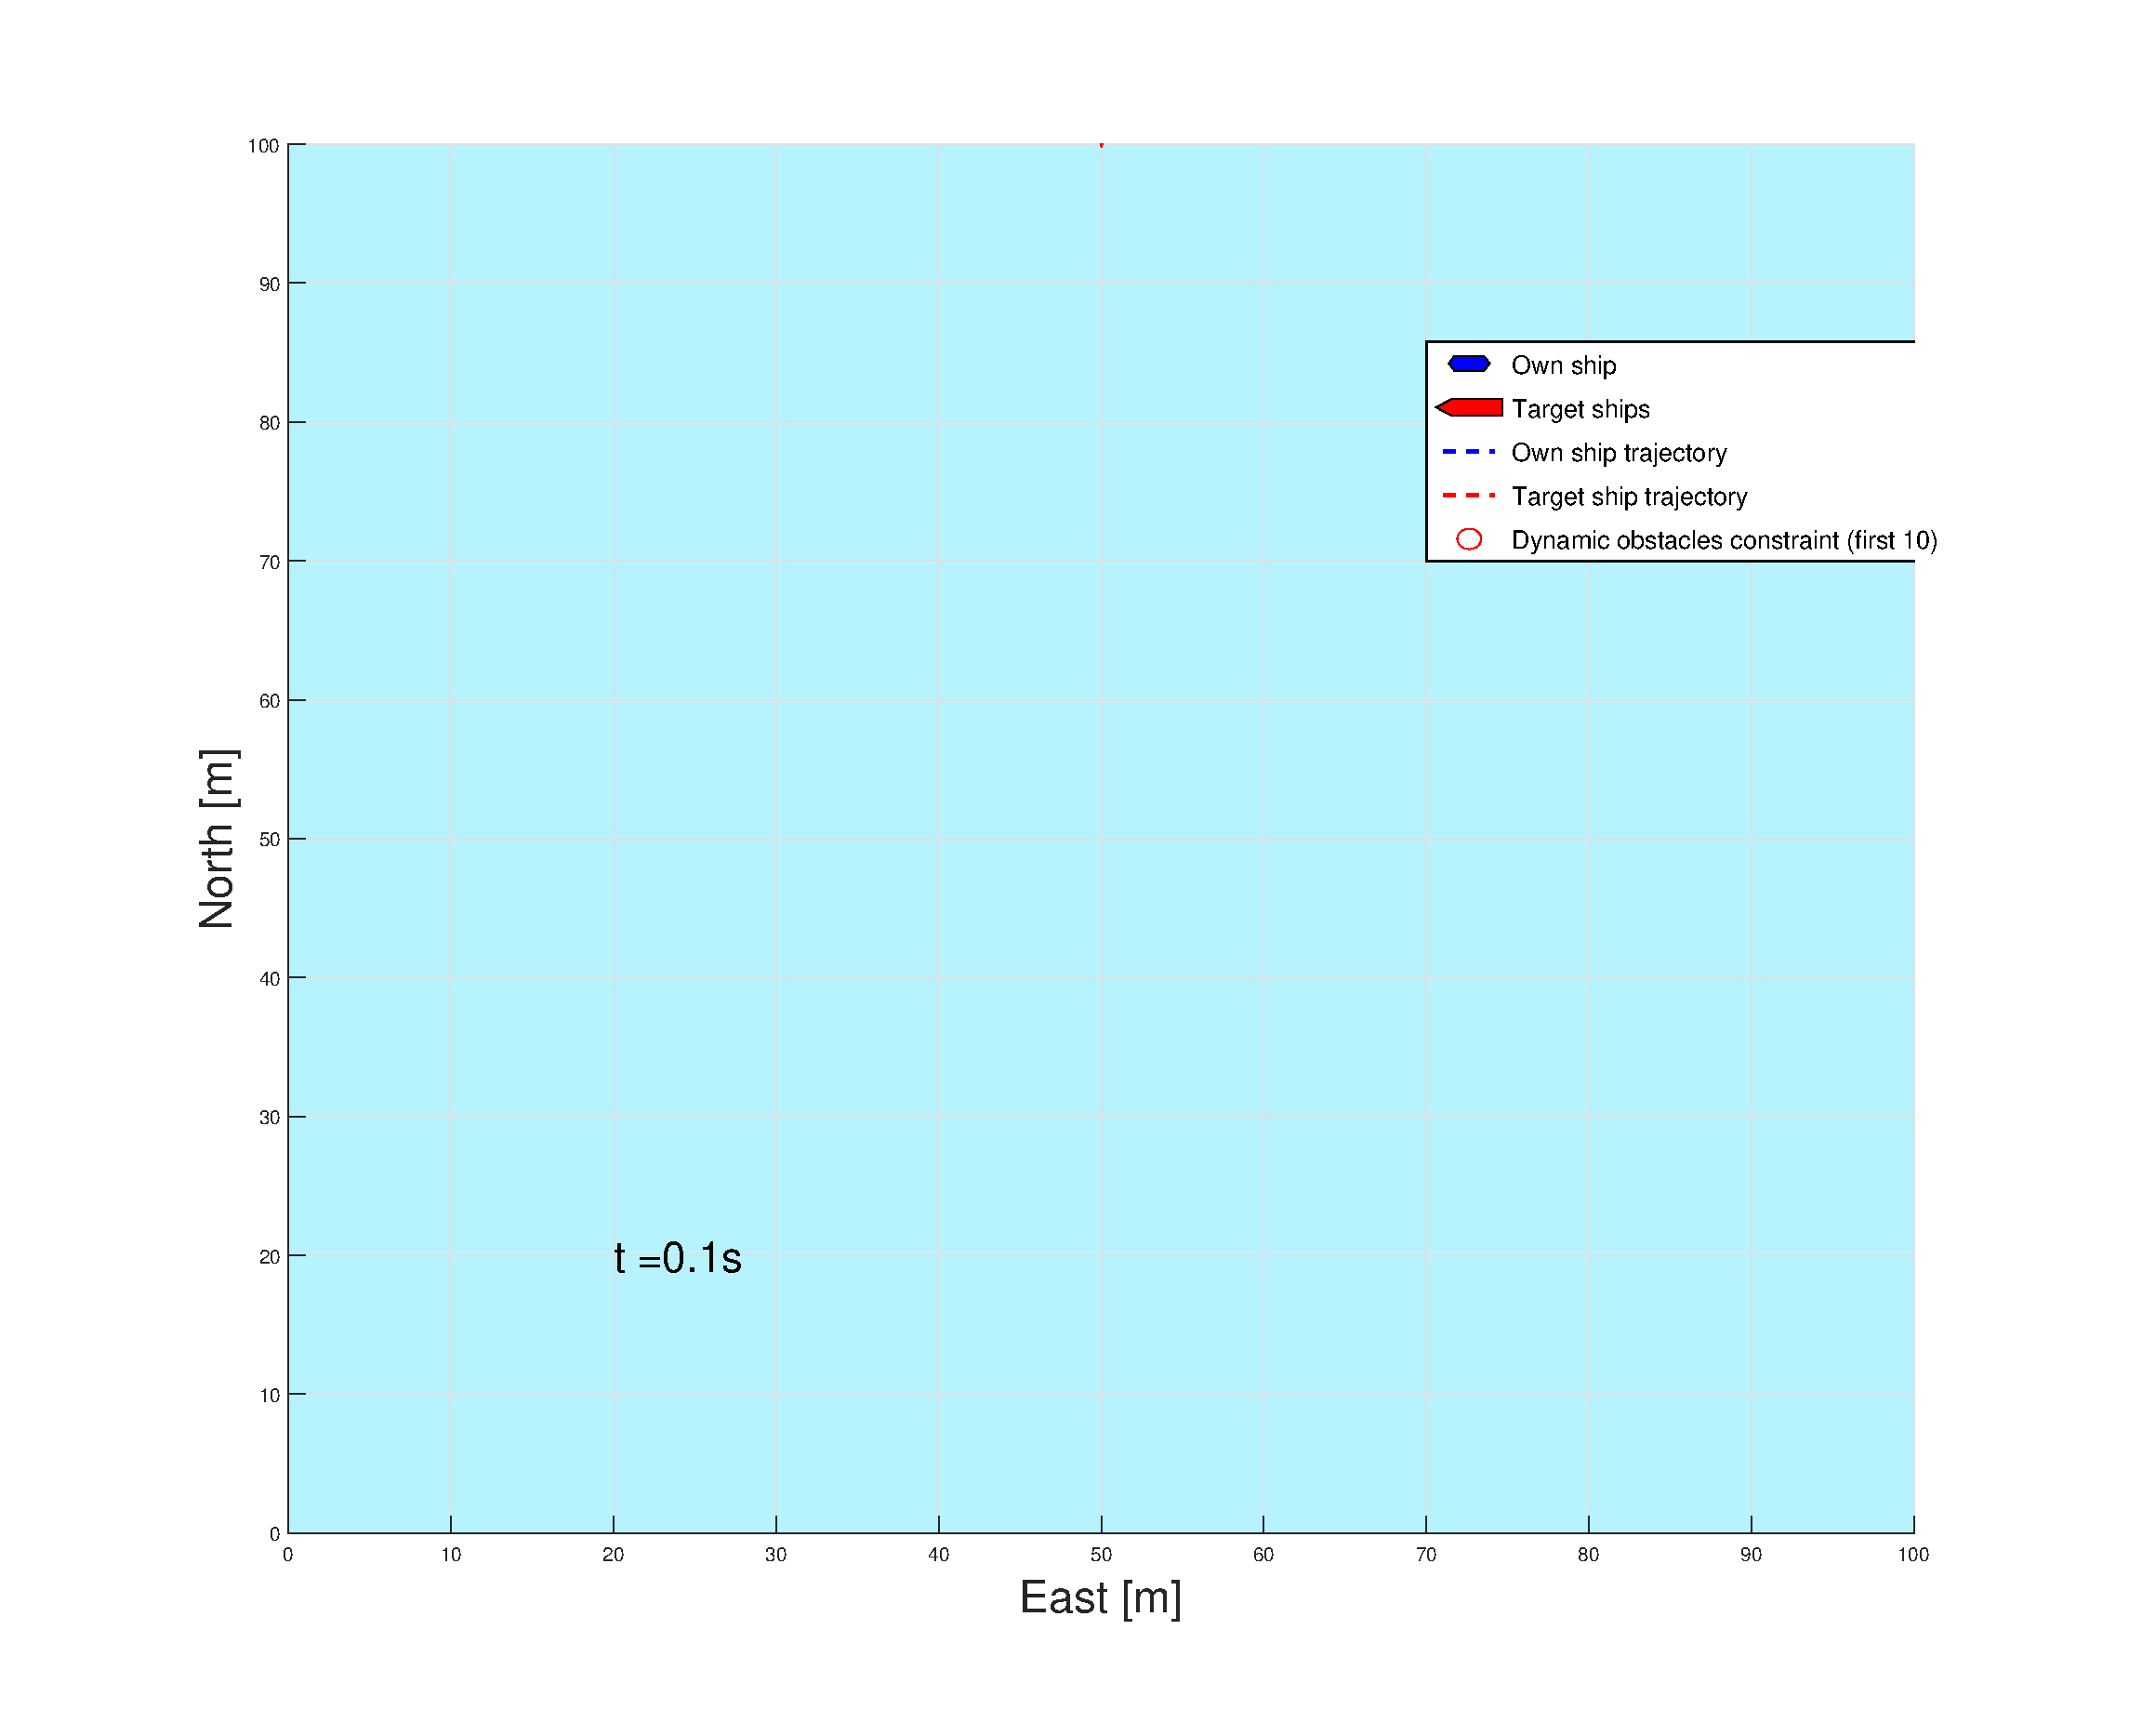
\includegraphics[width=\textwidth]{Images/Figures/enkel_HO/_Simple_0fig1_time=0}
        \subcaption{caption}
    \end{subfigure}
    \hfill
    \begin{subfigure}[b]{0.499\textwidth}
        \centering
        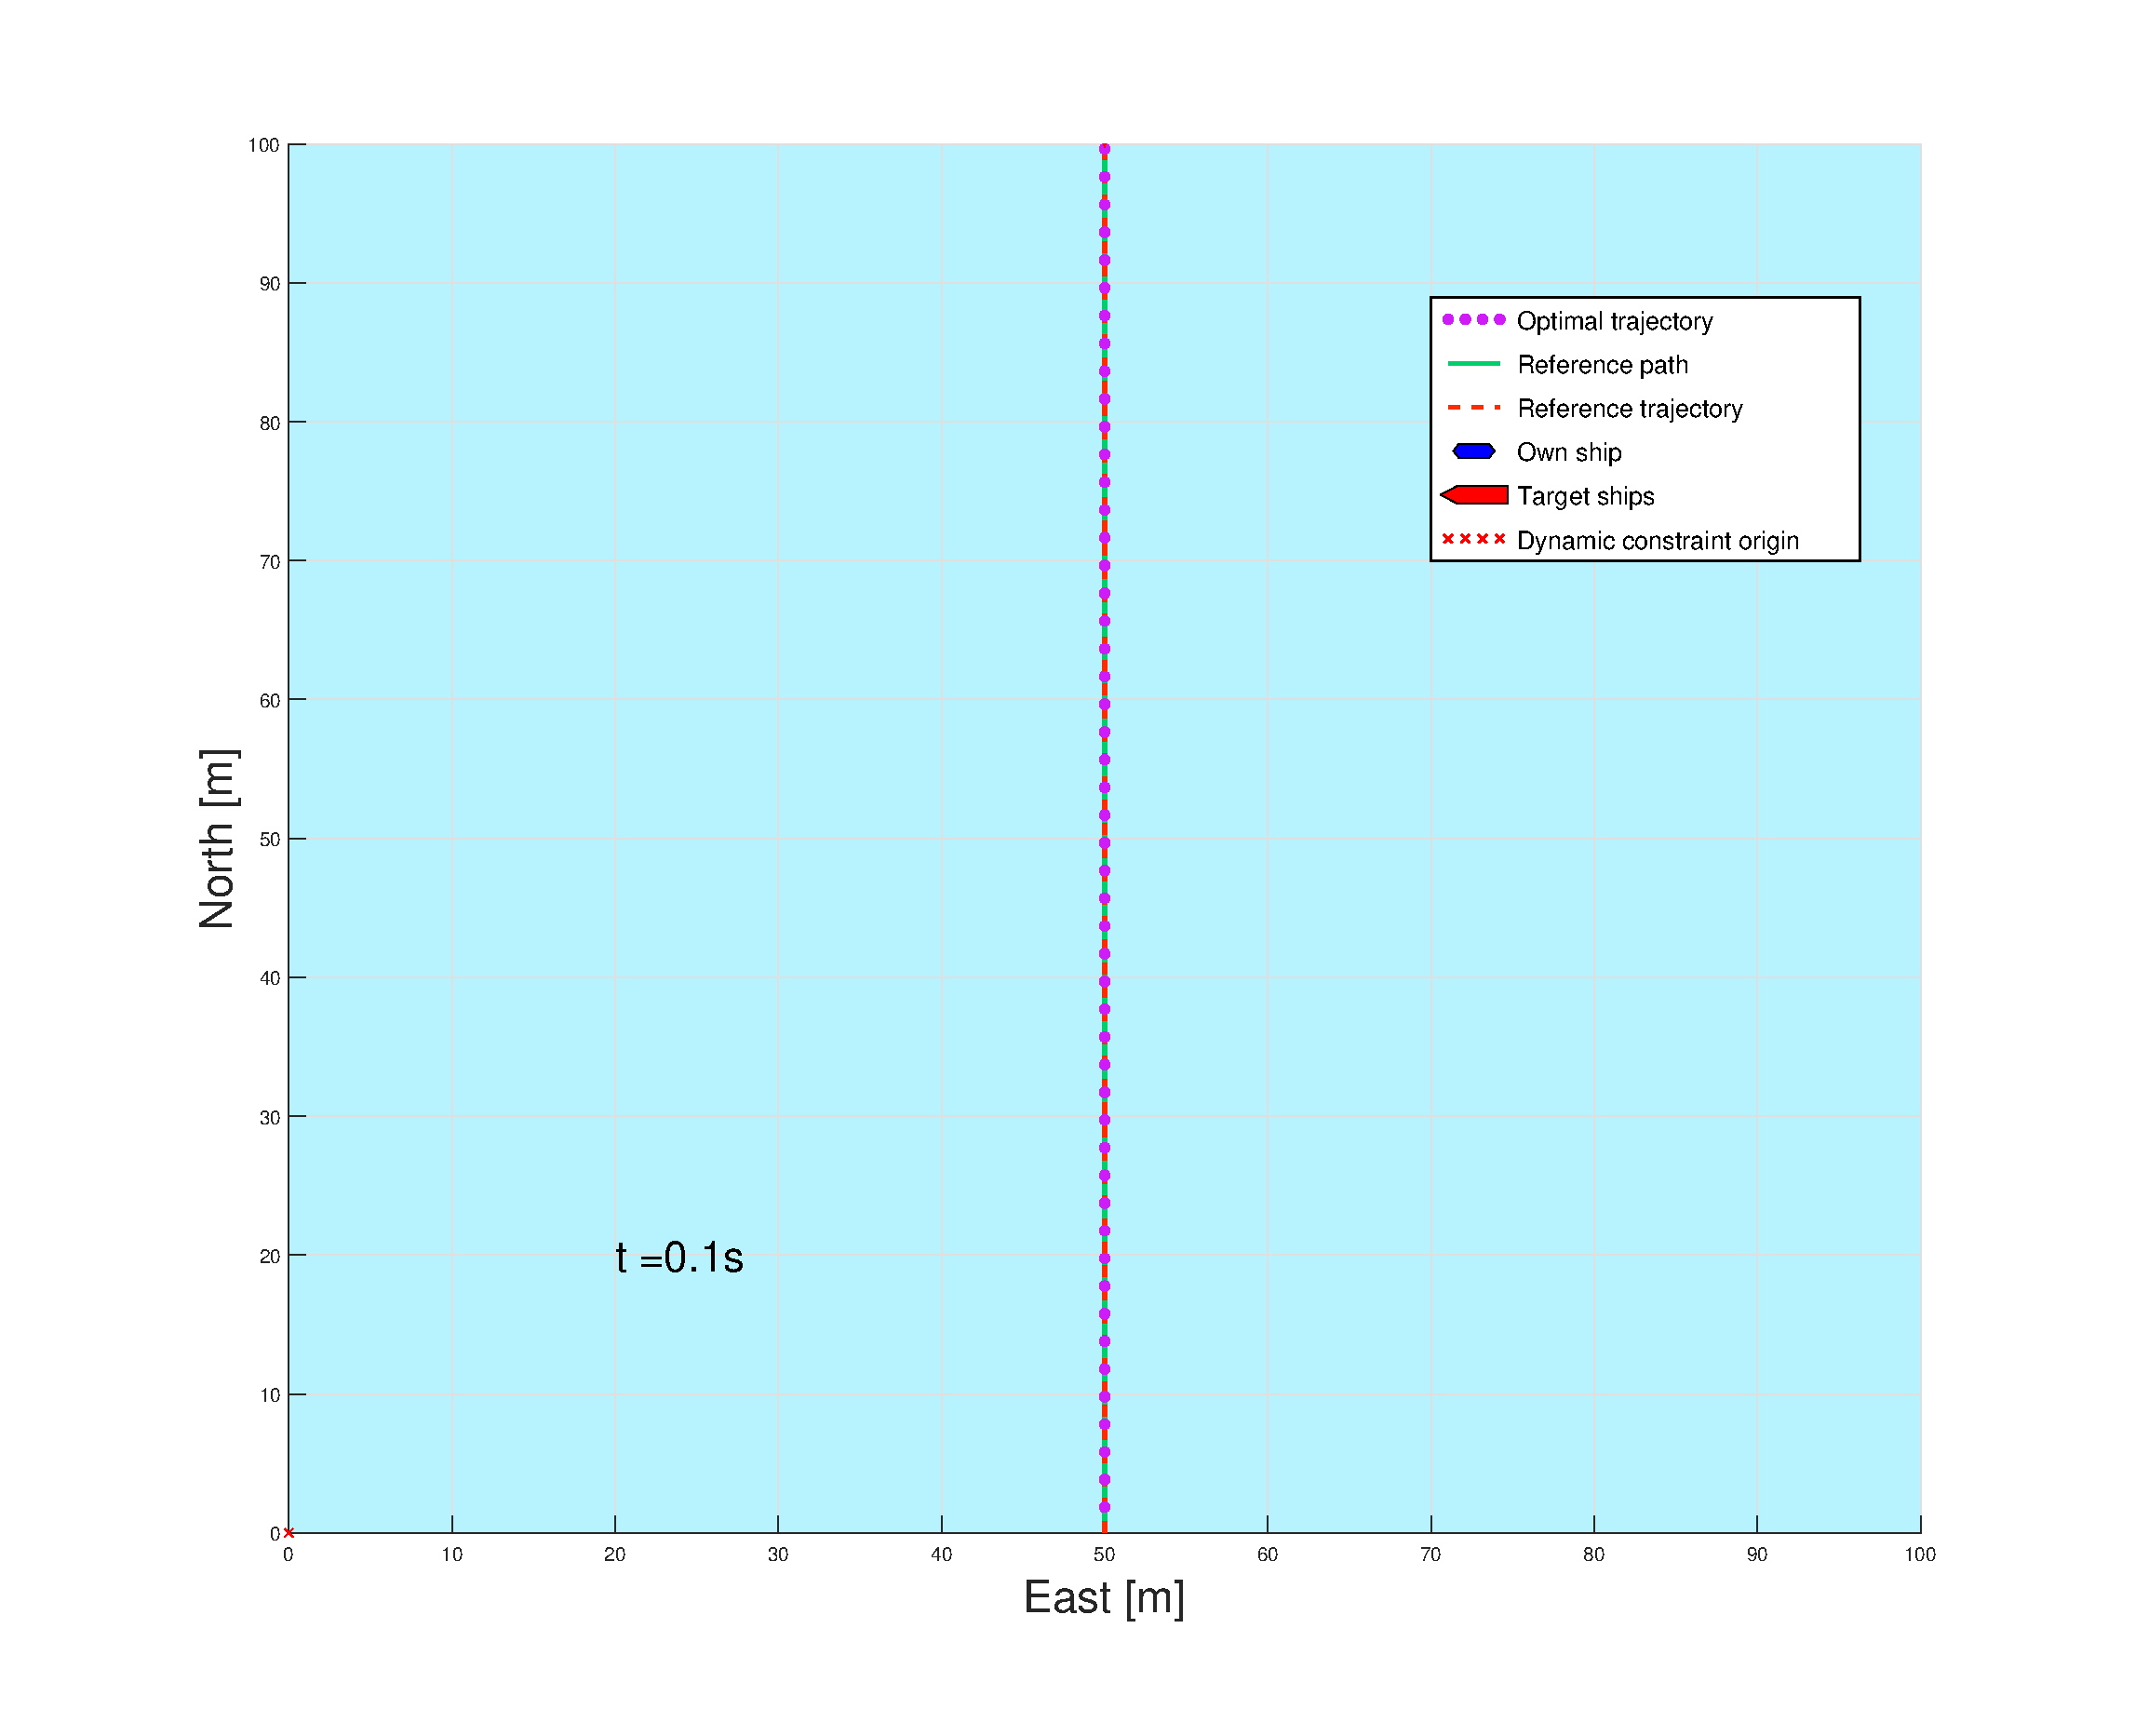
\includegraphics[width=\textwidth]{Images/Figures/enkel_HO/_Simple_0fig999_time=0}
        \subcaption{mhm}
    \end{subfigure}
    \hfill
    \\
    \begin{subfigure}[b]{0.49\textwidth}
        \centering
        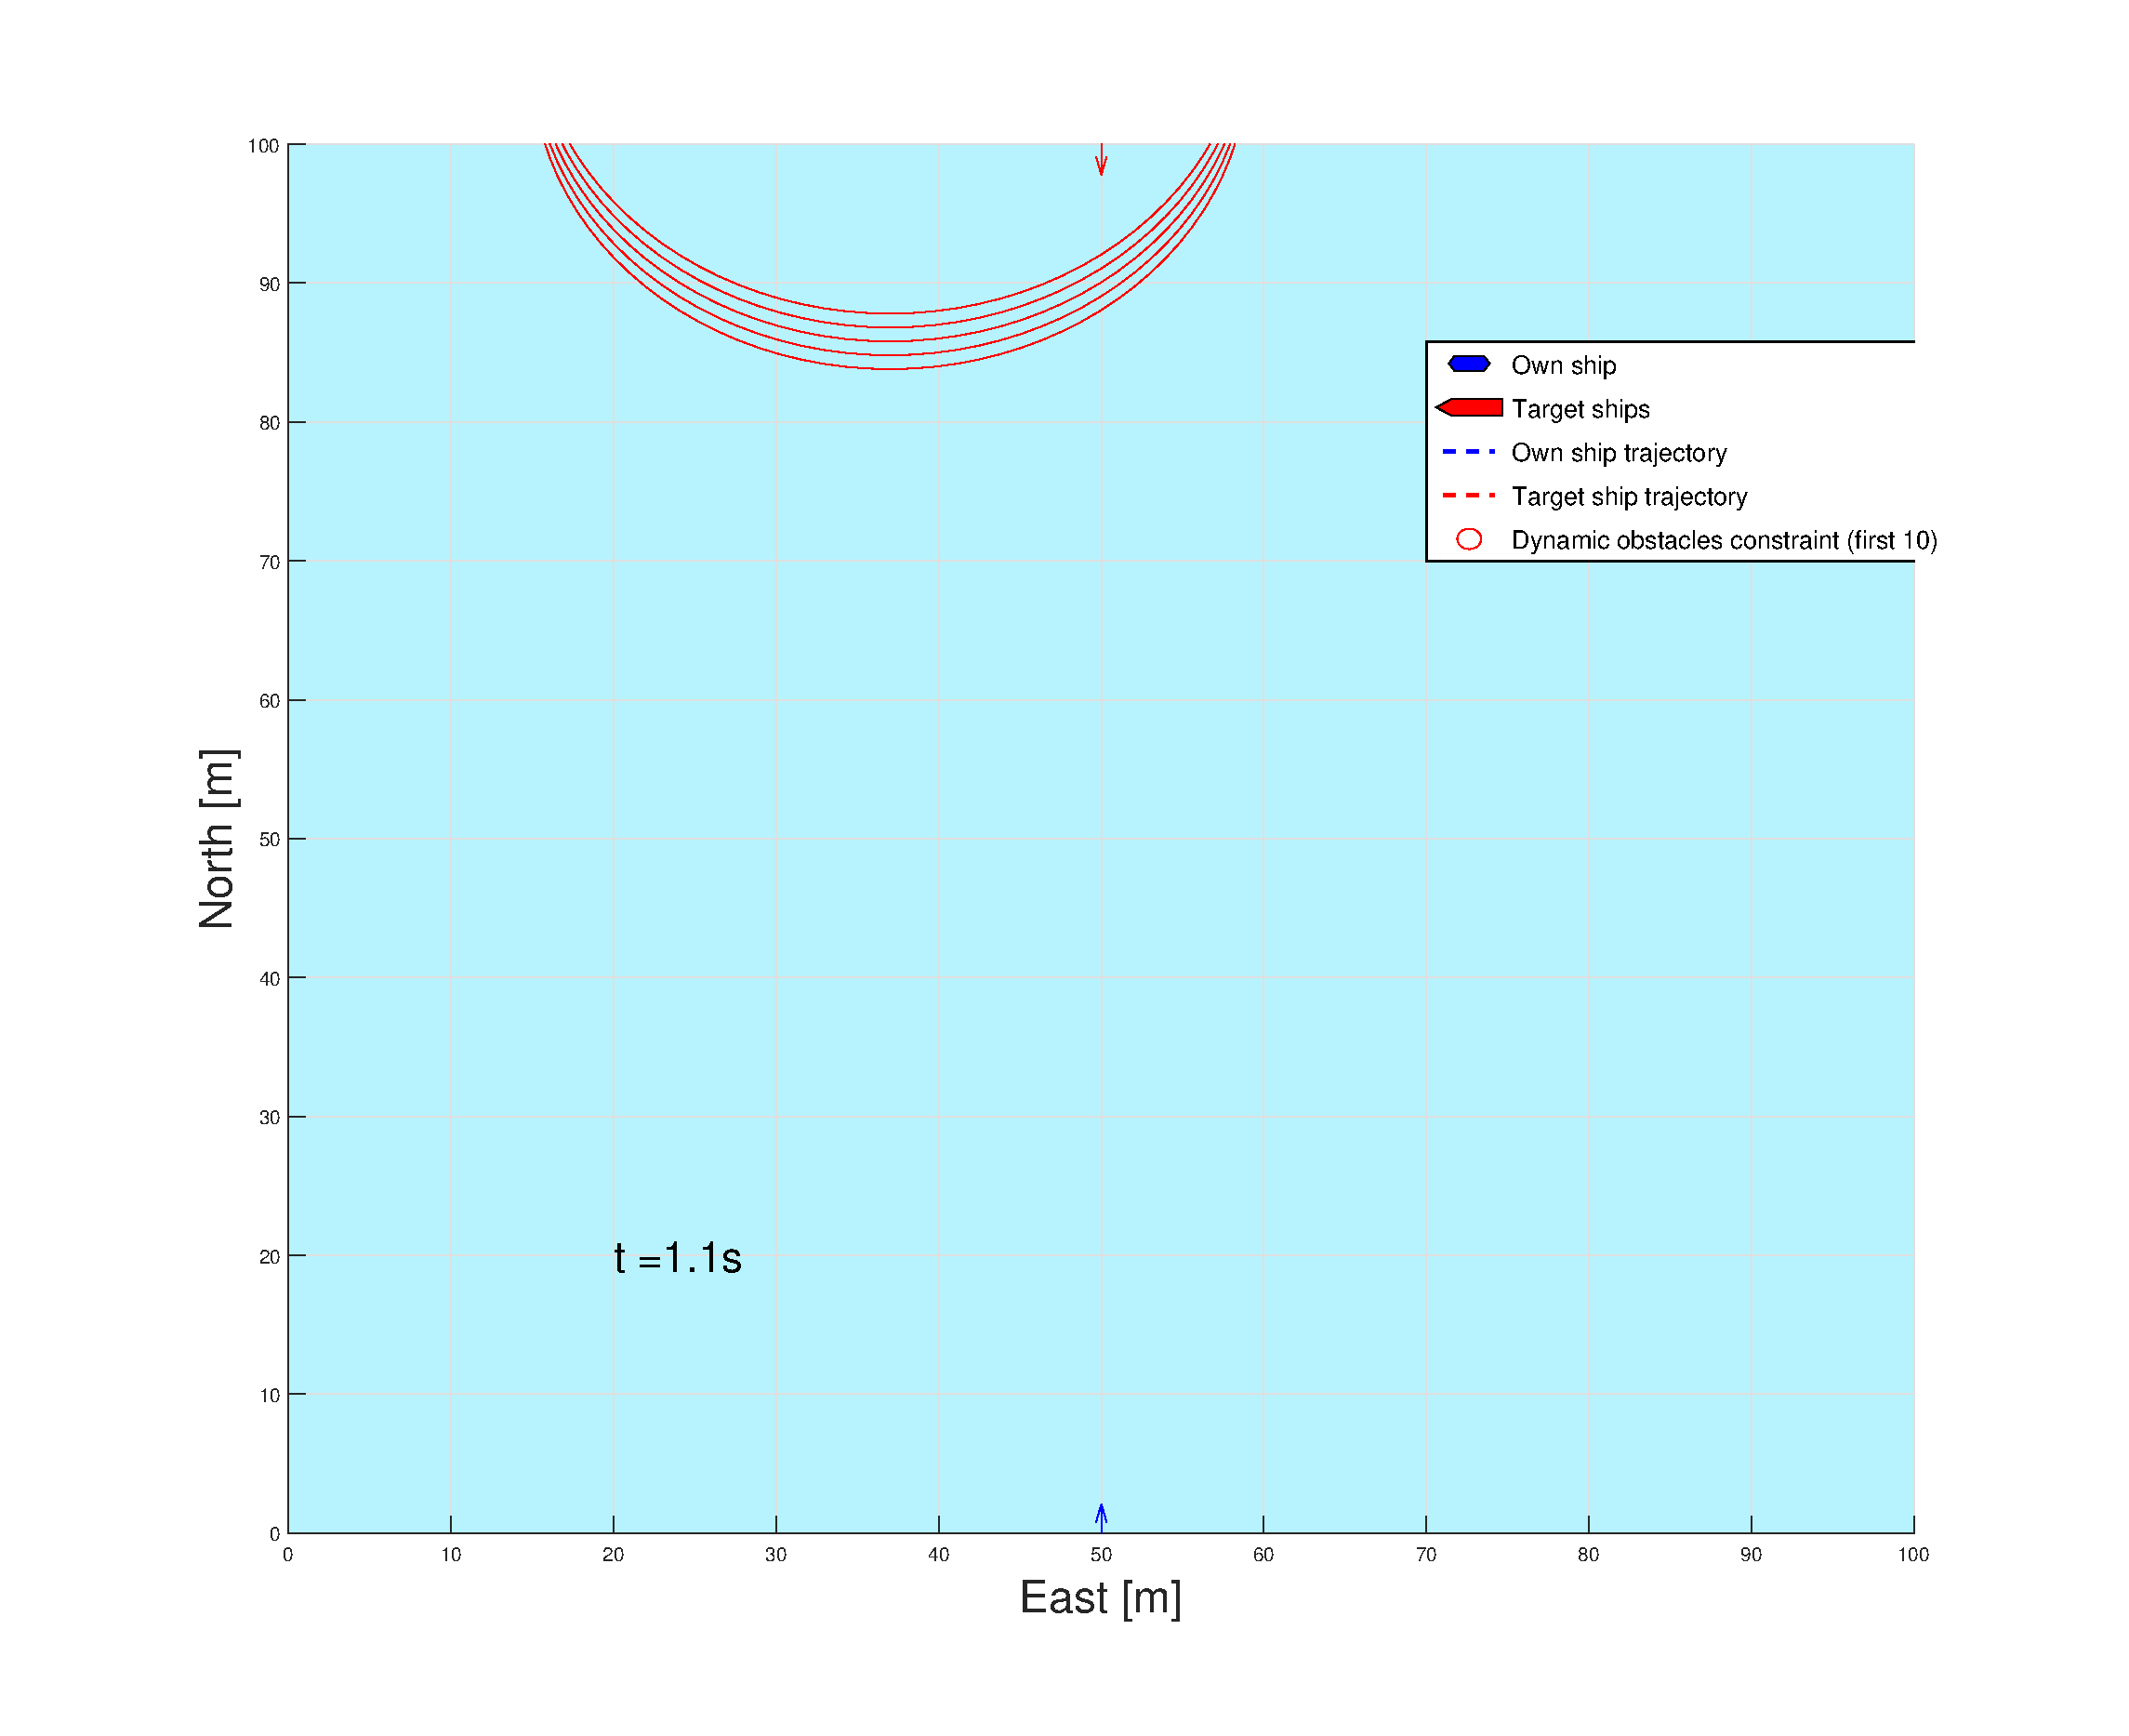
\includegraphics[width=\textwidth]{Images/Figures/enkel_HO/_Simple_0fig1_time=1}
        \subcaption{caption}
    \end{subfigure}
    \hfill
    \begin{subfigure}[b]{0.499\textwidth}
        \centering
        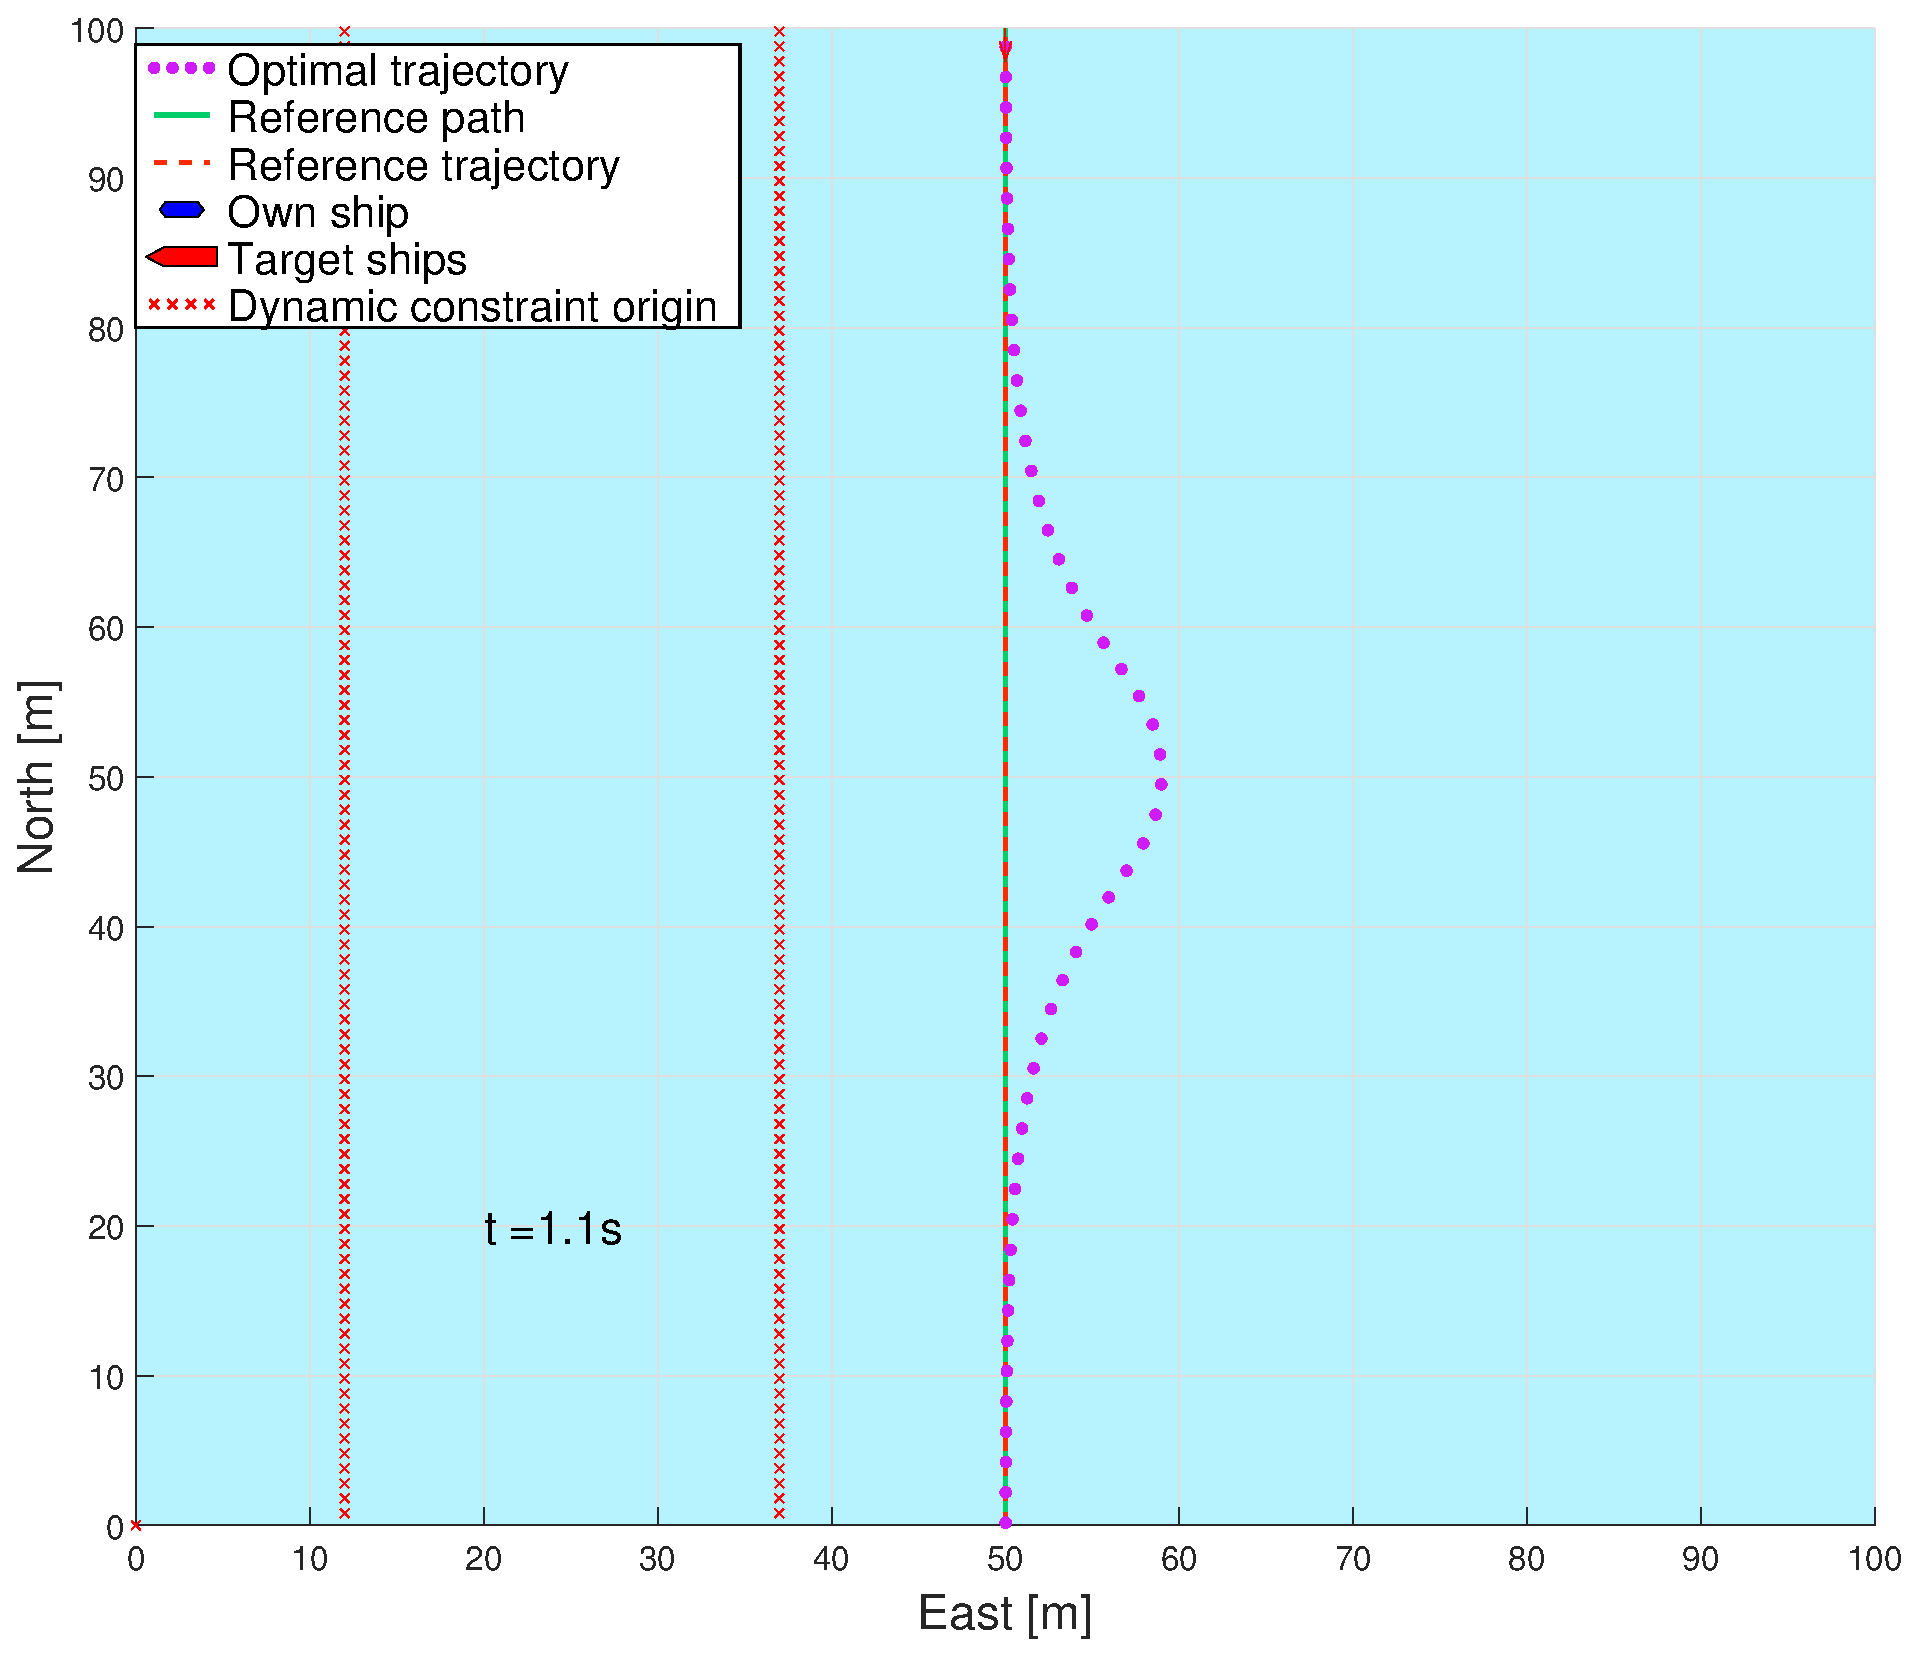
\includegraphics[width=\textwidth]{Images/Figures/enkel_HO/_Simple_0fig999_time=1}
        \subcaption{mhm}
    \end{subfigure}
    \hfill
    \\
    \begin{subfigure}[b]{0.49\textwidth}
        \centering
        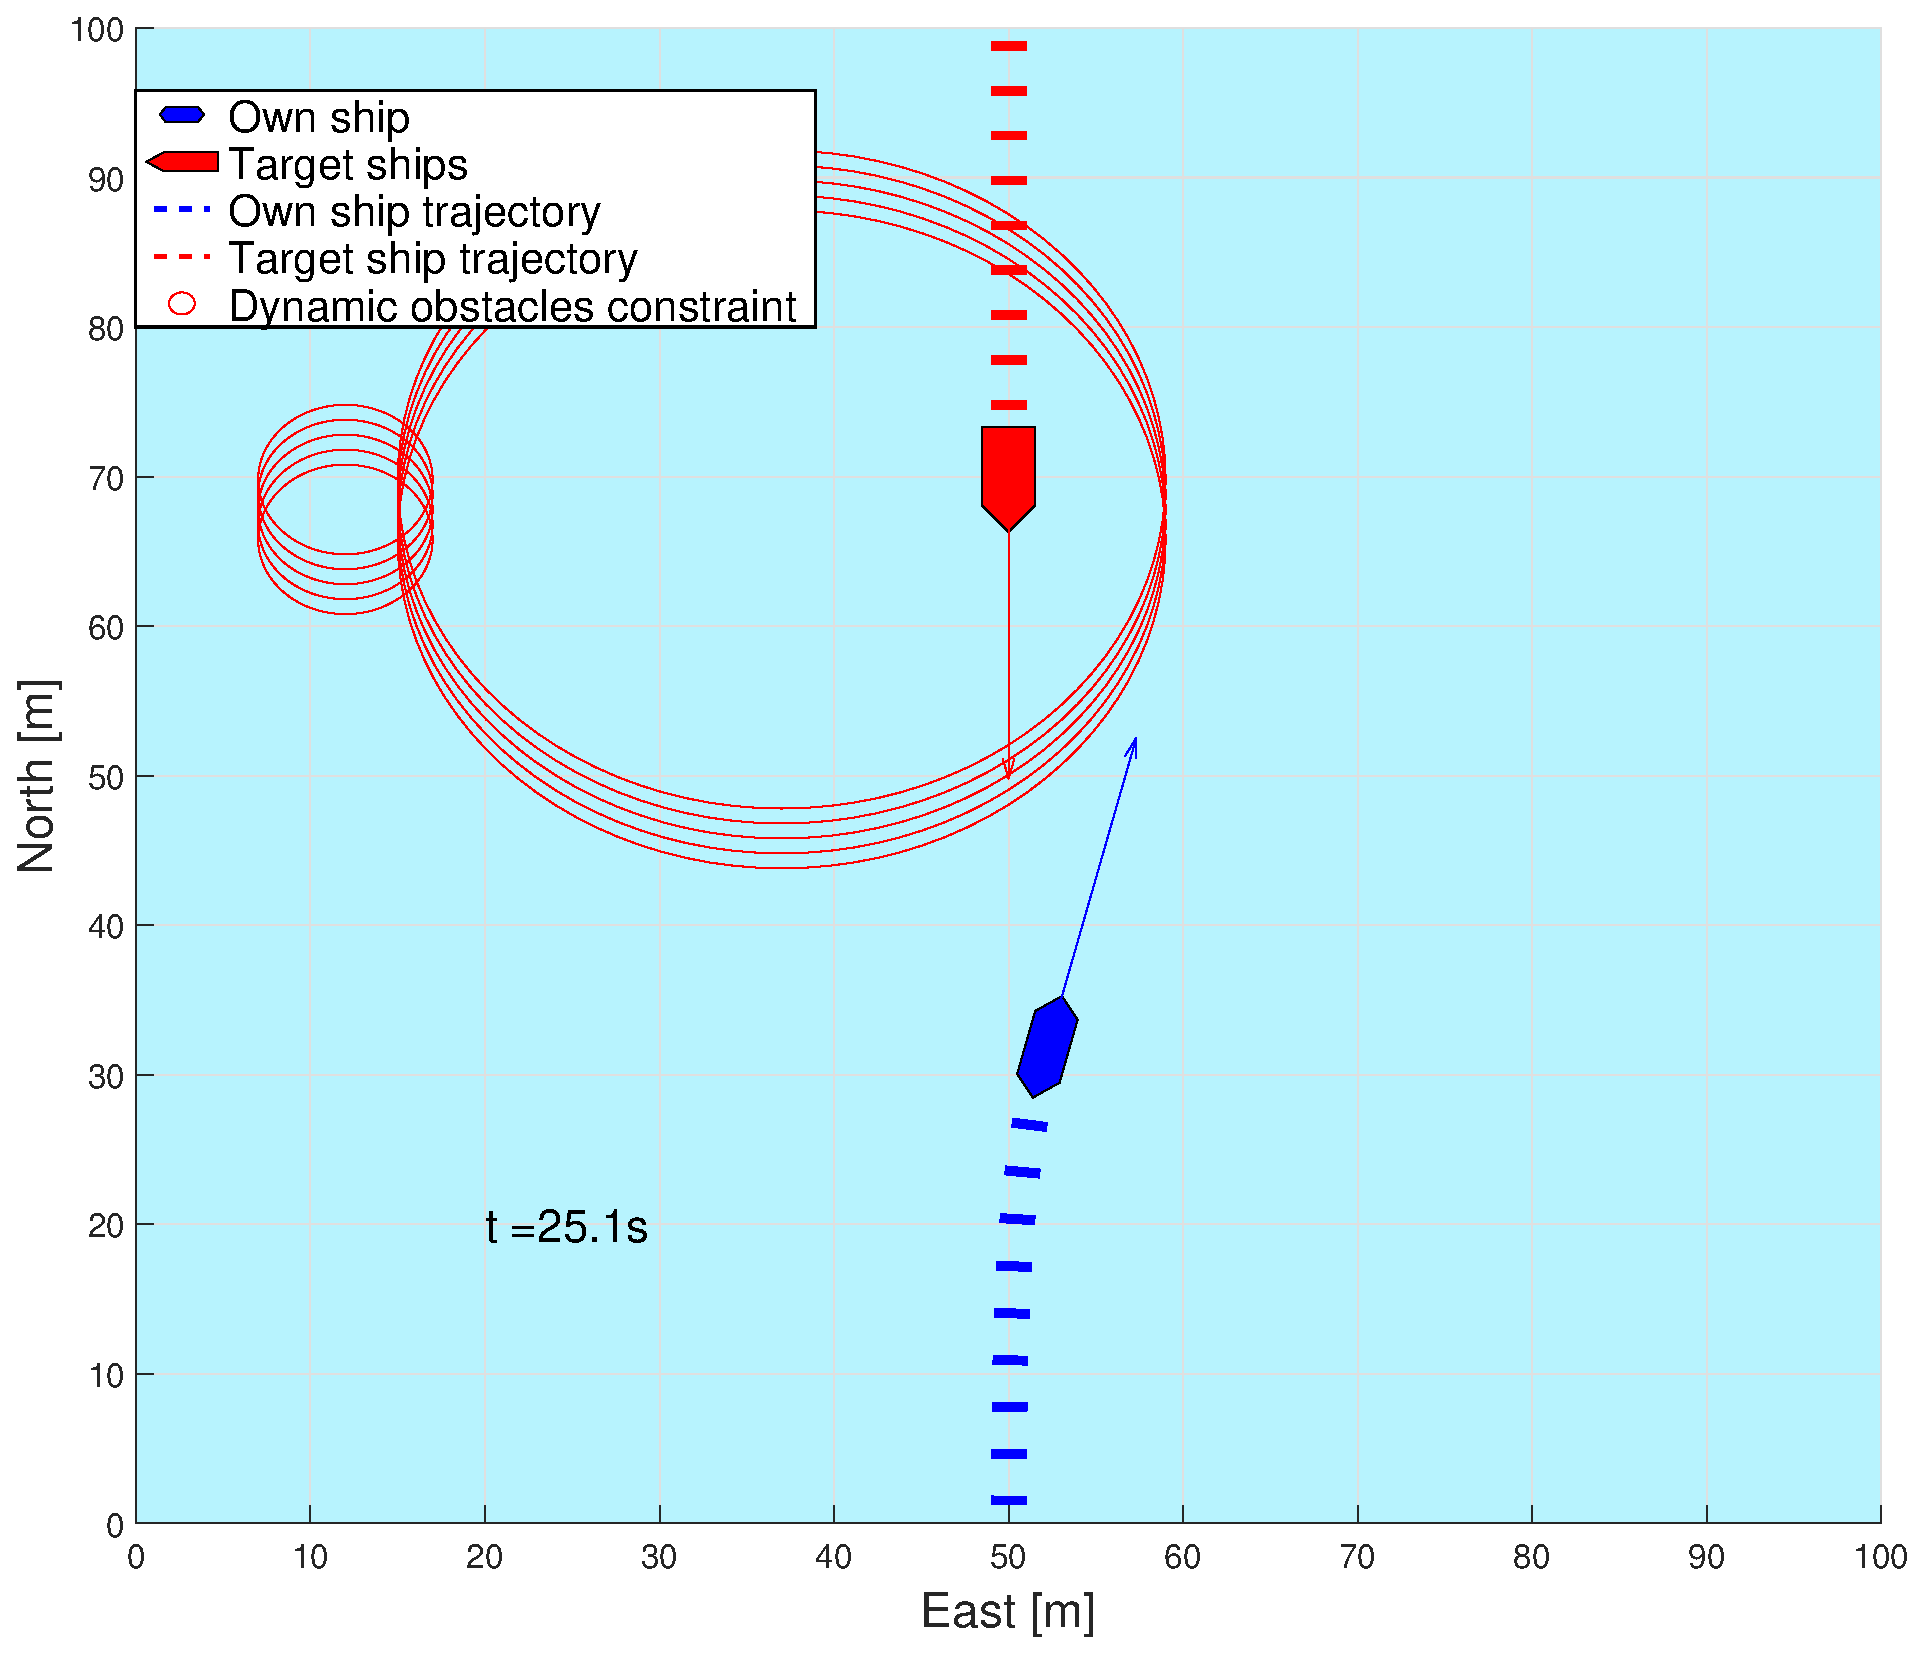
\includegraphics[width=\textwidth]{Images/Figures/enkel_HO/_Simple_0fig1_time=25}
        \subcaption{caption}
    \end{subfigure}
    \hfill
    \begin{subfigure}[b]{0.499\textwidth}
        \centering
        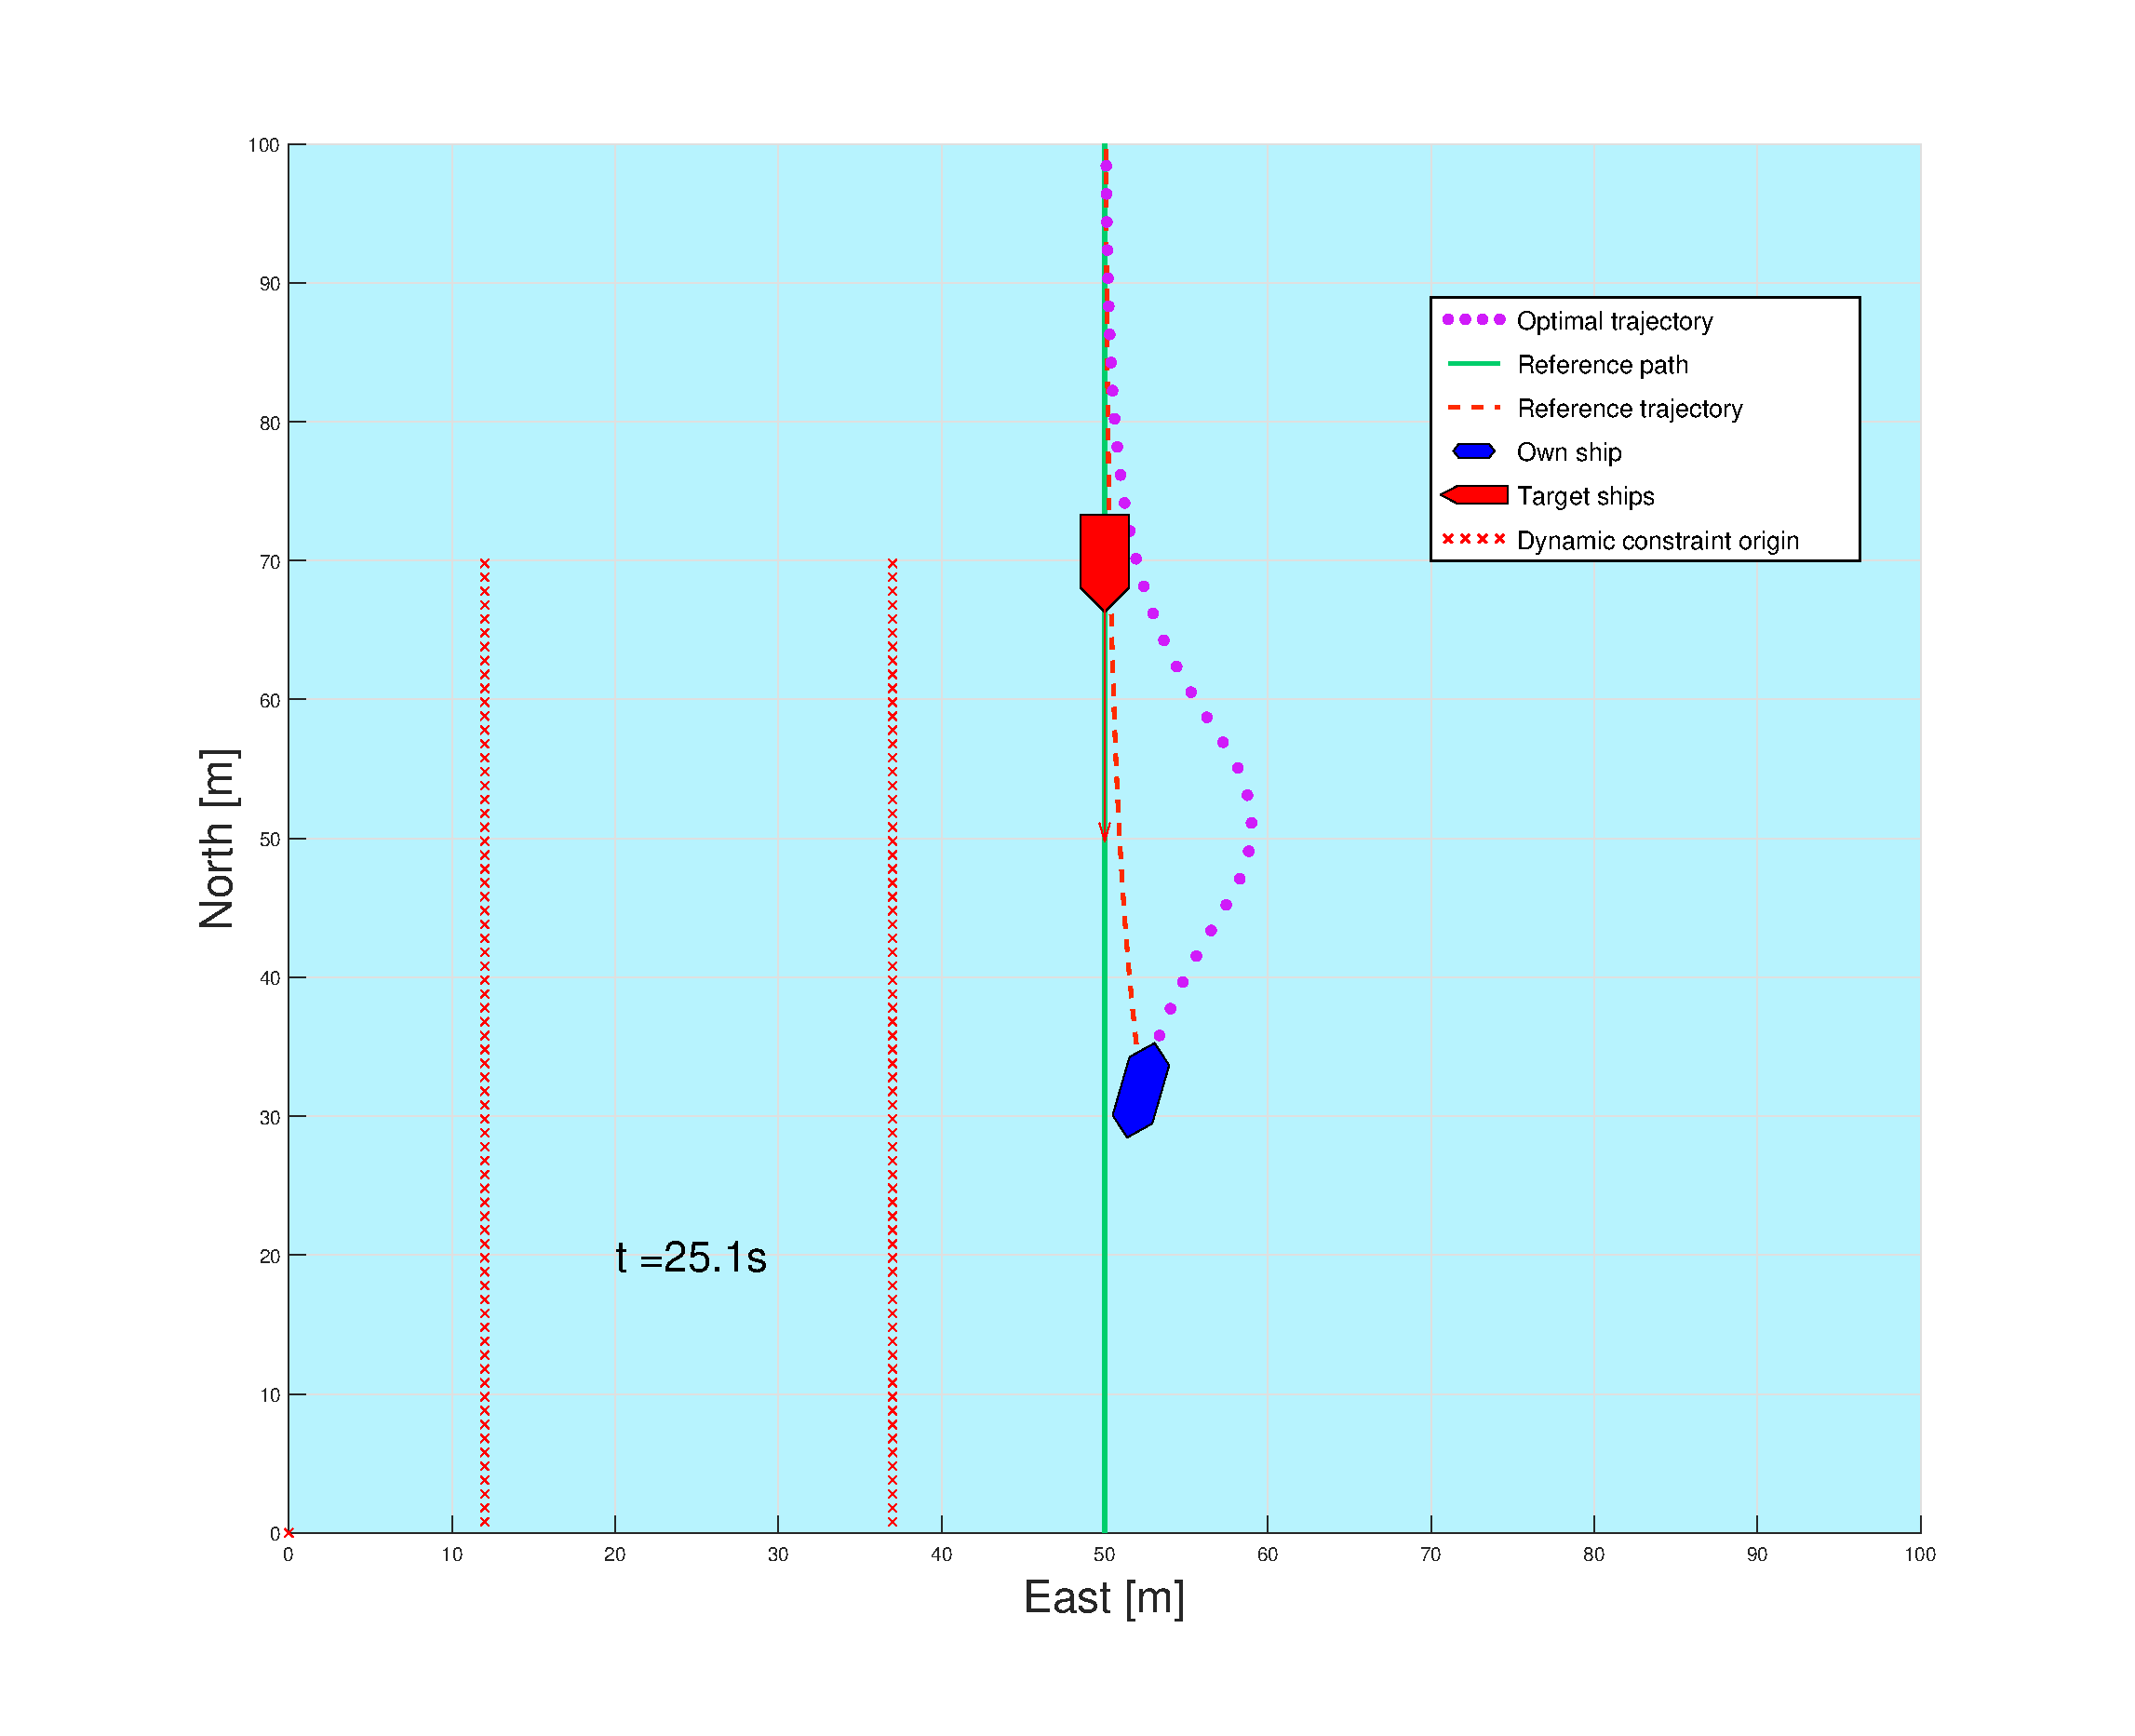
\includegraphics[width=\textwidth]{Images/Figures/enkel_HO/_Simple_0fig999_time=25}
        \subcaption{mhm}
    \end{subfigure}
    \hfill
\end{figure}%
\begin{figure}[ht]\ContinuedFloat
    \begin{subfigure}[b]{0.49\textwidth}
        \centering
        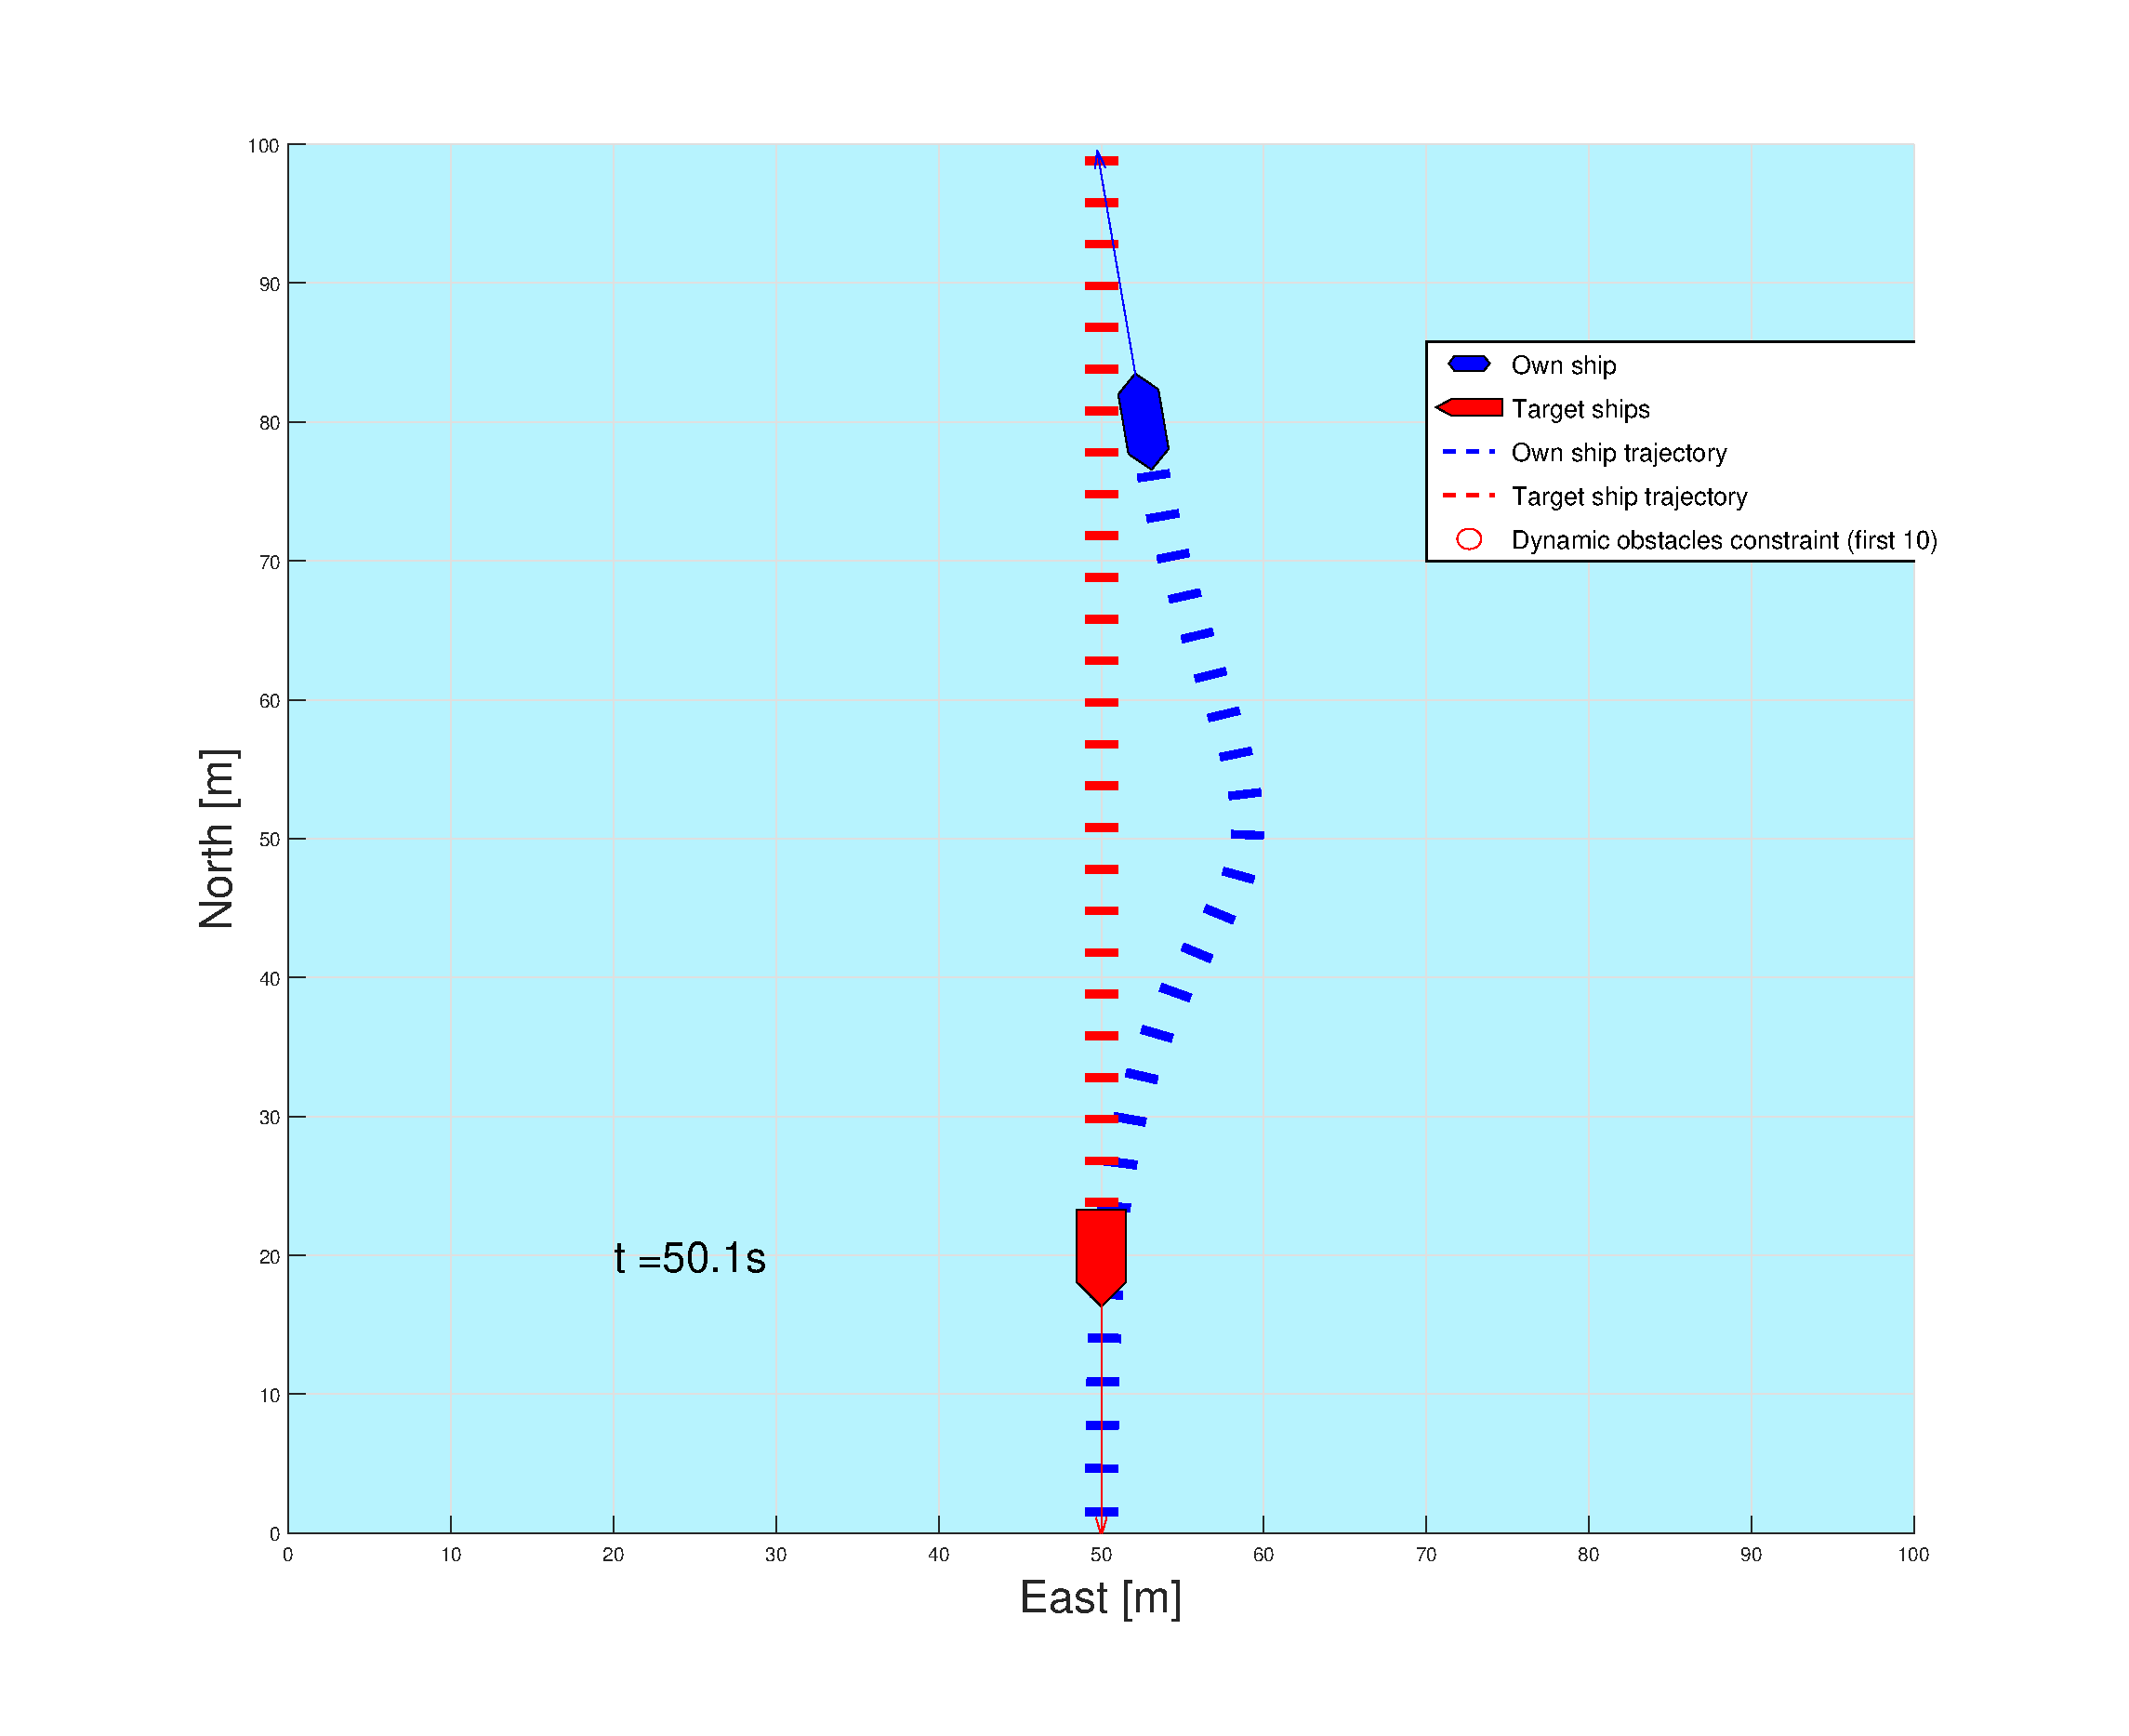
\includegraphics[width=\textwidth]{Images/Figures/enkel_HO/_Simple_0fig1_time=50}
        \subcaption{caption}
    \end{subfigure}
    \hfill
    \begin{subfigure}[b]{0.499\textwidth}
        \centering
        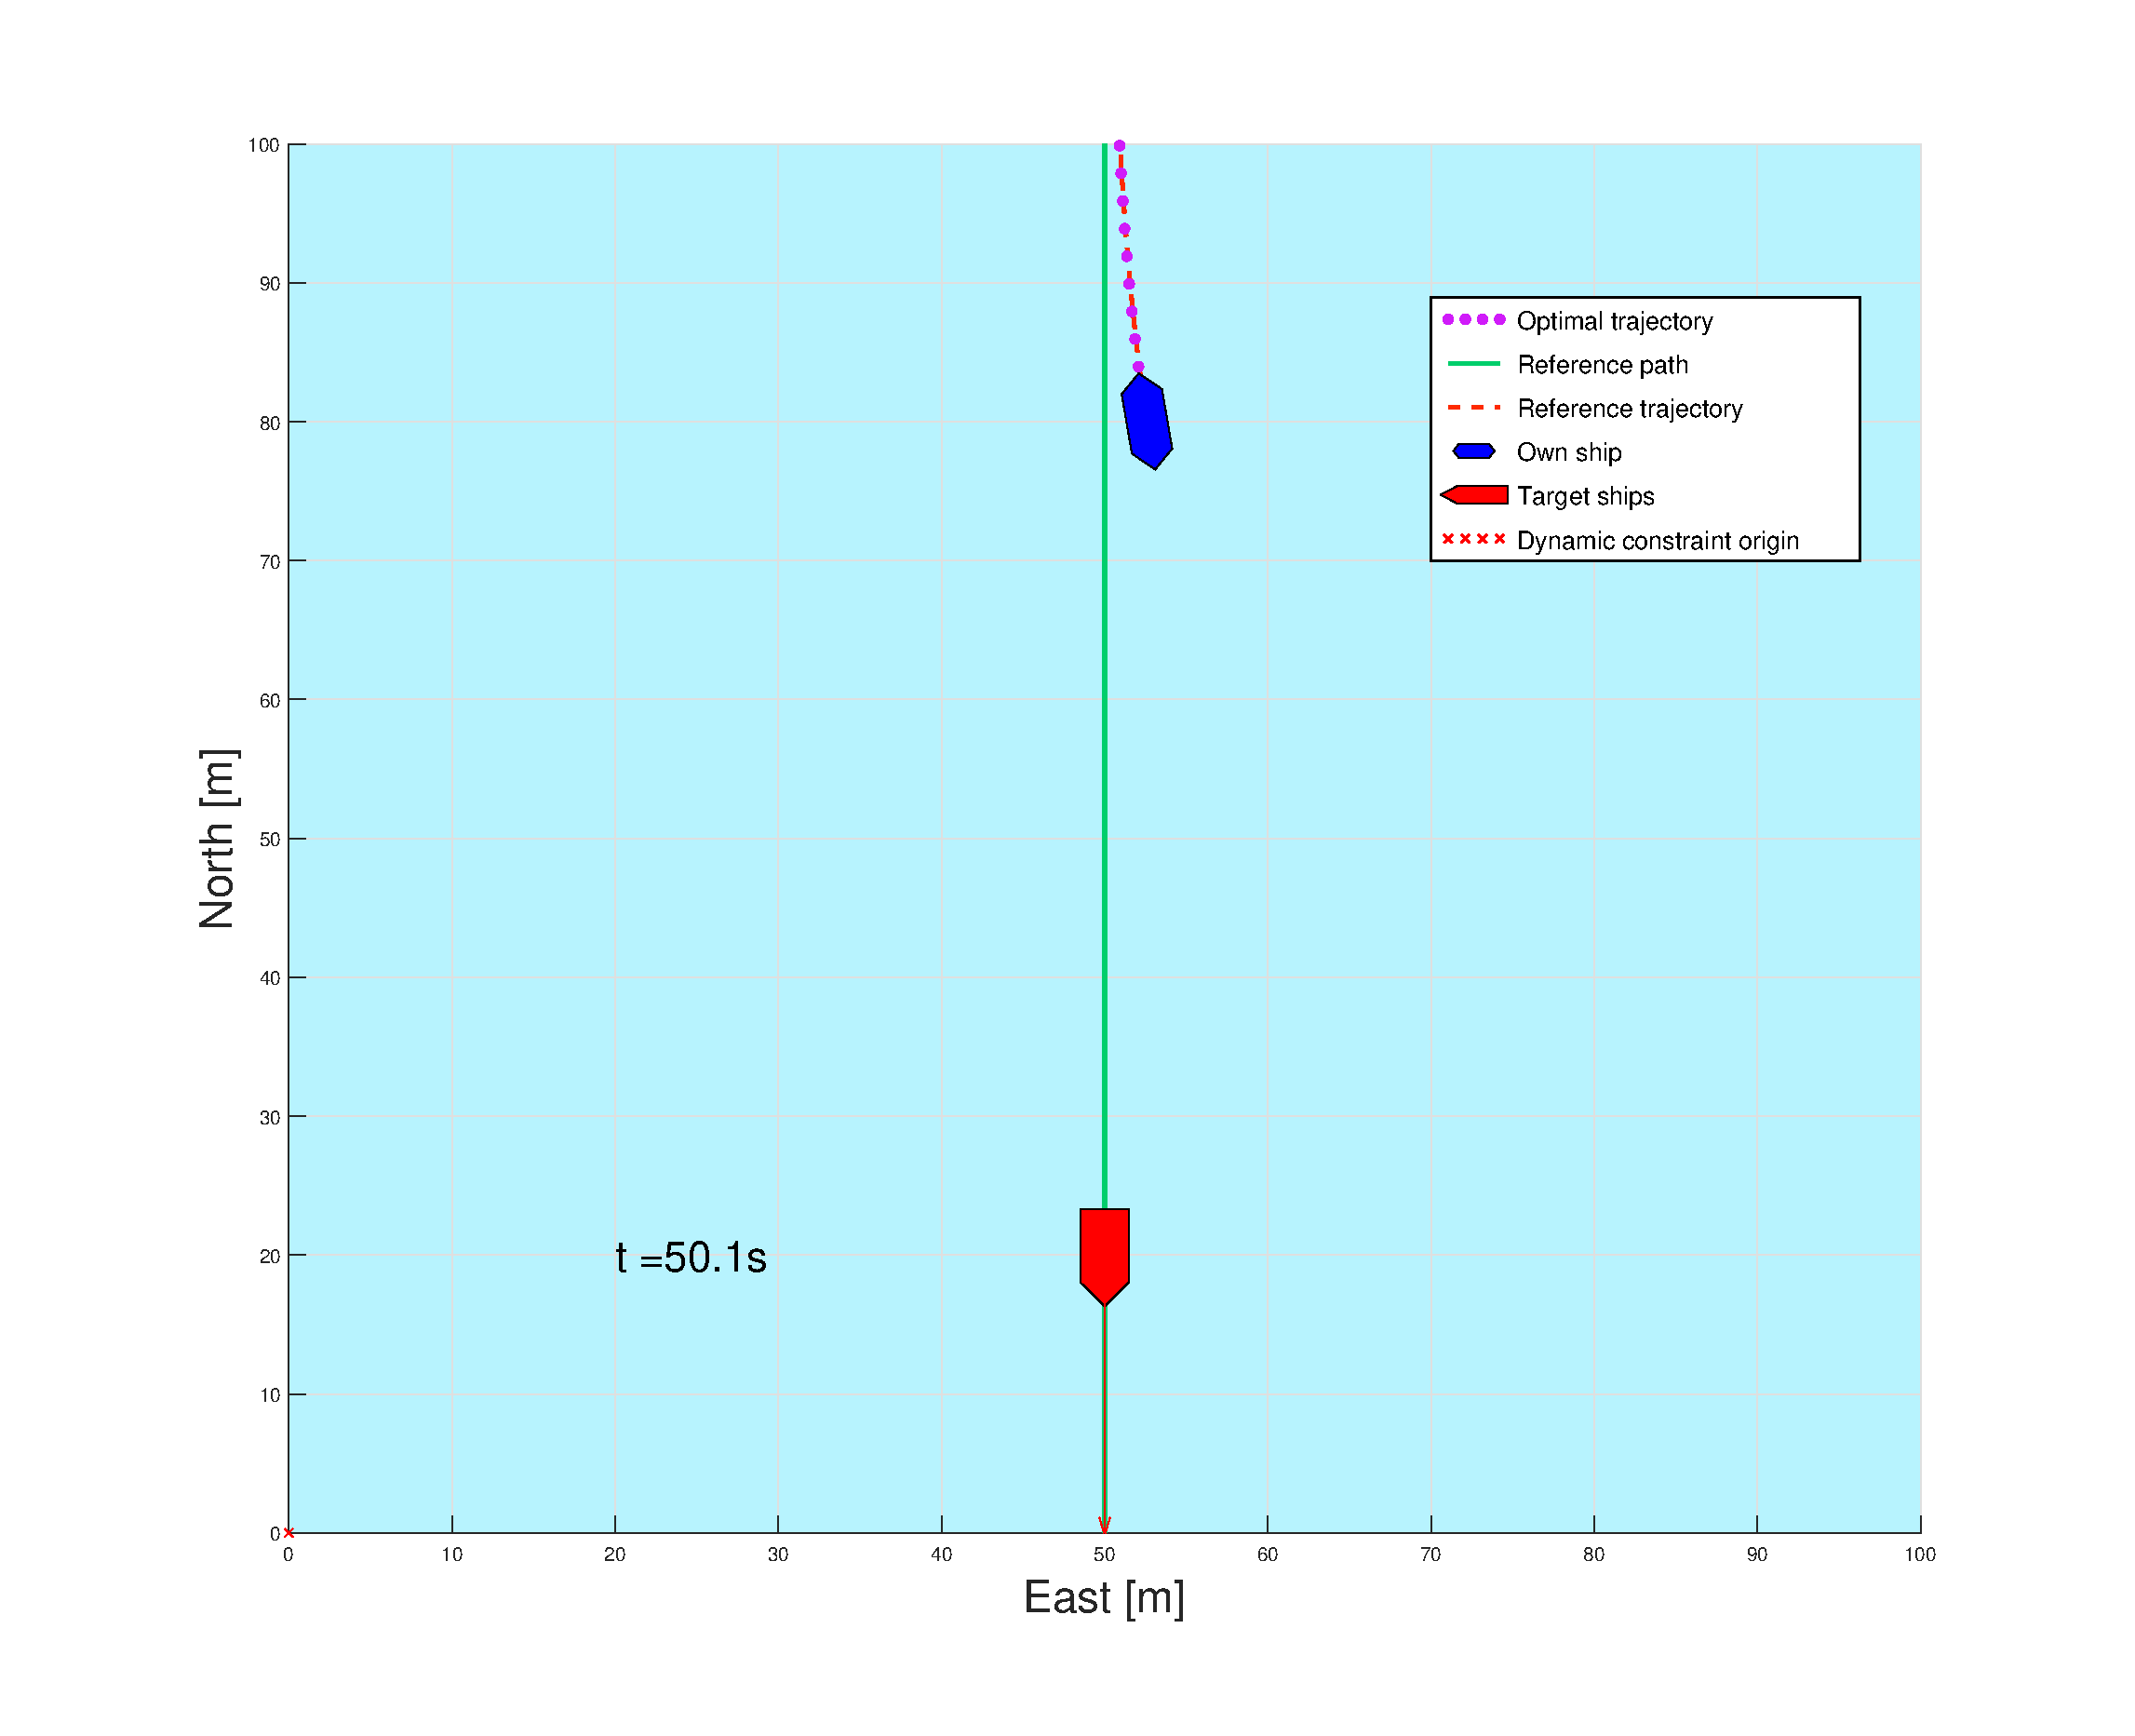
\includegraphics[width=\textwidth]{Images/Figures/enkel_HO/_Simple_0fig999_time=50}
        \subcaption{mhm}
    \end{subfigure}
    \hfill
    \\
    \begin{subfigure}[b]{0.49\textwidth}
        \centering
        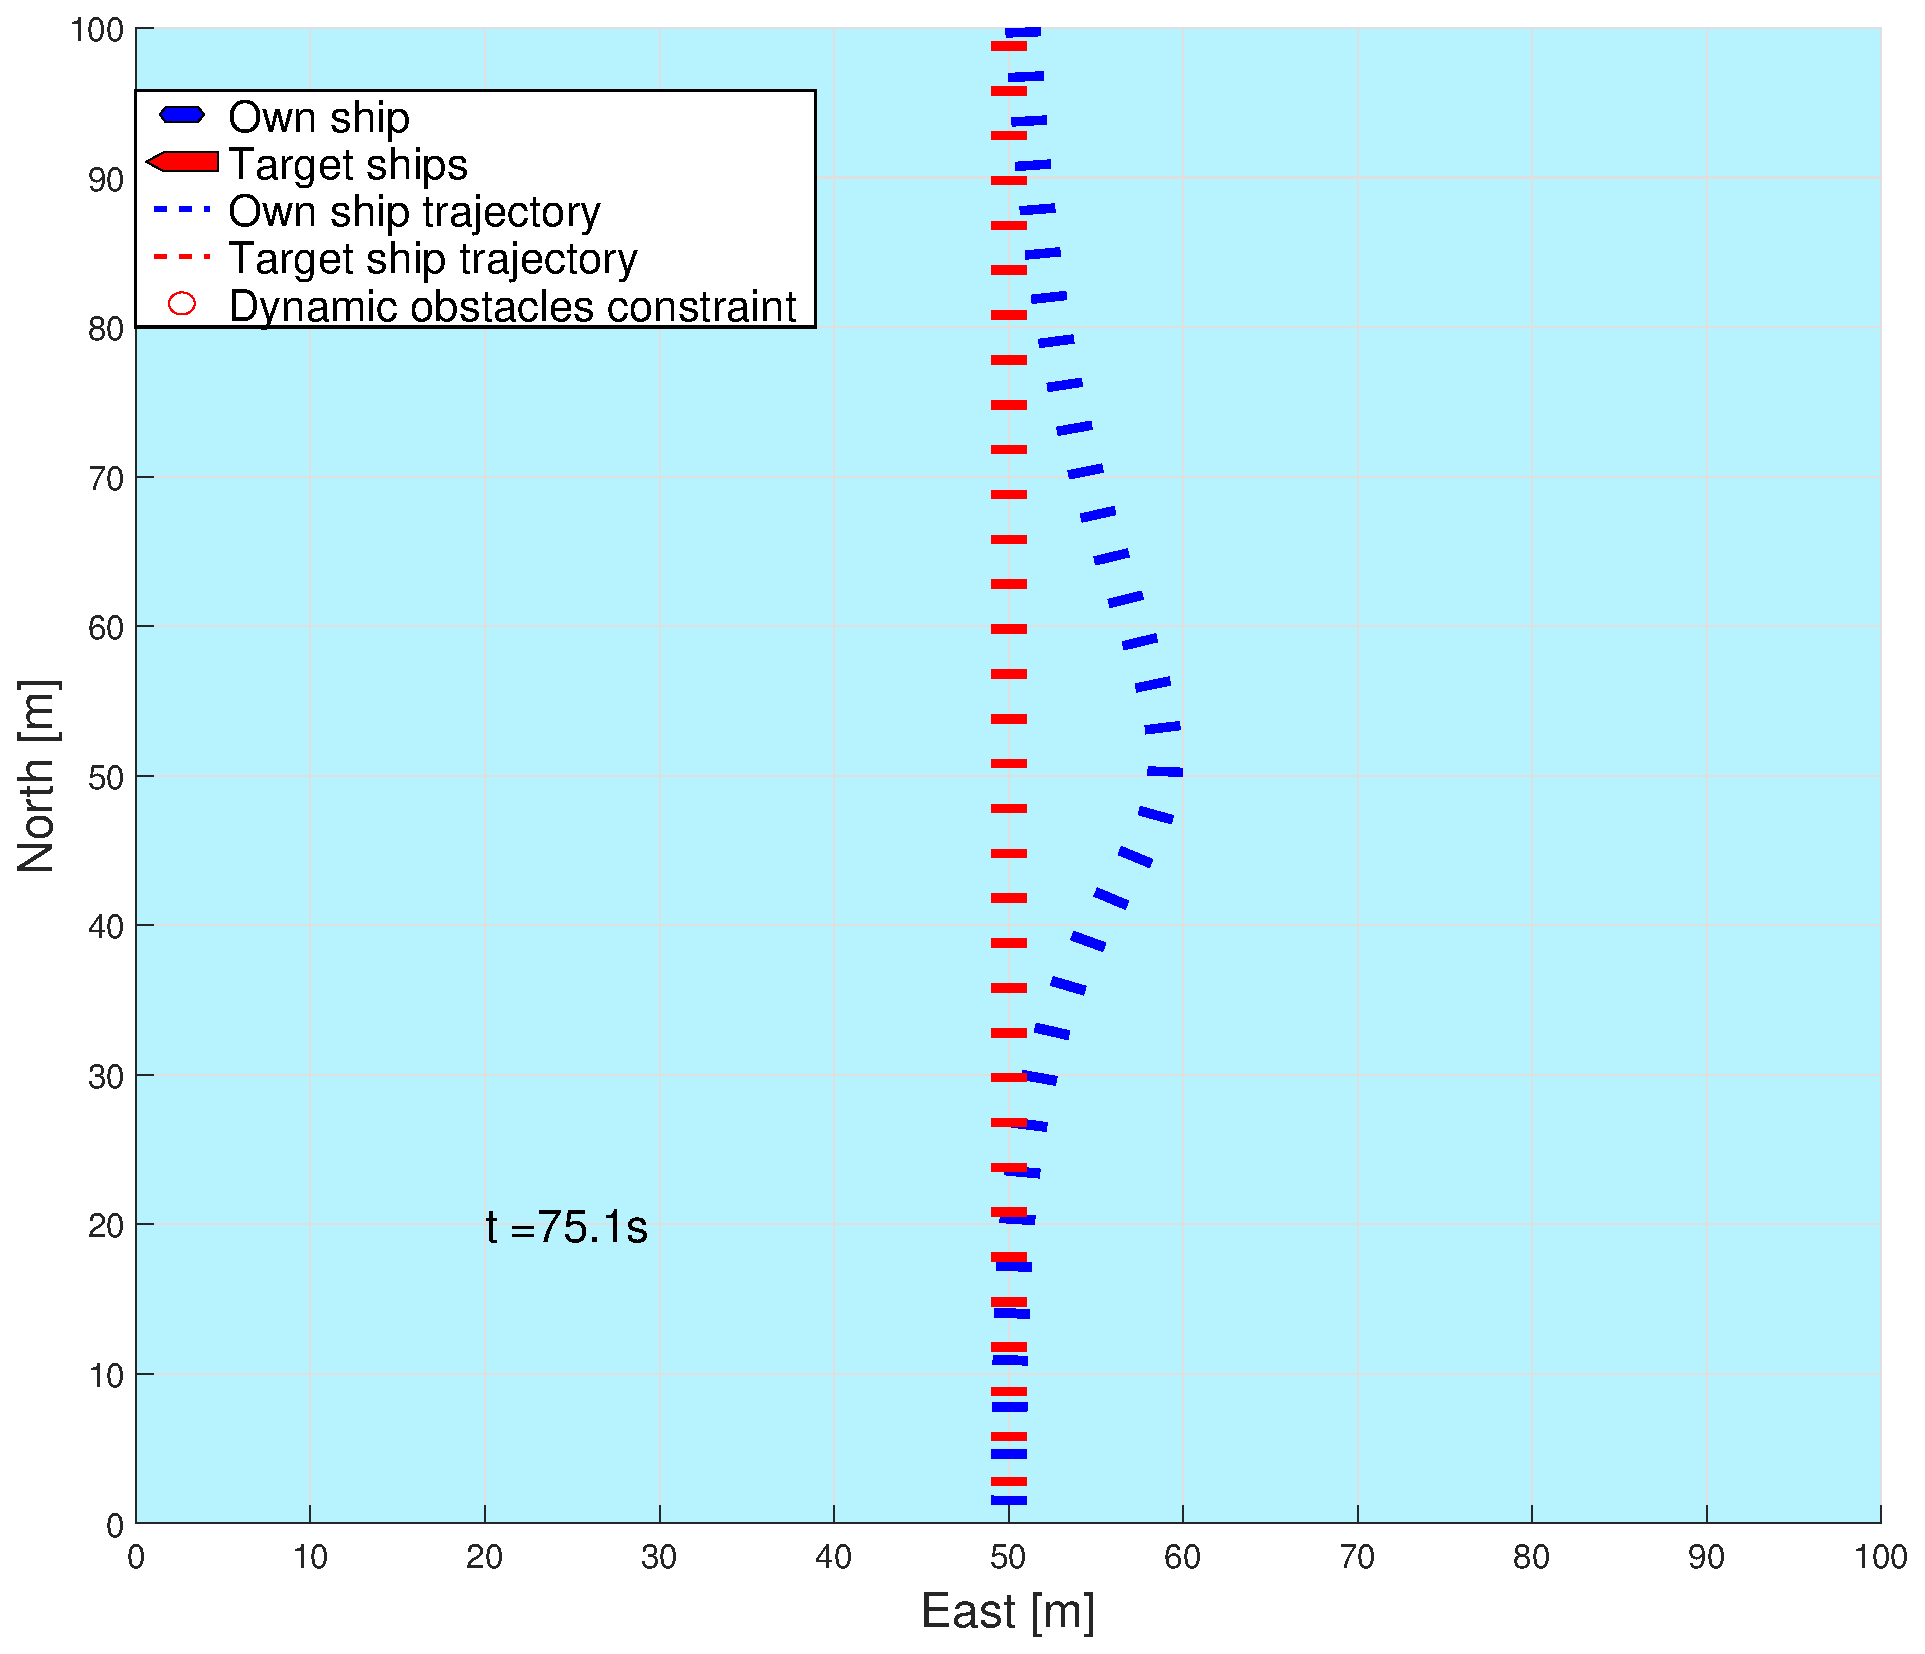
\includegraphics[width=\textwidth]{Images/Figures/enkel_HO/_Simple_0fig1_time=75}
        \subcaption{caption}
    \end{subfigure}
    \hfill
    \begin{subfigure}[b]{0.499\textwidth}
        \centering
        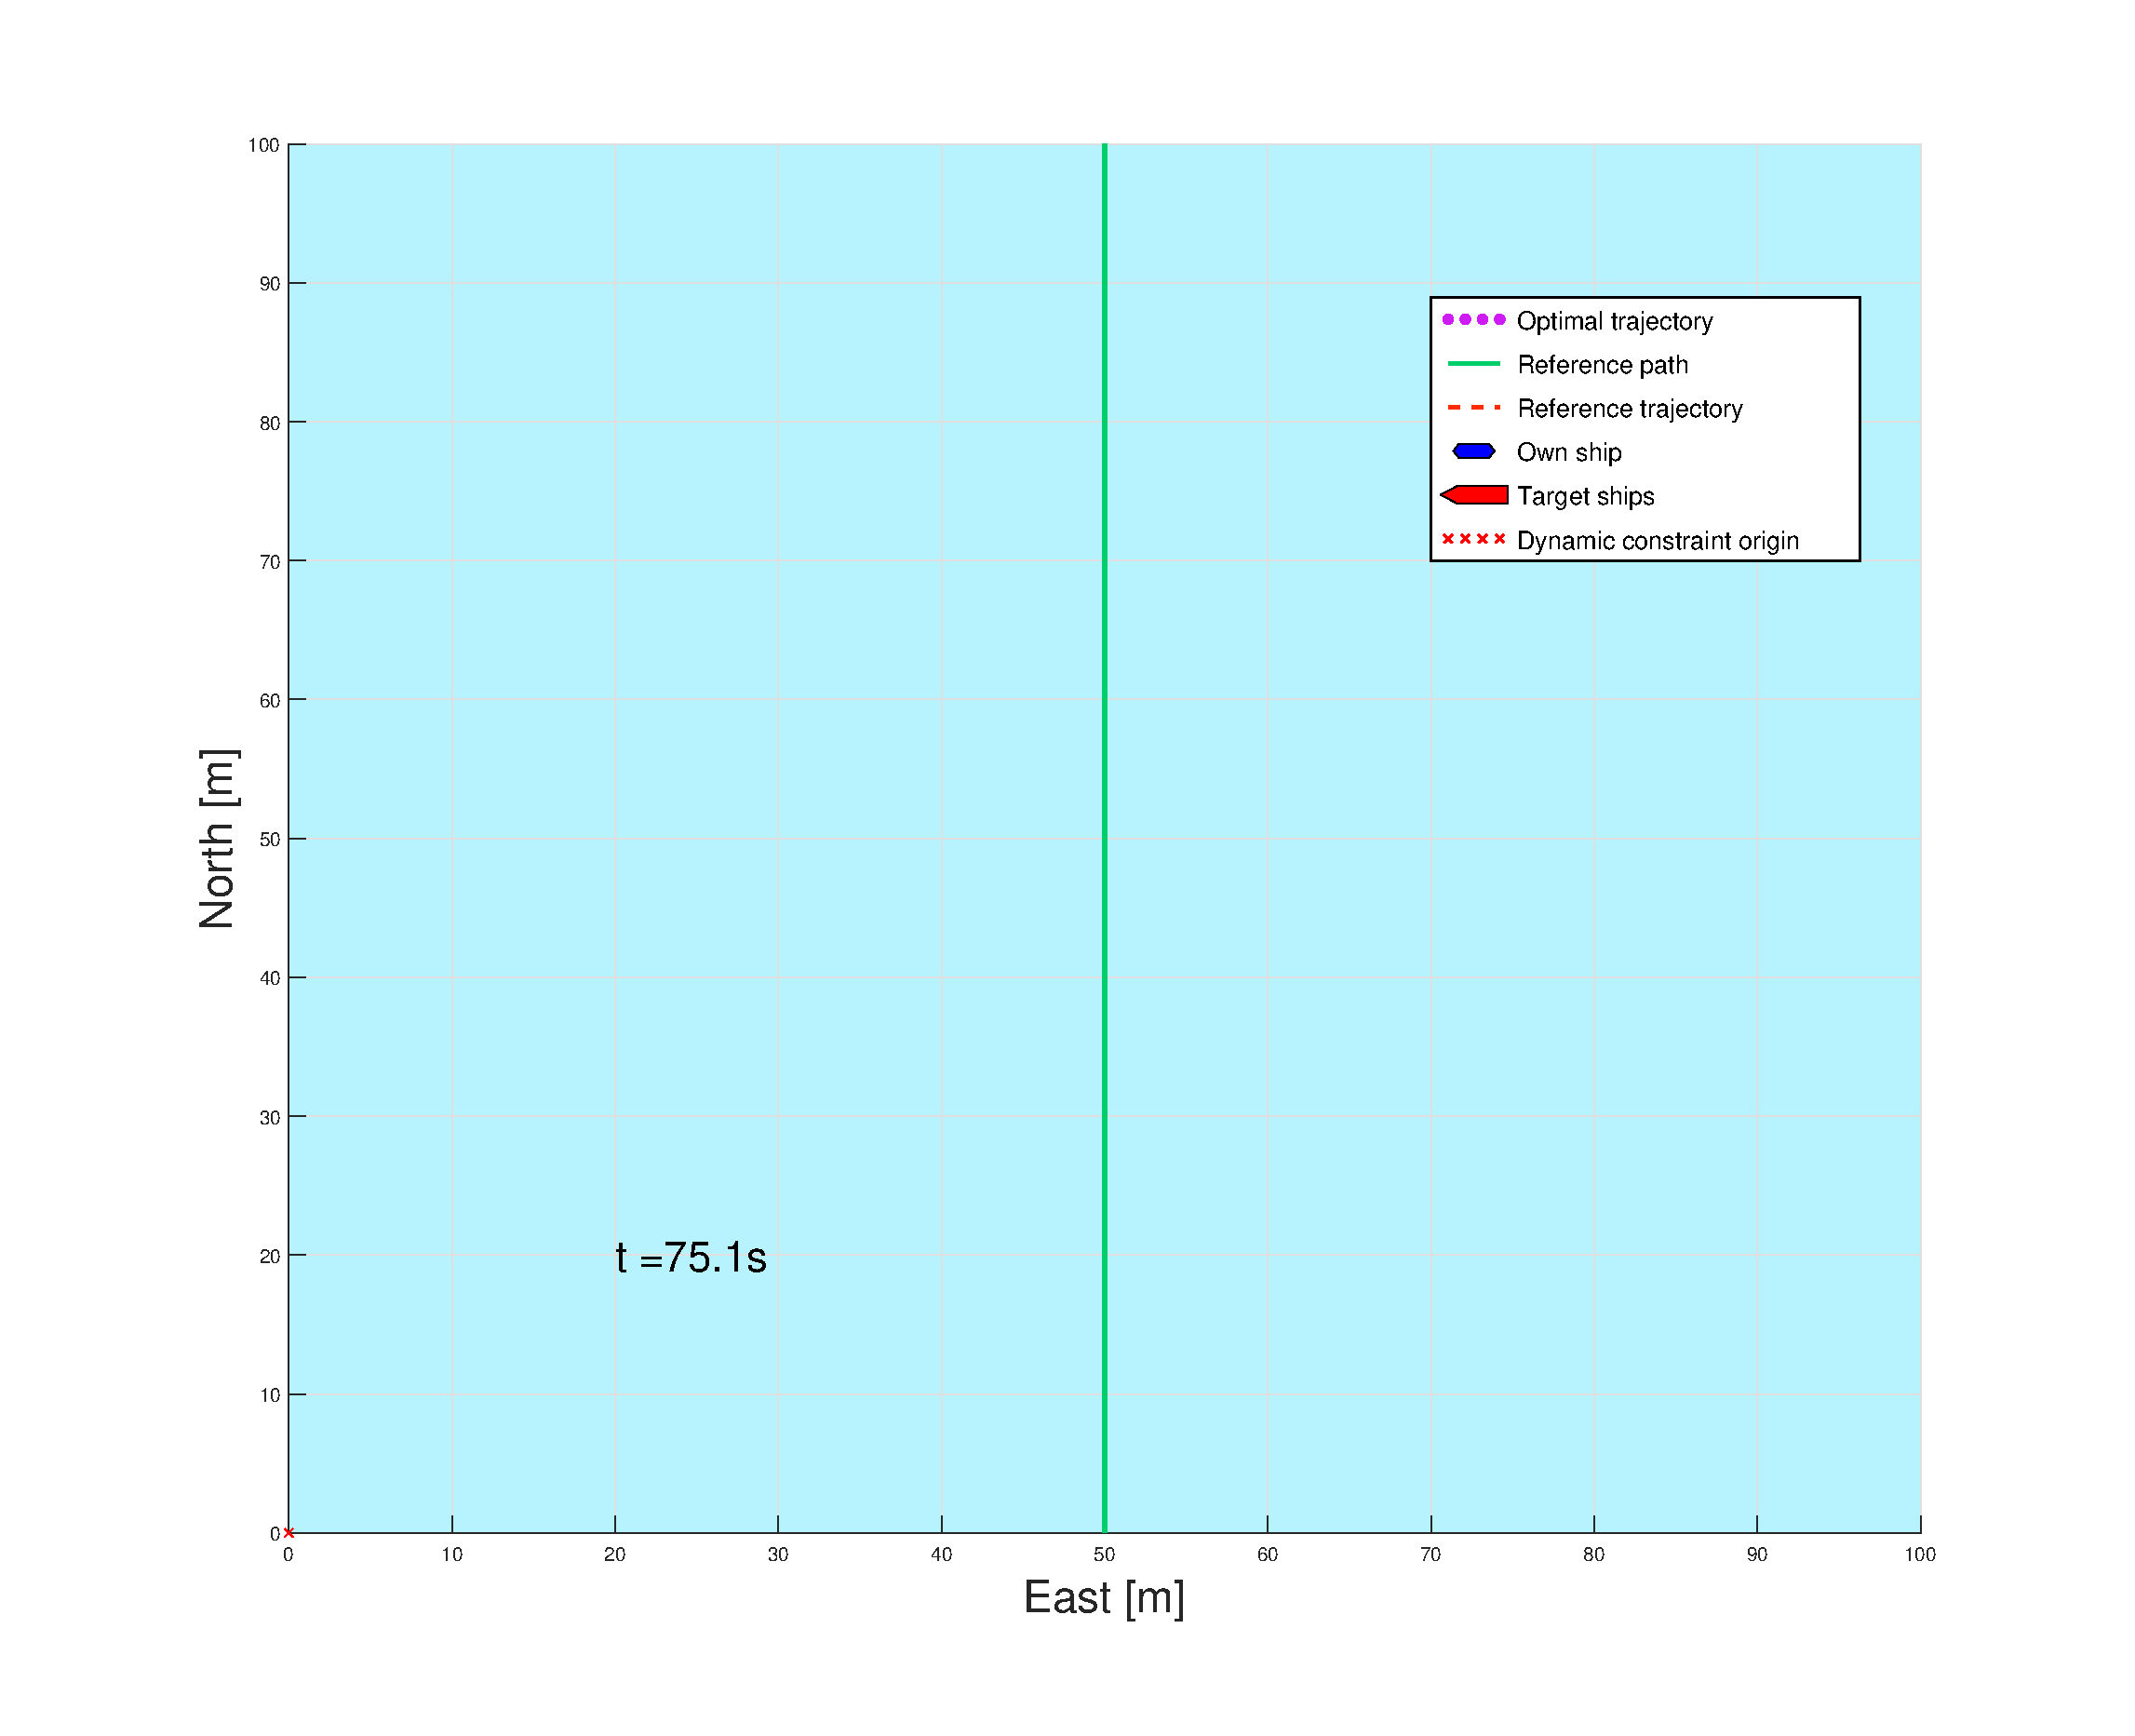
\includegraphics[width=\textwidth]{Images/Figures/enkel_HO/_Simple_0fig999_time=75}
        \subcaption{mhm}
    \end{subfigure}
    \hfill
    \caption{Simple Head on With Prediction}
\end{figure}

\begin{figure}[!b] %Canals simulation, shown with and without constraints
    \begin{subfigure}[b]{0.49\textwidth}
        \centering
        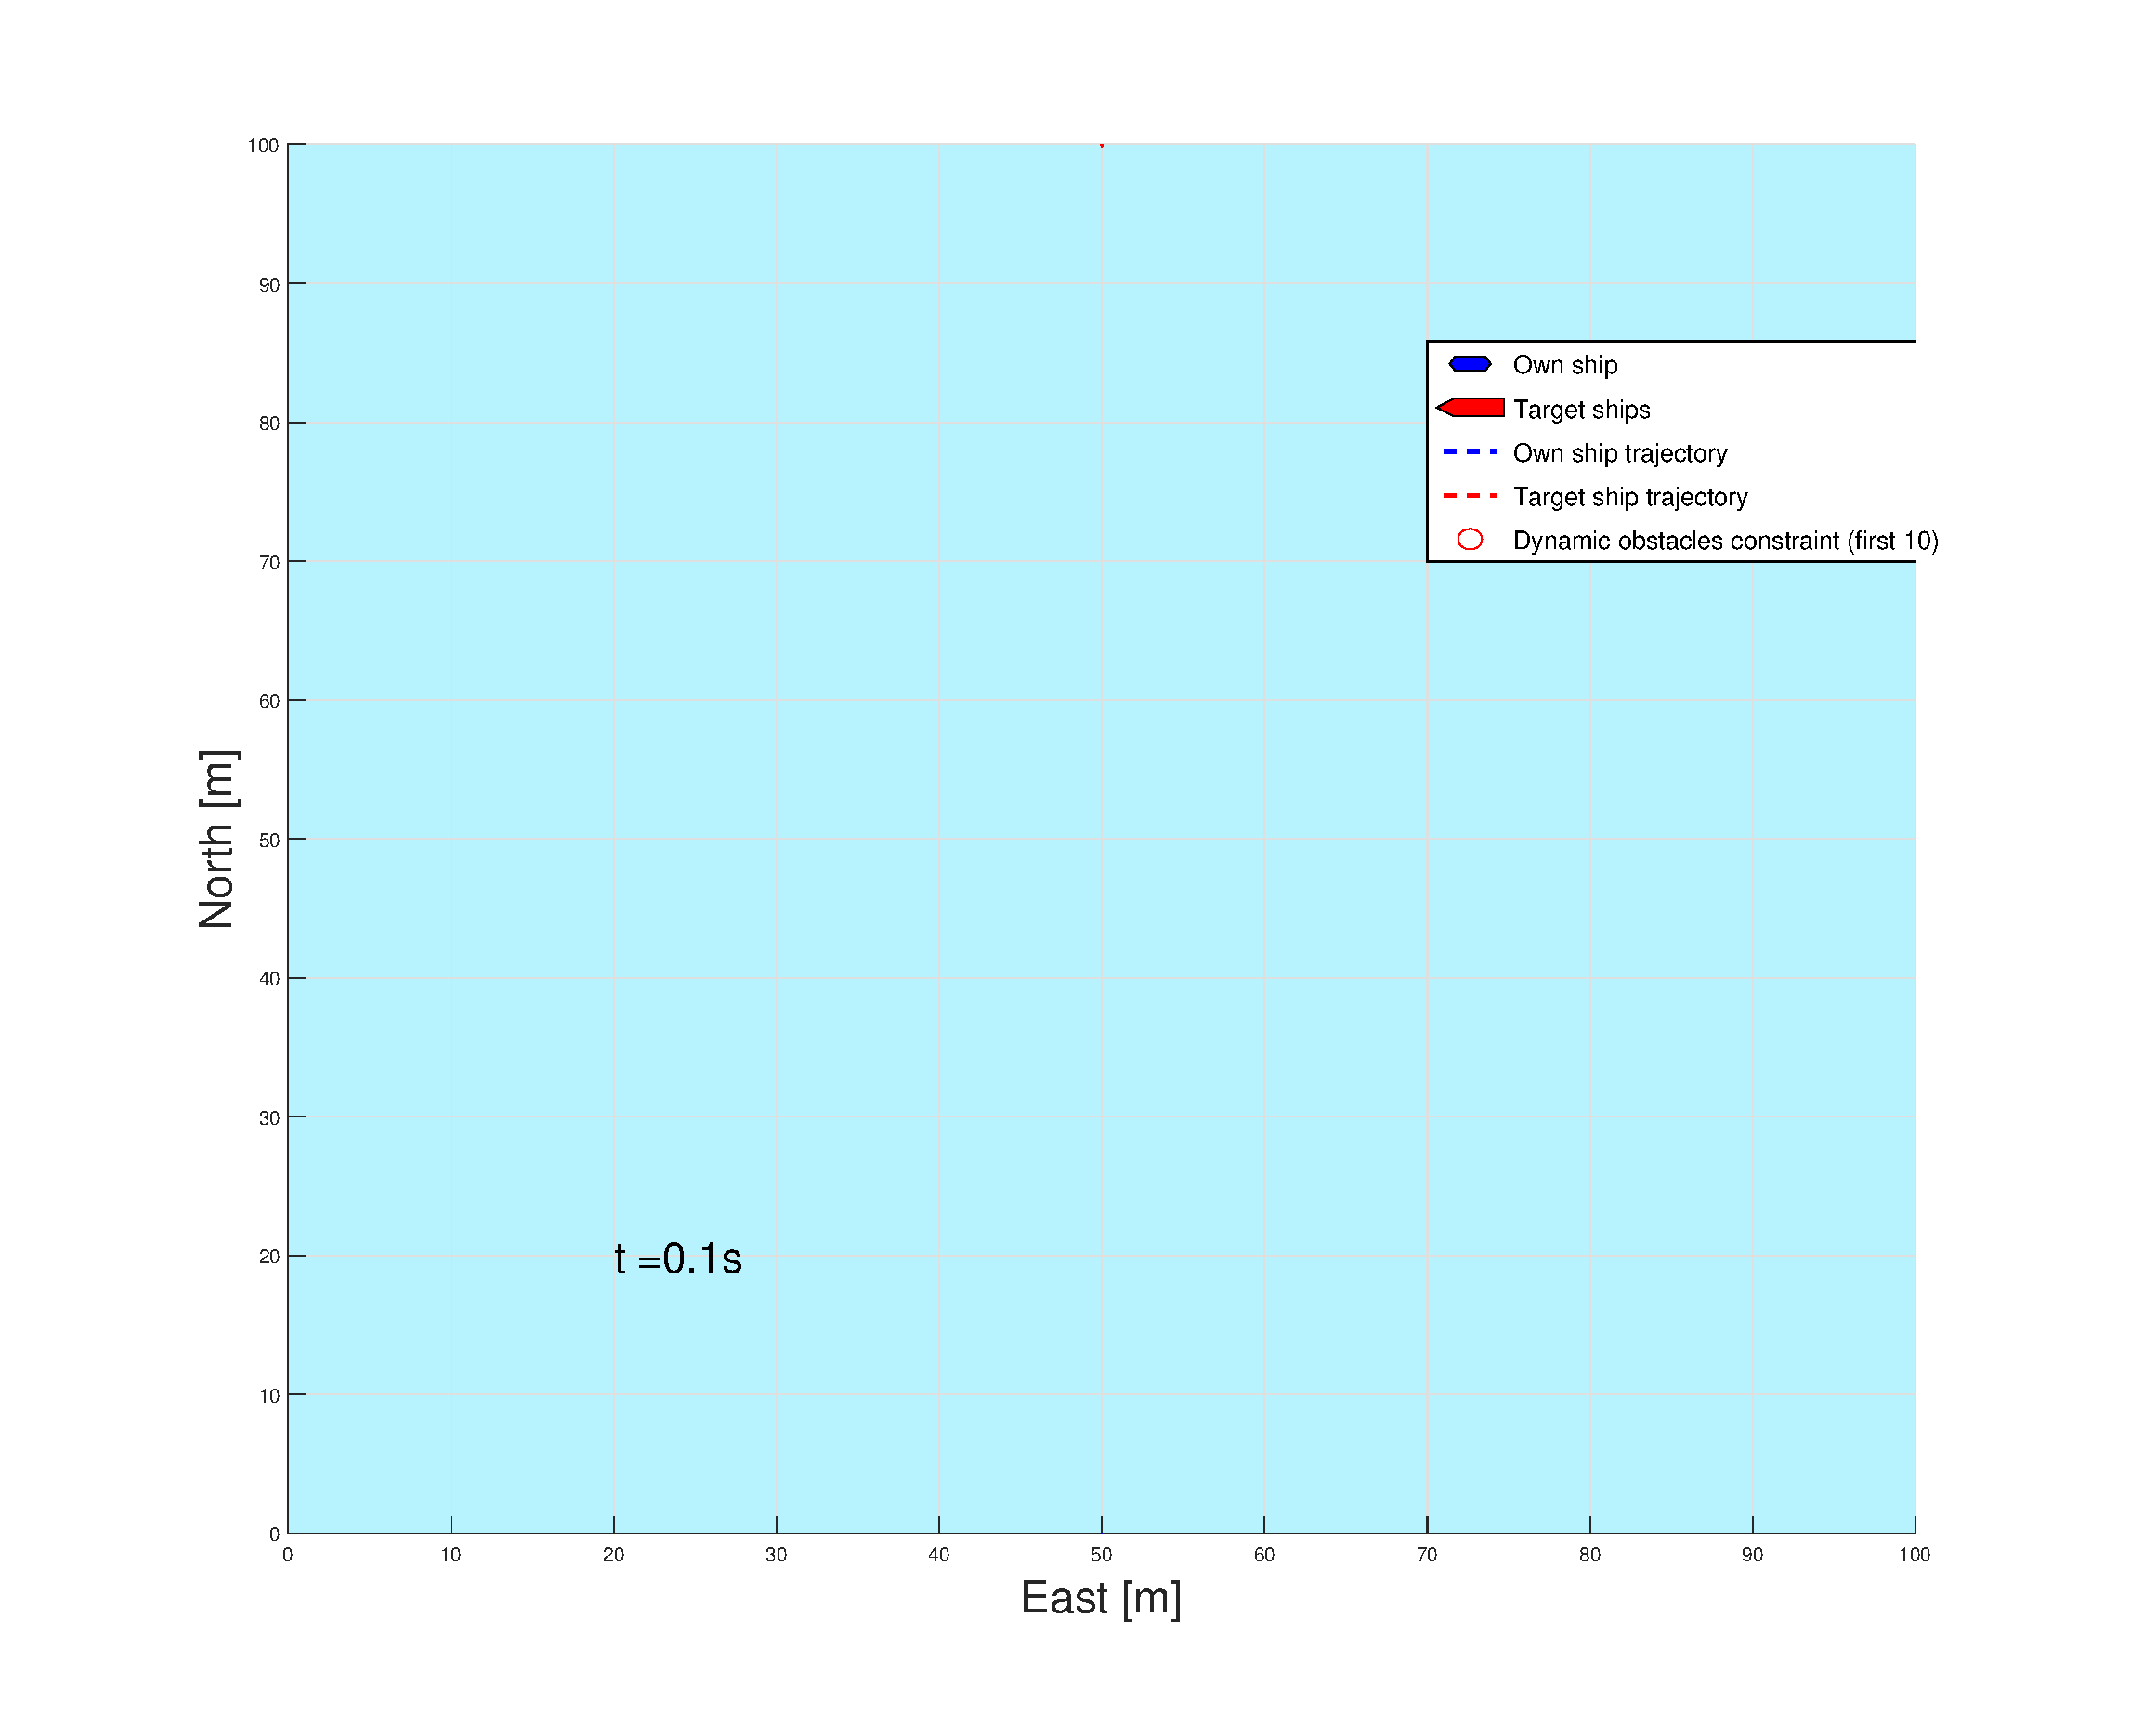
\includegraphics[width=\textwidth]{Images/Figures/enkel_HO/_Simple_1fig1_time=0}
        \subcaption{caption}
    \end{subfigure}
    \hfill
    \begin{subfigure}[b]{0.499\textwidth}
        \centering
        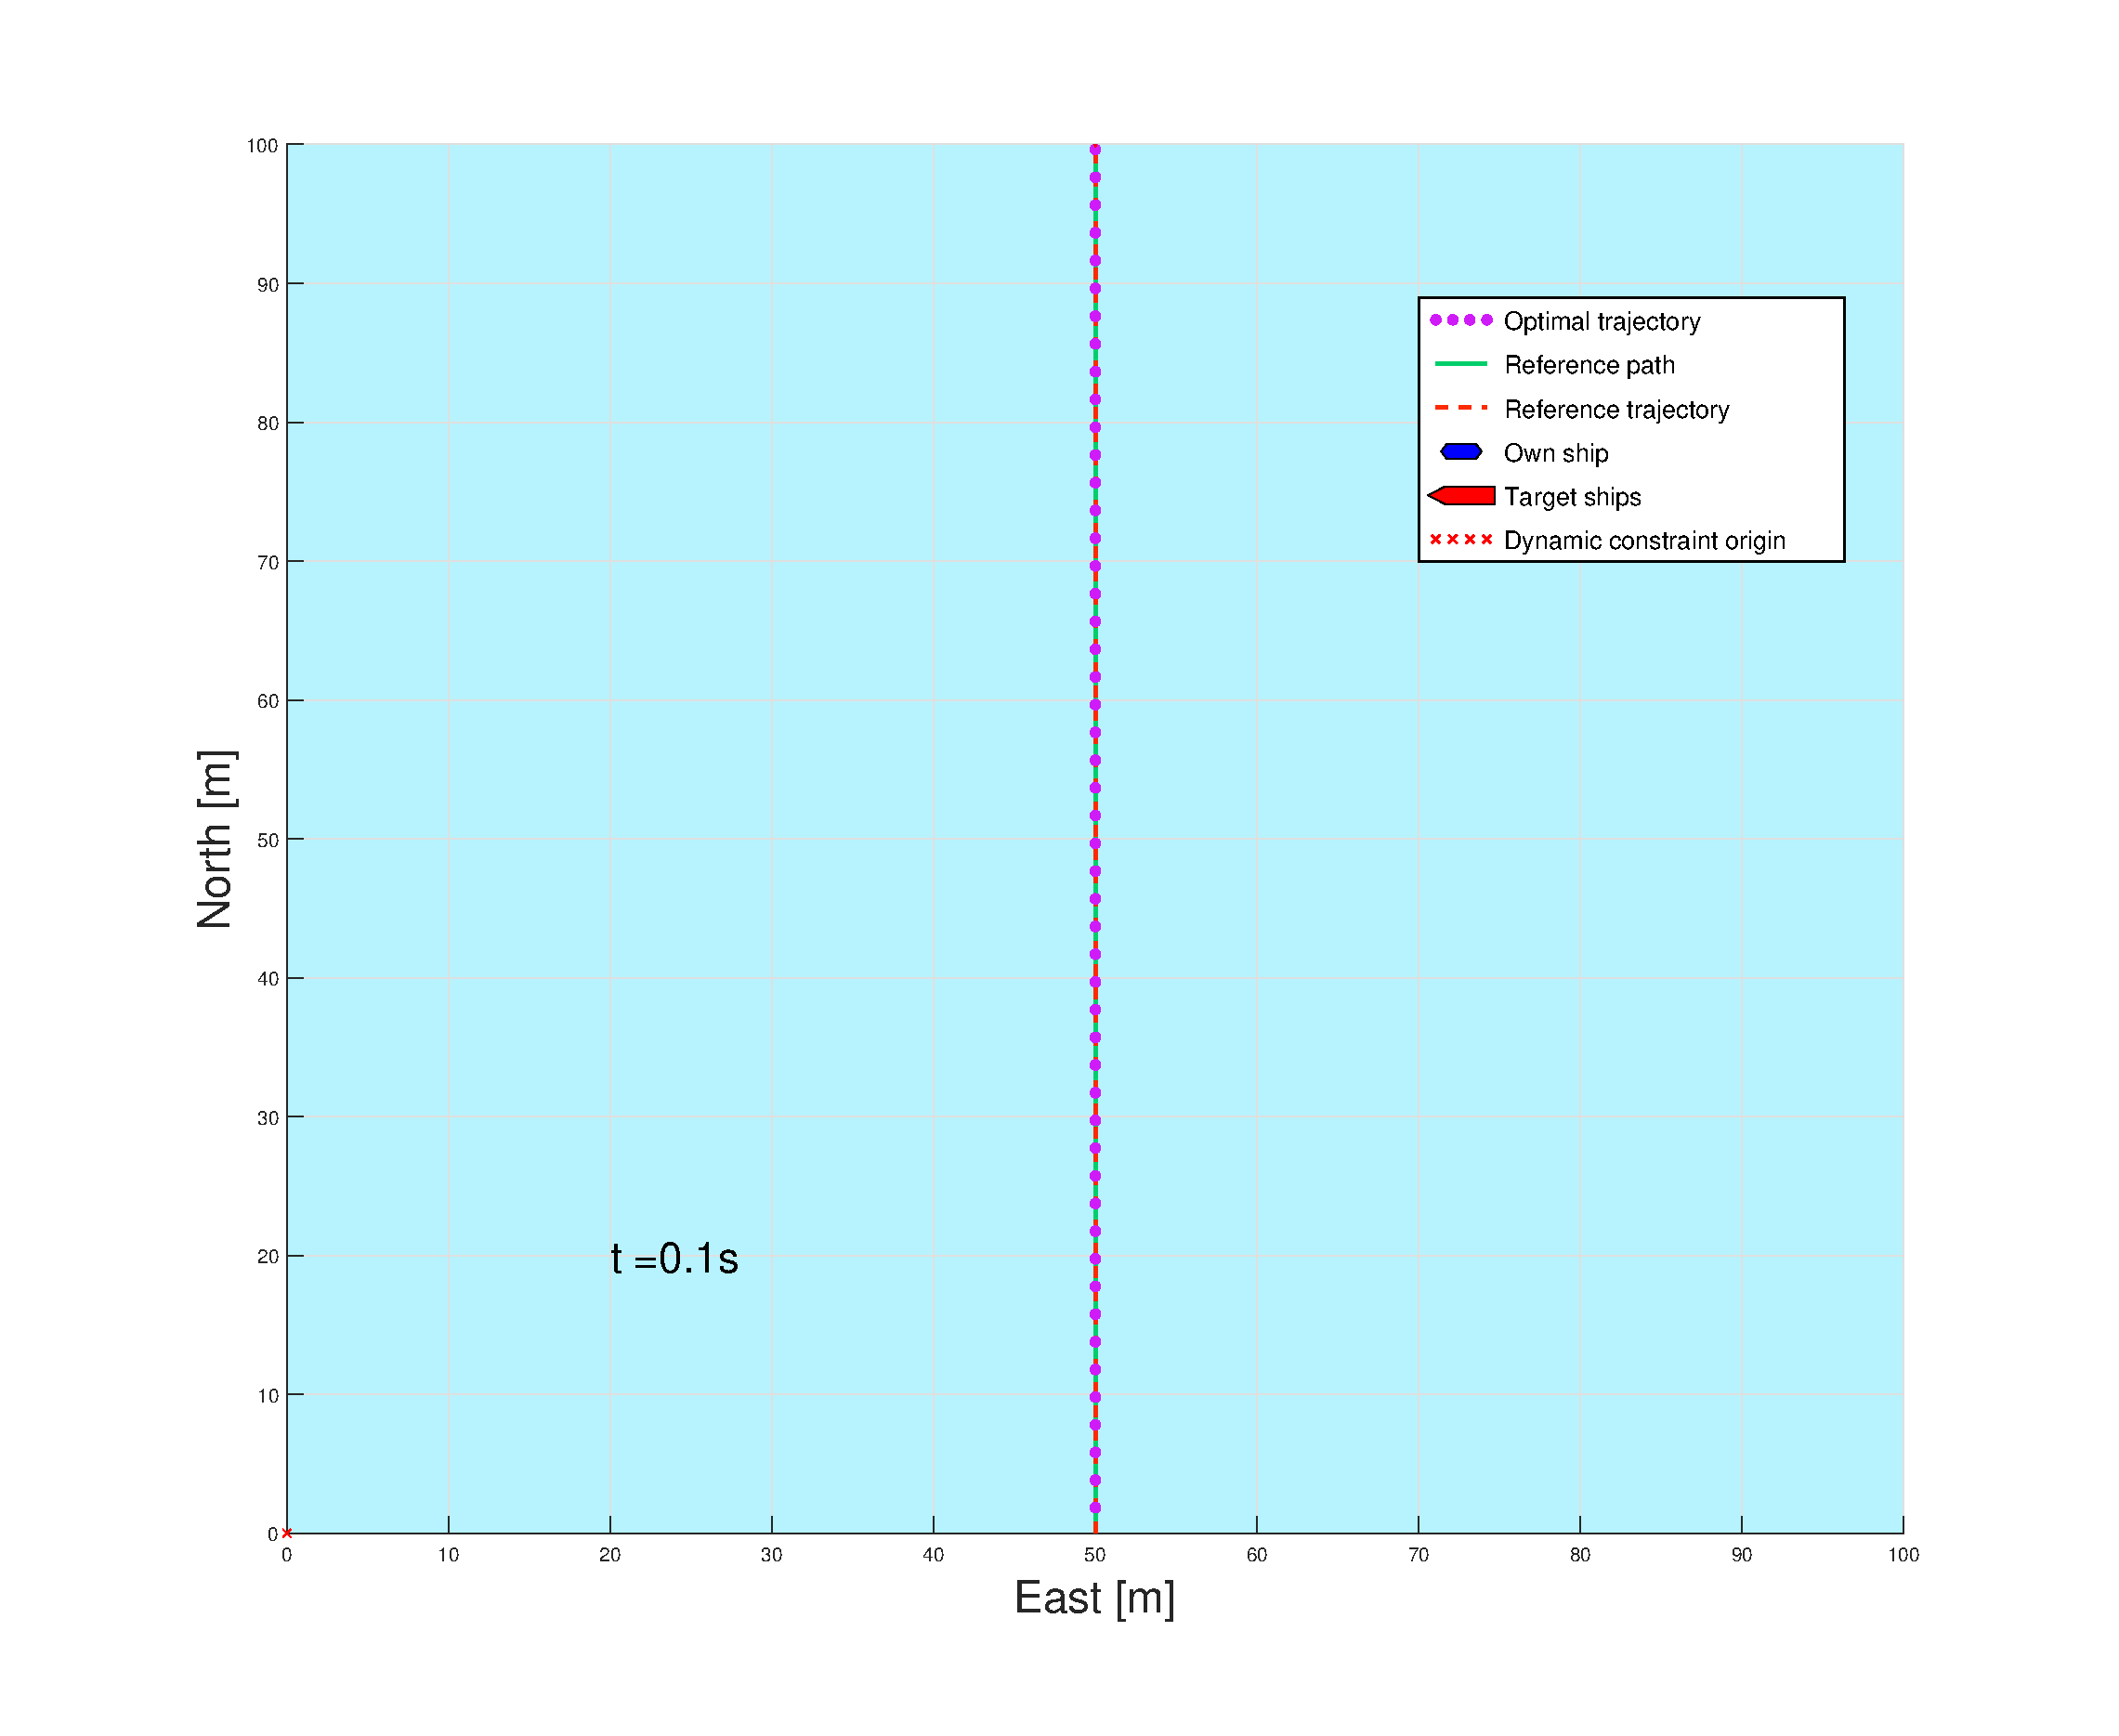
\includegraphics[width=\textwidth]{Images/Figures/enkel_HO/_Simple_1fig999_time=0}
        \subcaption{mhm}
    \end{subfigure}
    \hfill
    \\
    \begin{subfigure}[b]{0.49\textwidth}
        \centering
        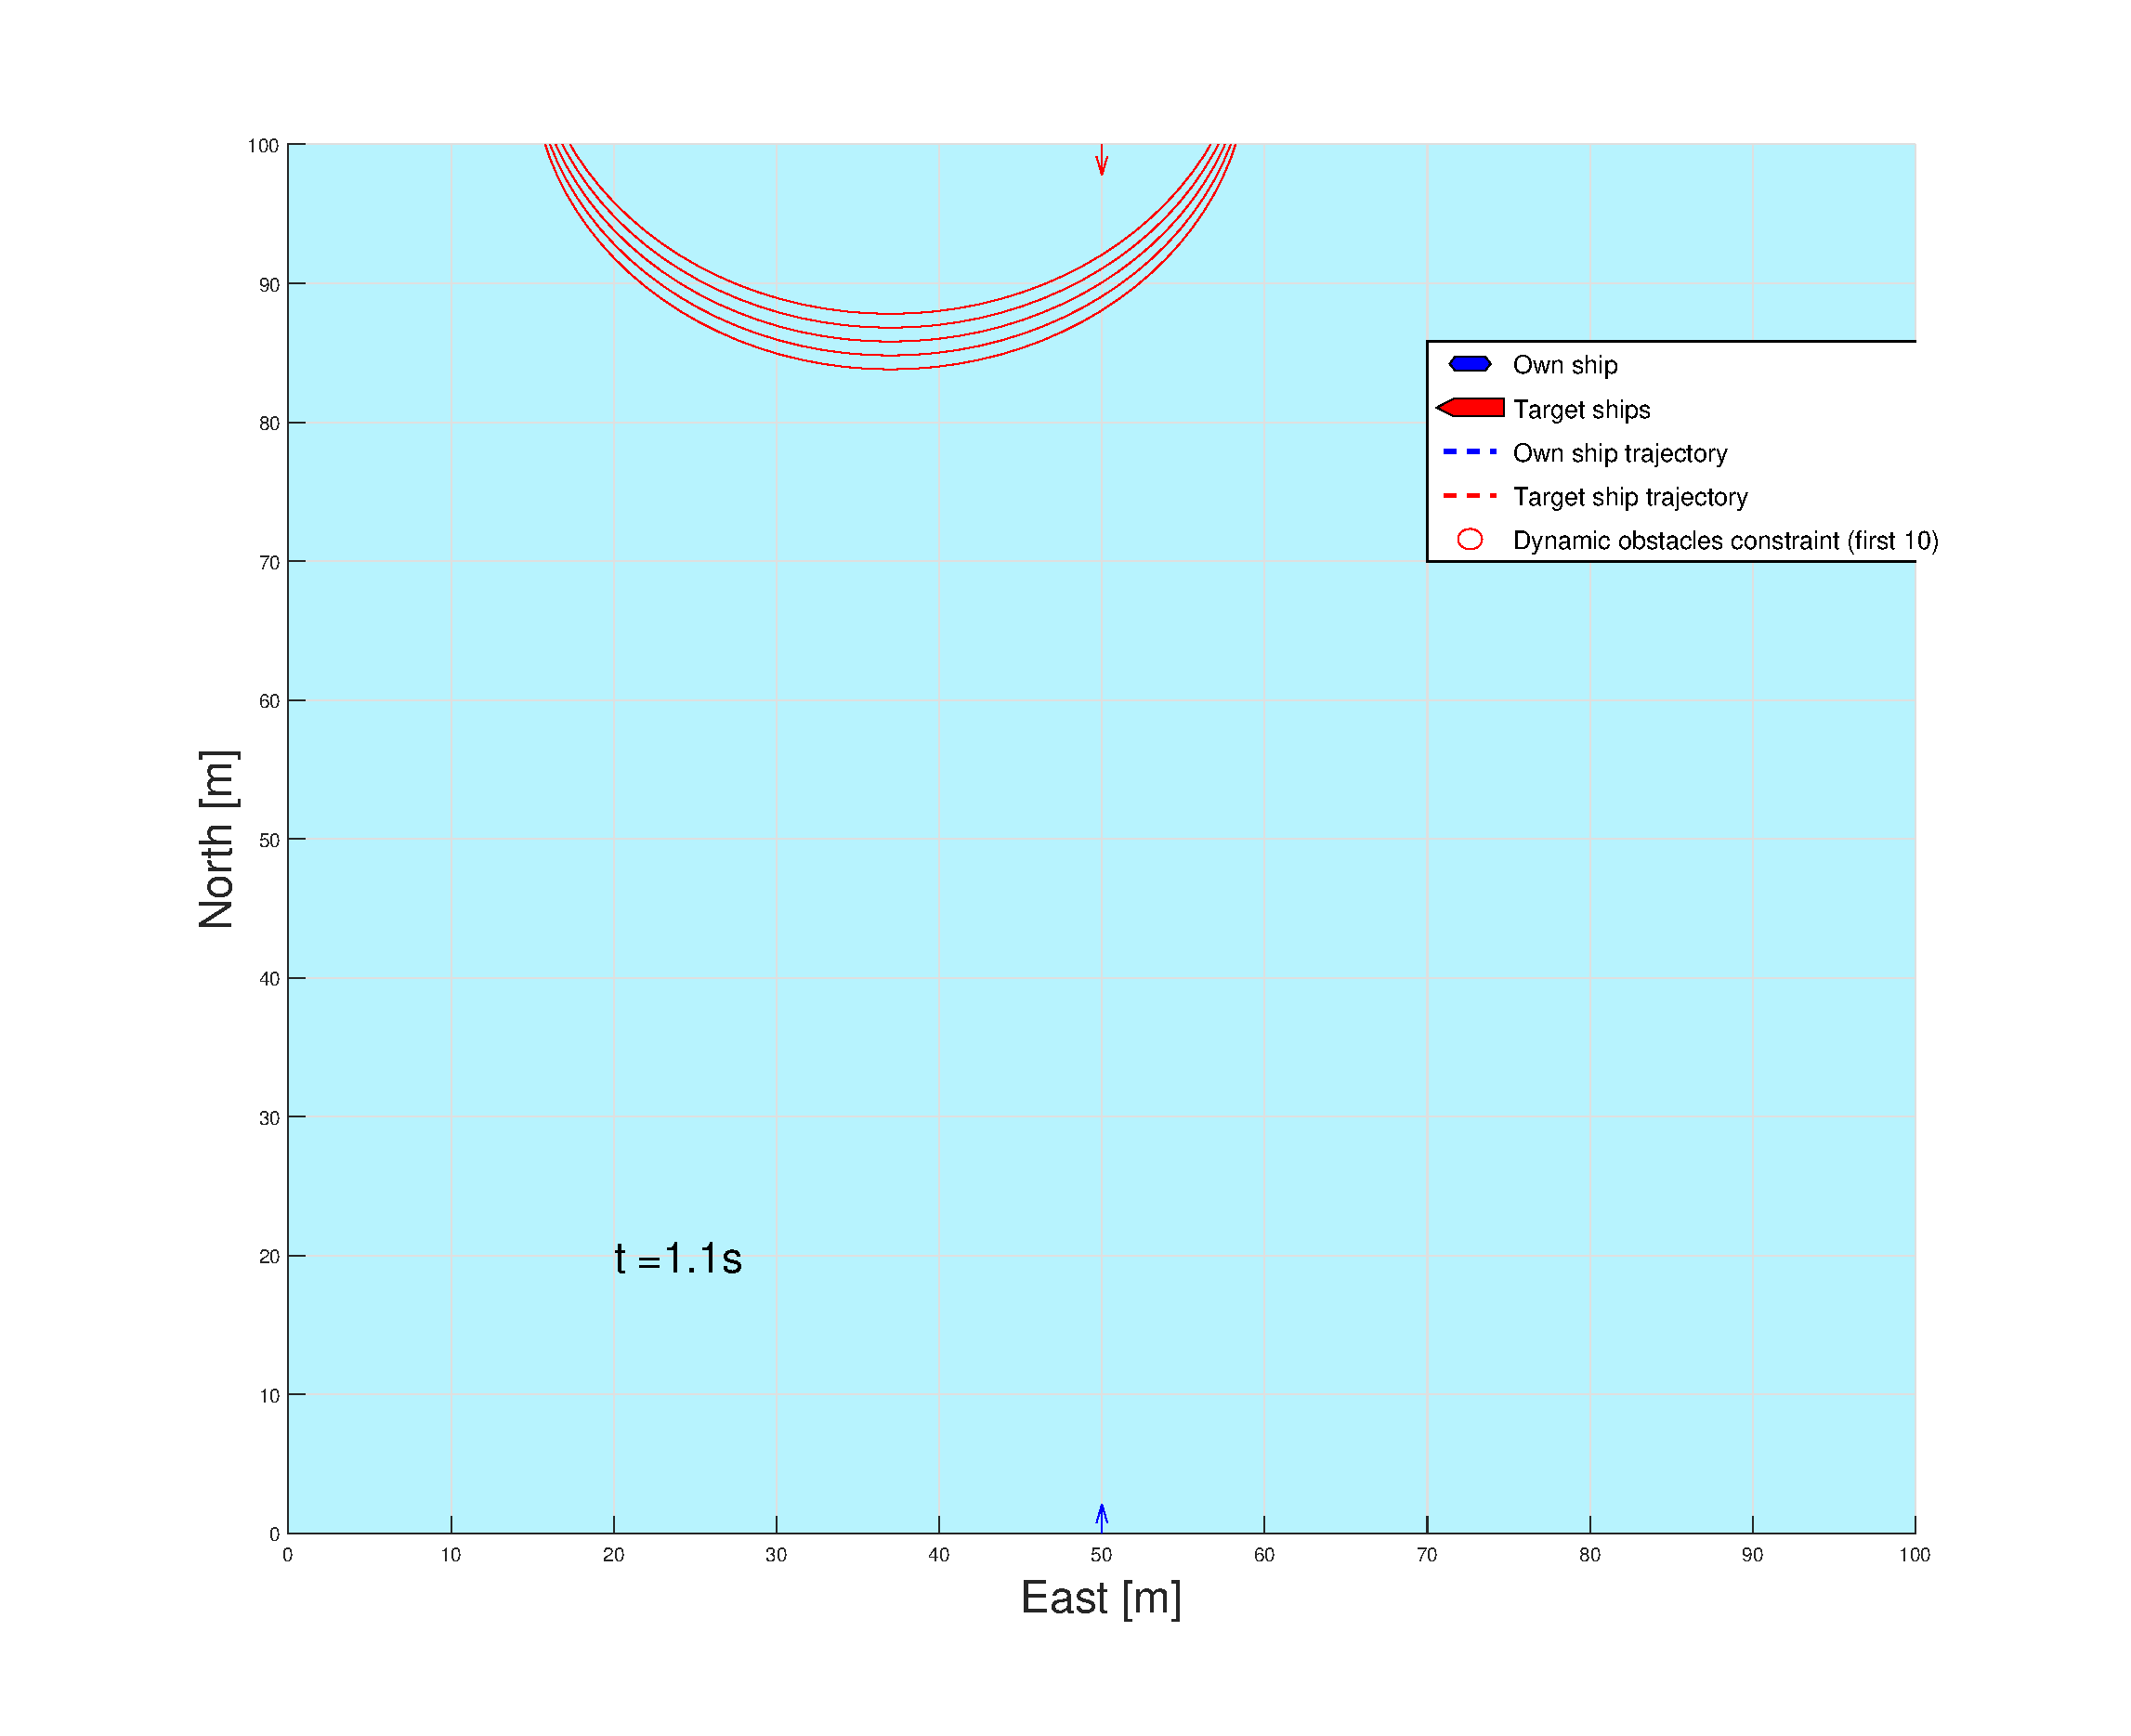
\includegraphics[width=\textwidth]{Images/Figures/enkel_HO/_Simple_1fig1_time=1}
        \subcaption{caption}
    \end{subfigure}
    \hfill
    \begin{subfigure}[b]{0.499\textwidth}
        \centering
        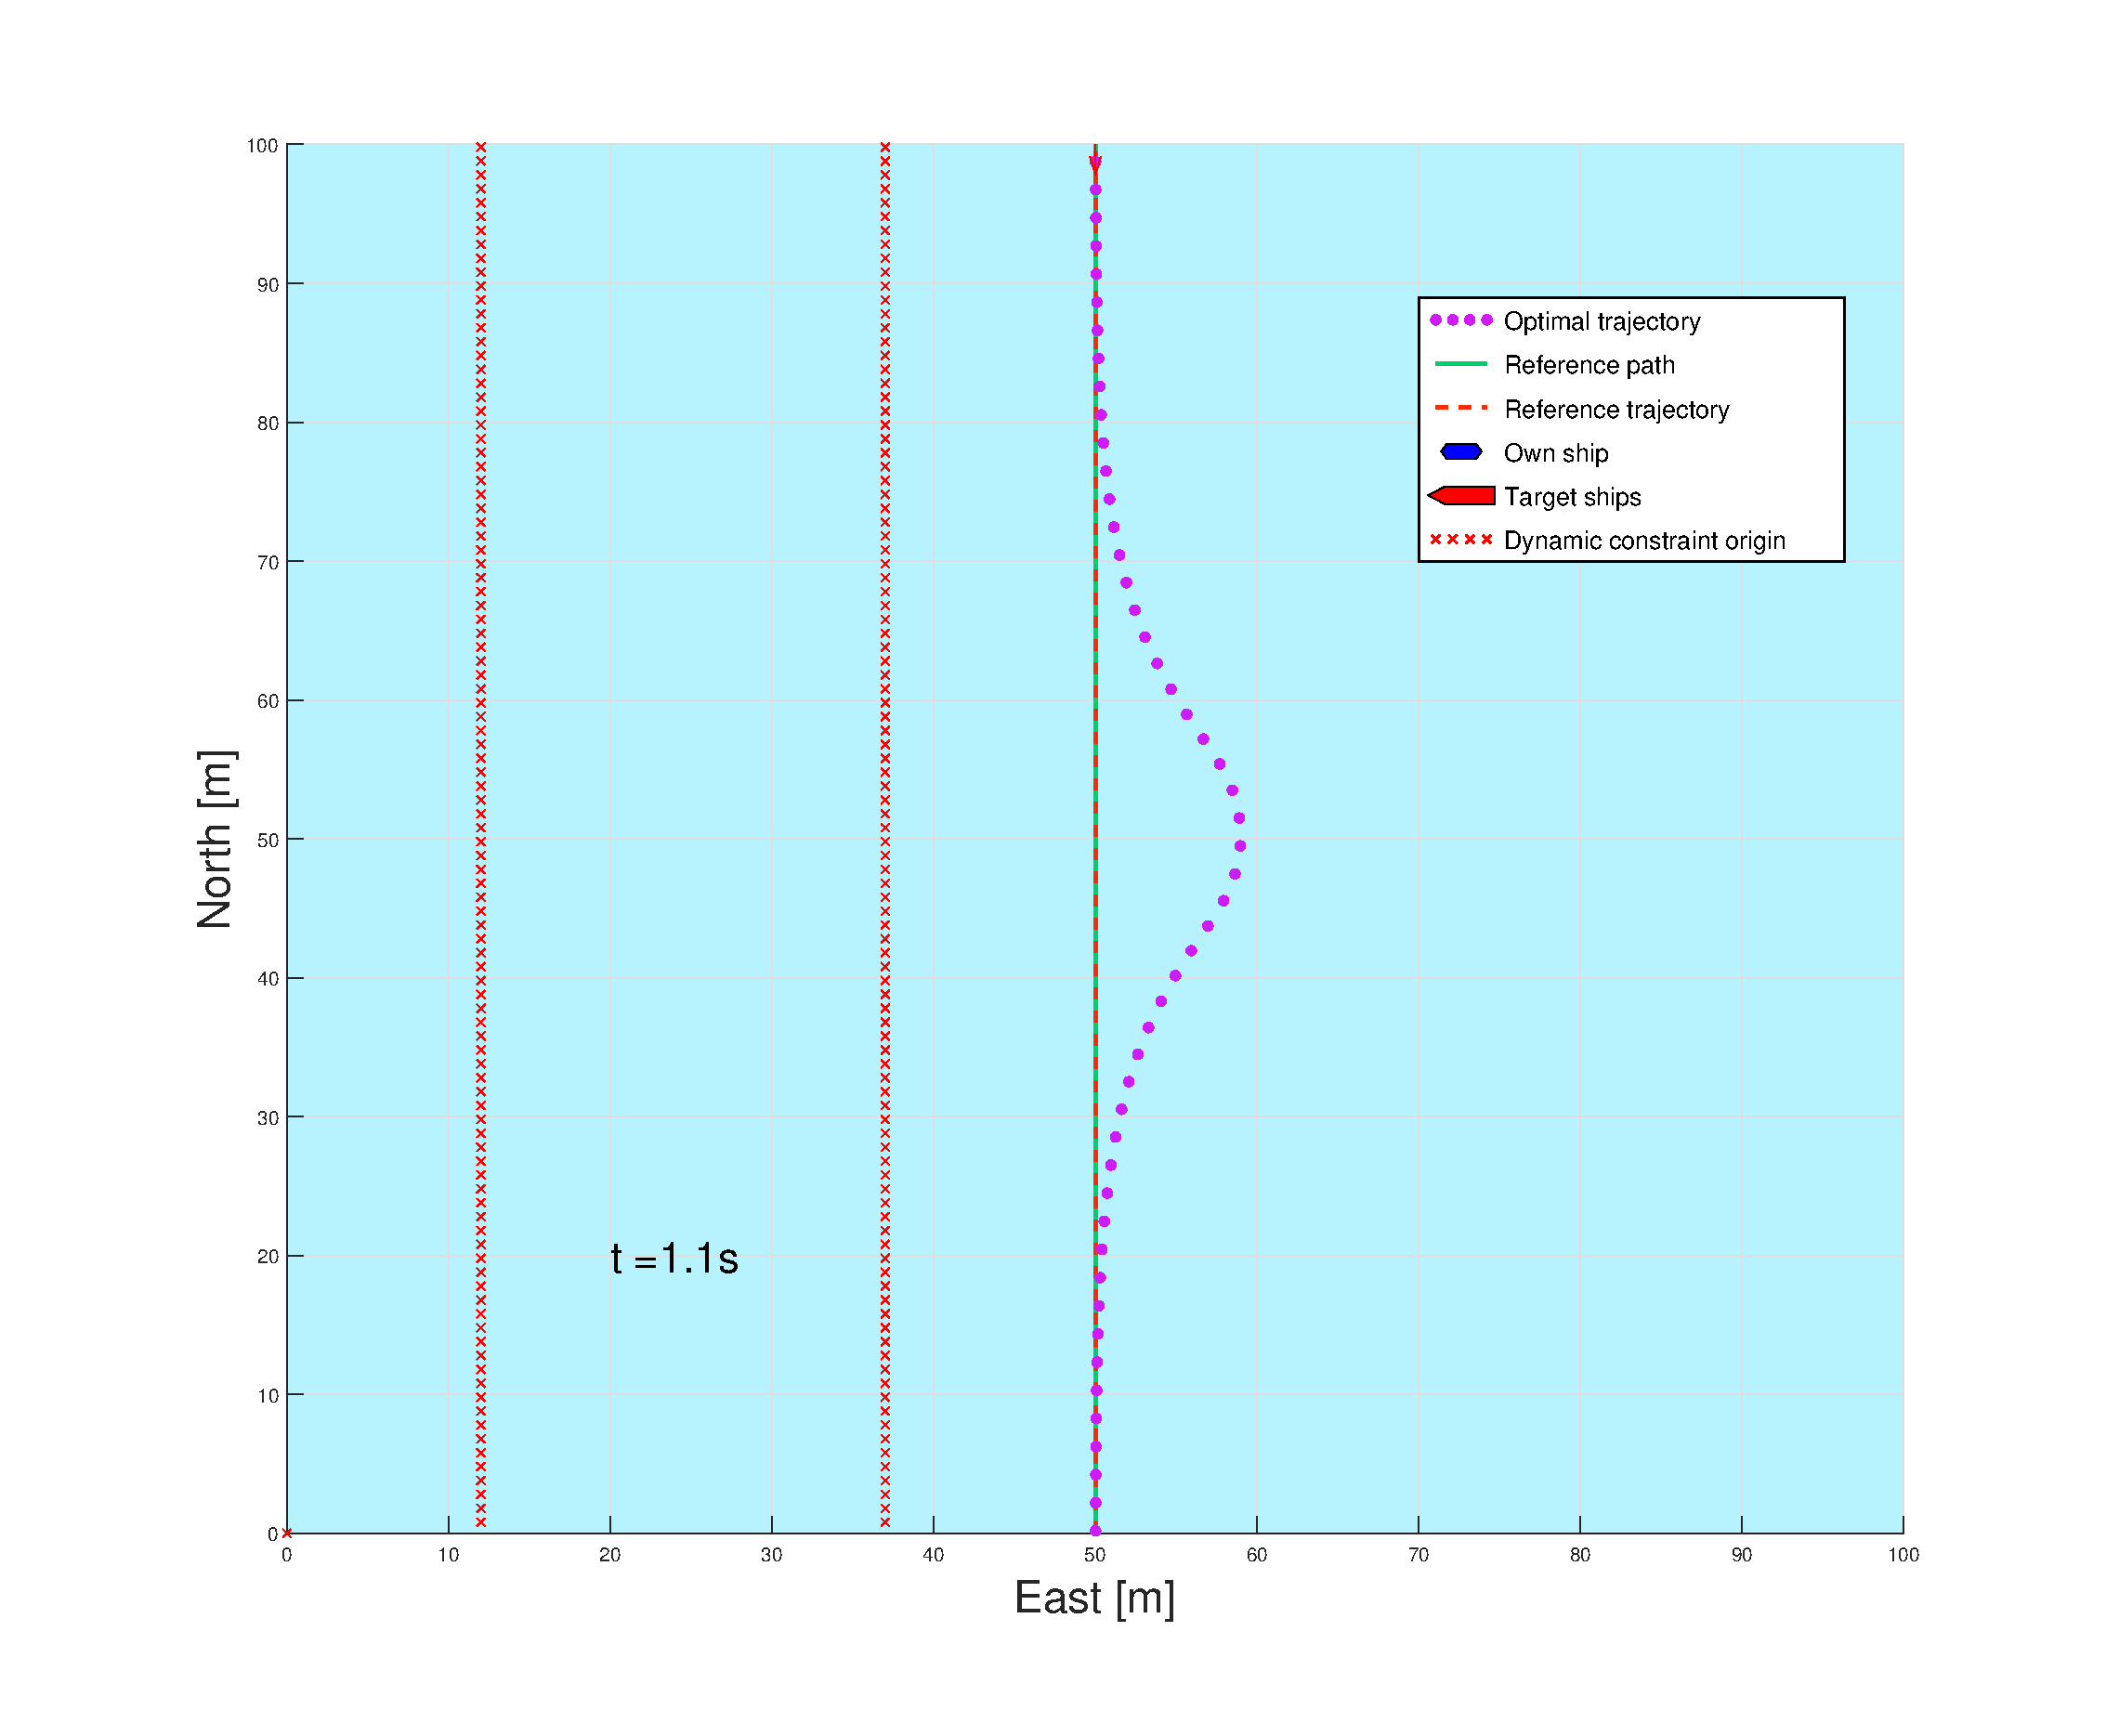
\includegraphics[width=\textwidth]{Images/Figures/enkel_HO/_Simple_1fig999_time=1}
        \subcaption{mhm}
    \end{subfigure}
    \hfill
    \\
    \begin{subfigure}[b]{0.49\textwidth}
        \centering
        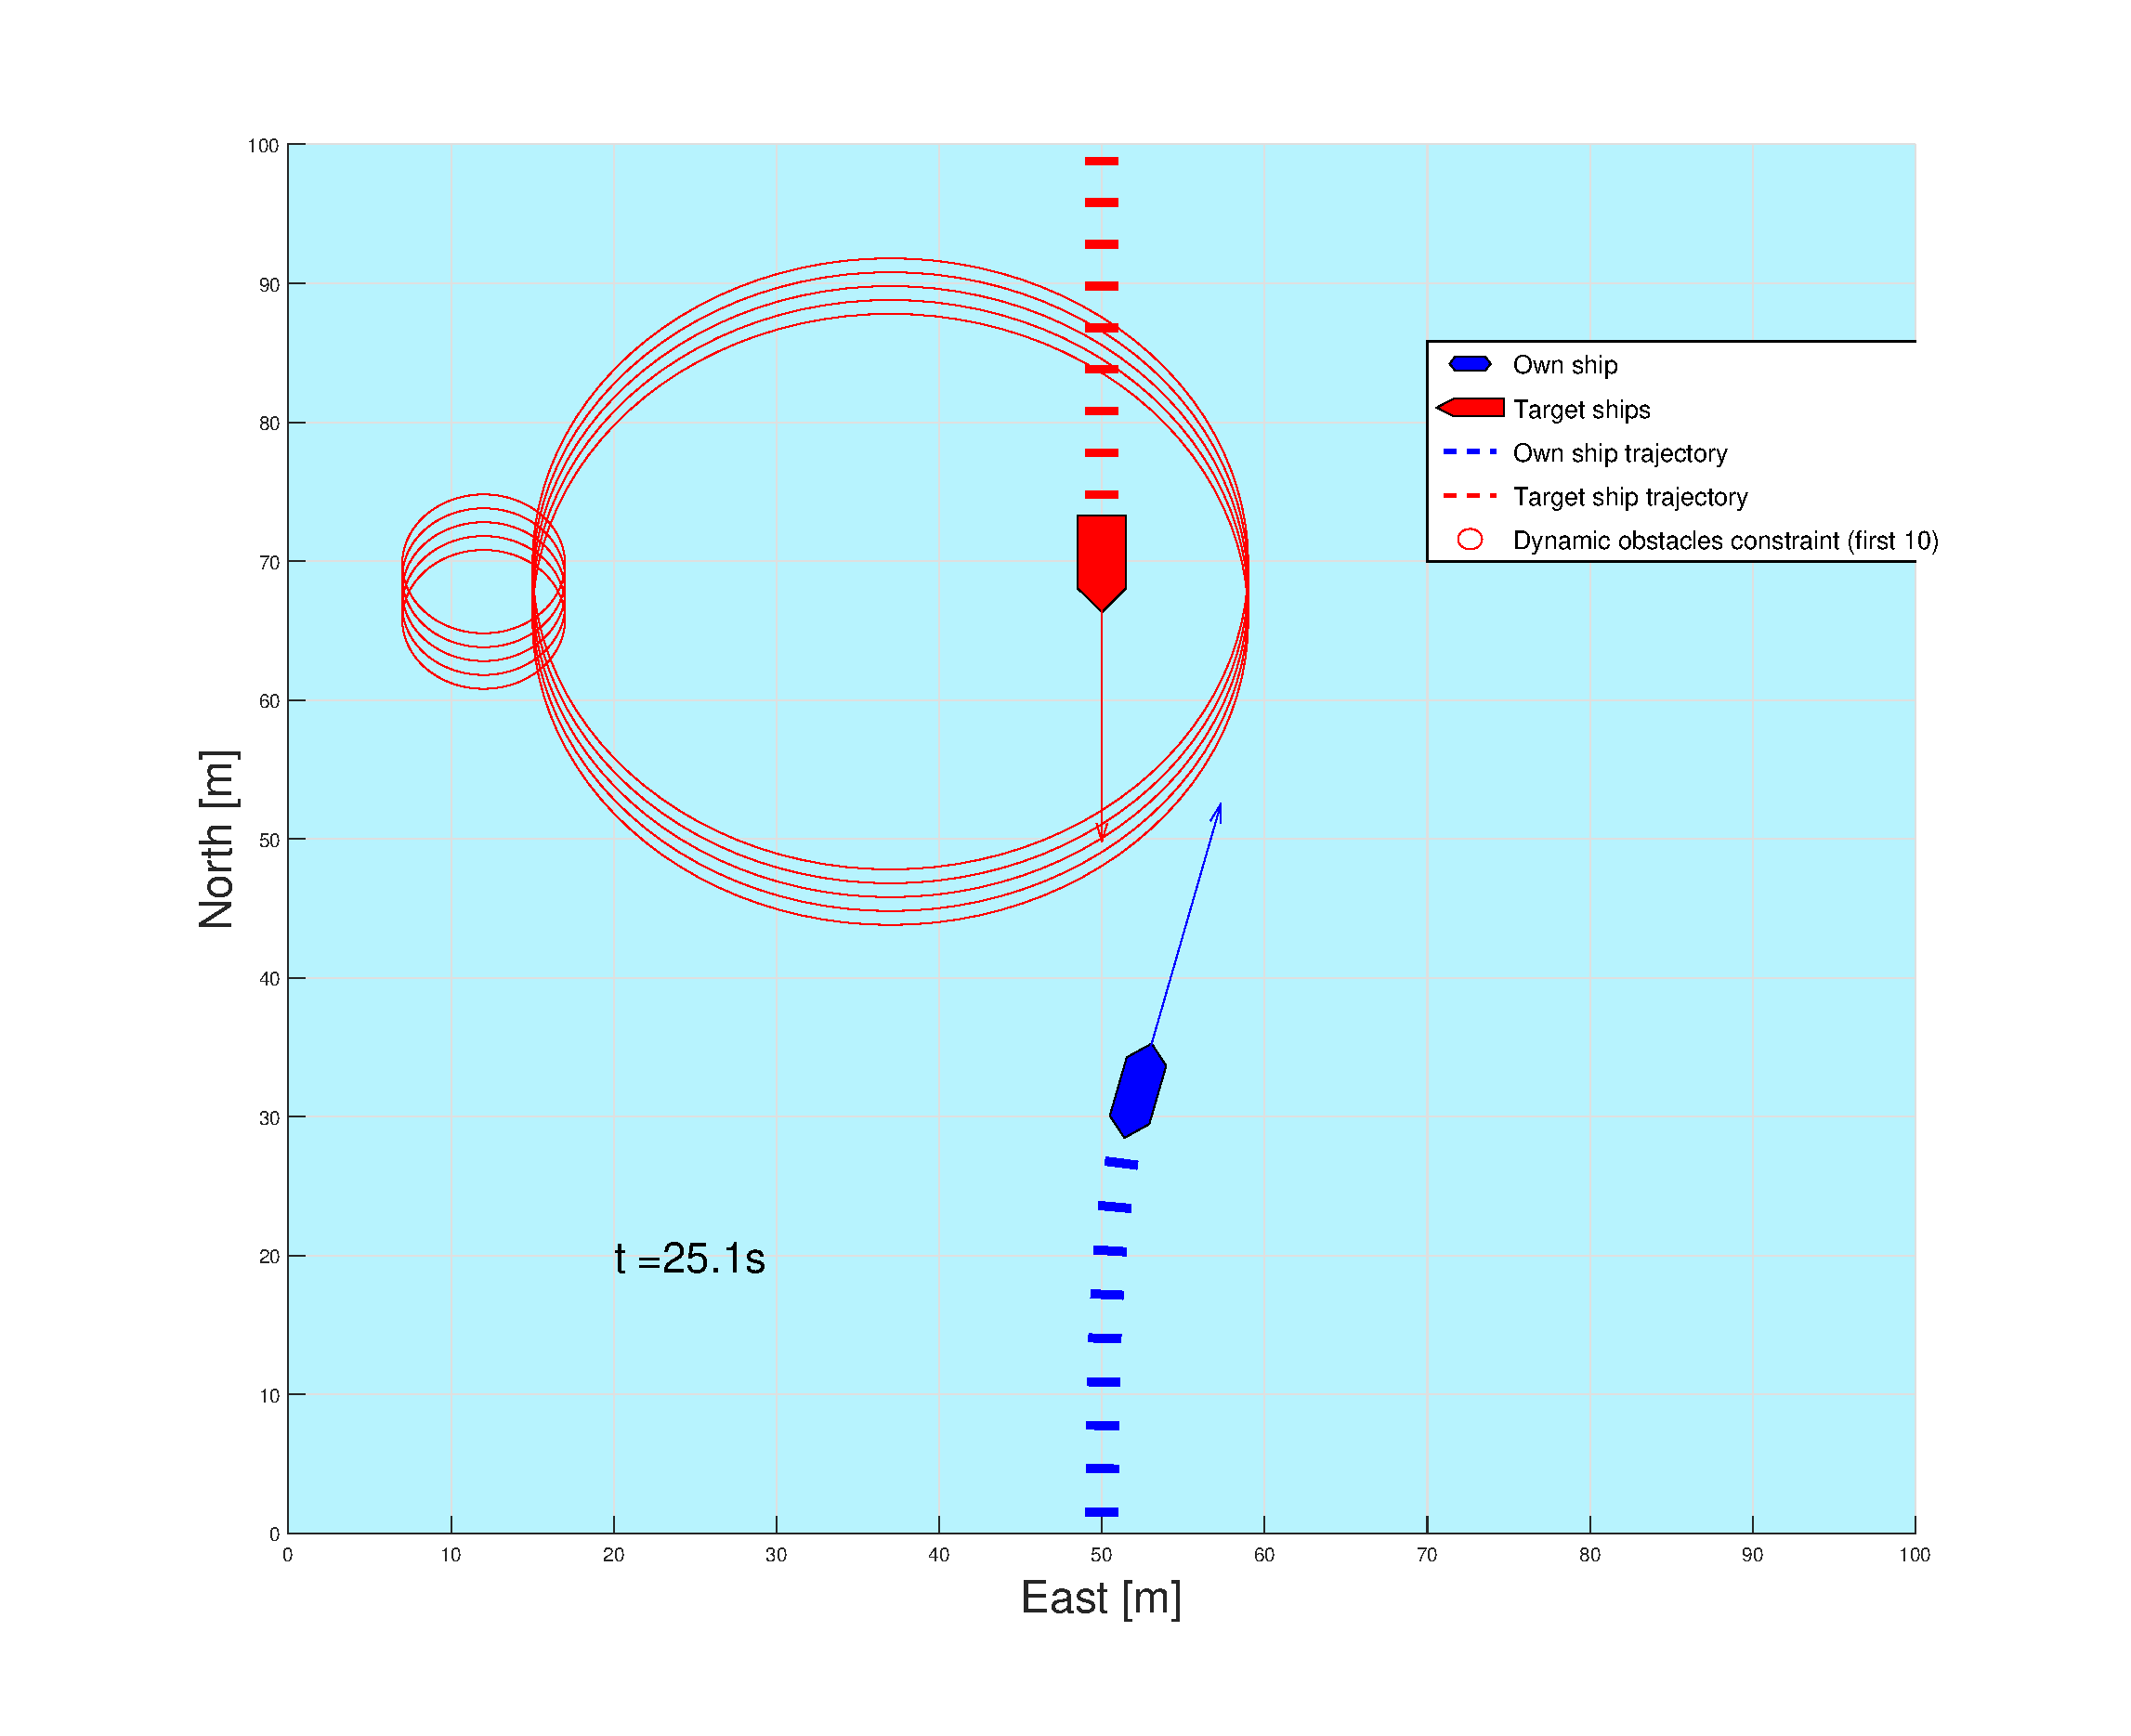
\includegraphics[width=\textwidth]{Images/Figures/enkel_HO/_Simple_1fig1_time=25}
        \subcaption{caption}
    \end{subfigure}
    \hfill
    \begin{subfigure}[b]{0.499\textwidth}
        \centering
        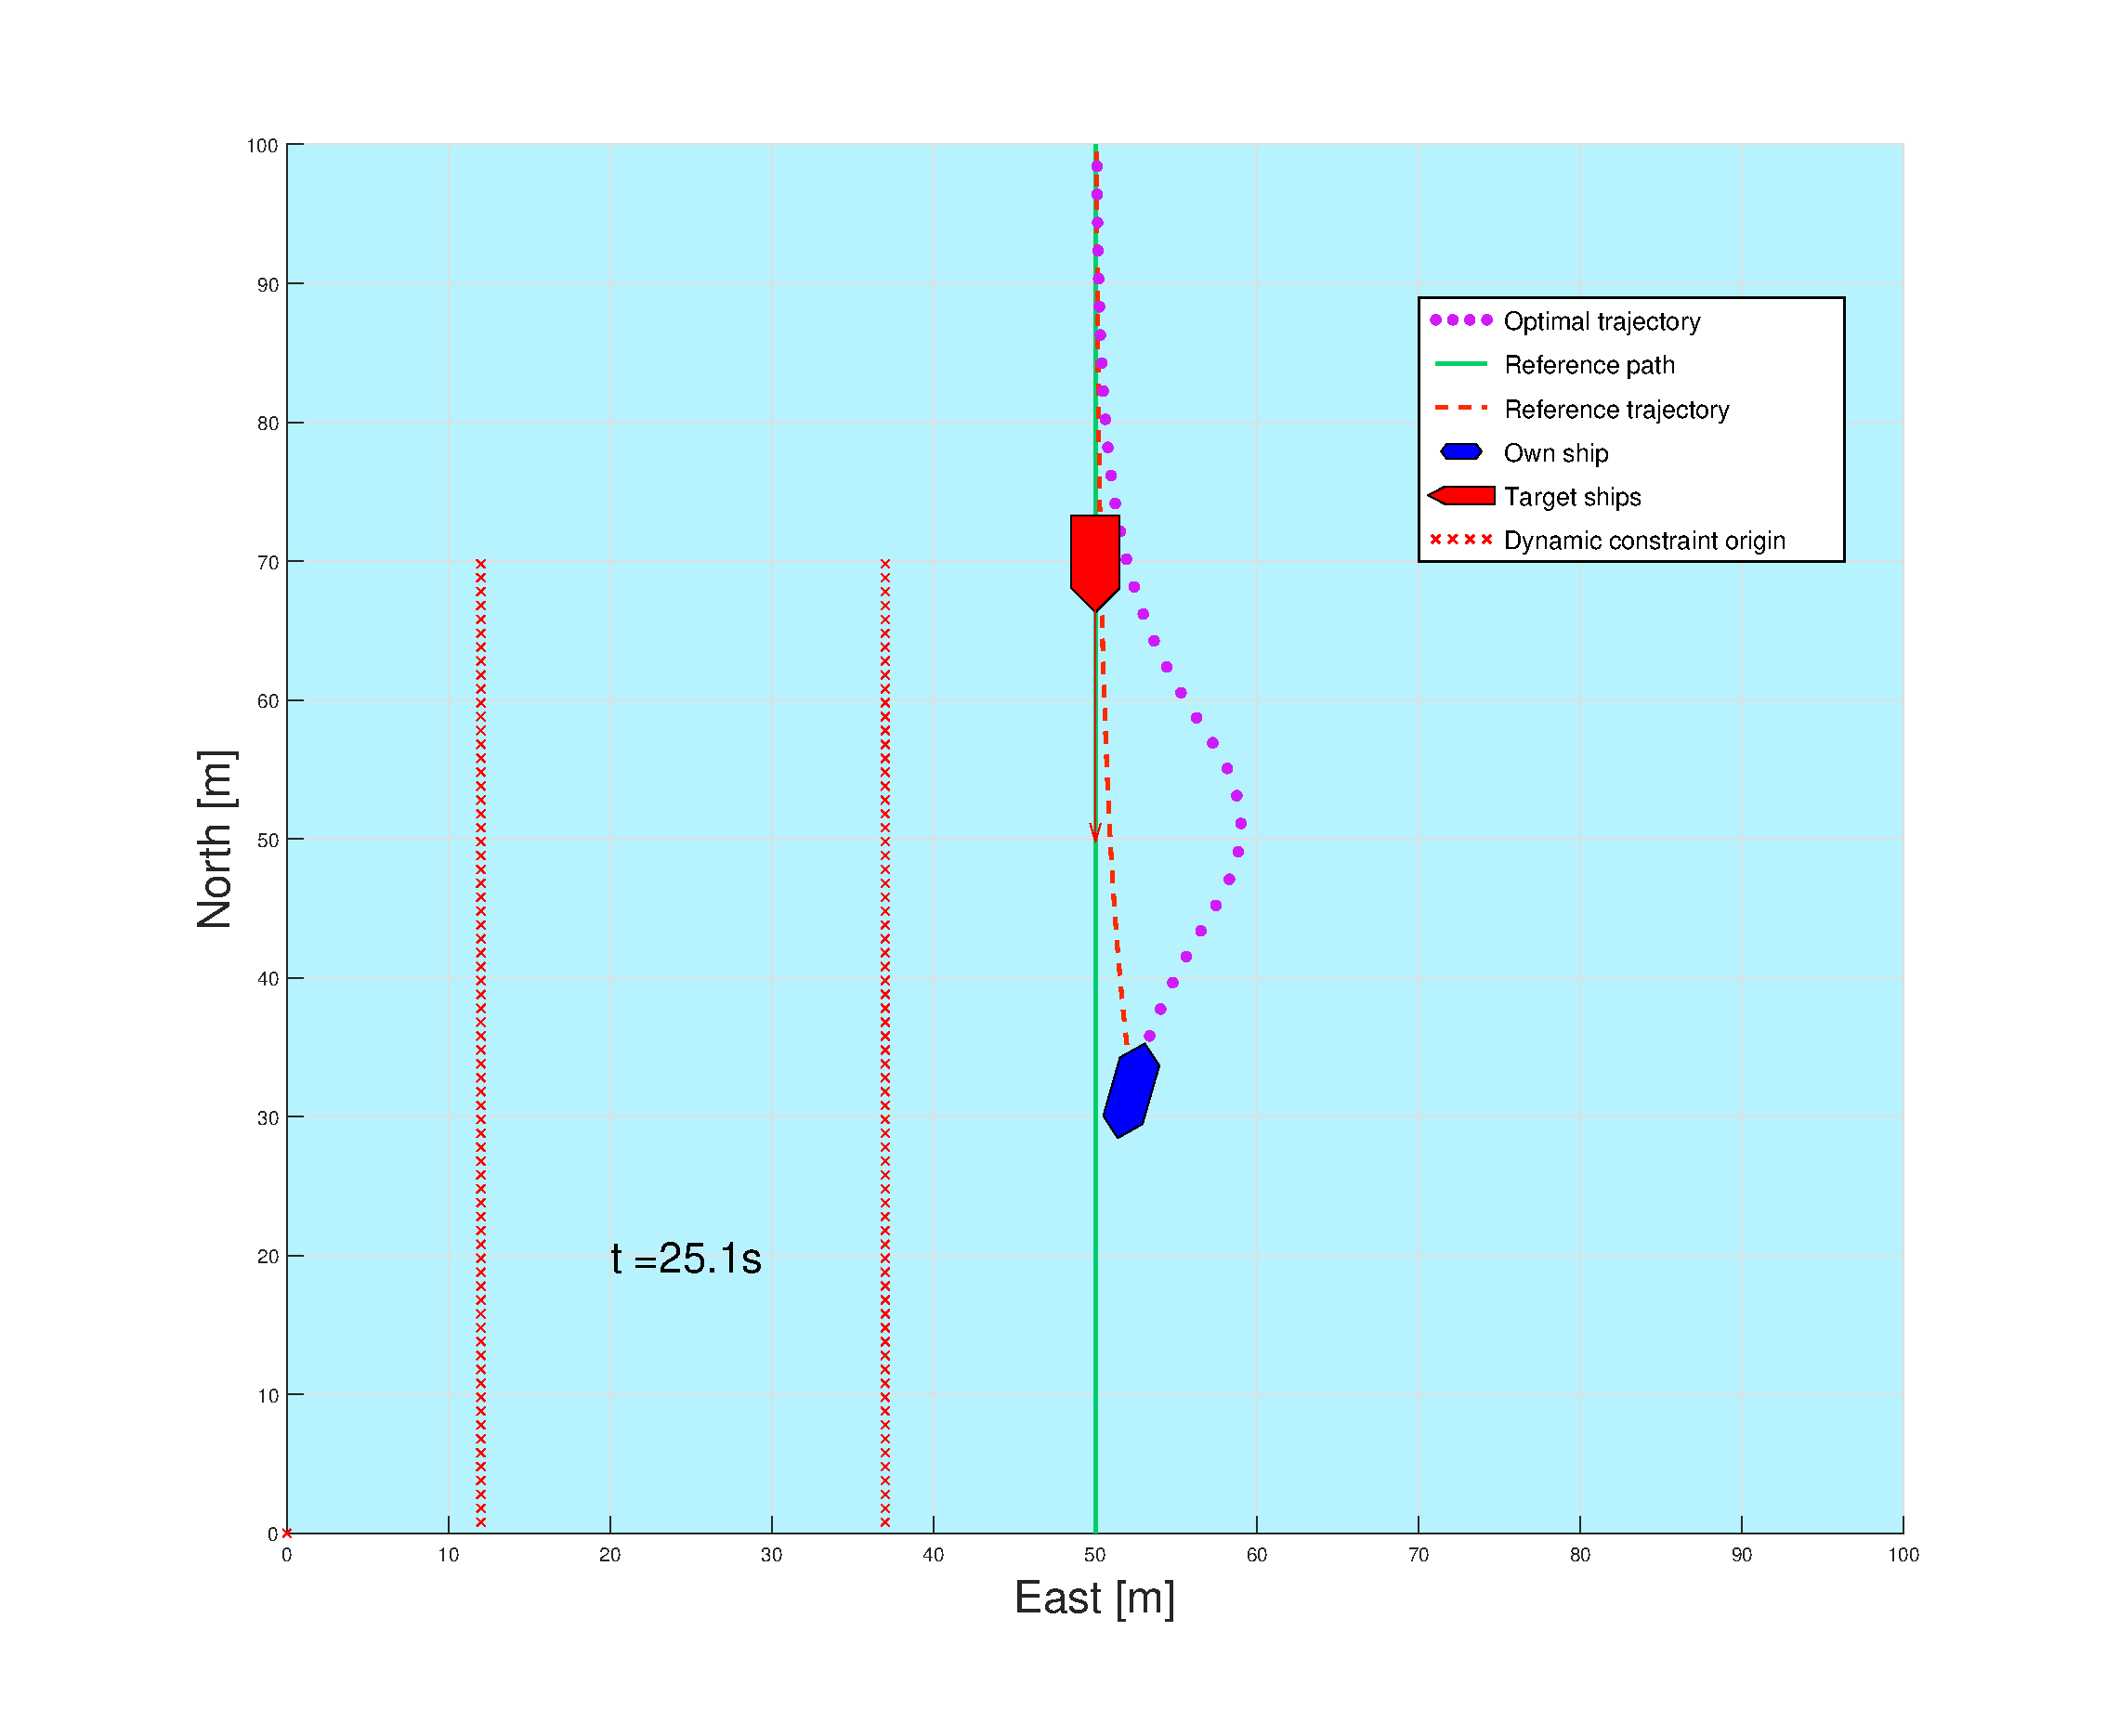
\includegraphics[width=\textwidth]{Images/Figures/enkel_HO/_Simple_1fig999_time=25}
        \subcaption{mhm}
    \end{subfigure}
    \hfill
\end{figure}%
\begin{figure}[ht]\ContinuedFloat
    \begin{subfigure}[b]{0.49\textwidth}
        \centering
        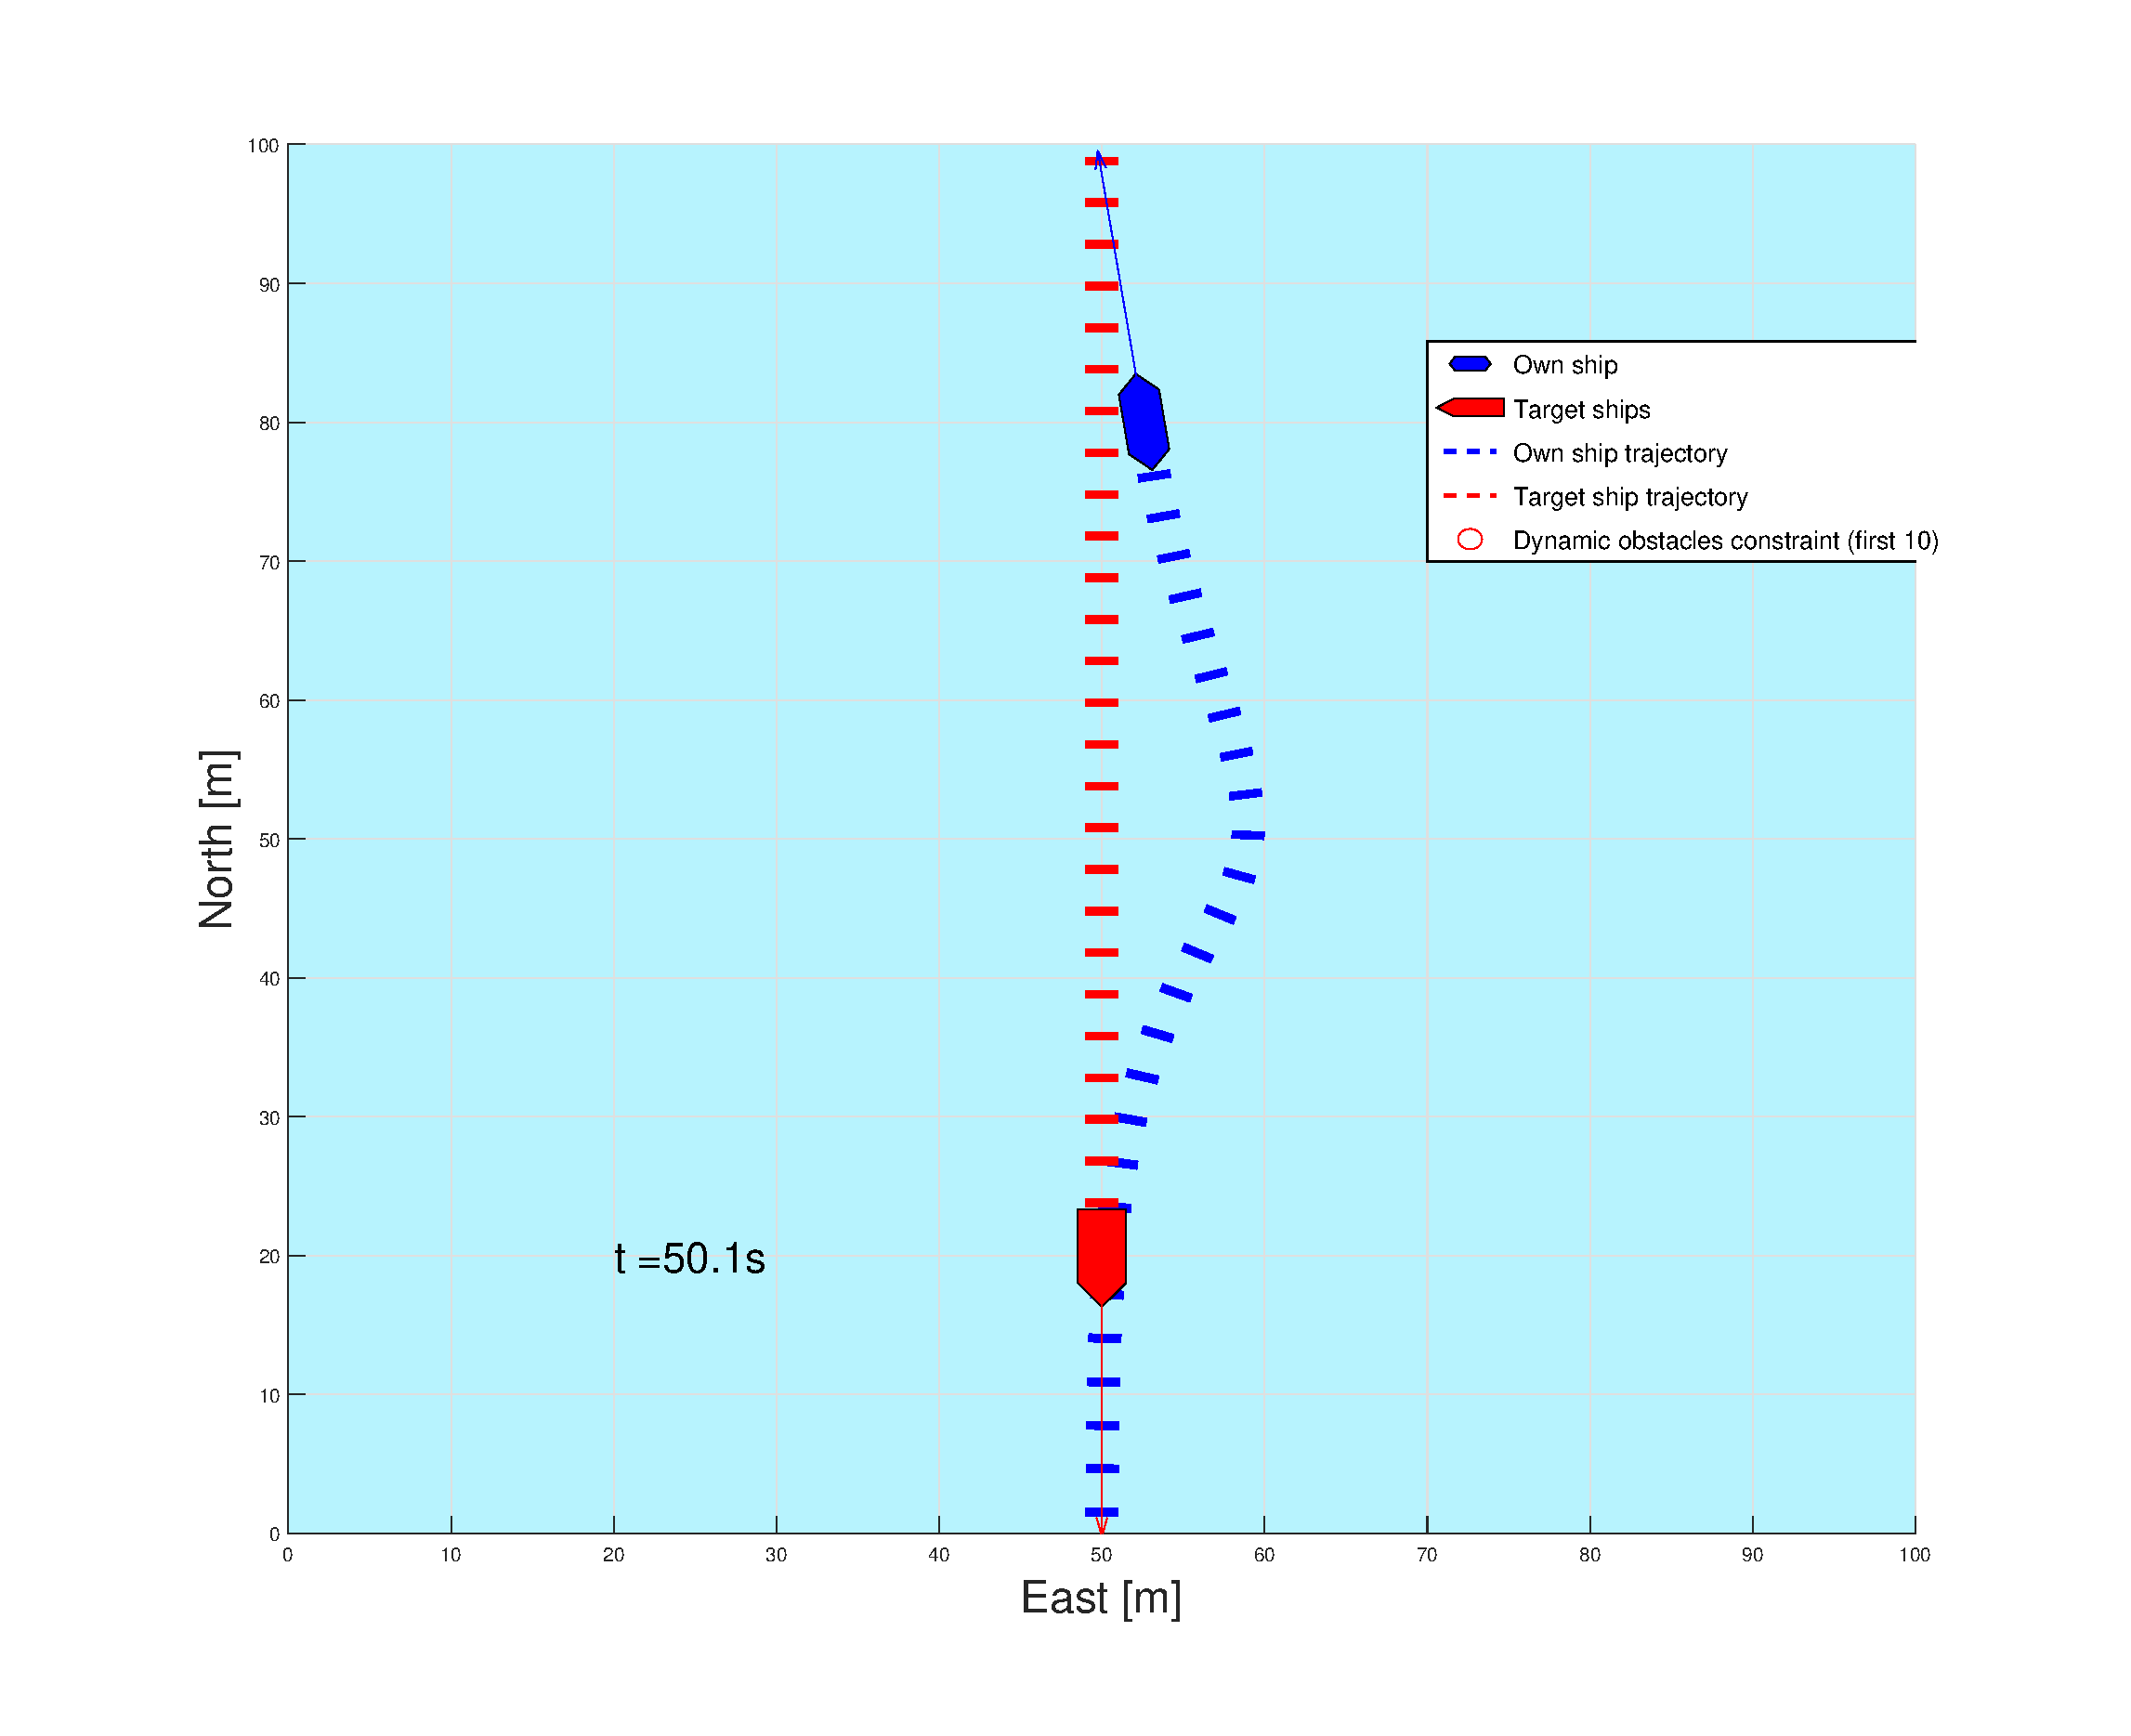
\includegraphics[width=\textwidth]{Images/Figures/enkel_HO/_Simple_1fig1_time=50}
        \subcaption{caption}
    \end{subfigure}
    \hfill
    \begin{subfigure}[b]{0.499\textwidth}
        \centering
        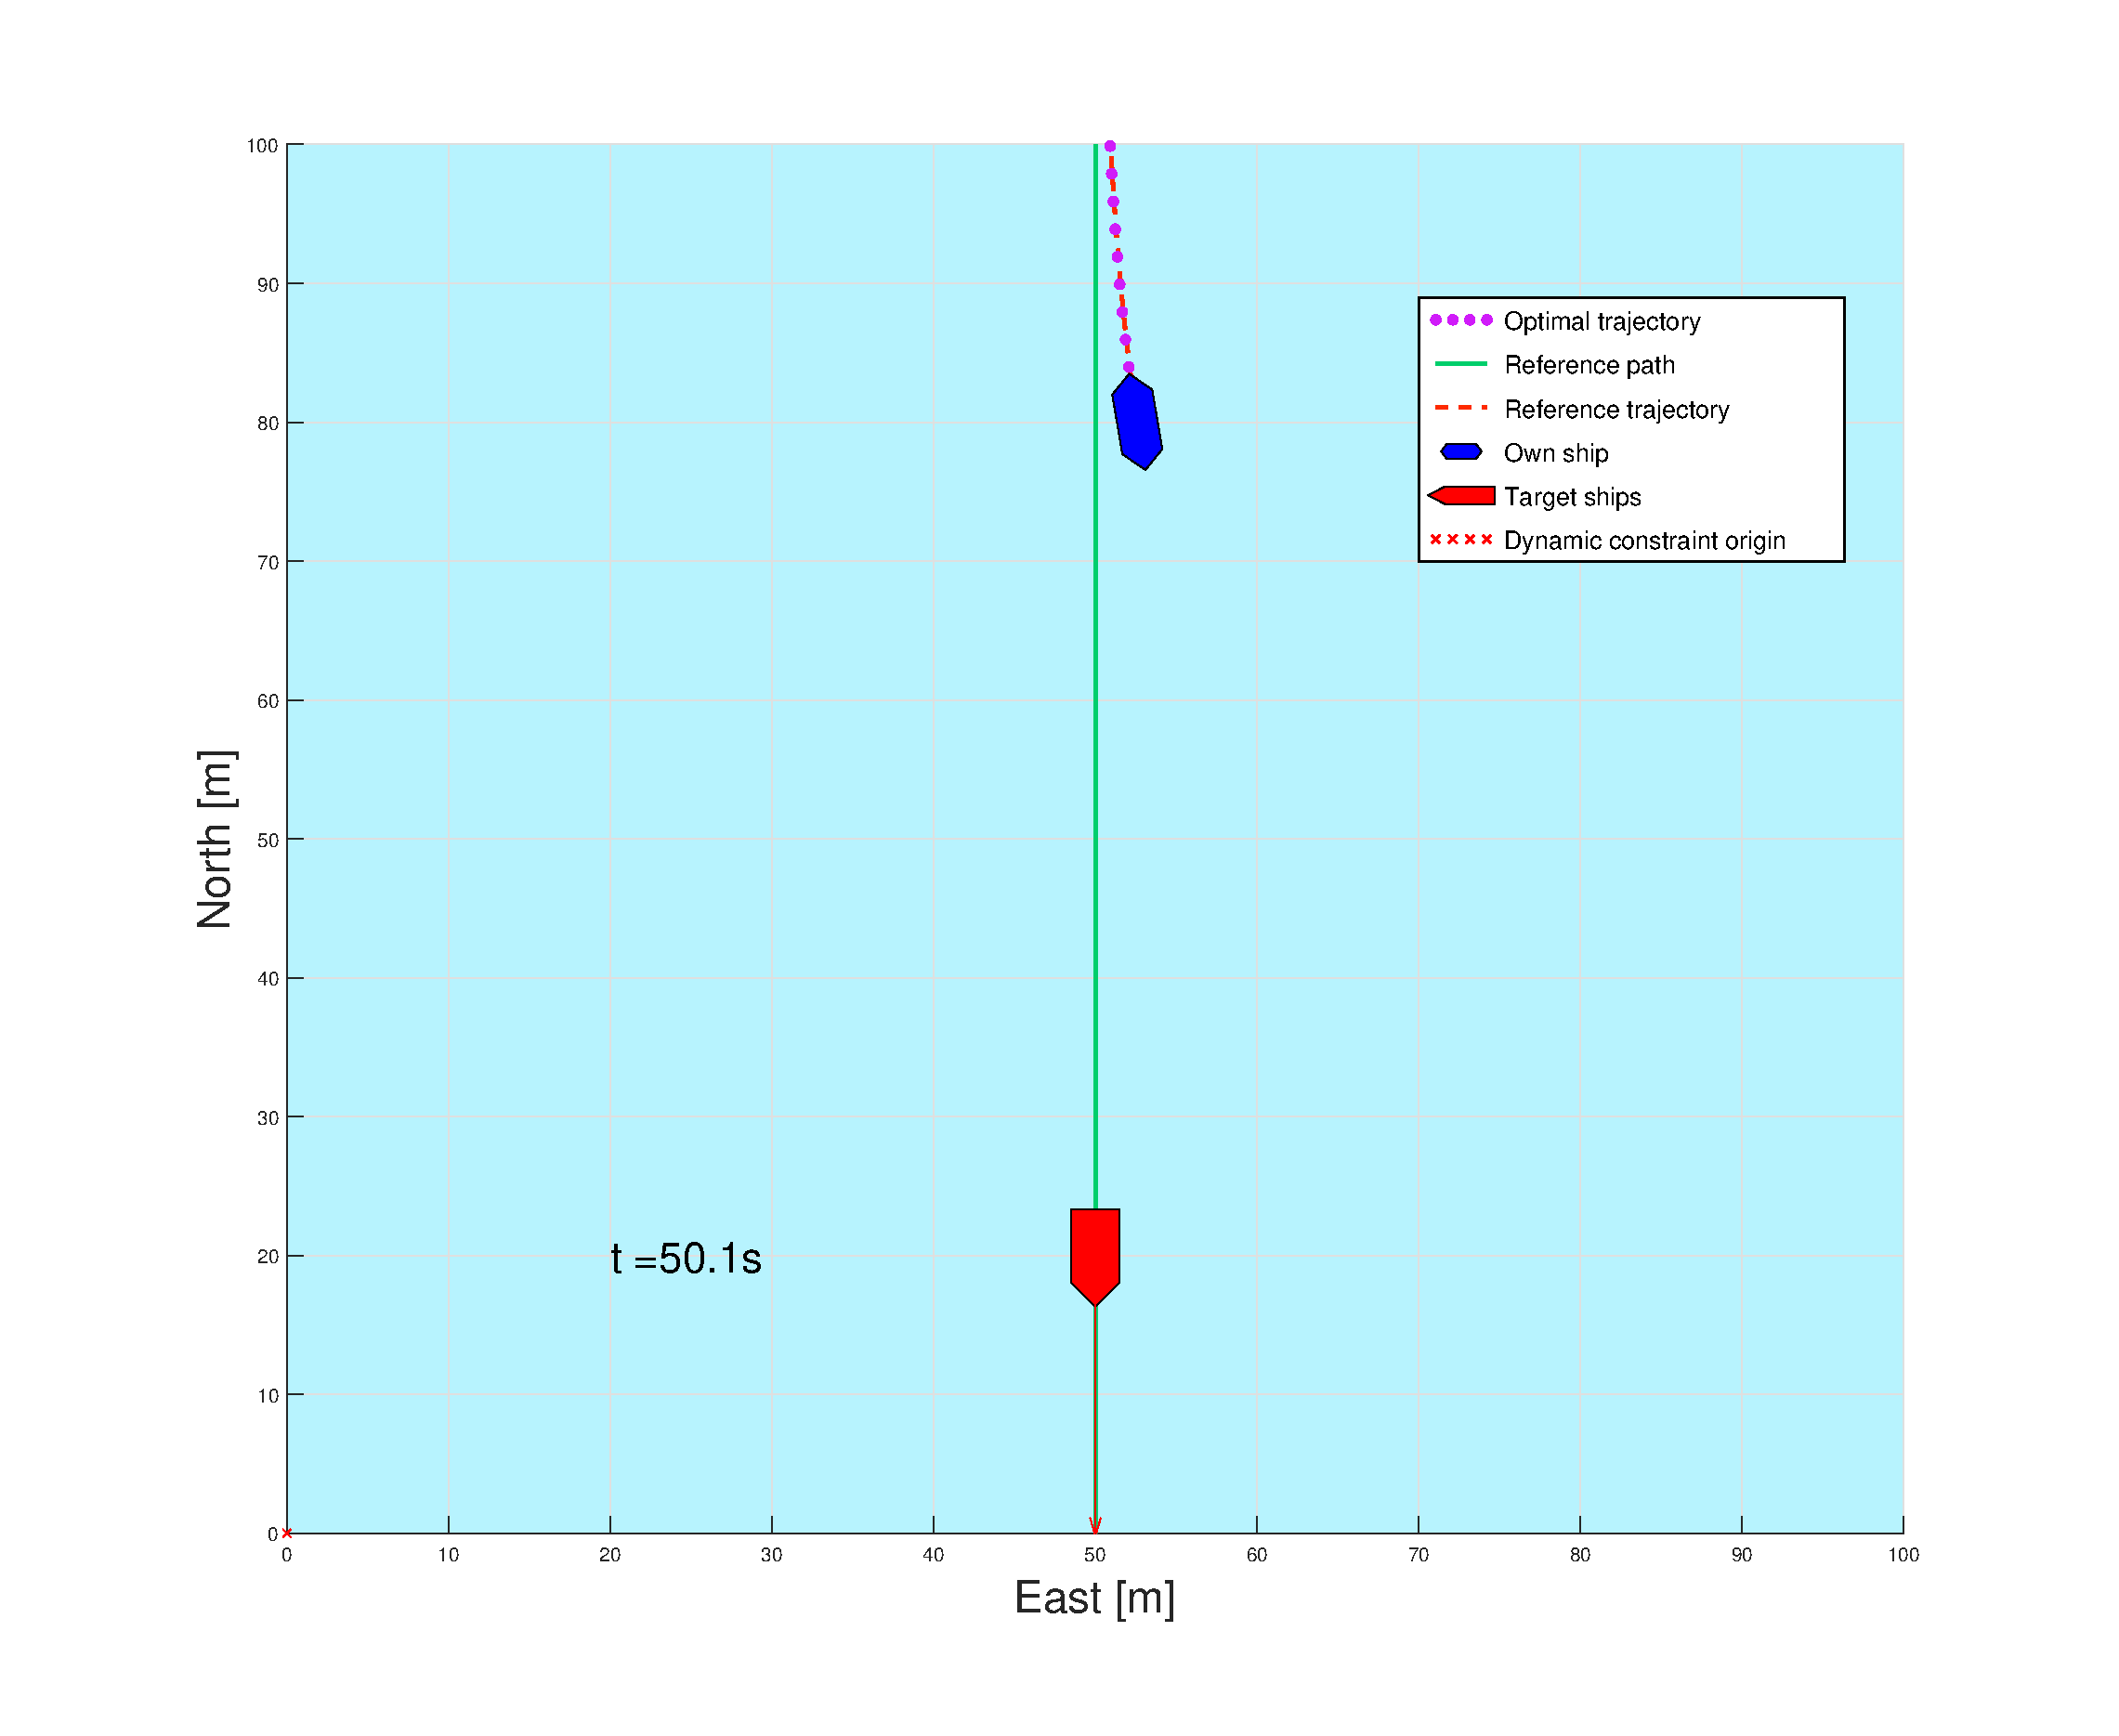
\includegraphics[width=\textwidth]{Images/Figures/enkel_HO/_Simple_1fig999_time=50}
        \subcaption{mhm}
    \end{subfigure}
    \hfill
    \\
    \begin{subfigure}[b]{0.49\textwidth}
        \centering
        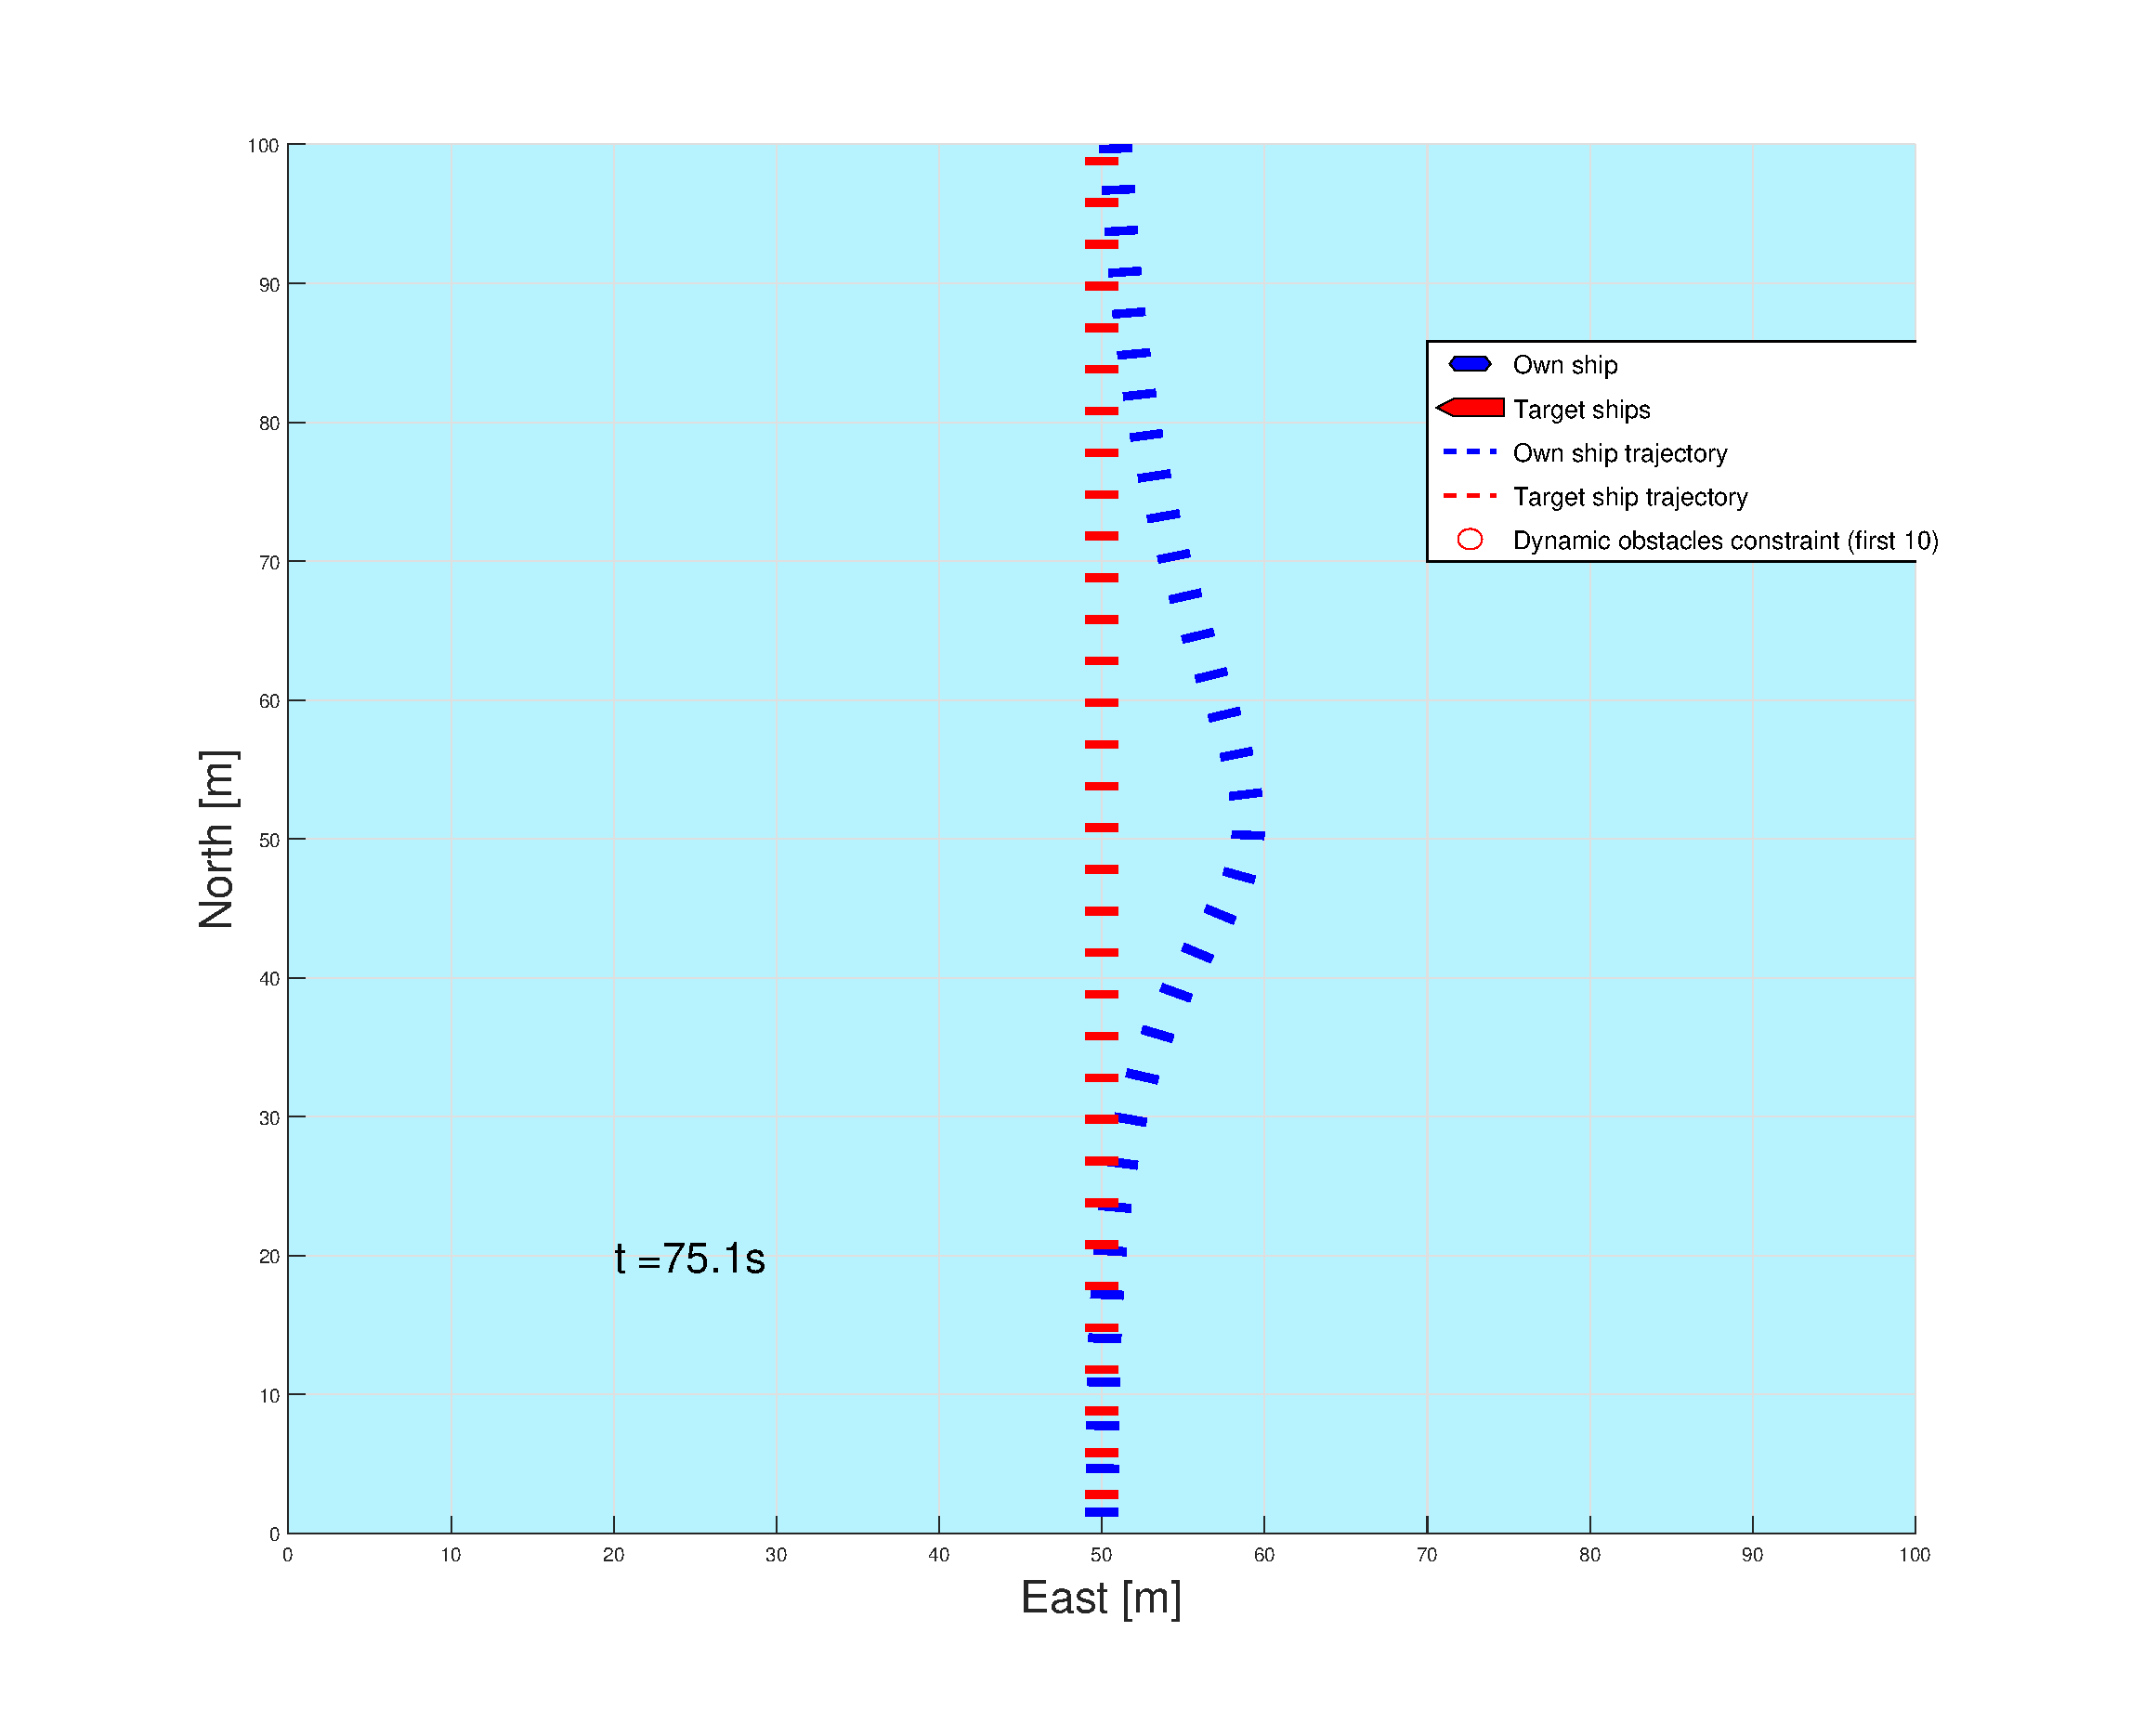
\includegraphics[width=\textwidth]{Images/Figures/enkel_HO/_Simple_1fig1_time=75}
        \subcaption{caption}
    \end{subfigure}
    \hfill
    \begin{subfigure}[b]{0.499\textwidth}
        \centering
        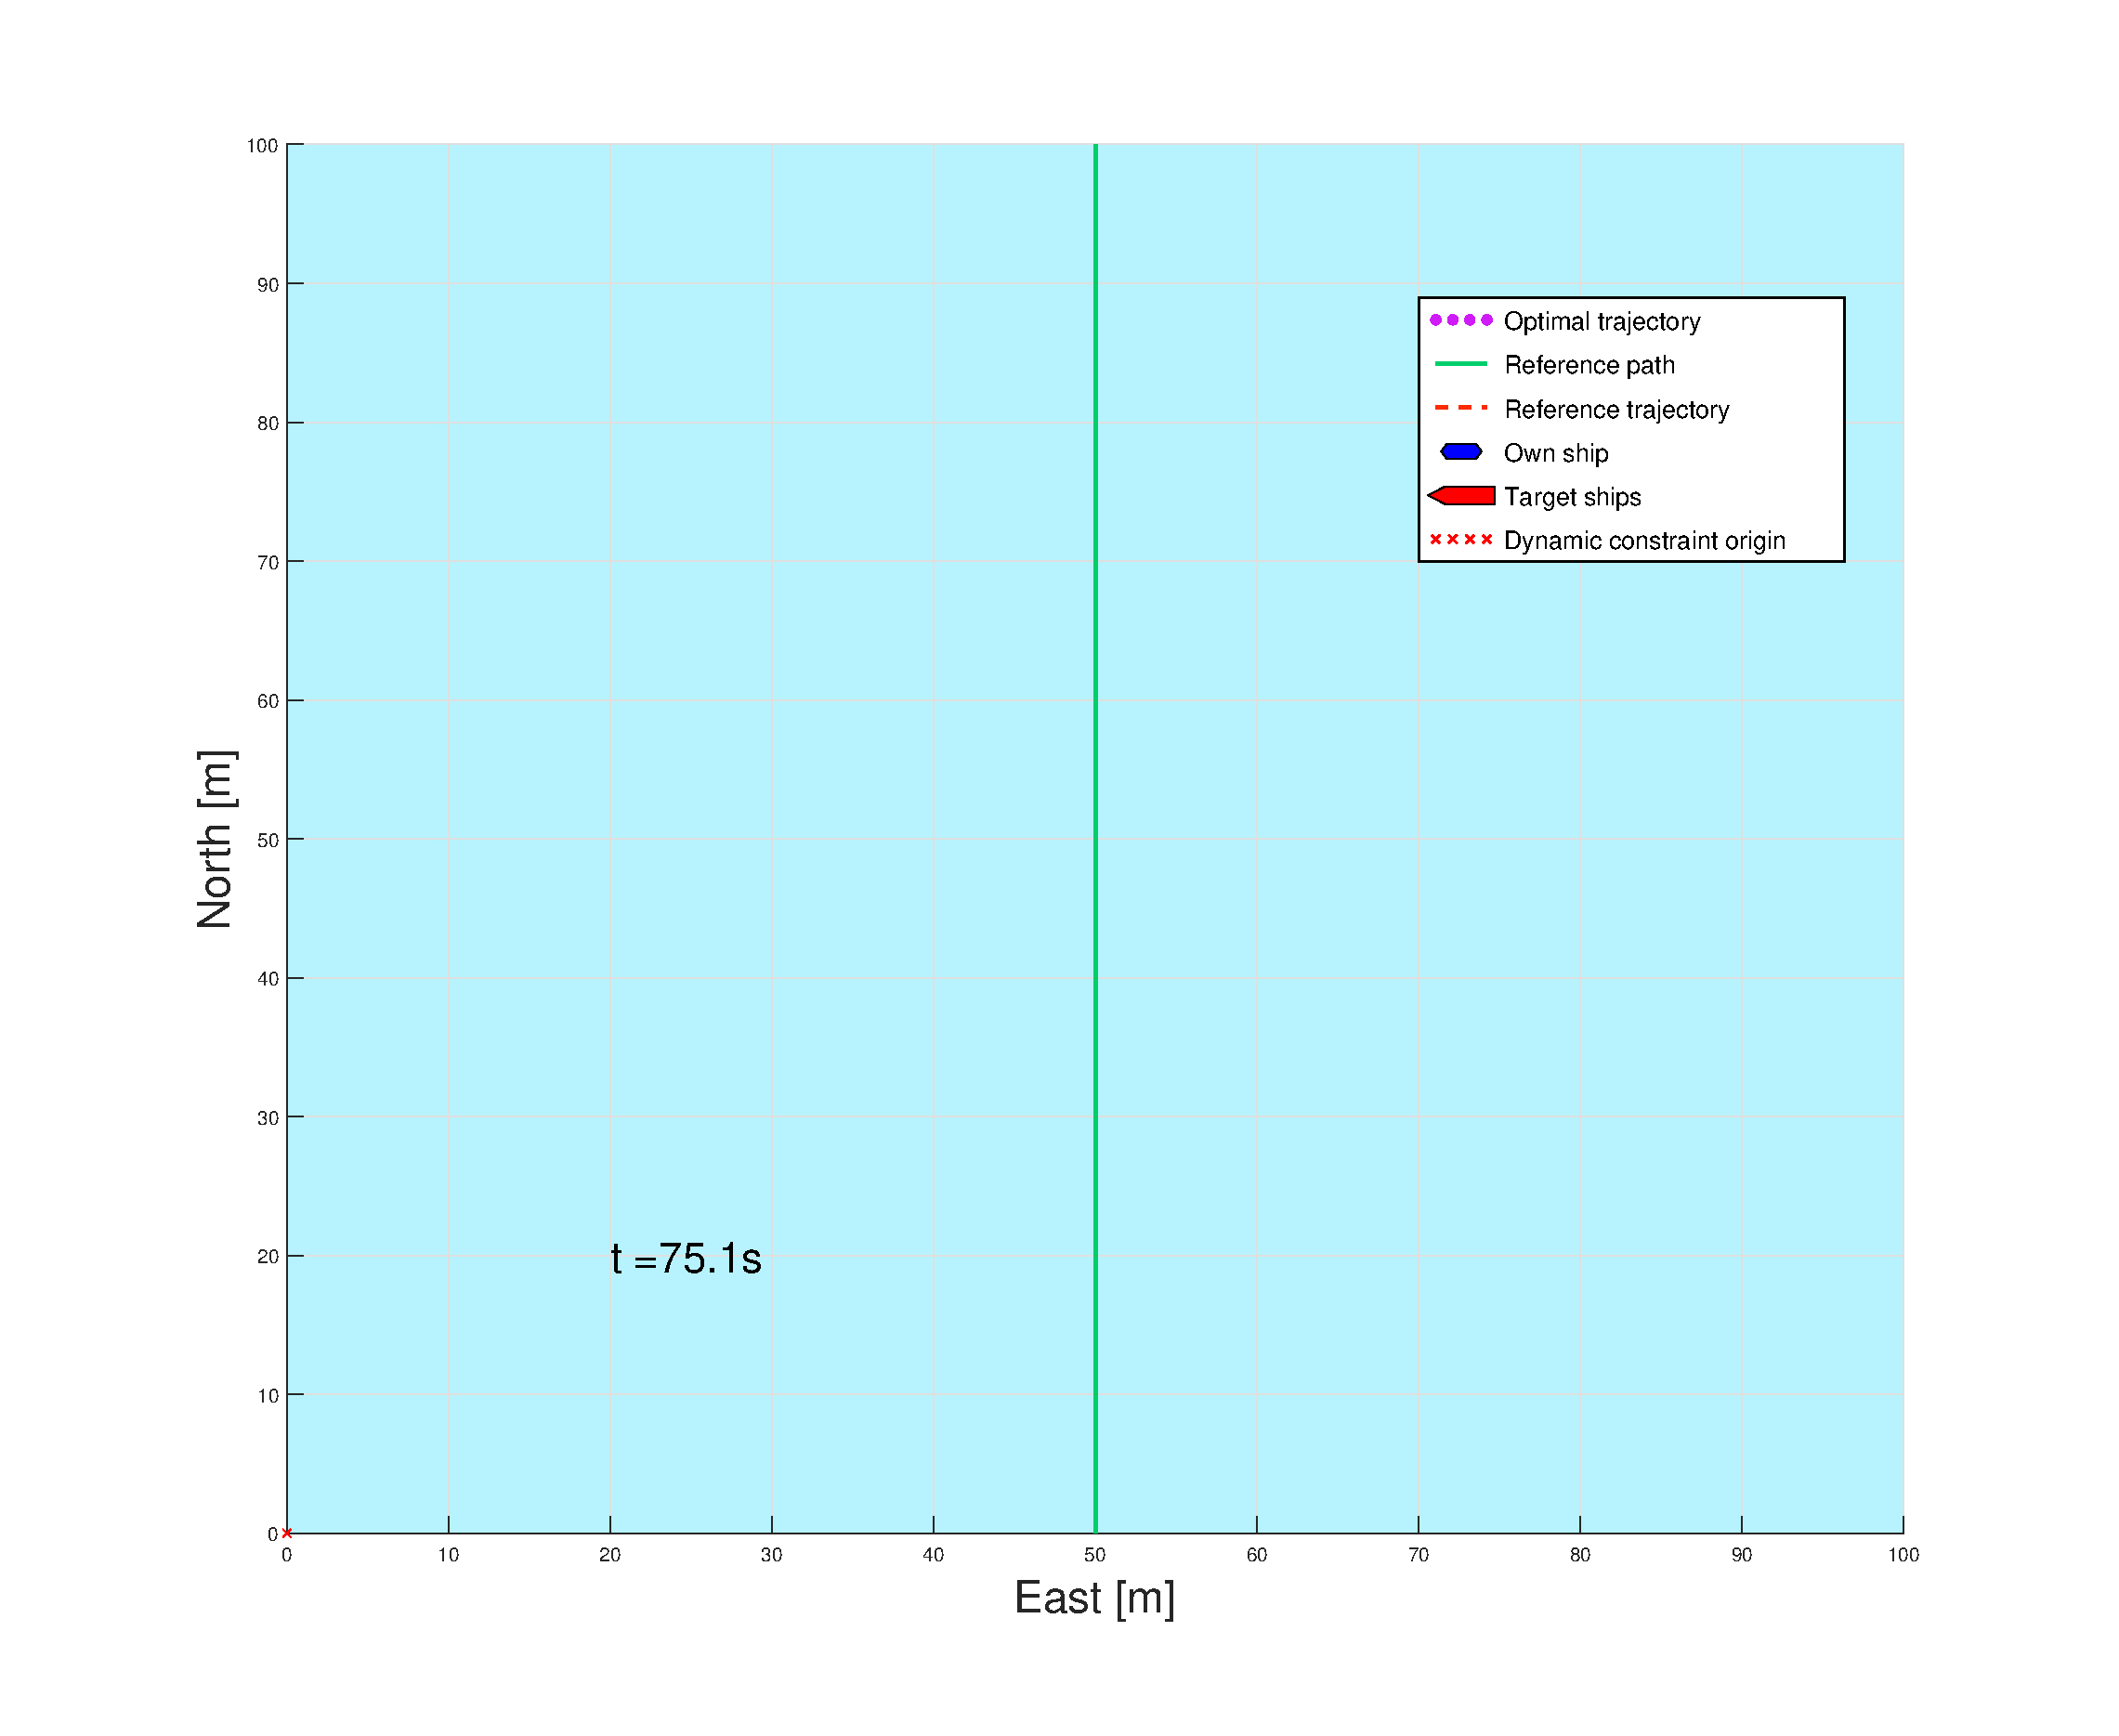
\includegraphics[width=\textwidth]{Images/Figures/enkel_HO/_Simple_1fig999_time=75}
        \subcaption{mhm}
    \end{subfigure}
    \hfill
    \caption{Simple Head on Without Prediction}
\end{figure}

\subsubsection{Simple Give Way}
\begin{itemize}
    \item It would be highly unusual to start using the trajectory planner when alredy this close to a situation
    \item This is reflected in the strange behaviour where our path is completely blocked when dynamic obstacle constrains are enabled.
    \item otherwise the behaviour ends up being exactly as expected considering the placements of the constraints.
\end{itemize}
\clearpage
\begin{figure}[!b]
    \begin{subfigure}[b]{0.49\textwidth}
        \centering
        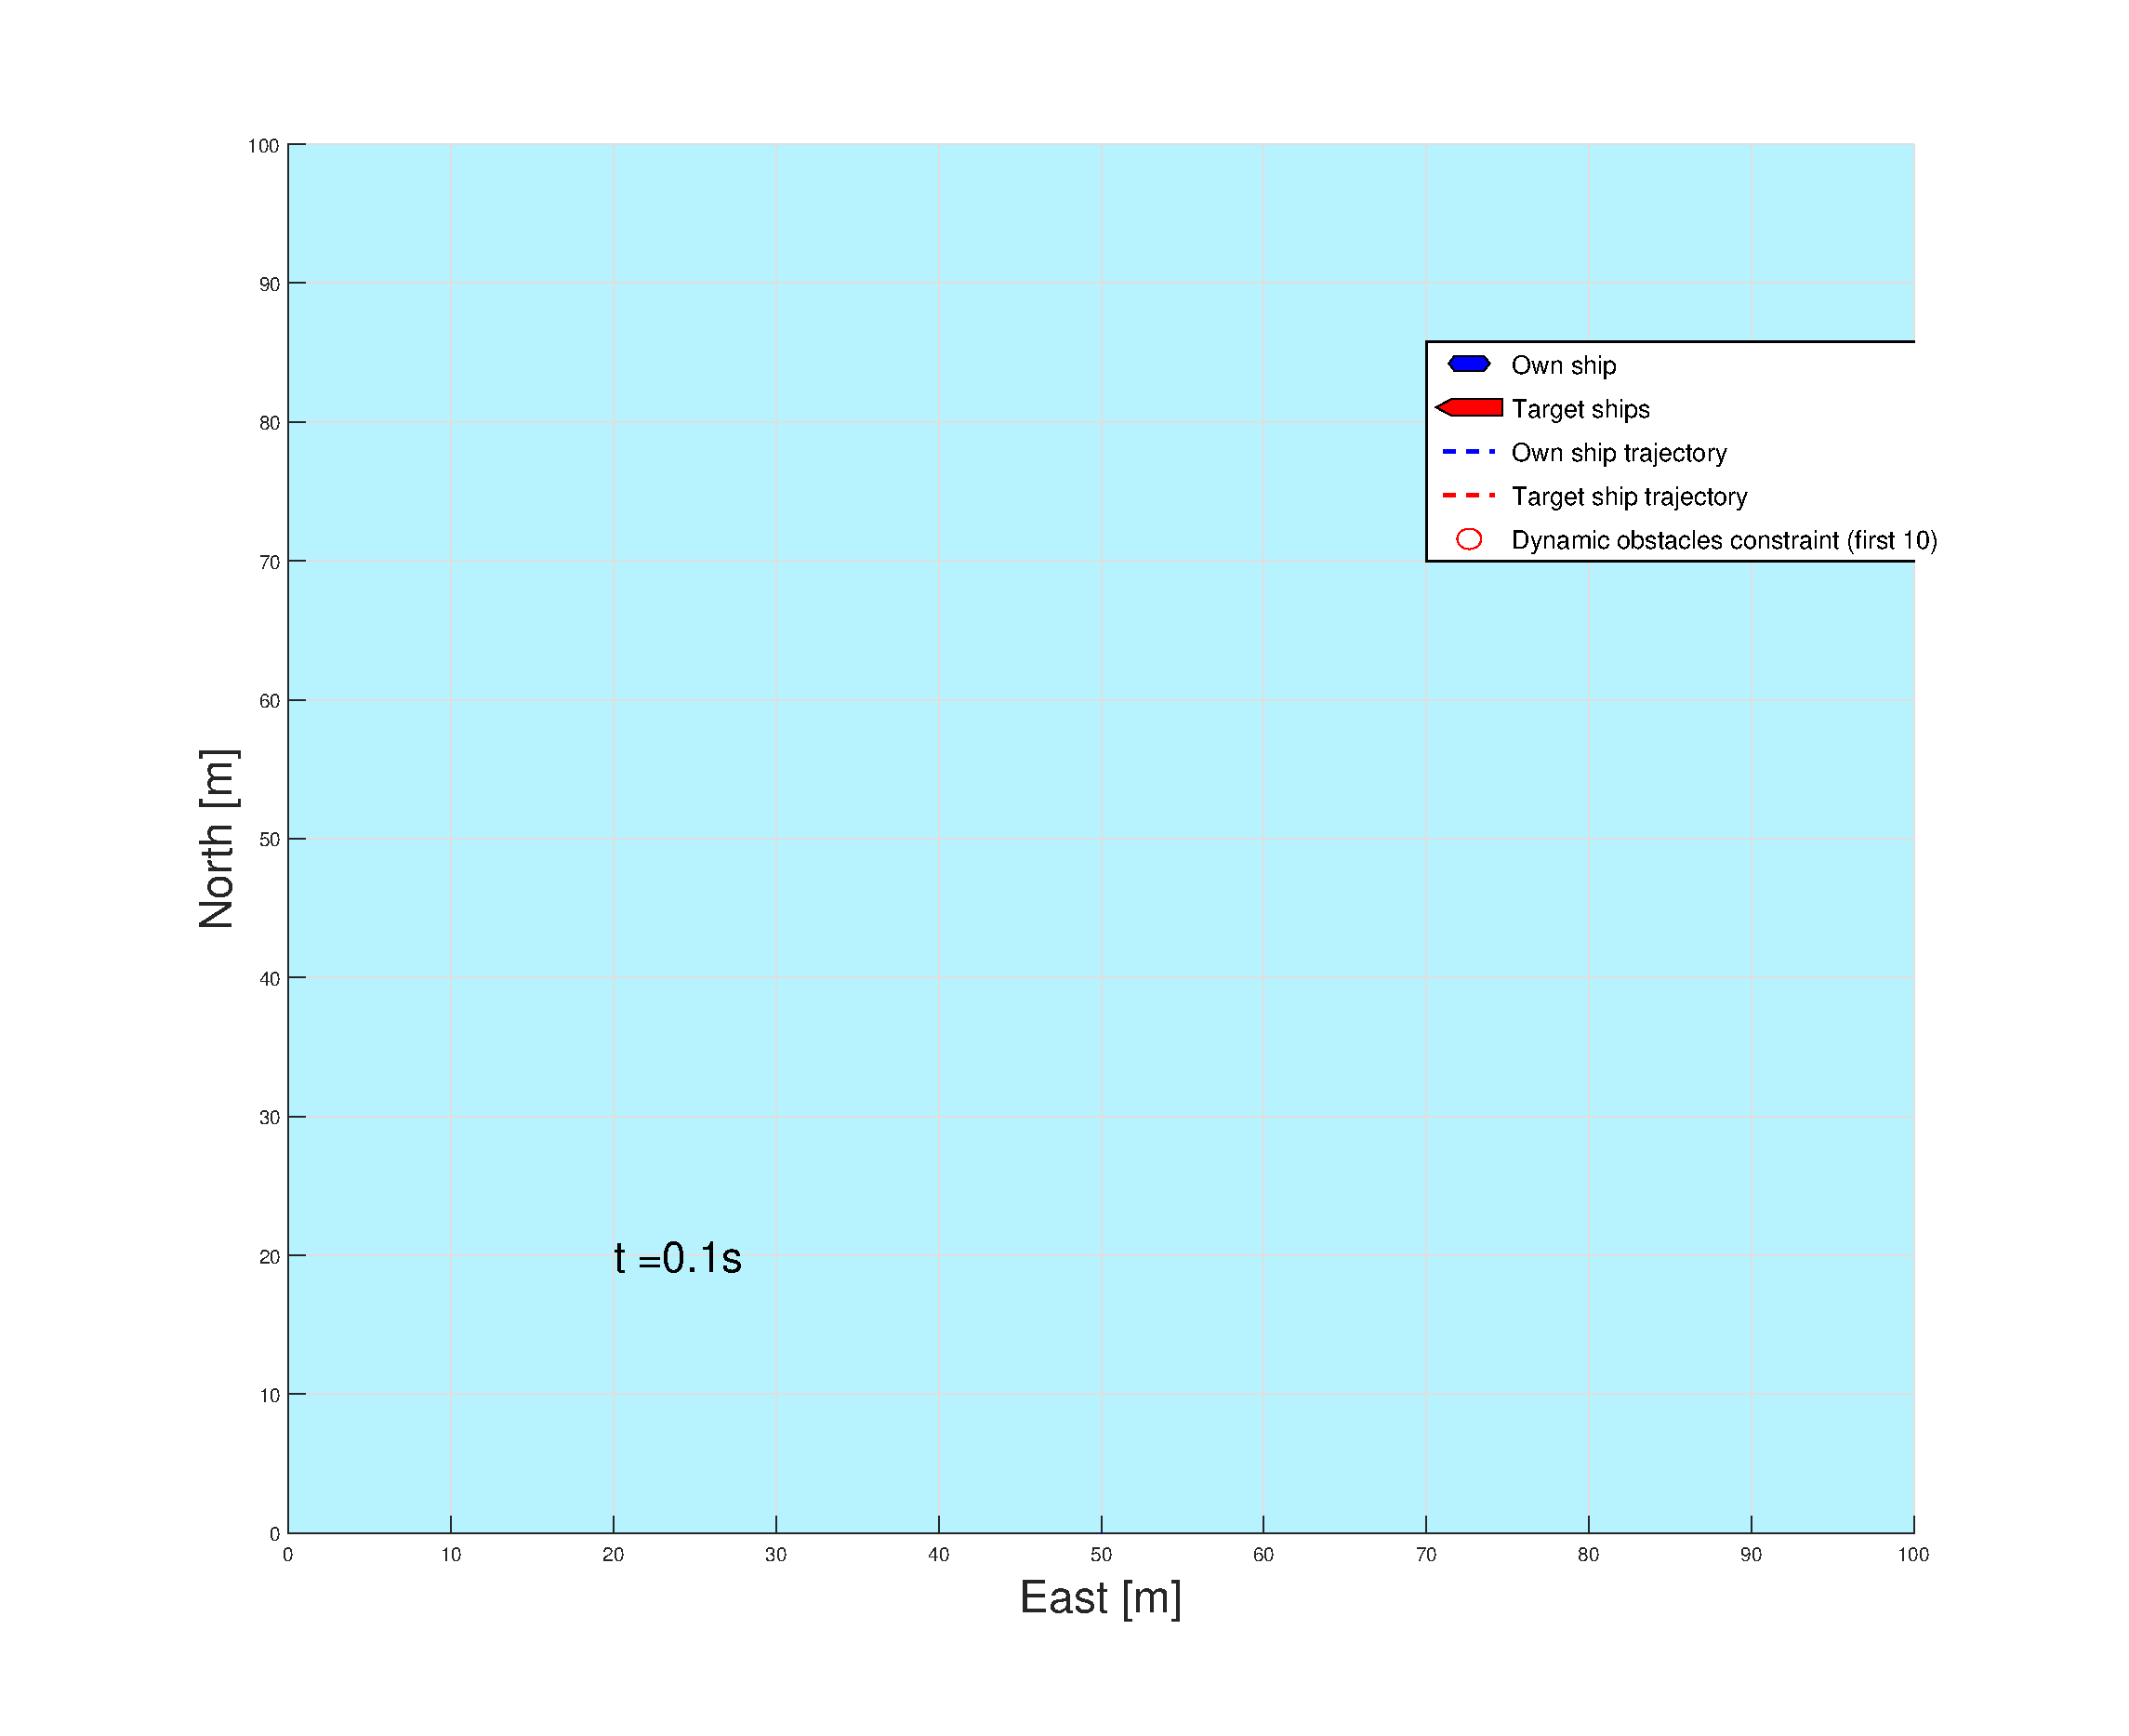
\includegraphics[width=\textwidth]{Images/Figures/enkel_GW/_Simple_0fig1_time=0}
        \subcaption{caption}
    \end{subfigure}
    \hfill
    \begin{subfigure}[b]{0.499\textwidth}
        \centering
        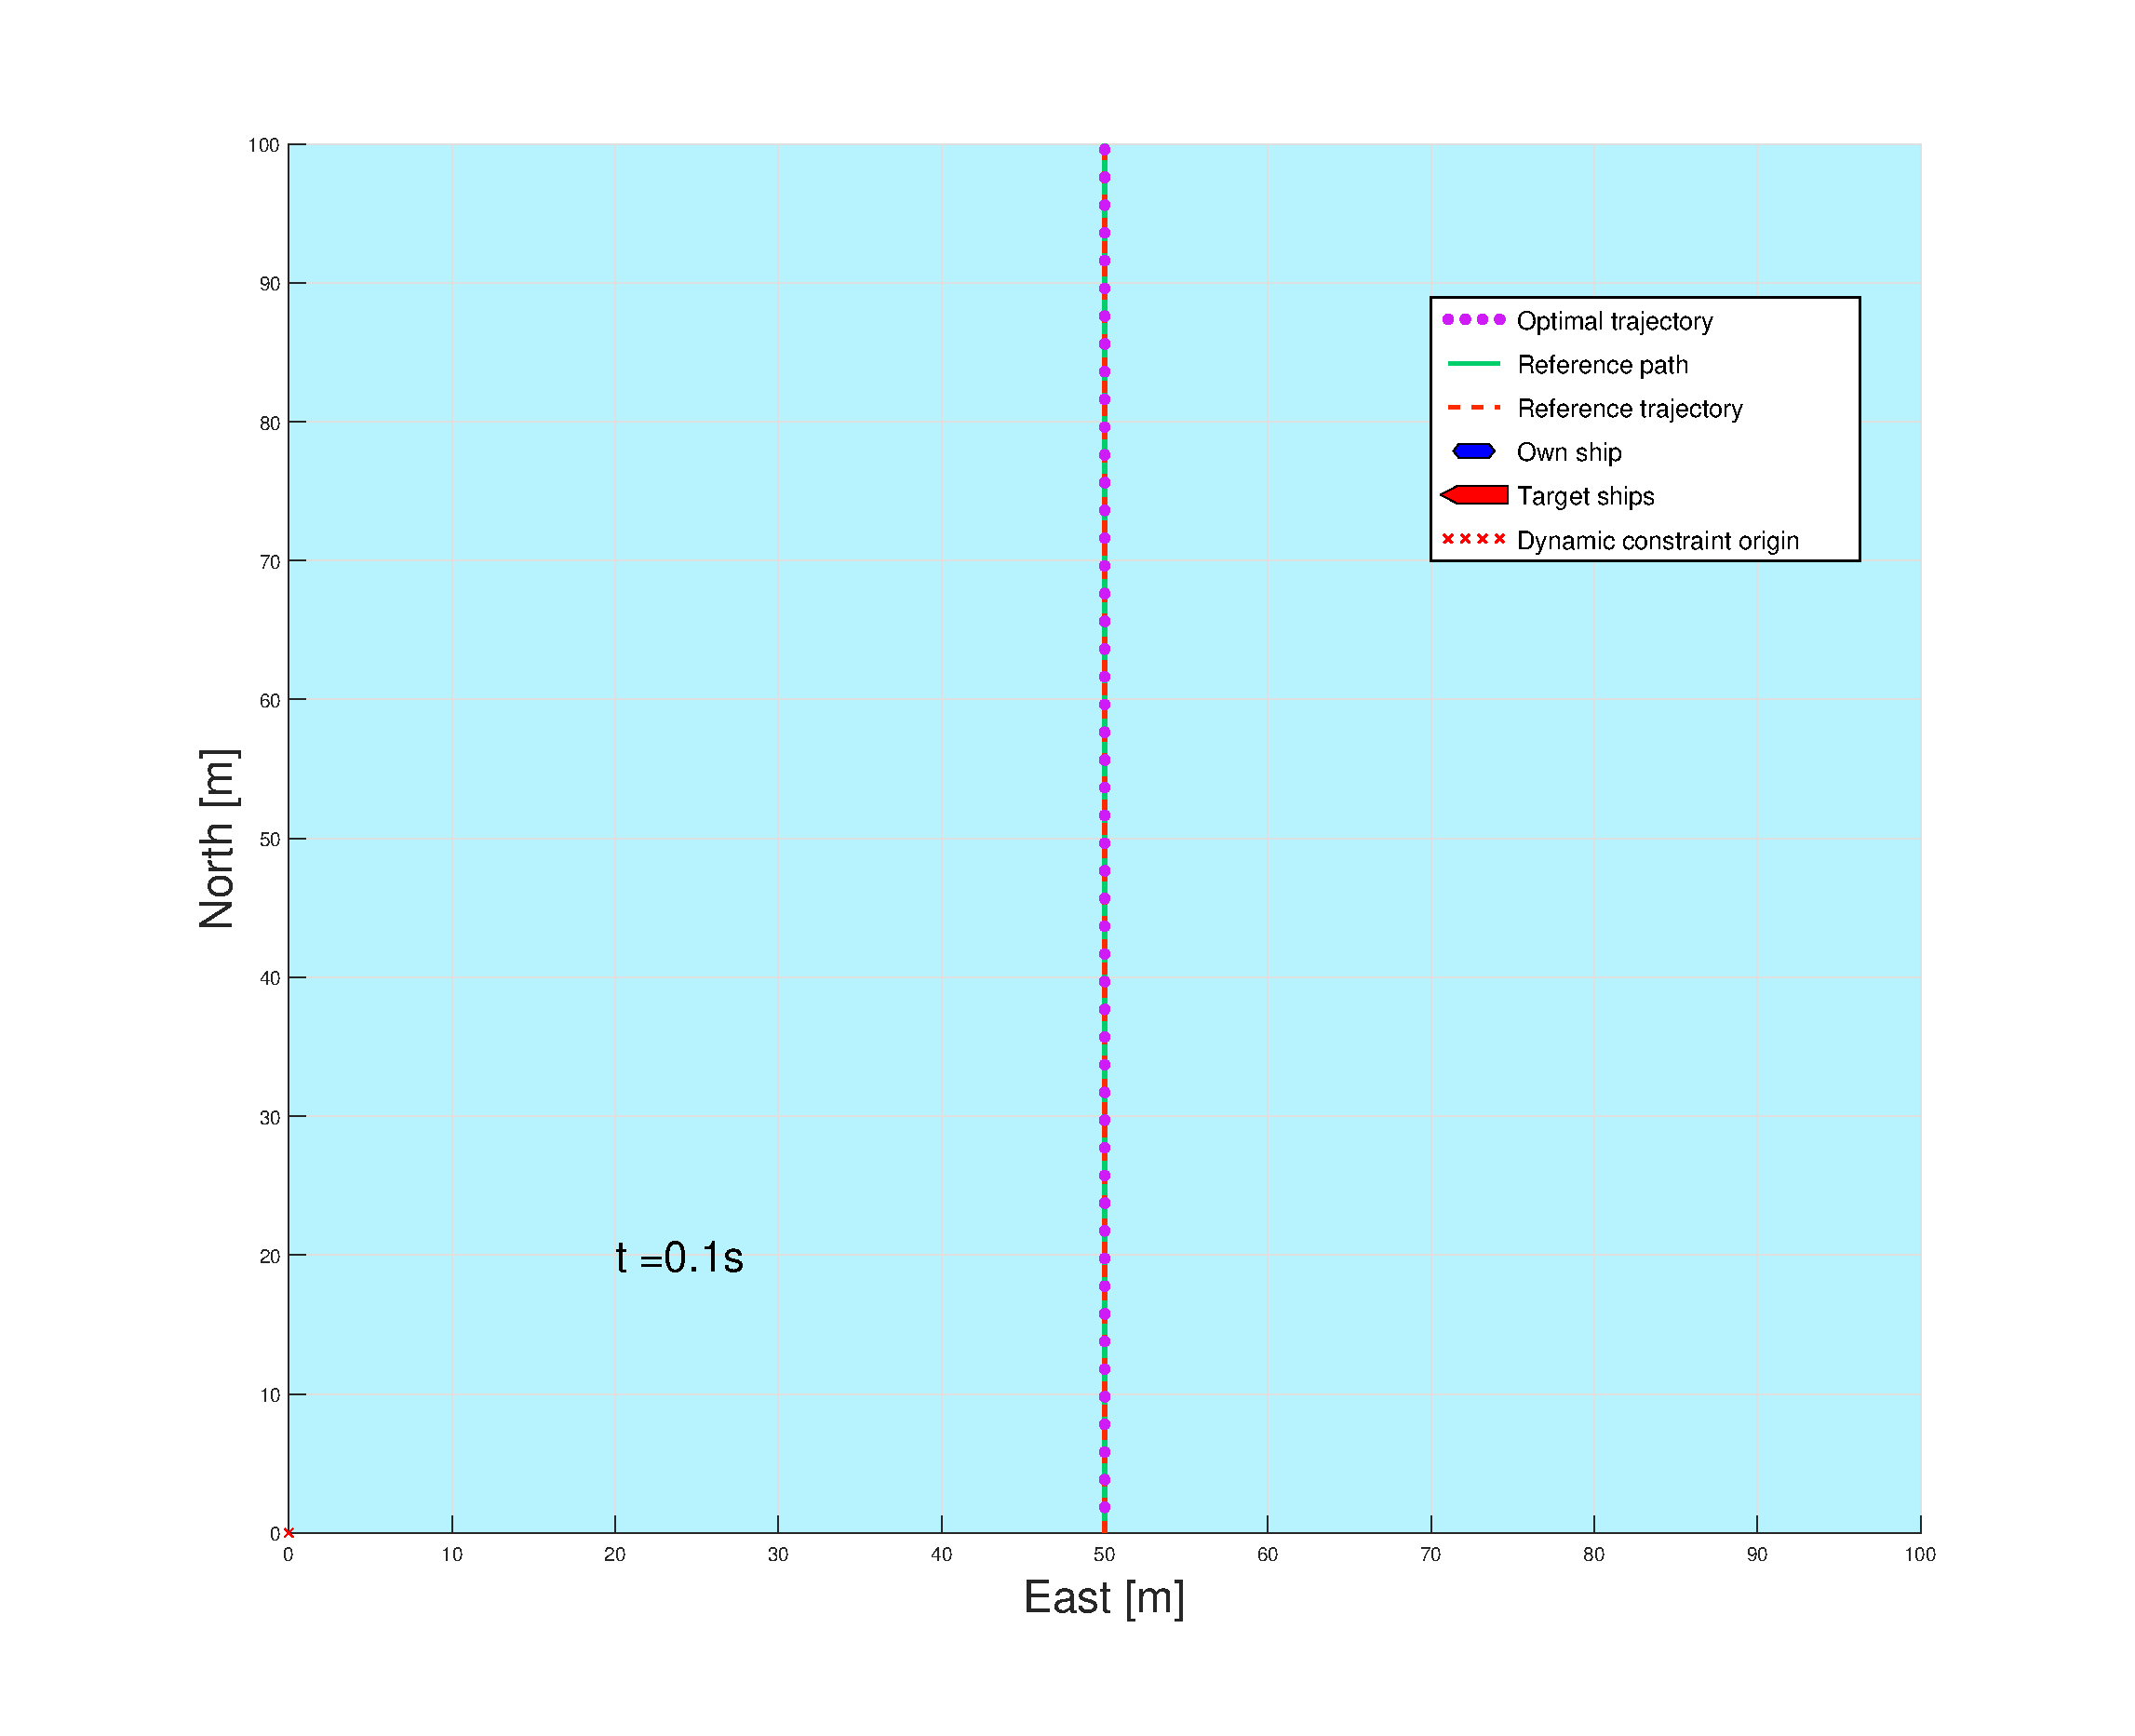
\includegraphics[width=\textwidth]{Images/Figures/enkel_GW/_Simple_0fig999_time=0}
        \subcaption{mhm}
    \end{subfigure}
    \hfill
    \\
    \begin{subfigure}[b]{0.49\textwidth}
        \centering
        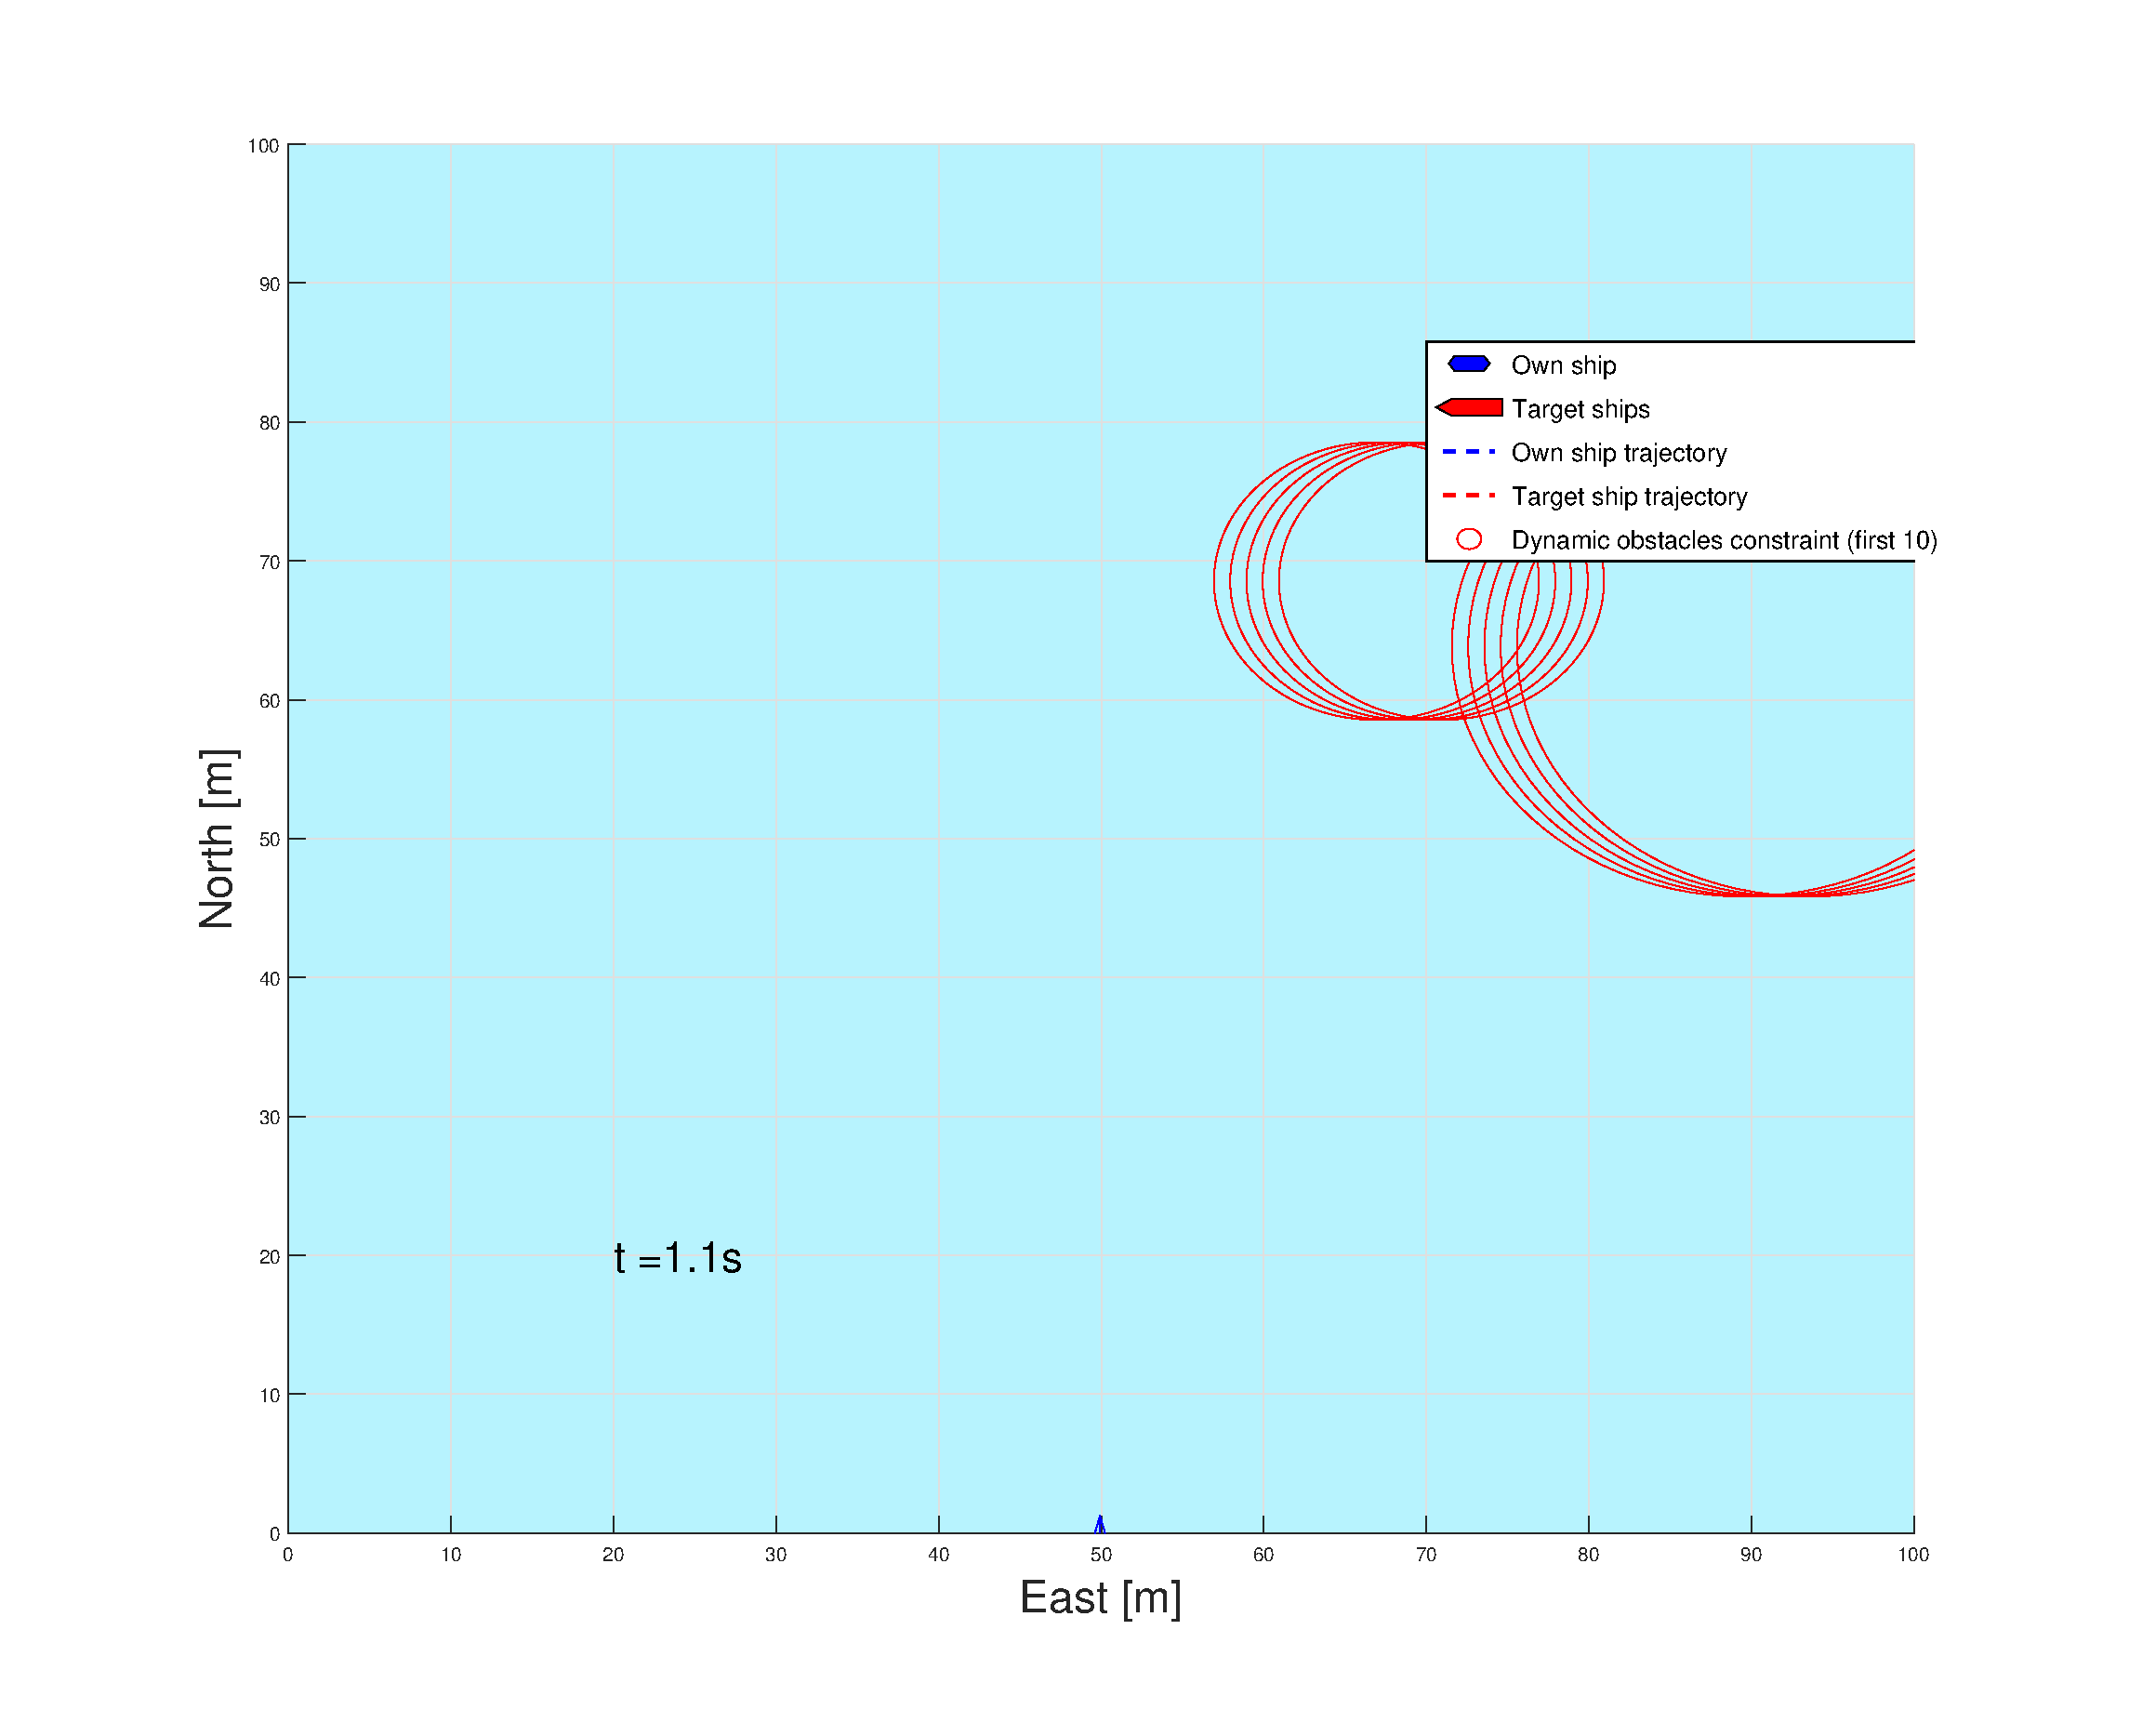
\includegraphics[width=\textwidth]{Images/Figures/enkel_GW/_Simple_0fig1_time=1}
        \subcaption{caption}
    \end{subfigure}
    \hfill
    \begin{subfigure}[b]{0.499\textwidth}
        \centering
        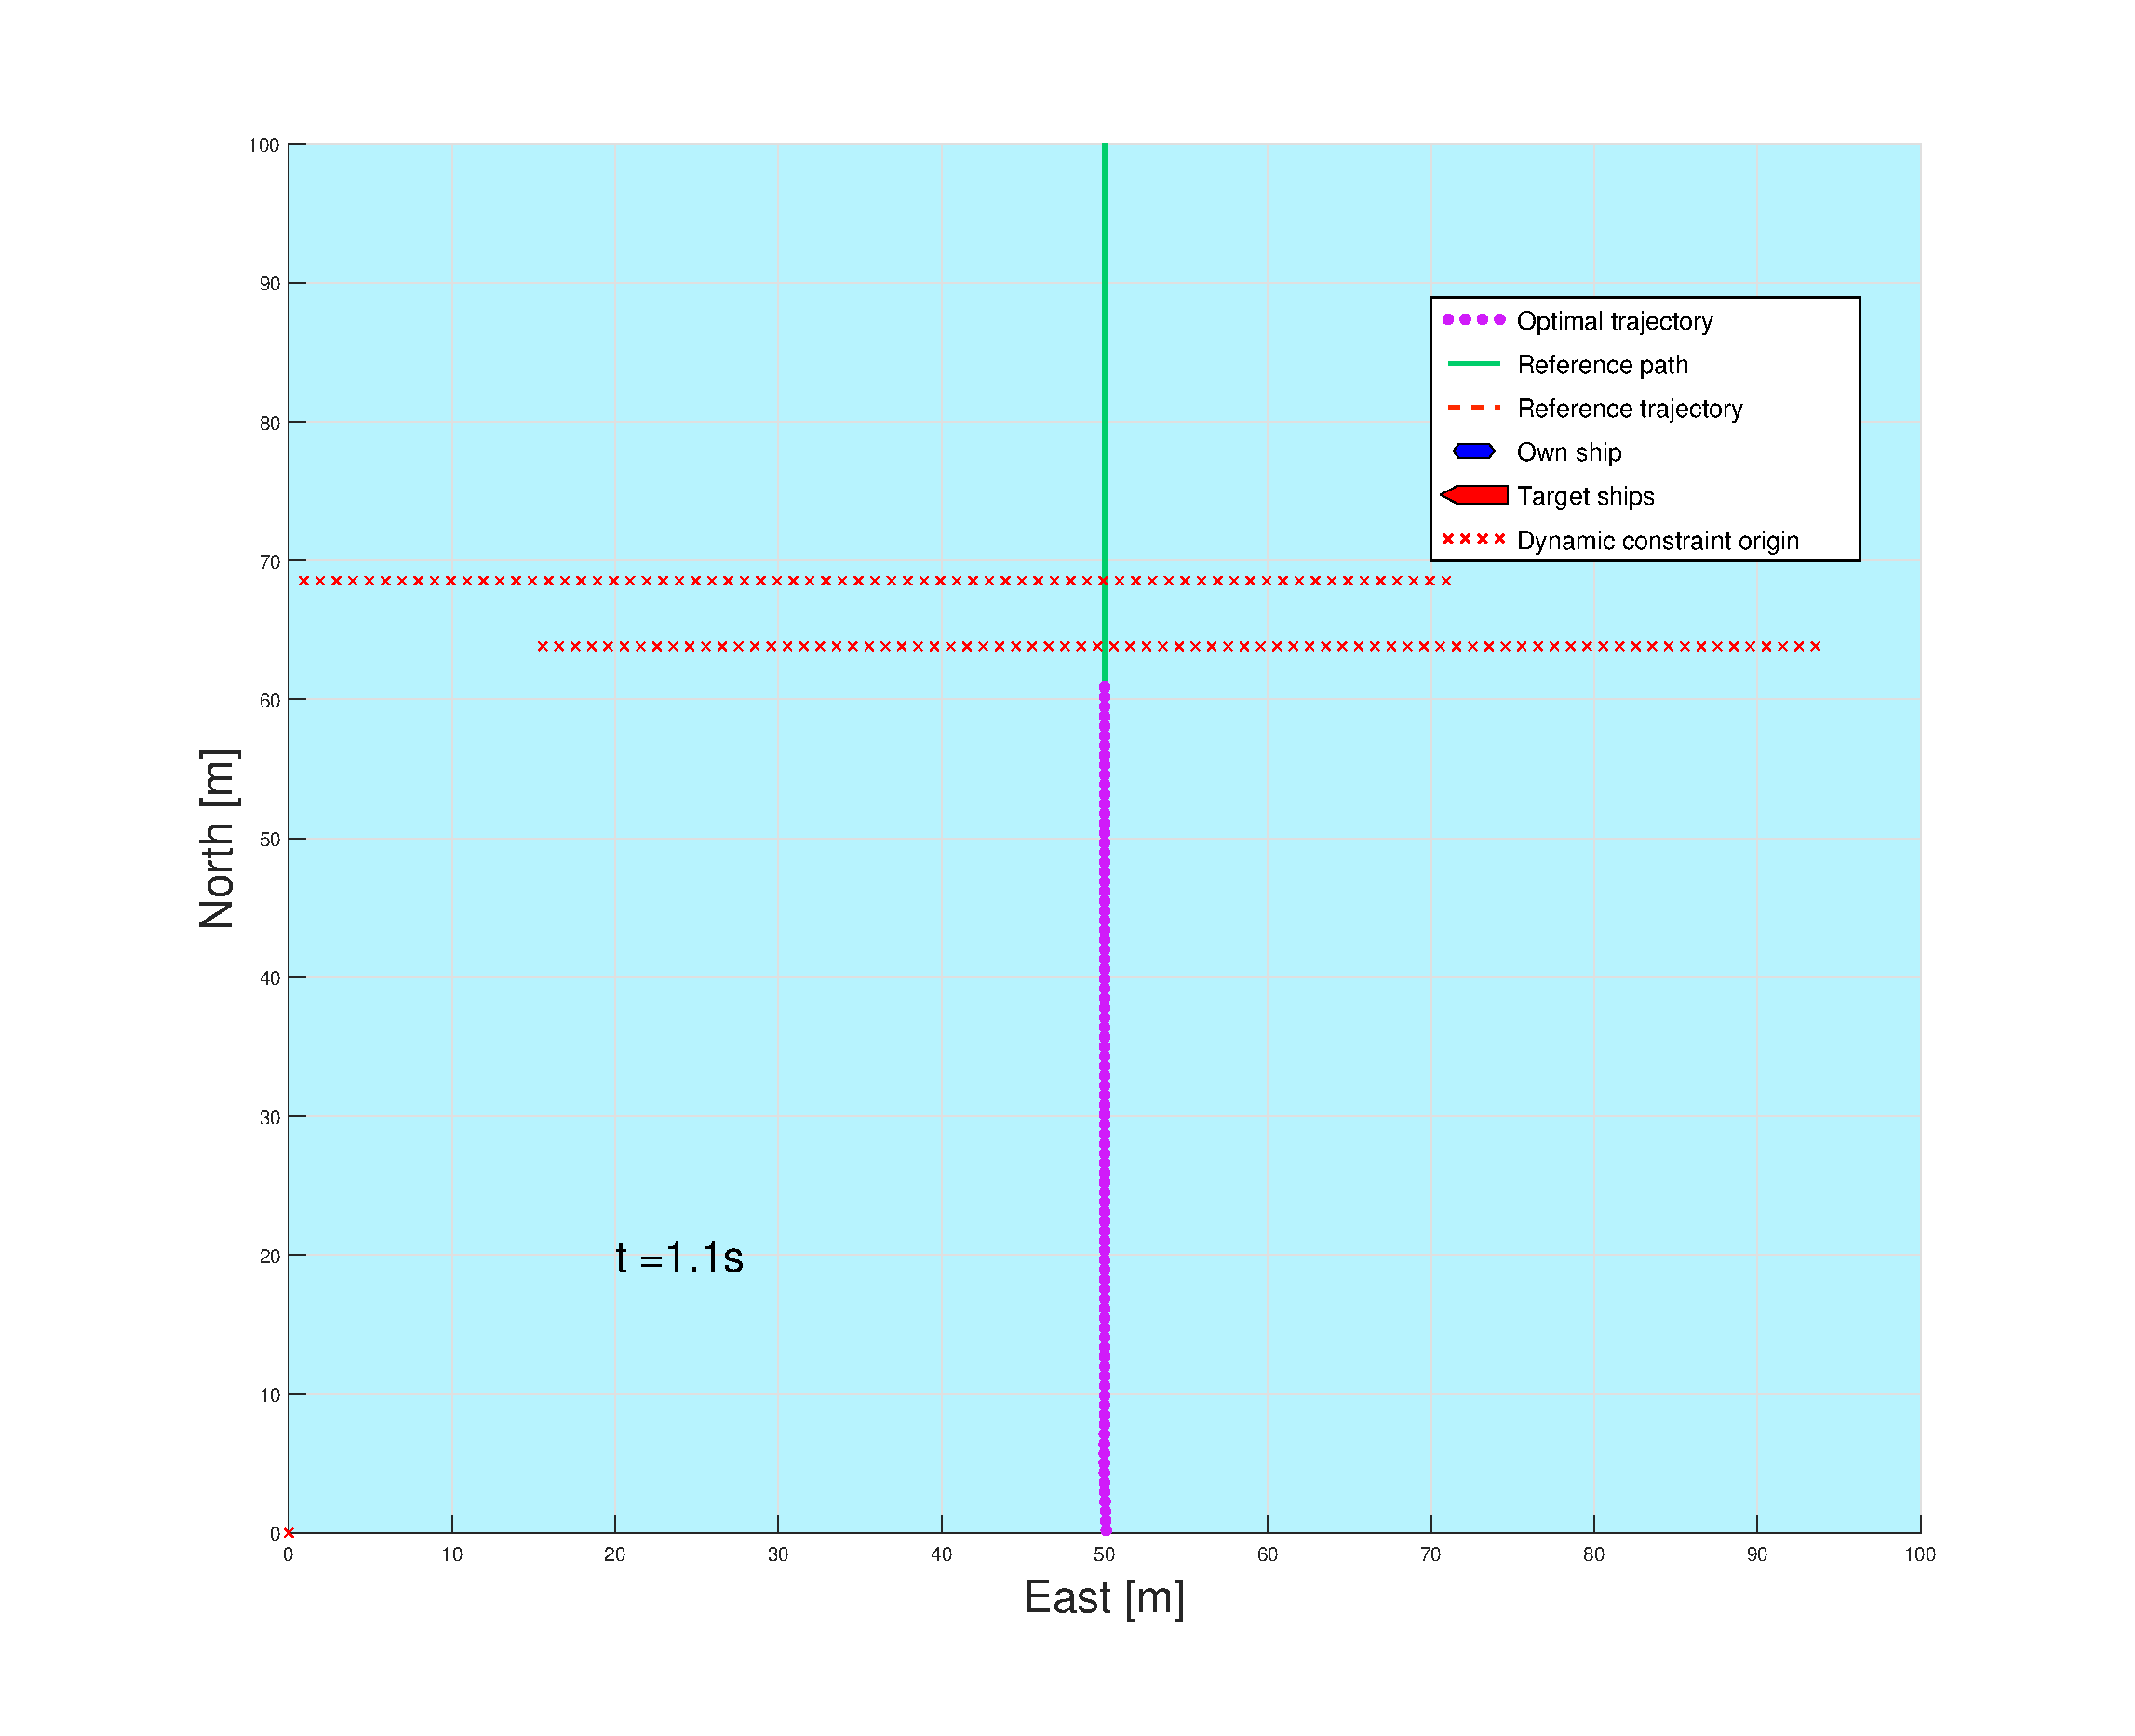
\includegraphics[width=\textwidth]{Images/Figures/enkel_GW/_Simple_0fig999_time=1}
        \subcaption{mhm}
    \end{subfigure}
    \hfill
    \\
    \begin{subfigure}[b]{0.49\textwidth}
        \centering
        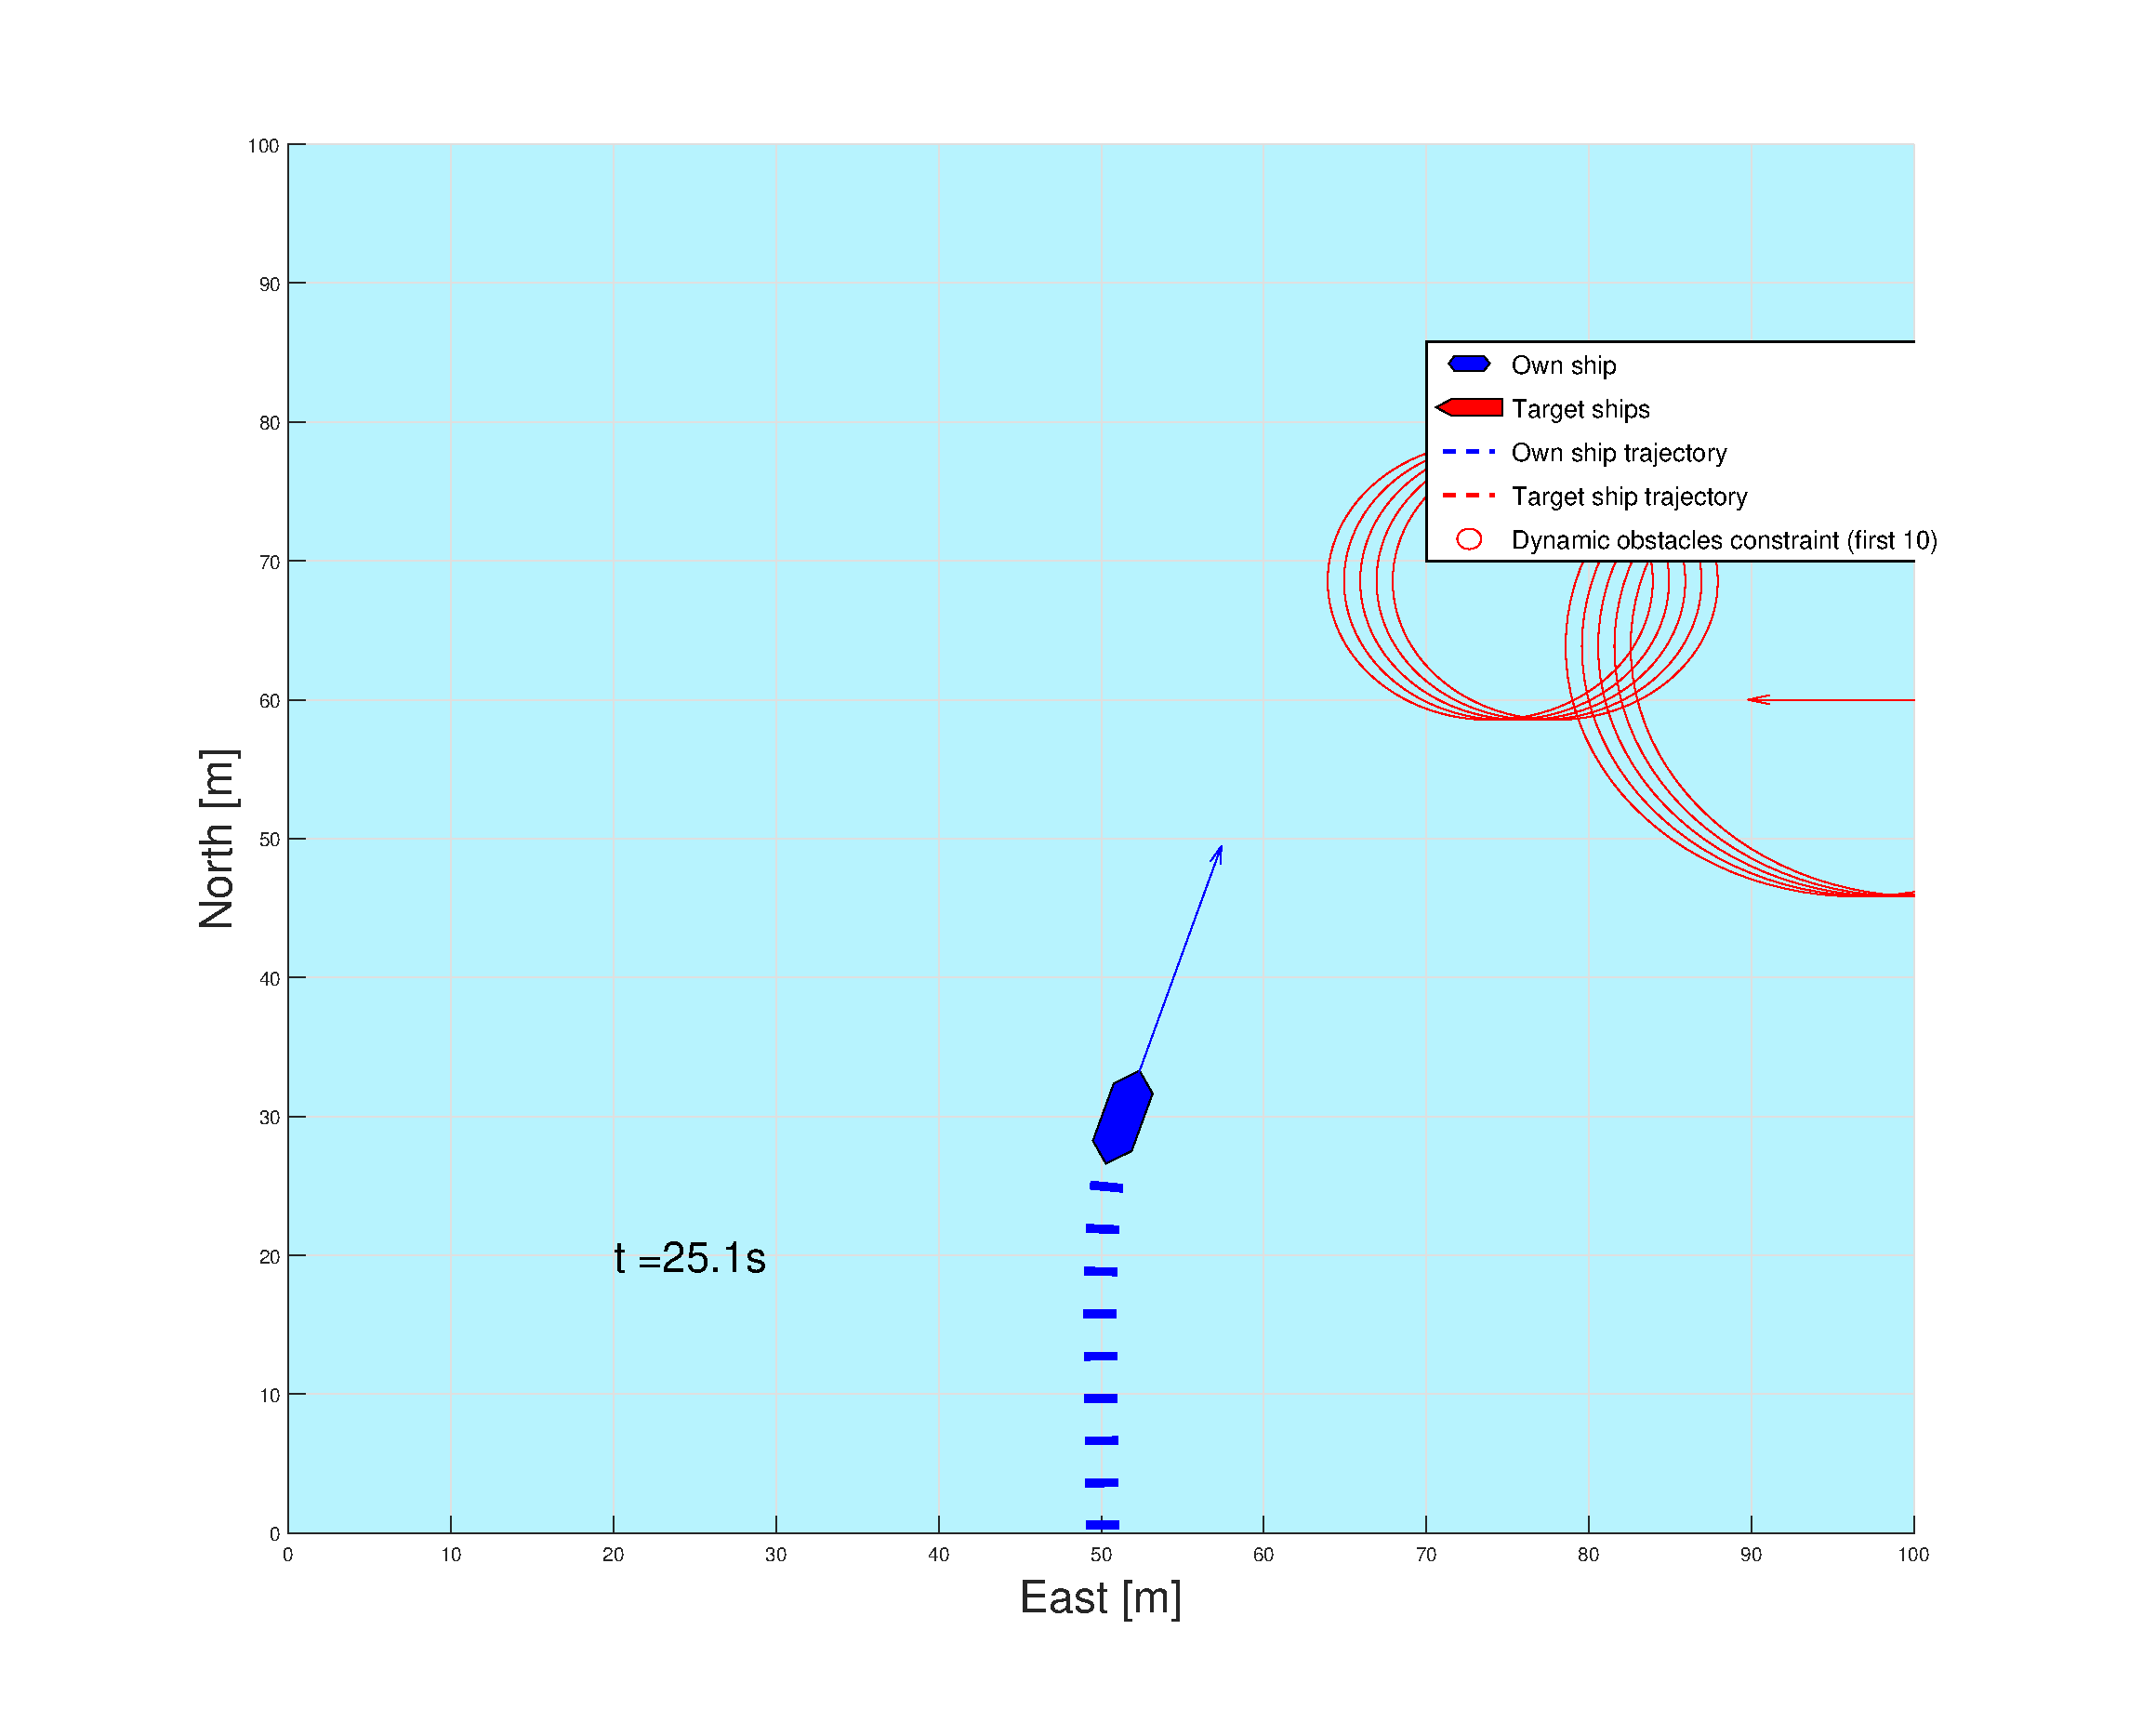
\includegraphics[width=\textwidth]{Images/Figures/enkel_GW/_Simple_0fig1_time=25}
        \subcaption{caption}
    \end{subfigure}
    \hfill
    \begin{subfigure}[b]{0.499\textwidth}
        \centering
        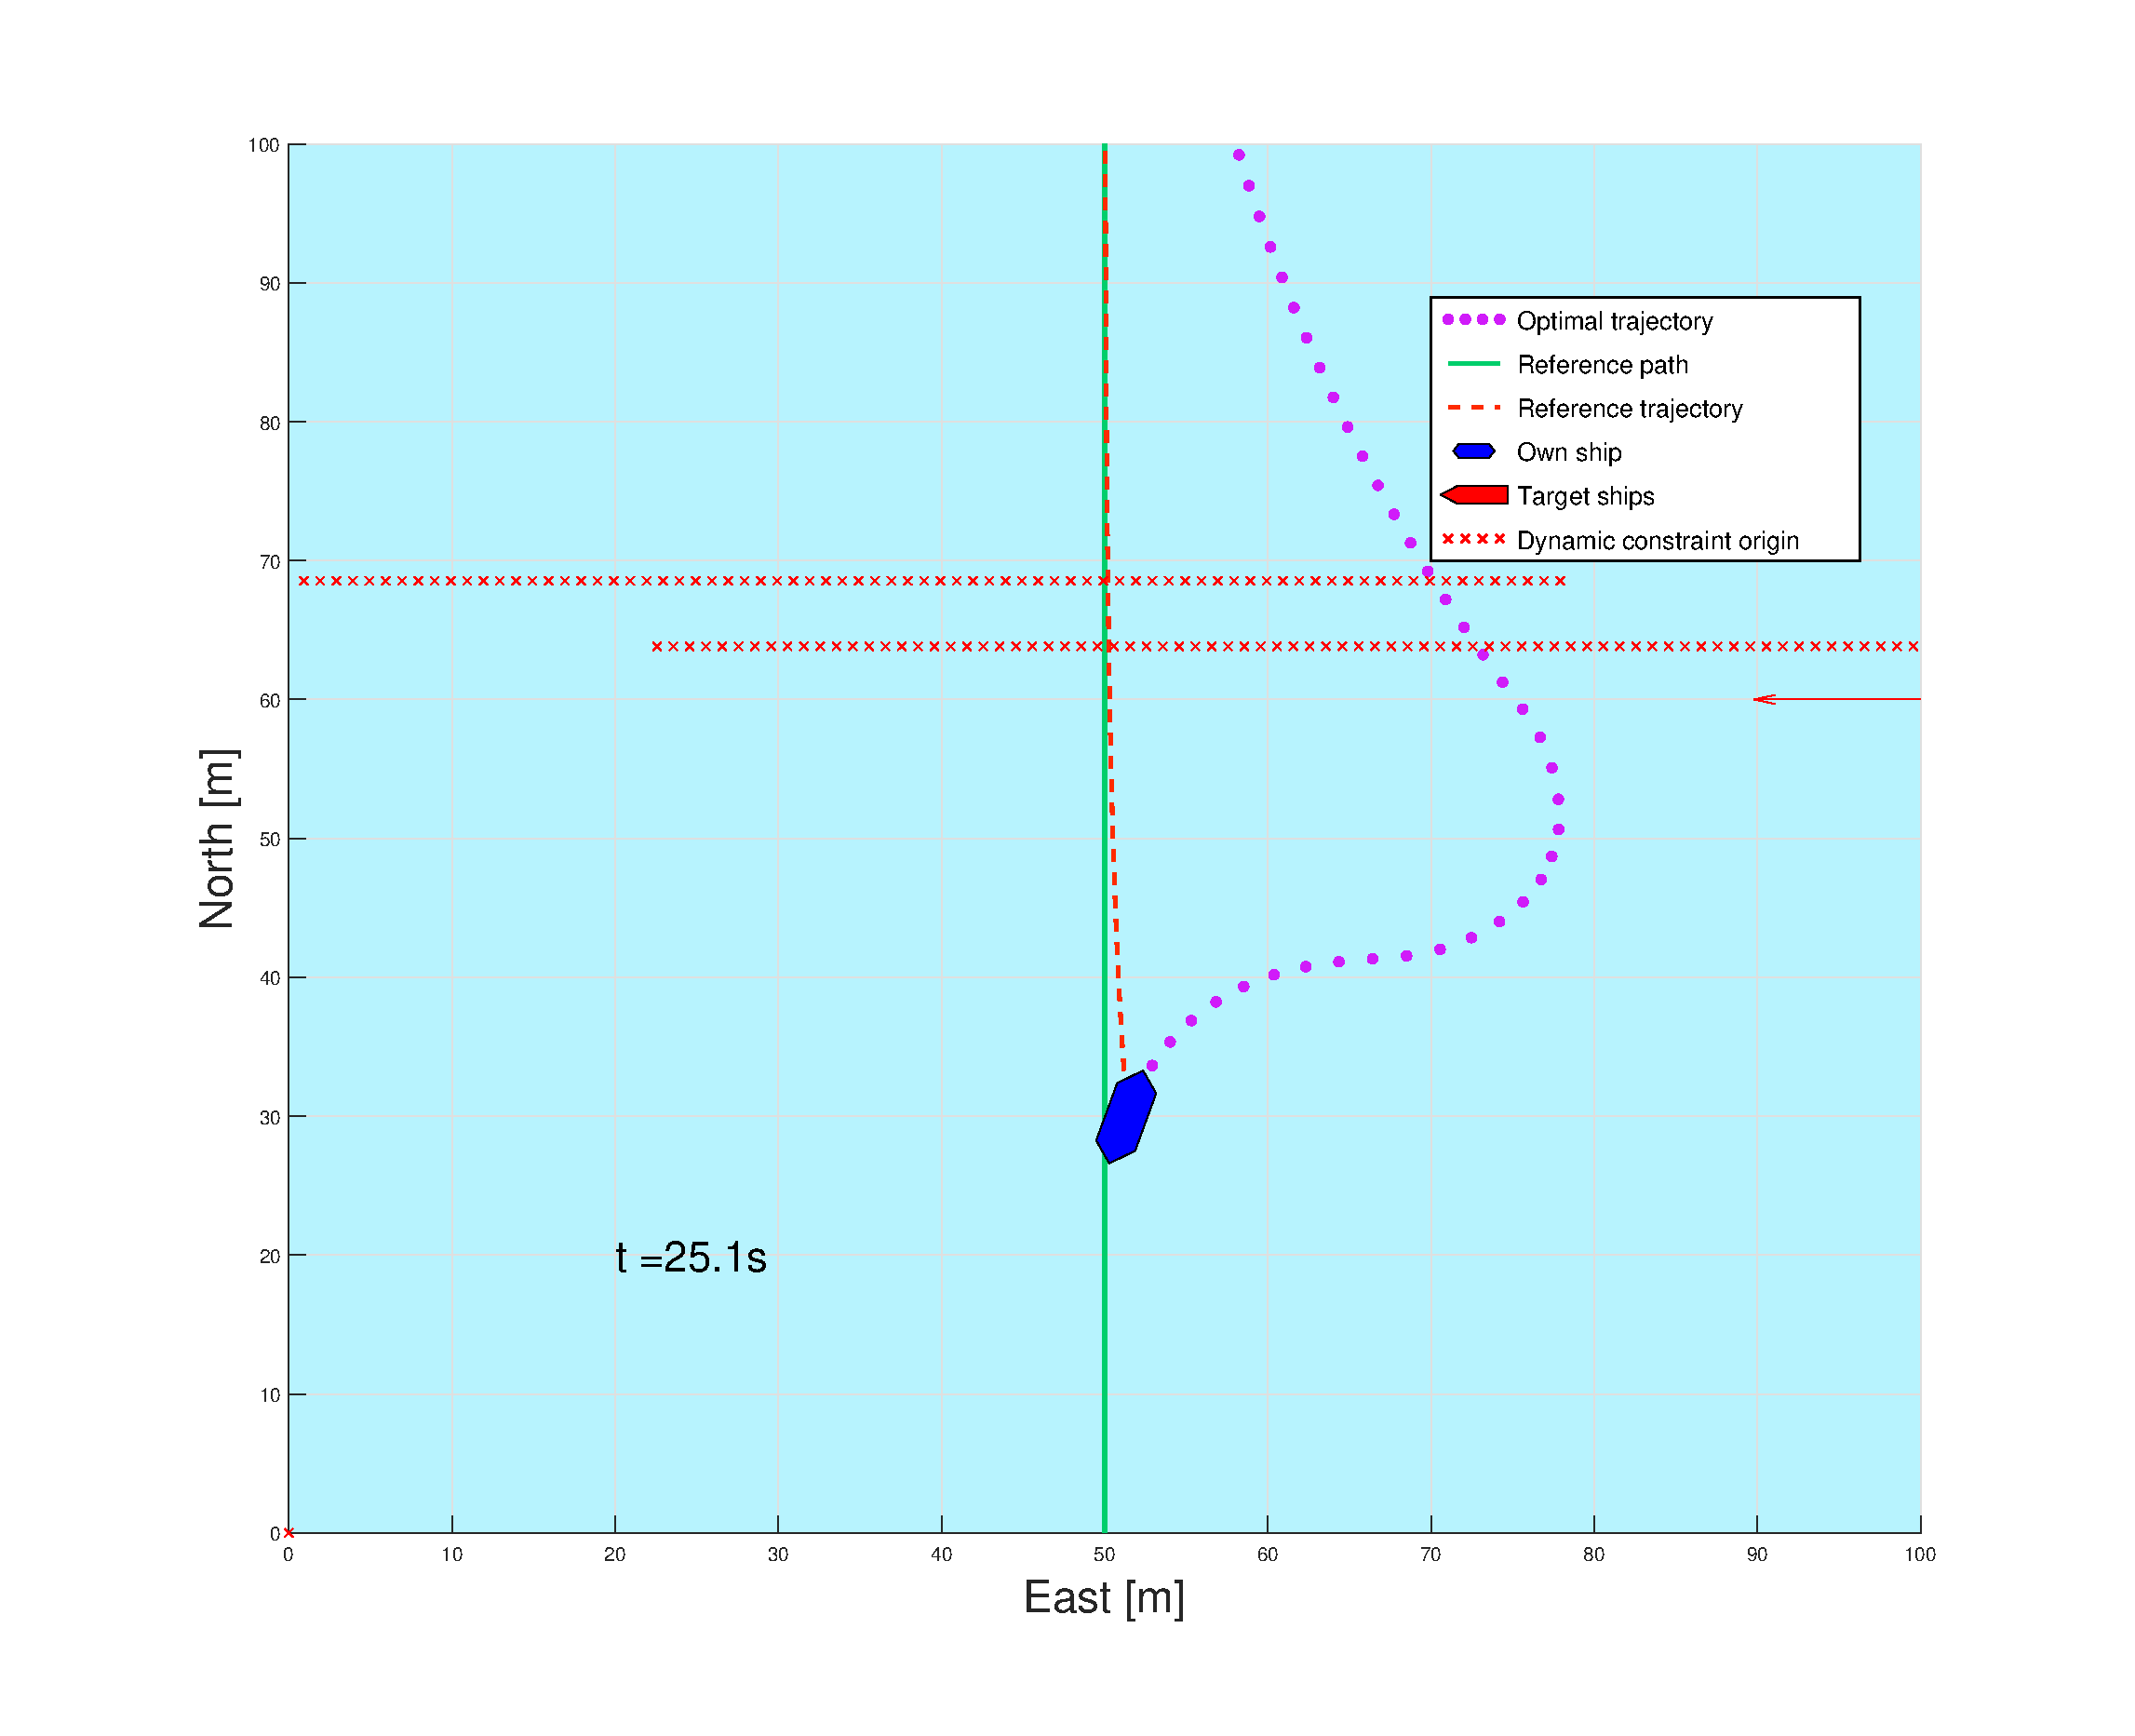
\includegraphics[width=\textwidth]{Images/Figures/enkel_GW/_Simple_0fig999_time=25}
        \subcaption{mhm}
    \end{subfigure}
    \hfill
\end{figure}%
\begin{figure}[ht]\ContinuedFloat
    \begin{subfigure}[b]{0.49\textwidth}
        \centering
        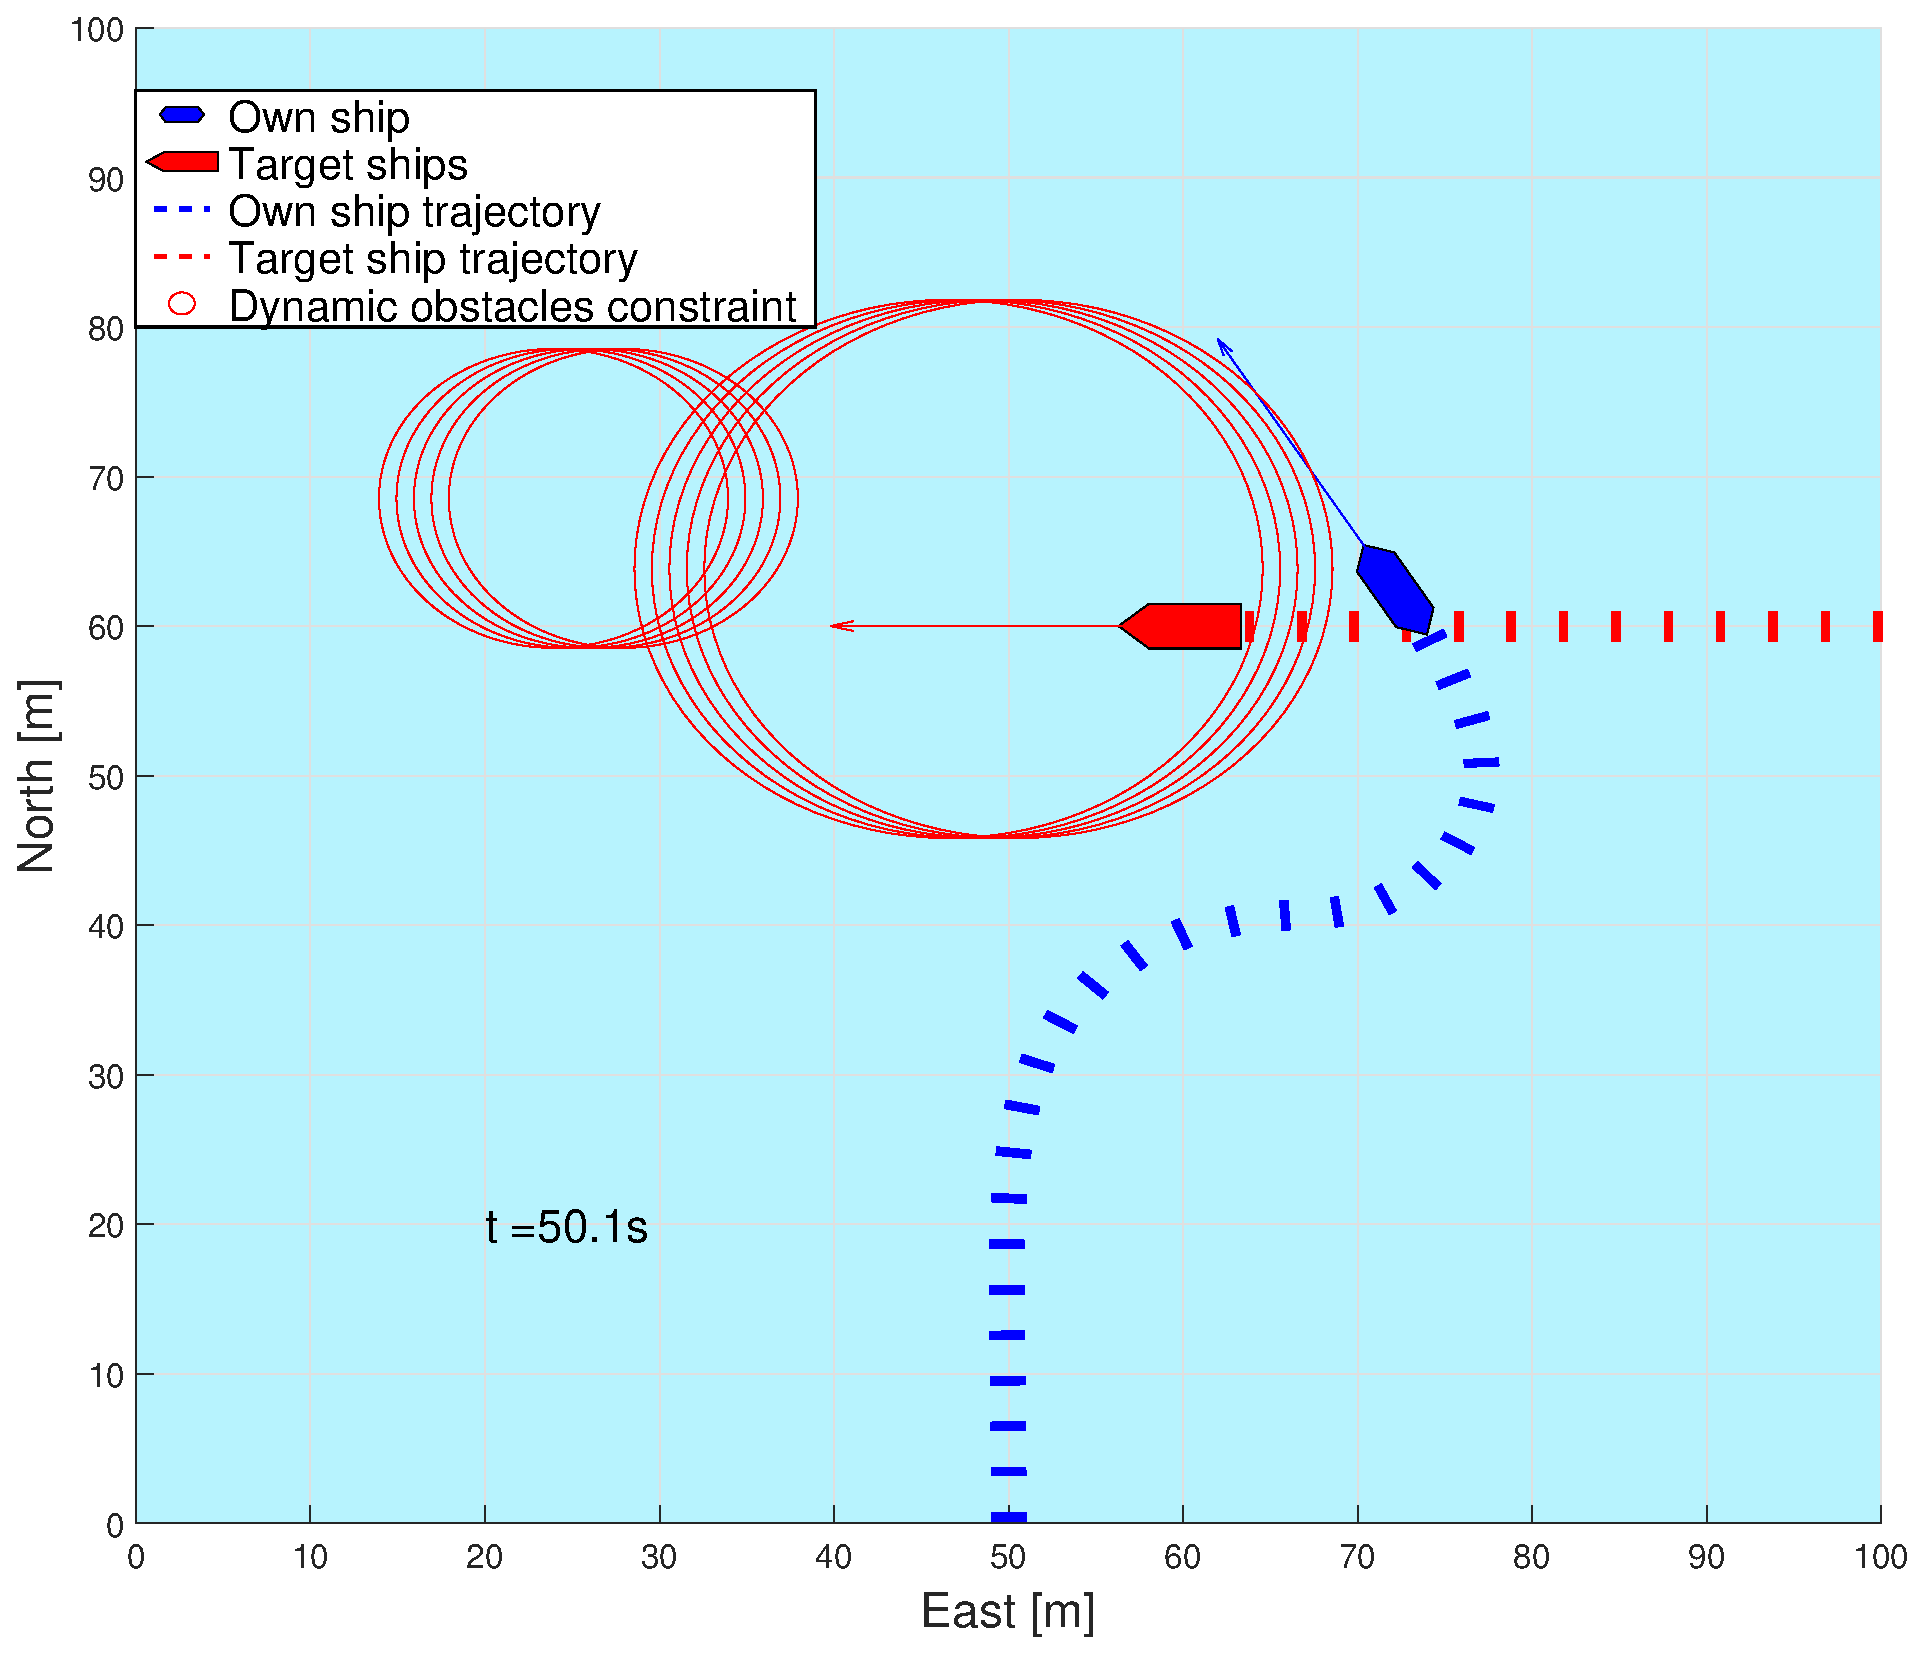
\includegraphics[width=\textwidth]{Images/Figures/enkel_GW/_Simple_0fig1_time=50}
        \subcaption{caption}
    \end{subfigure}
    \hfill
    \begin{subfigure}[b]{0.499\textwidth}
        \centering
        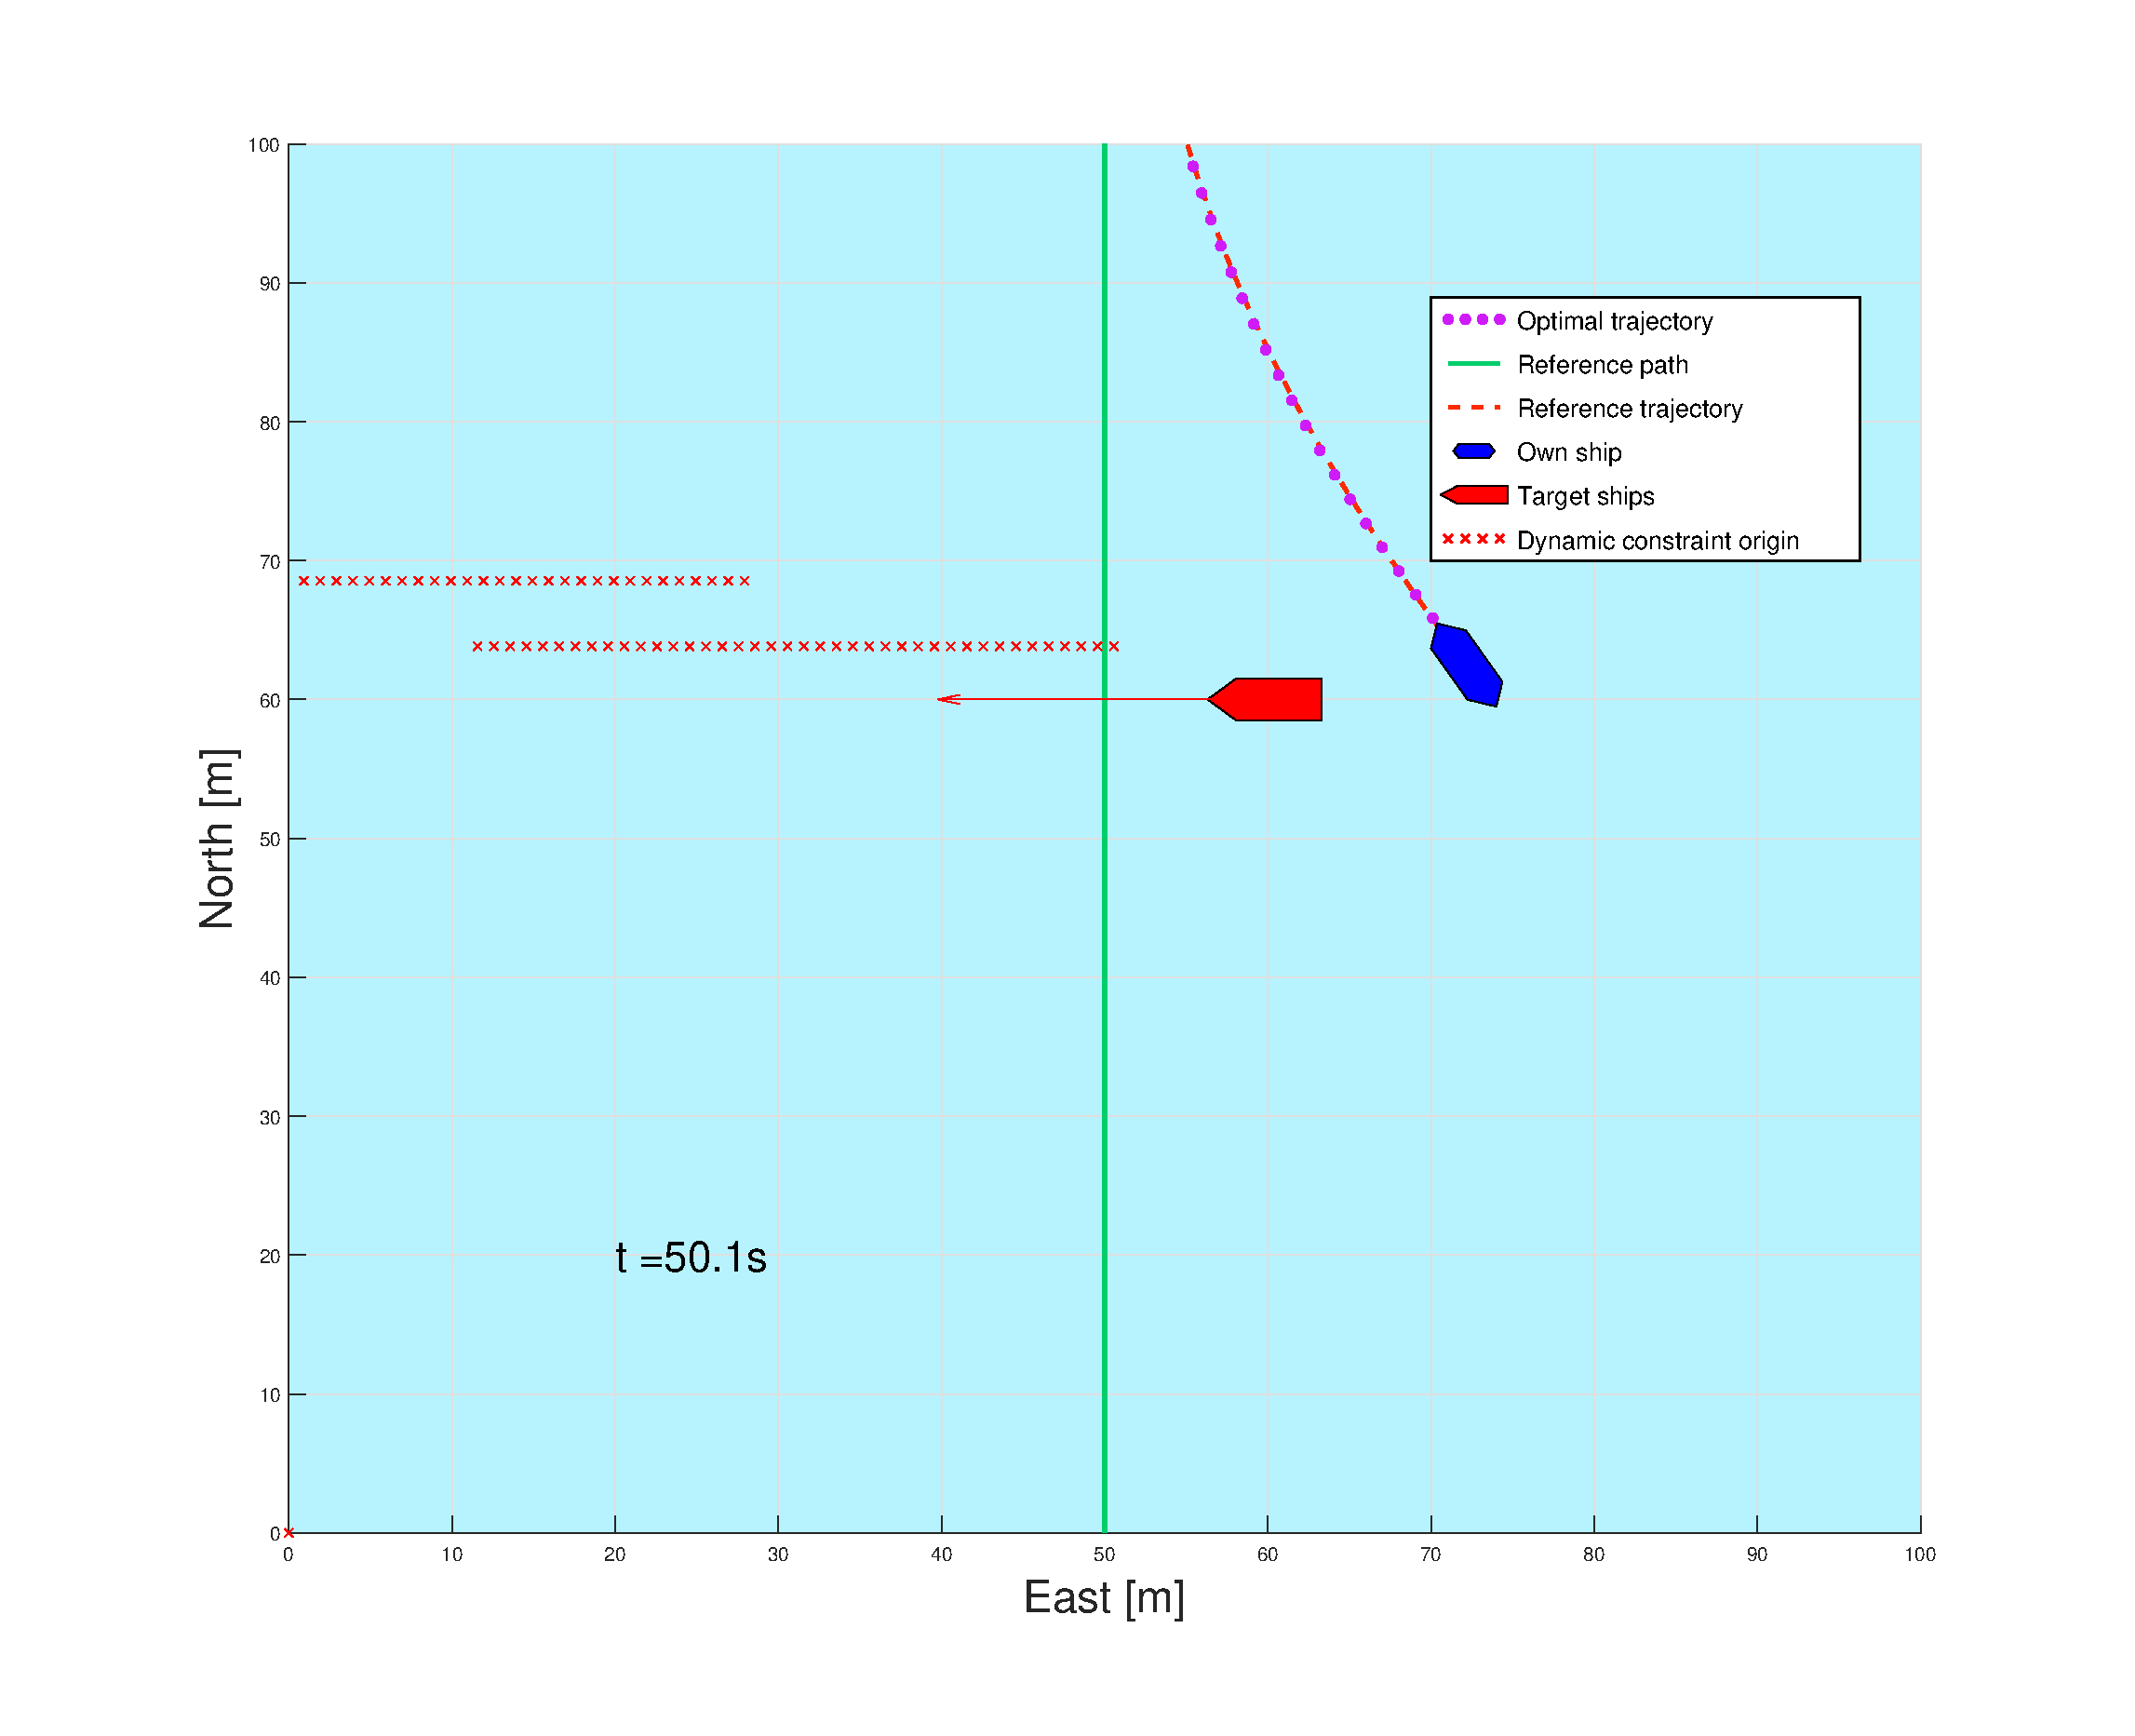
\includegraphics[width=\textwidth]{Images/Figures/enkel_GW/_Simple_0fig999_time=50}
        \subcaption{mhm}
    \end{subfigure}
    \hfill
    \\
    \begin{subfigure}[b]{0.49\textwidth}
        \centering
        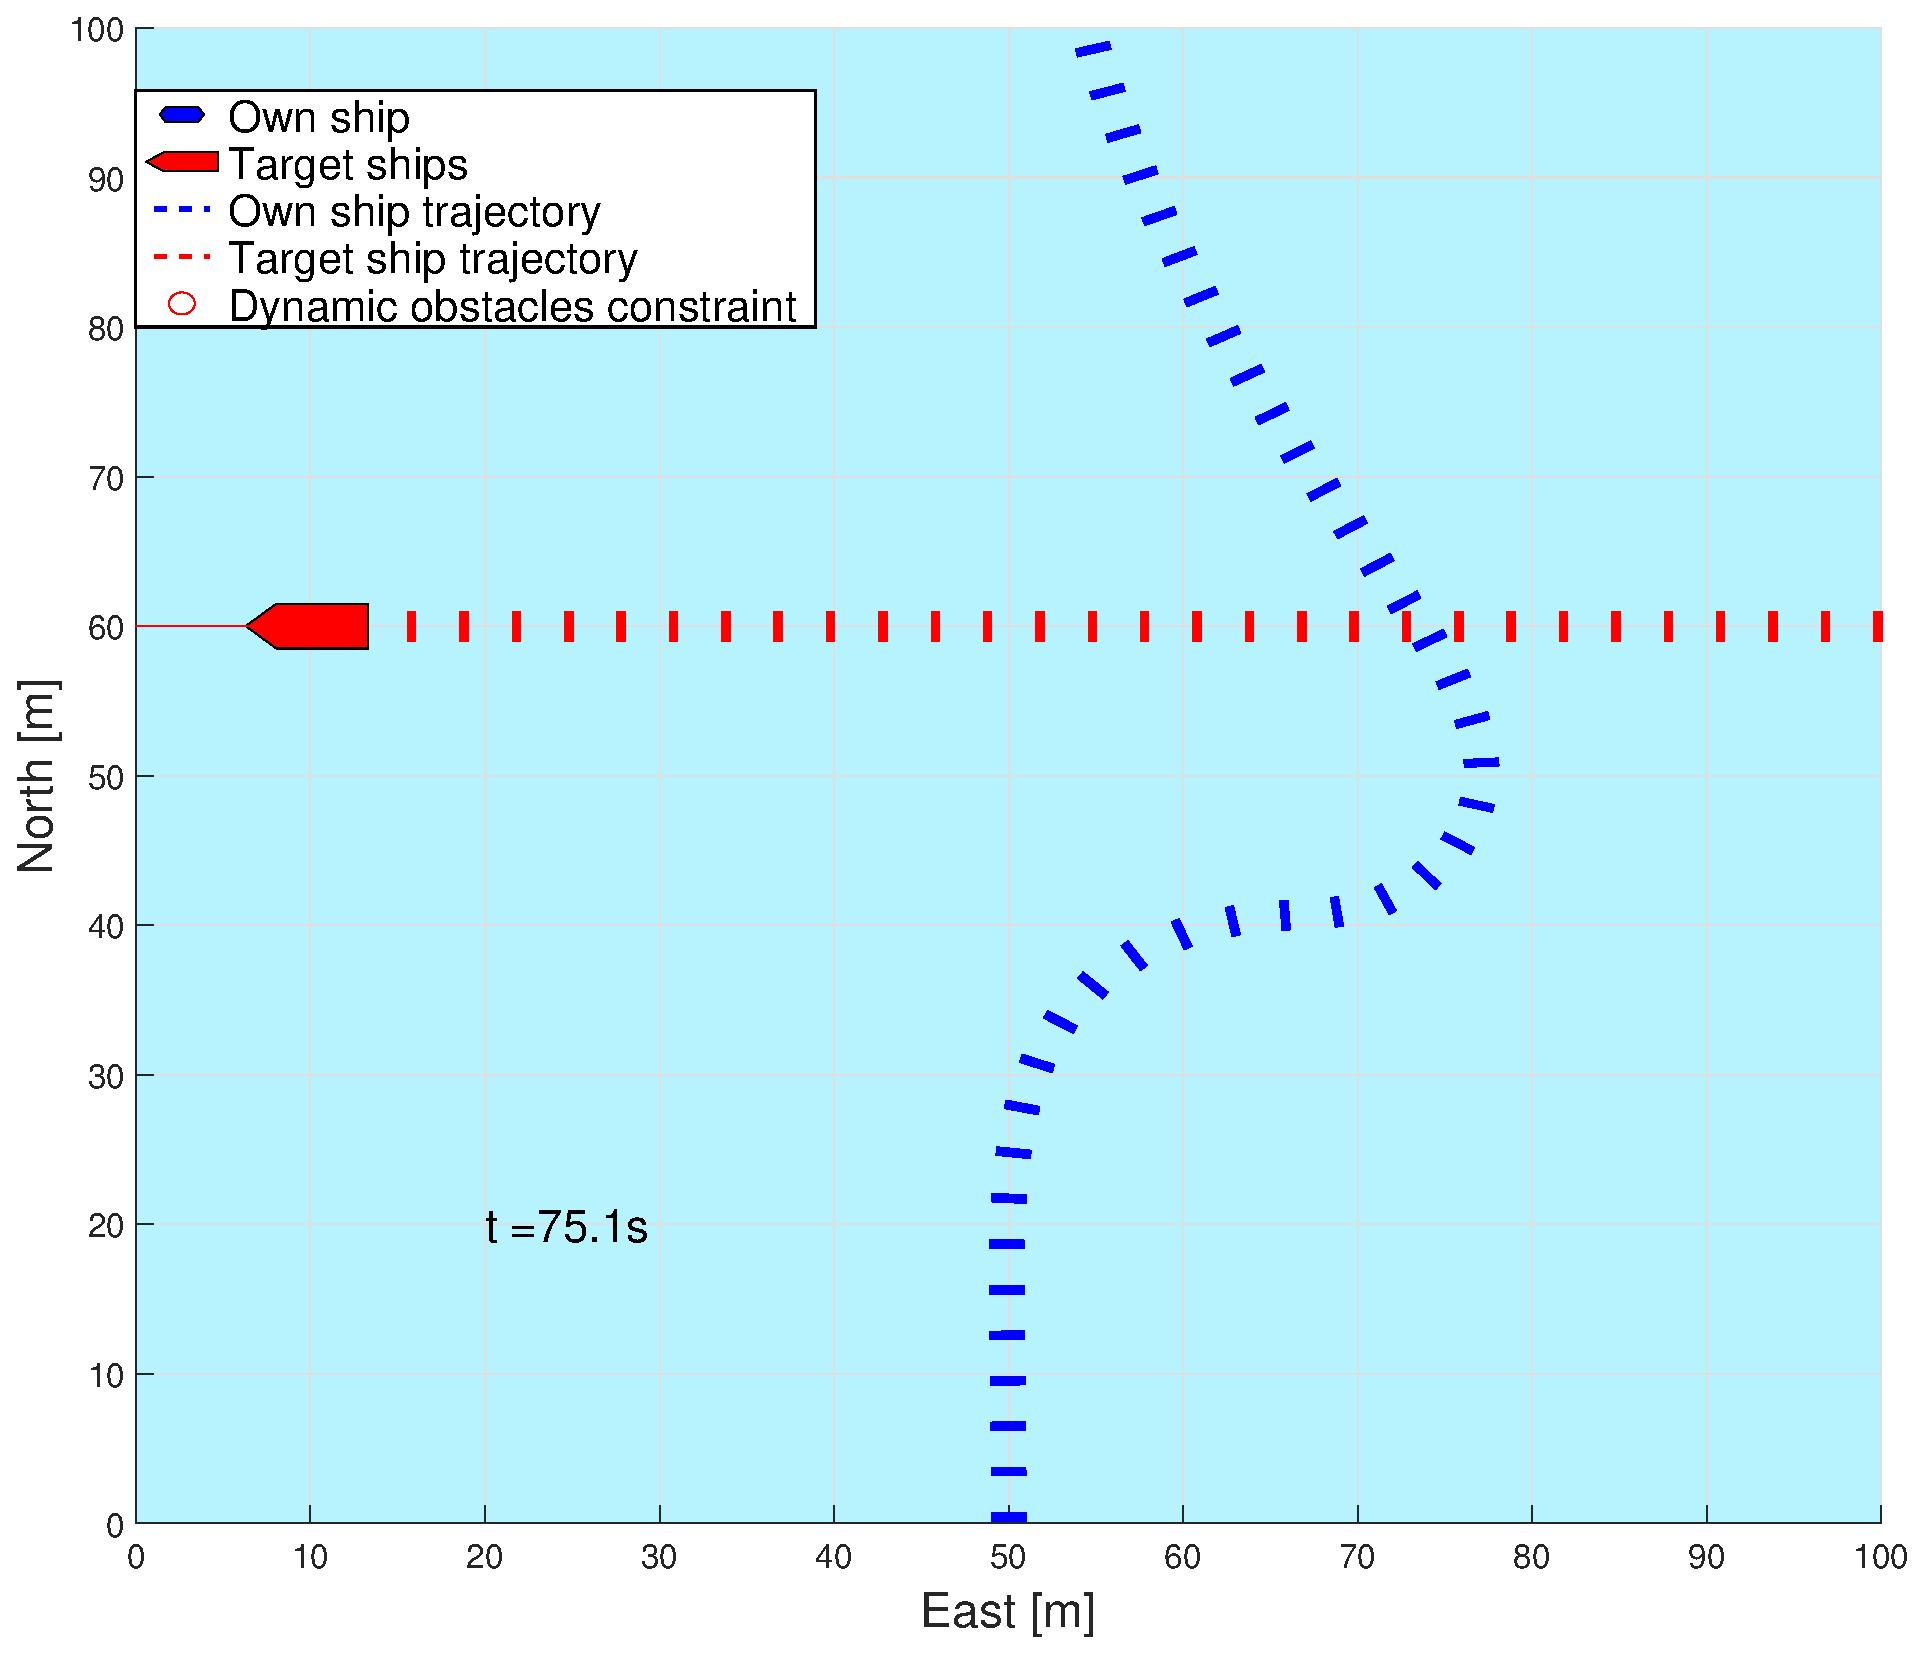
\includegraphics[width=\textwidth]{Images/Figures/enkel_GW/_Simple_0fig1_time=75}
        \subcaption{caption}
    \end{subfigure}
    \hfill
    \begin{subfigure}[b]{0.499\textwidth}
        \centering
        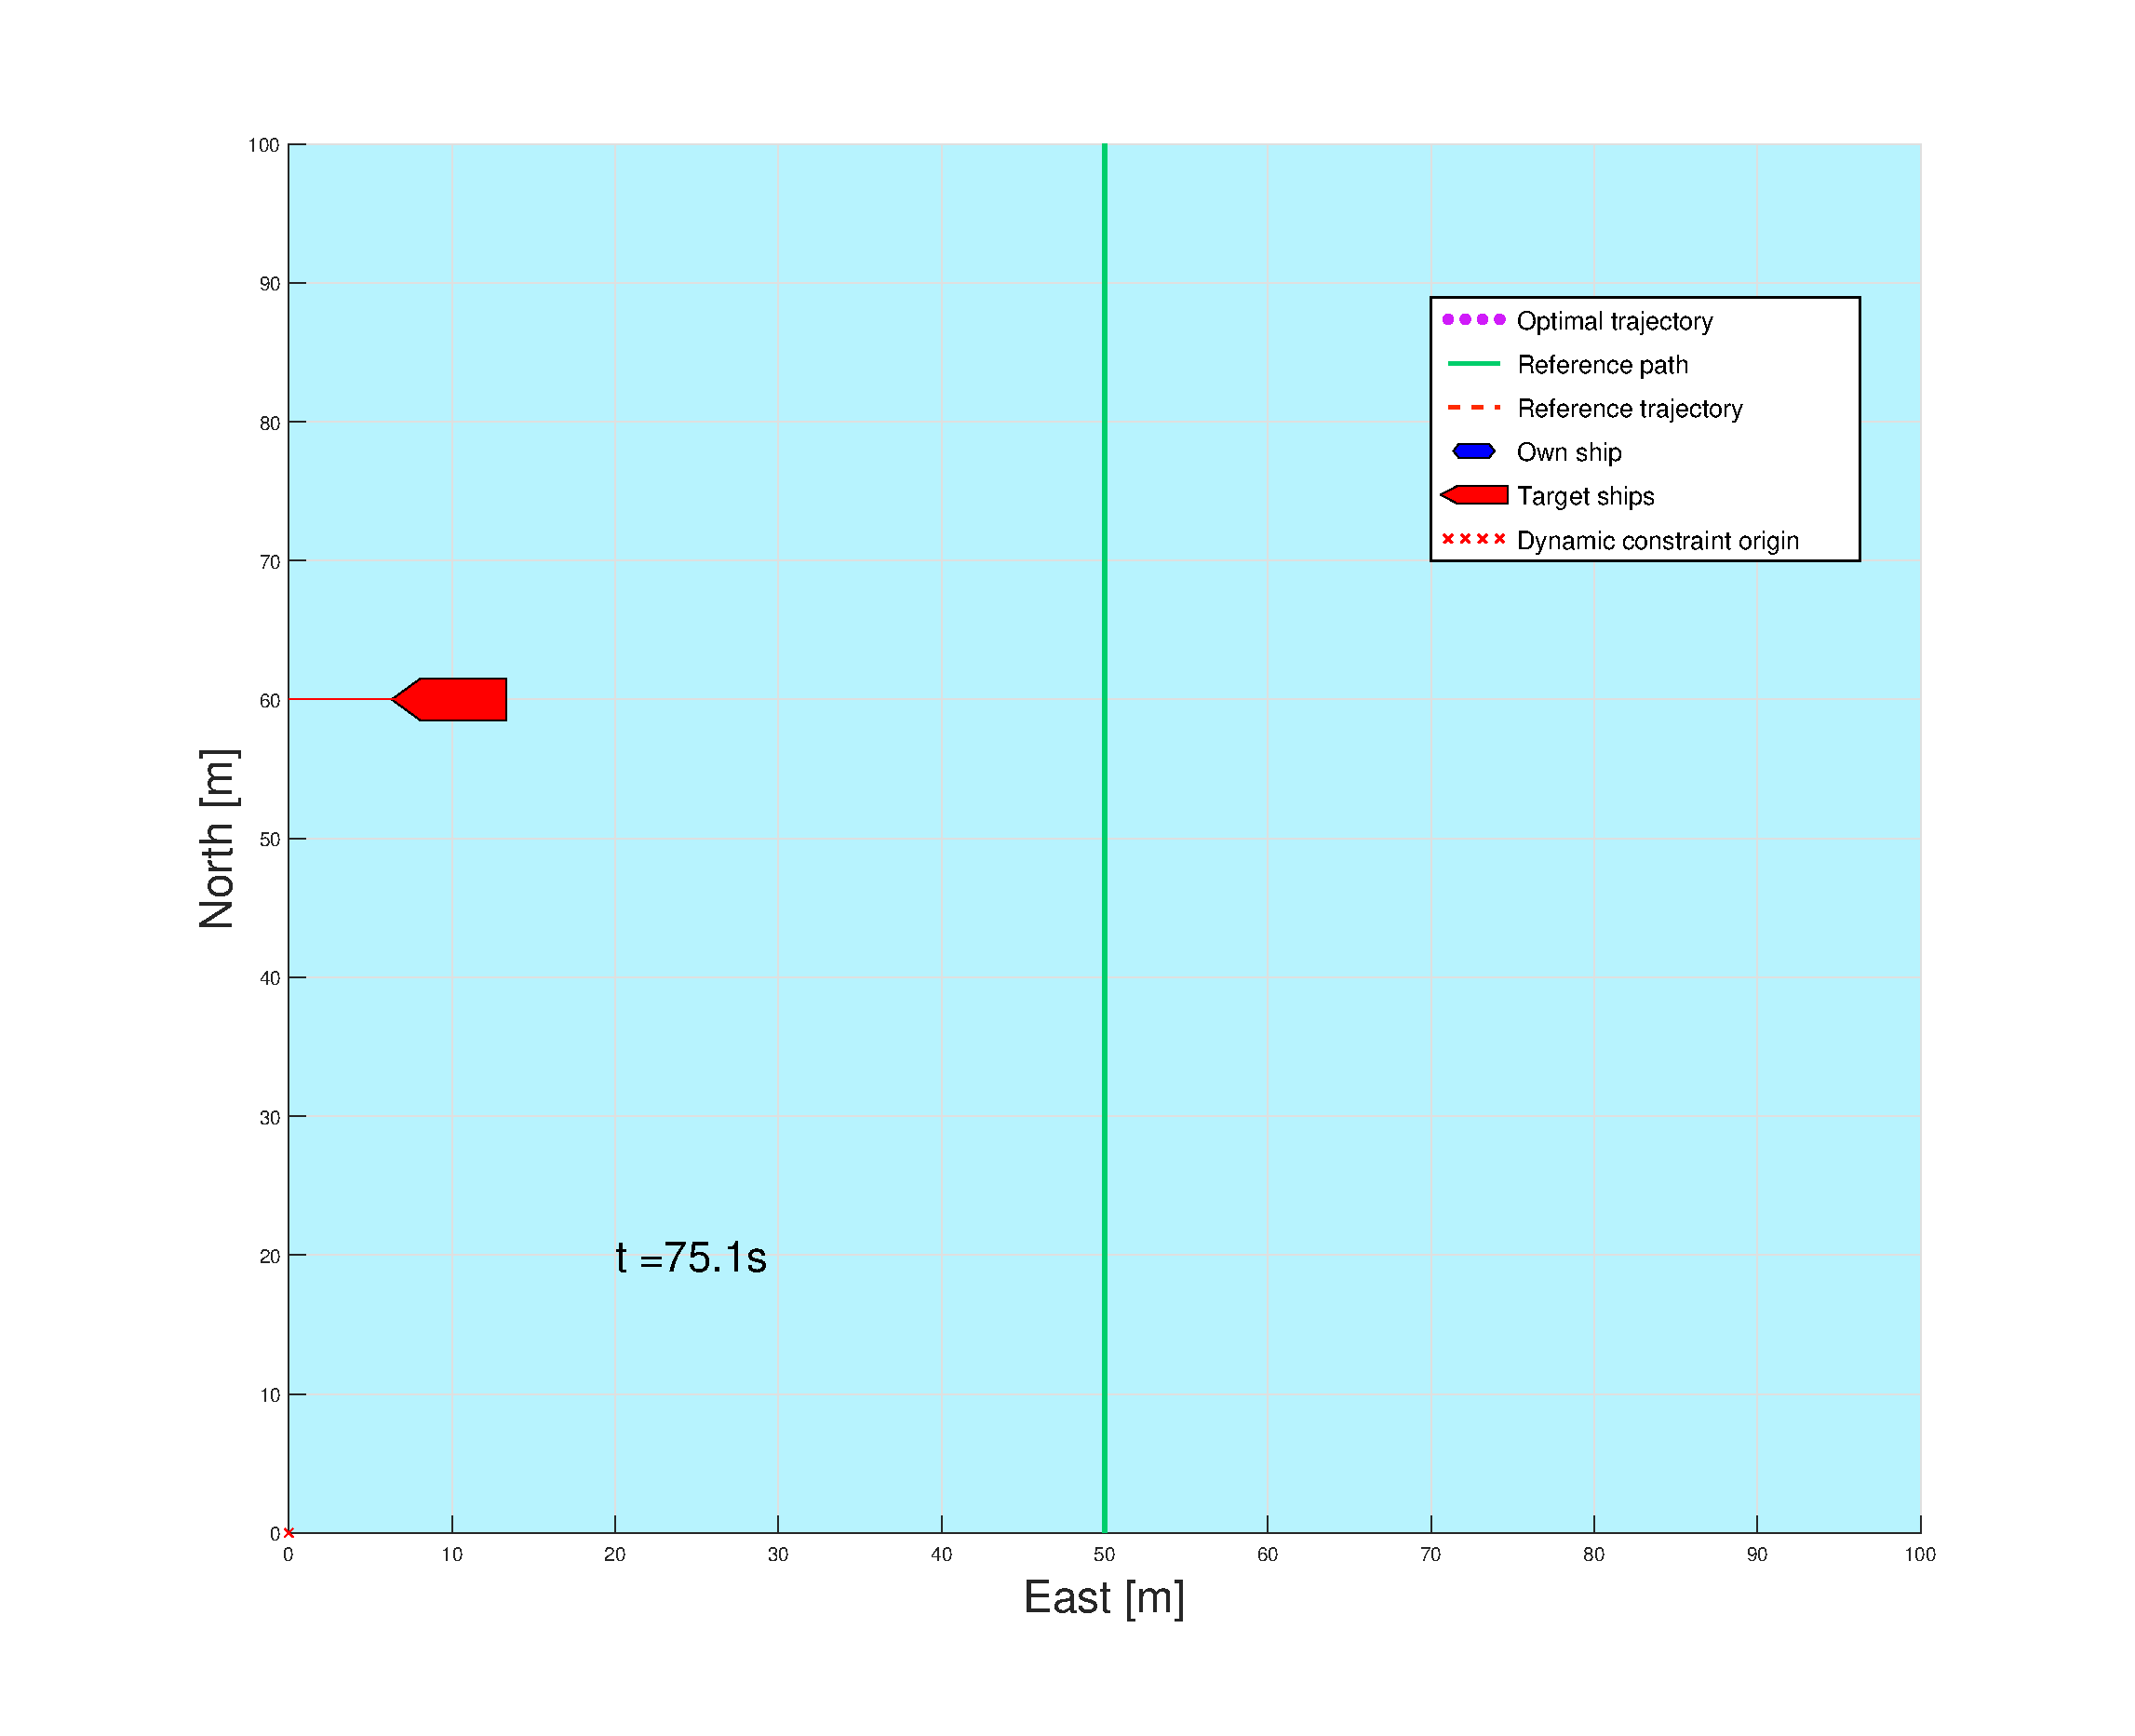
\includegraphics[width=\textwidth]{Images/Figures/enkel_GW/_Simple_0fig999_time=75}
        \subcaption{mhm}
    \end{subfigure}
    \hfill
    \caption{Simple Give Way With Prediction}
\end{figure}

\begin{figure}[!b] %Canals simulation, shown with and without constraints
    \begin{subfigure}[b]{0.49\textwidth}
        \centering
        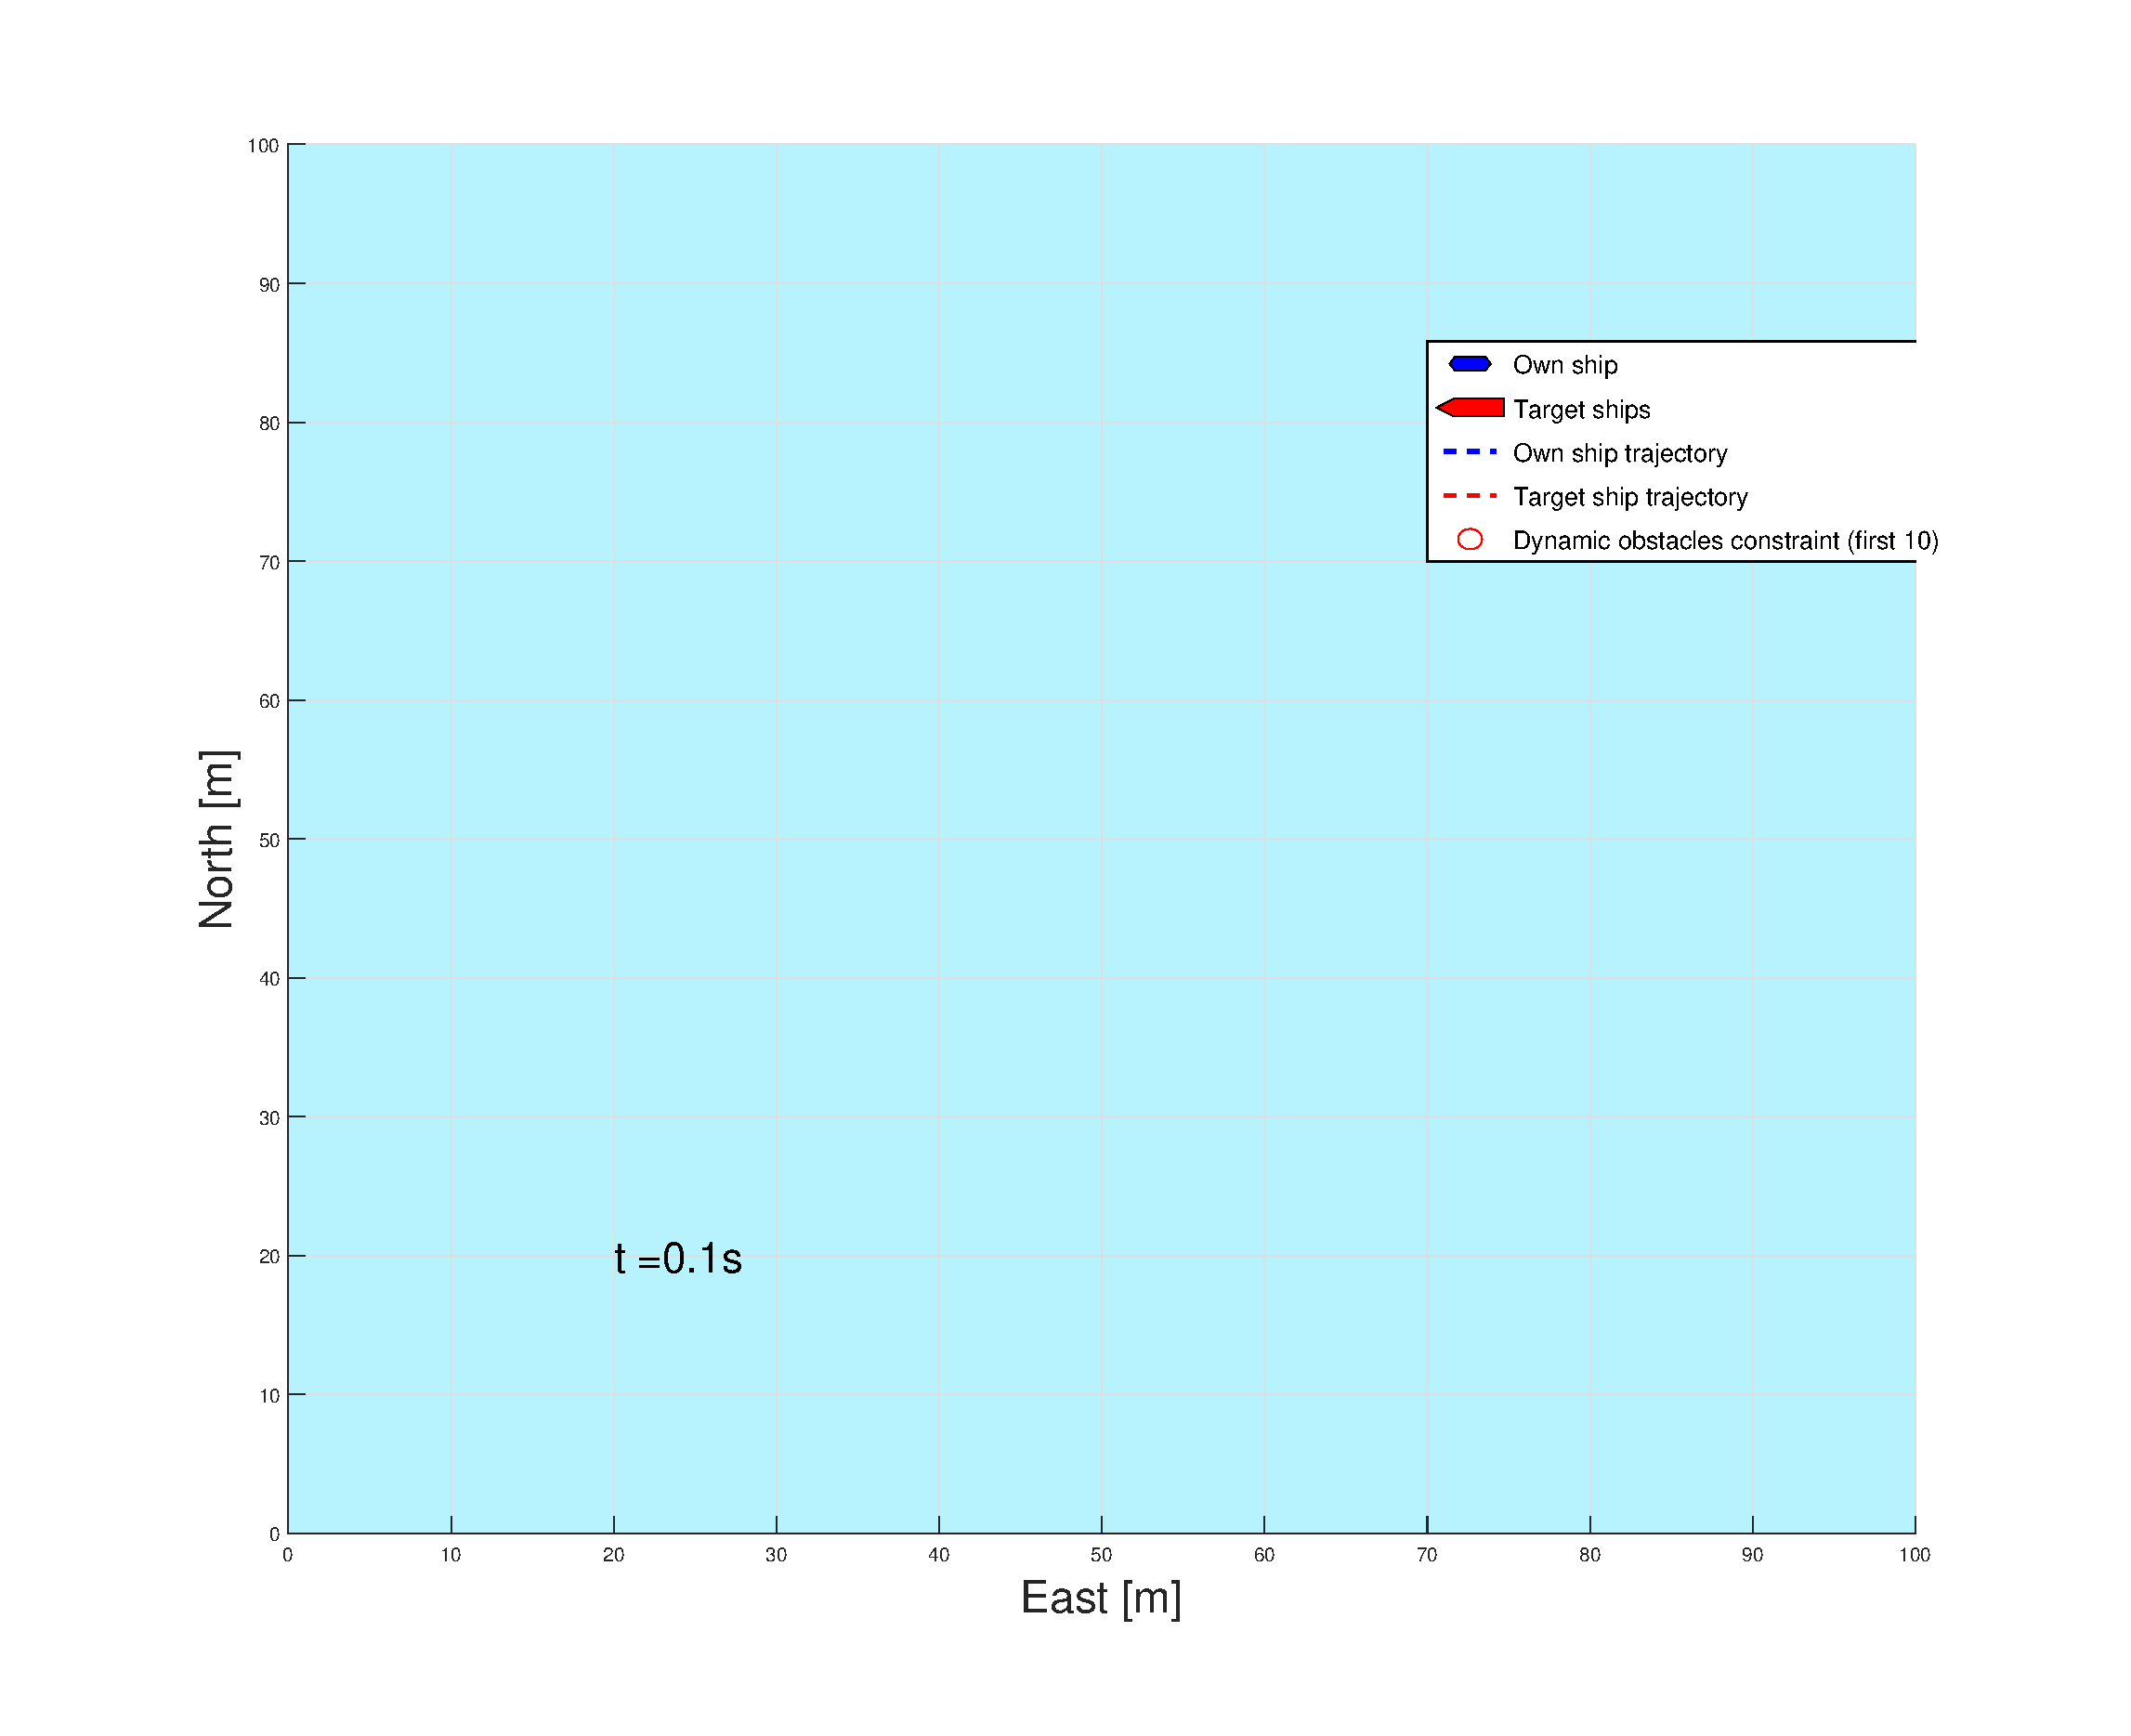
\includegraphics[width=\textwidth]{Images/Figures/enkel_GW/_Simple_1fig1_time=0}
        \subcaption{caption}
    \end{subfigure}
    \hfill
    \begin{subfigure}[b]{0.499\textwidth}
        \centering
        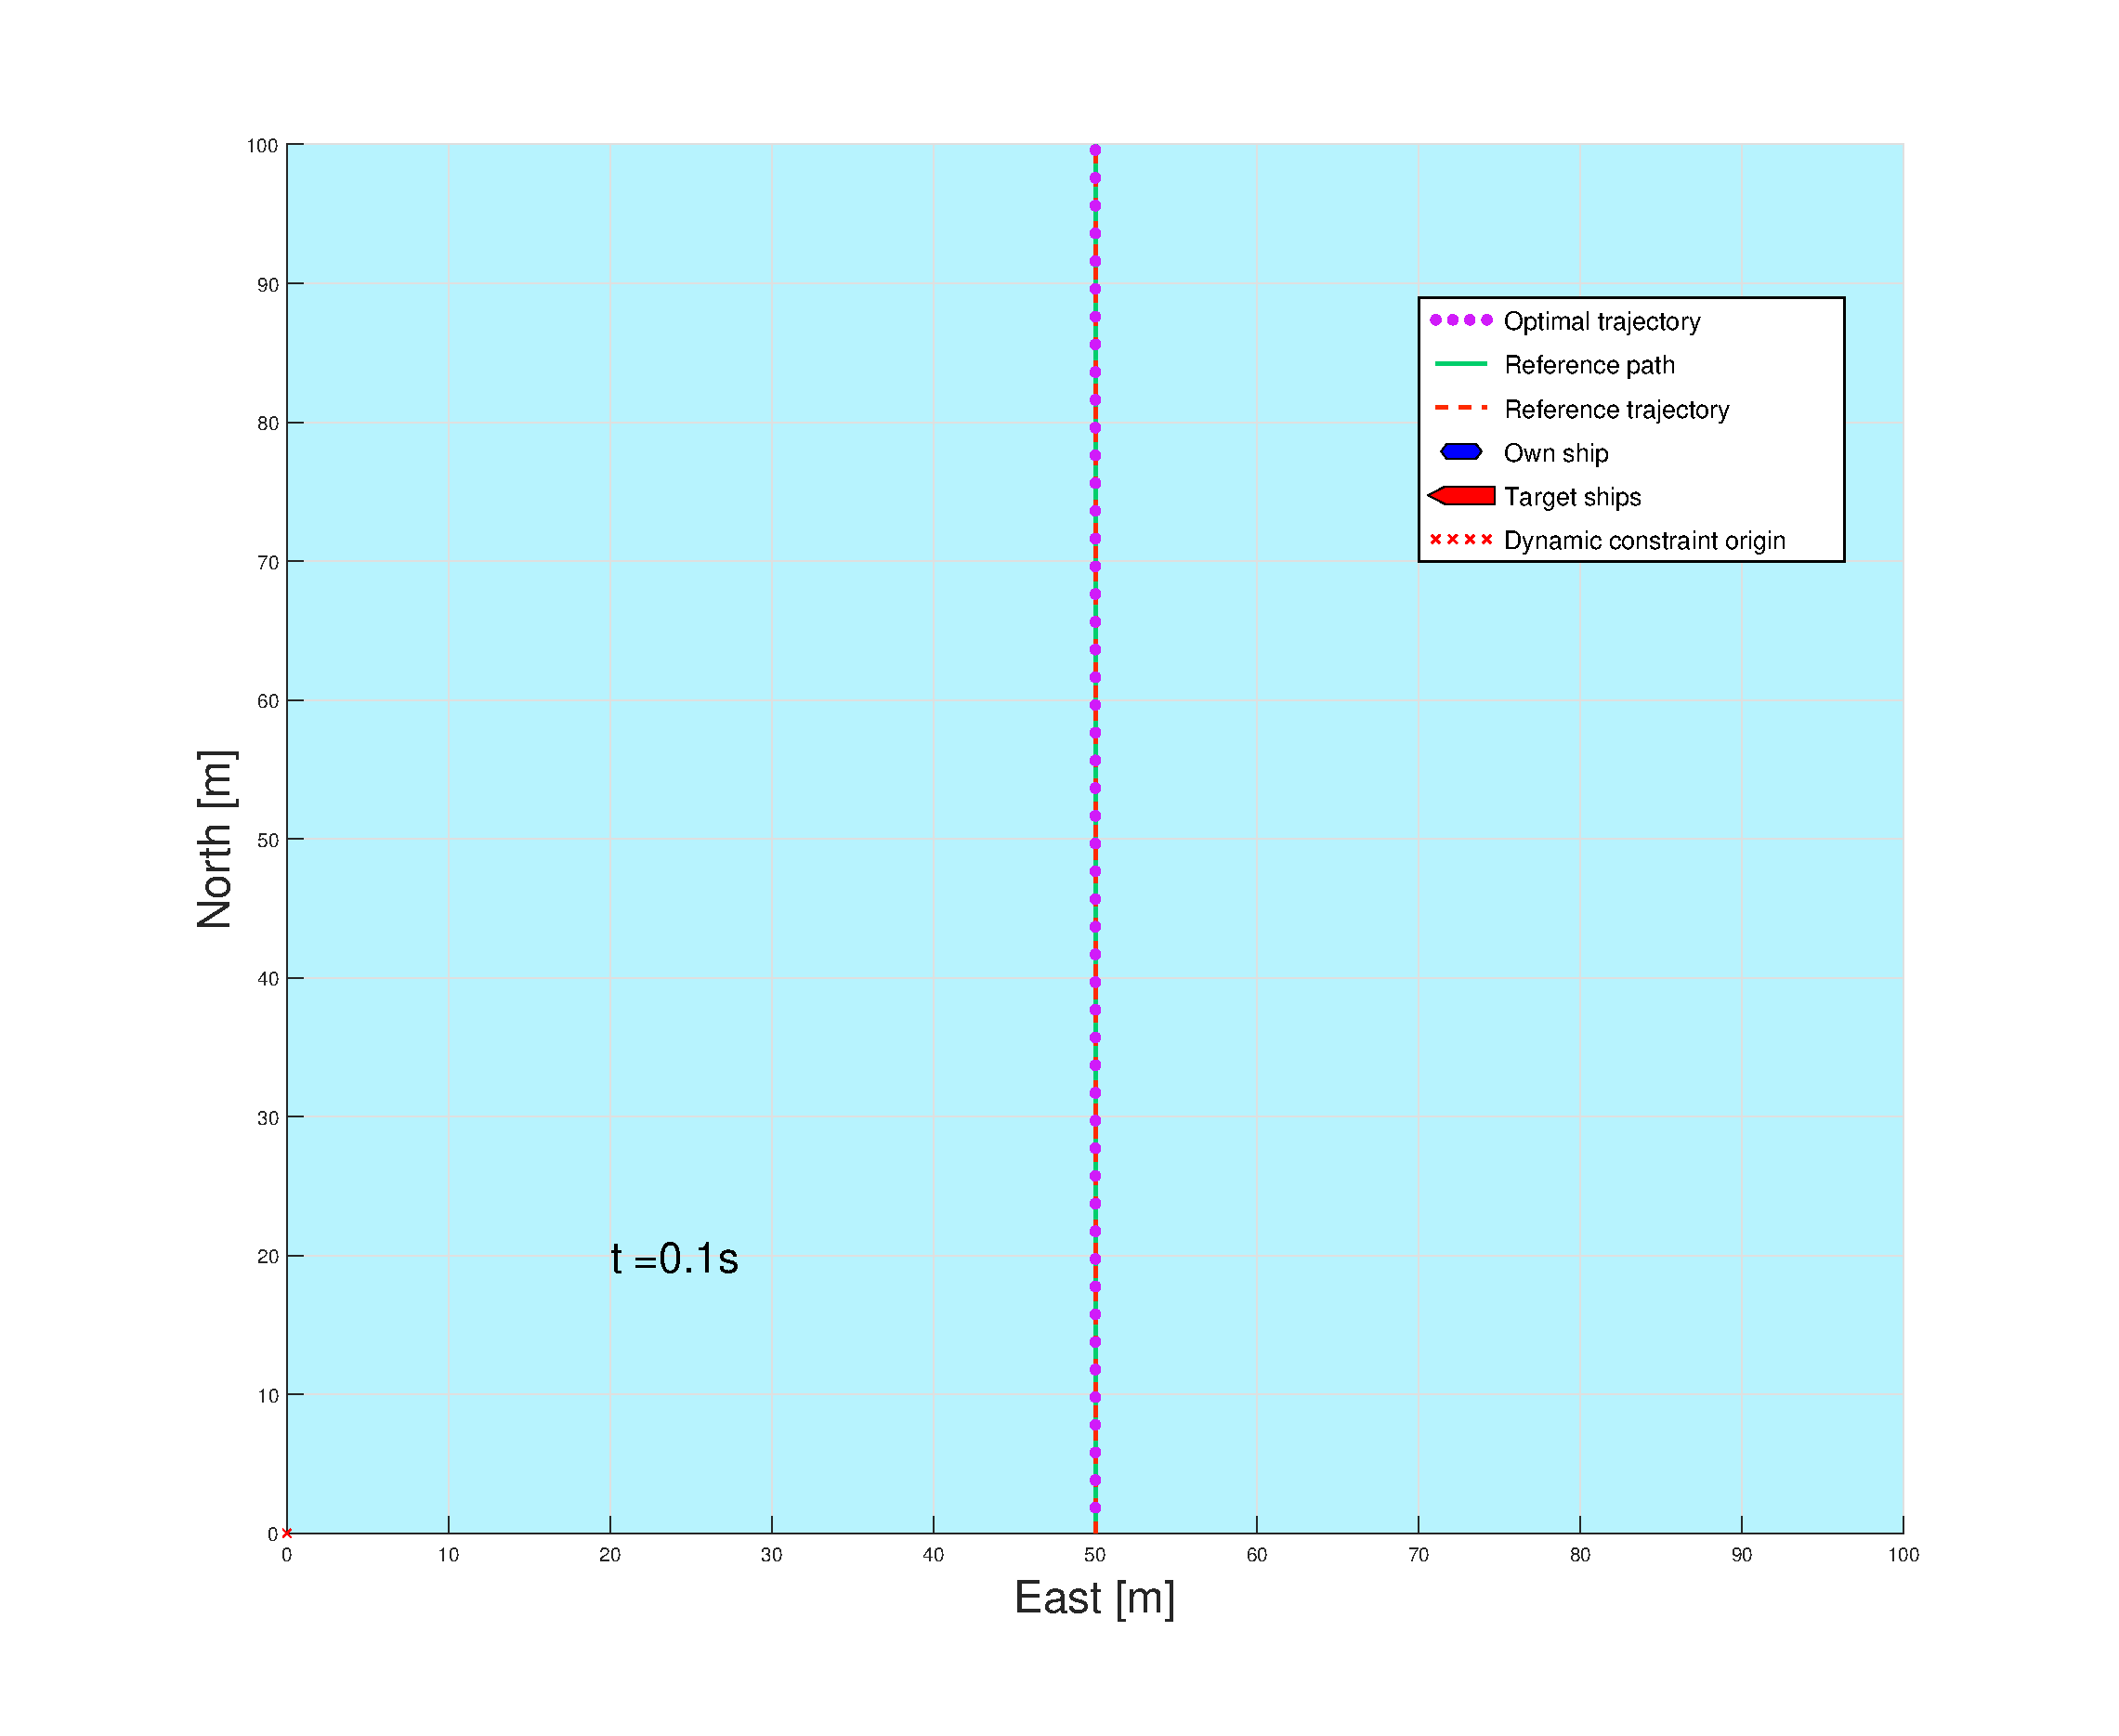
\includegraphics[width=\textwidth]{Images/Figures/enkel_GW/_Simple_1fig999_time=0}
        \subcaption{mhm}
    \end{subfigure}
    \hfill
    \\
    \begin{subfigure}[b]{0.49\textwidth}
        \centering
        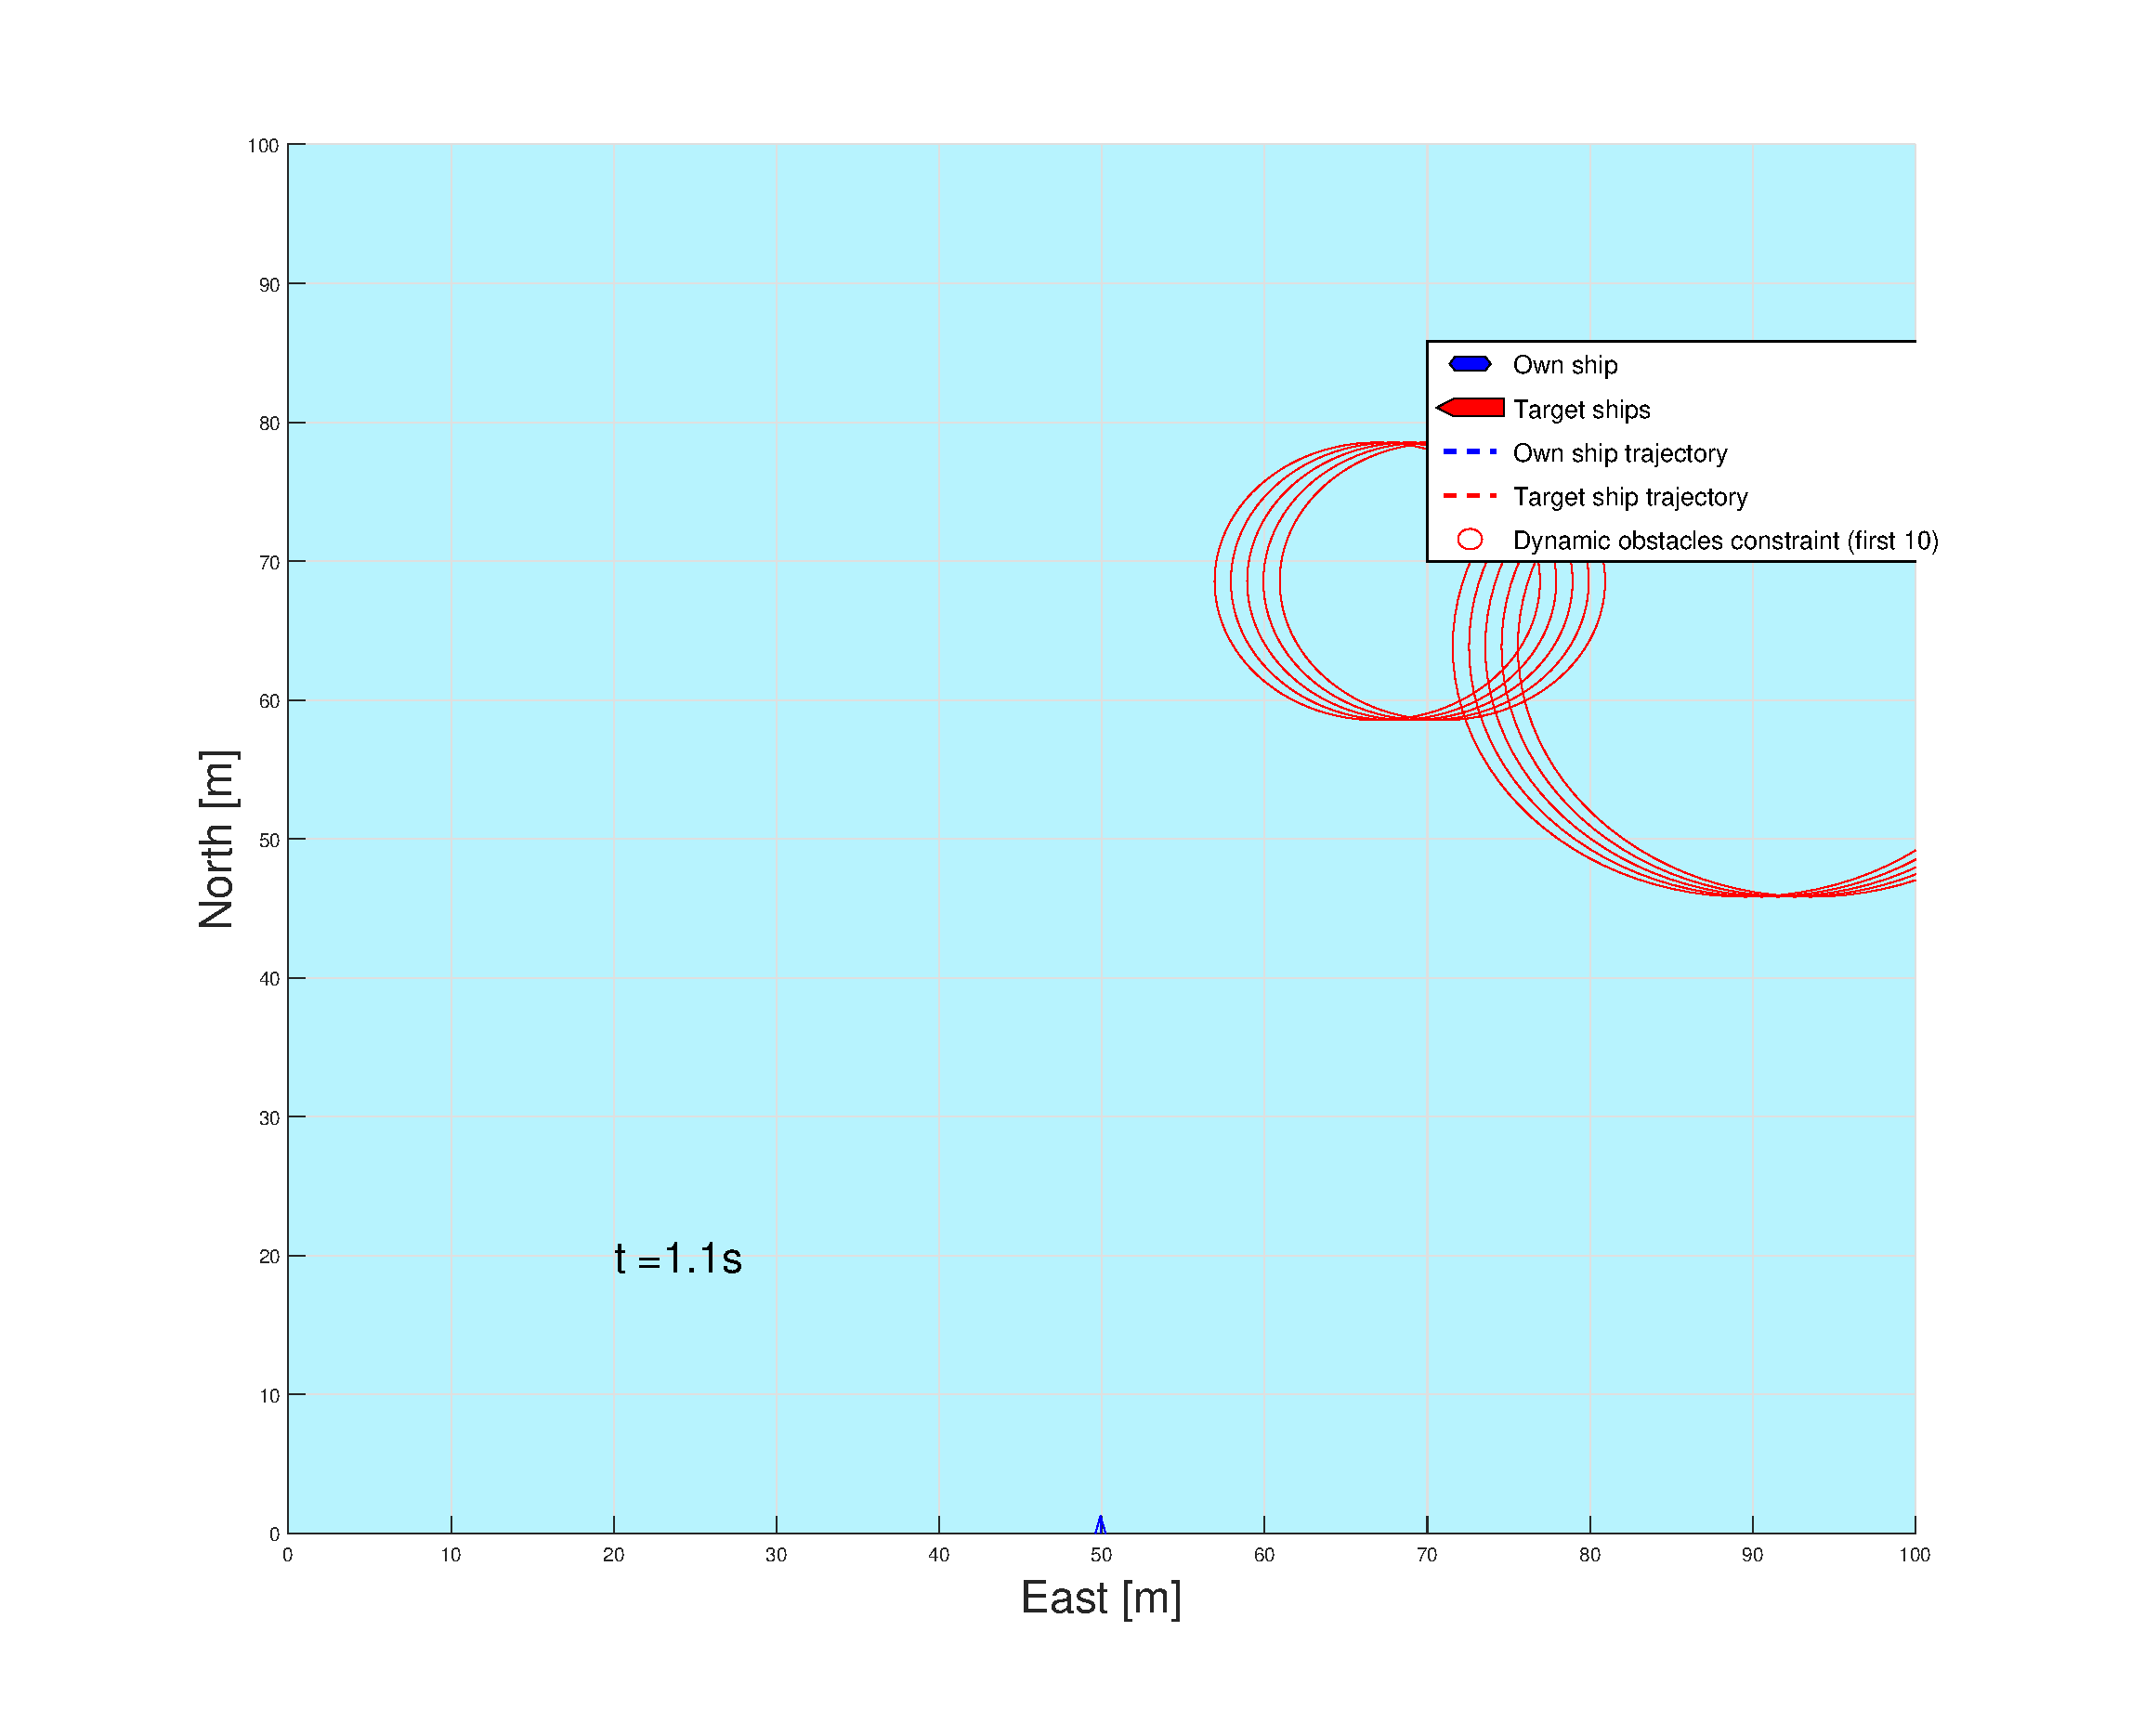
\includegraphics[width=\textwidth]{Images/Figures/enkel_GW/_Simple_1fig1_time=1}
        \subcaption{caption}
    \end{subfigure}
    \hfill
    \begin{subfigure}[b]{0.499\textwidth}
        \centering
        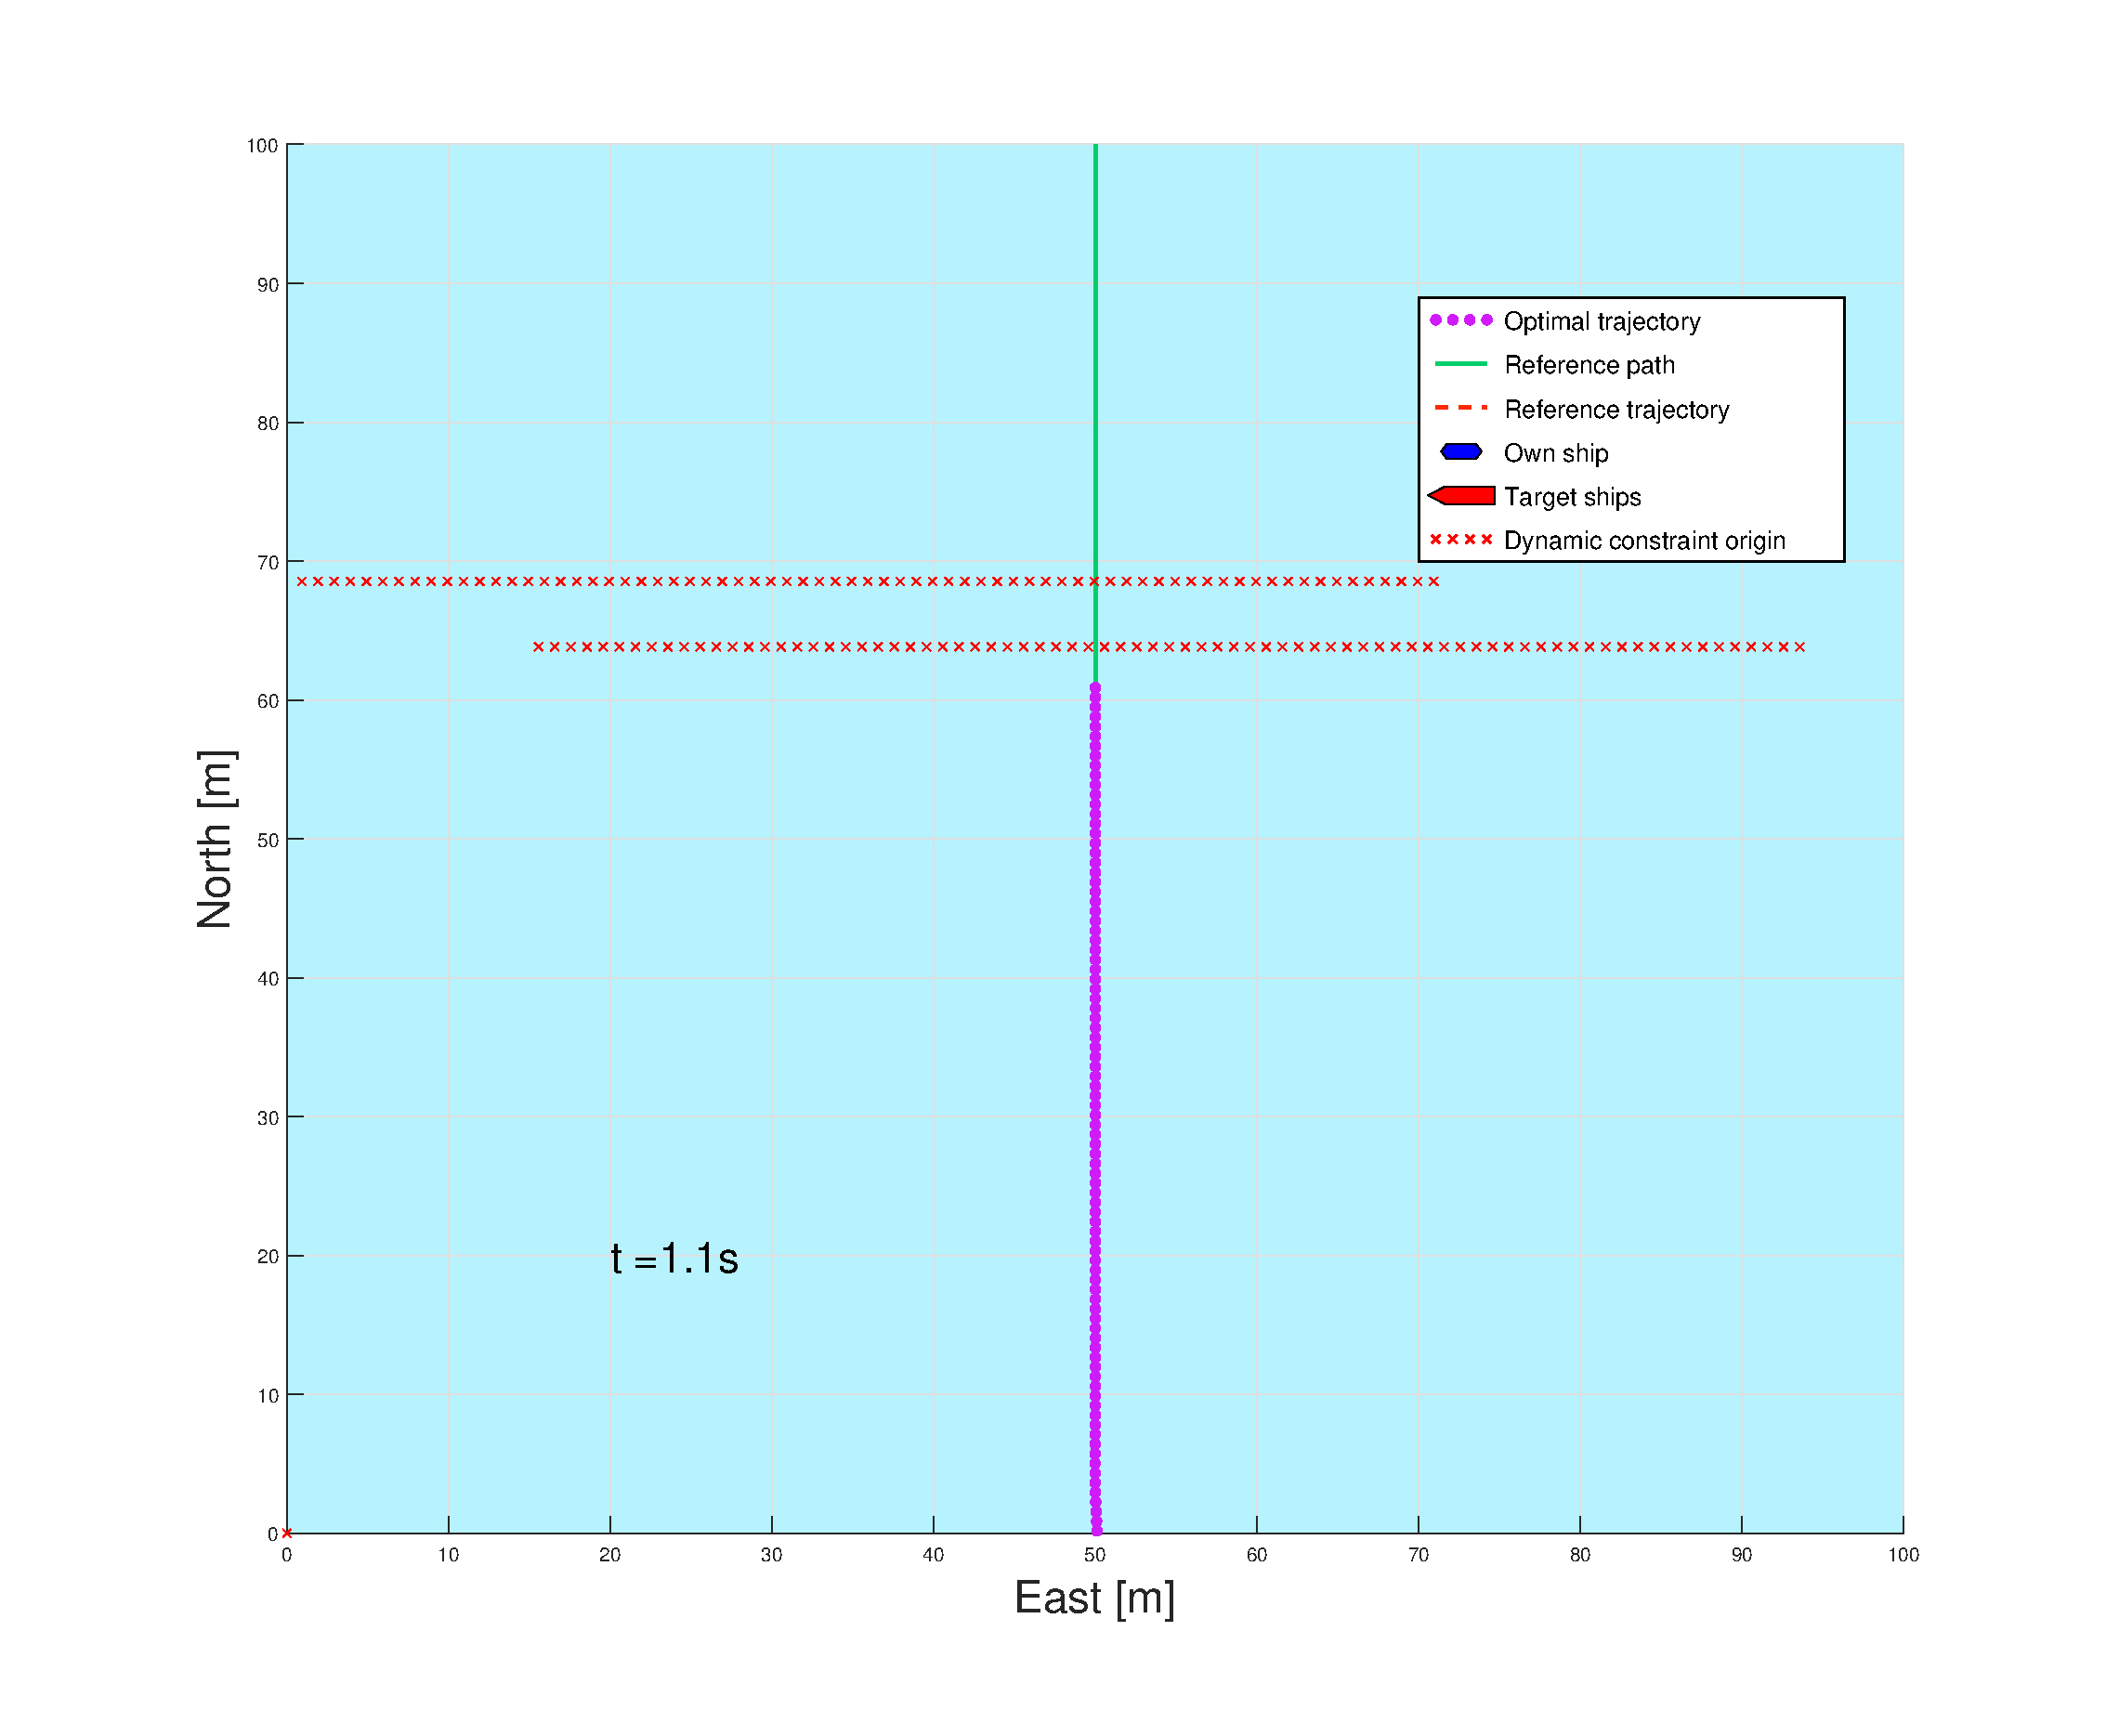
\includegraphics[width=\textwidth]{Images/Figures/enkel_GW/_Simple_1fig999_time=1}
        \subcaption{mhm}
    \end{subfigure}
    \hfill
    \\
    \begin{subfigure}[b]{0.49\textwidth}
        \centering
        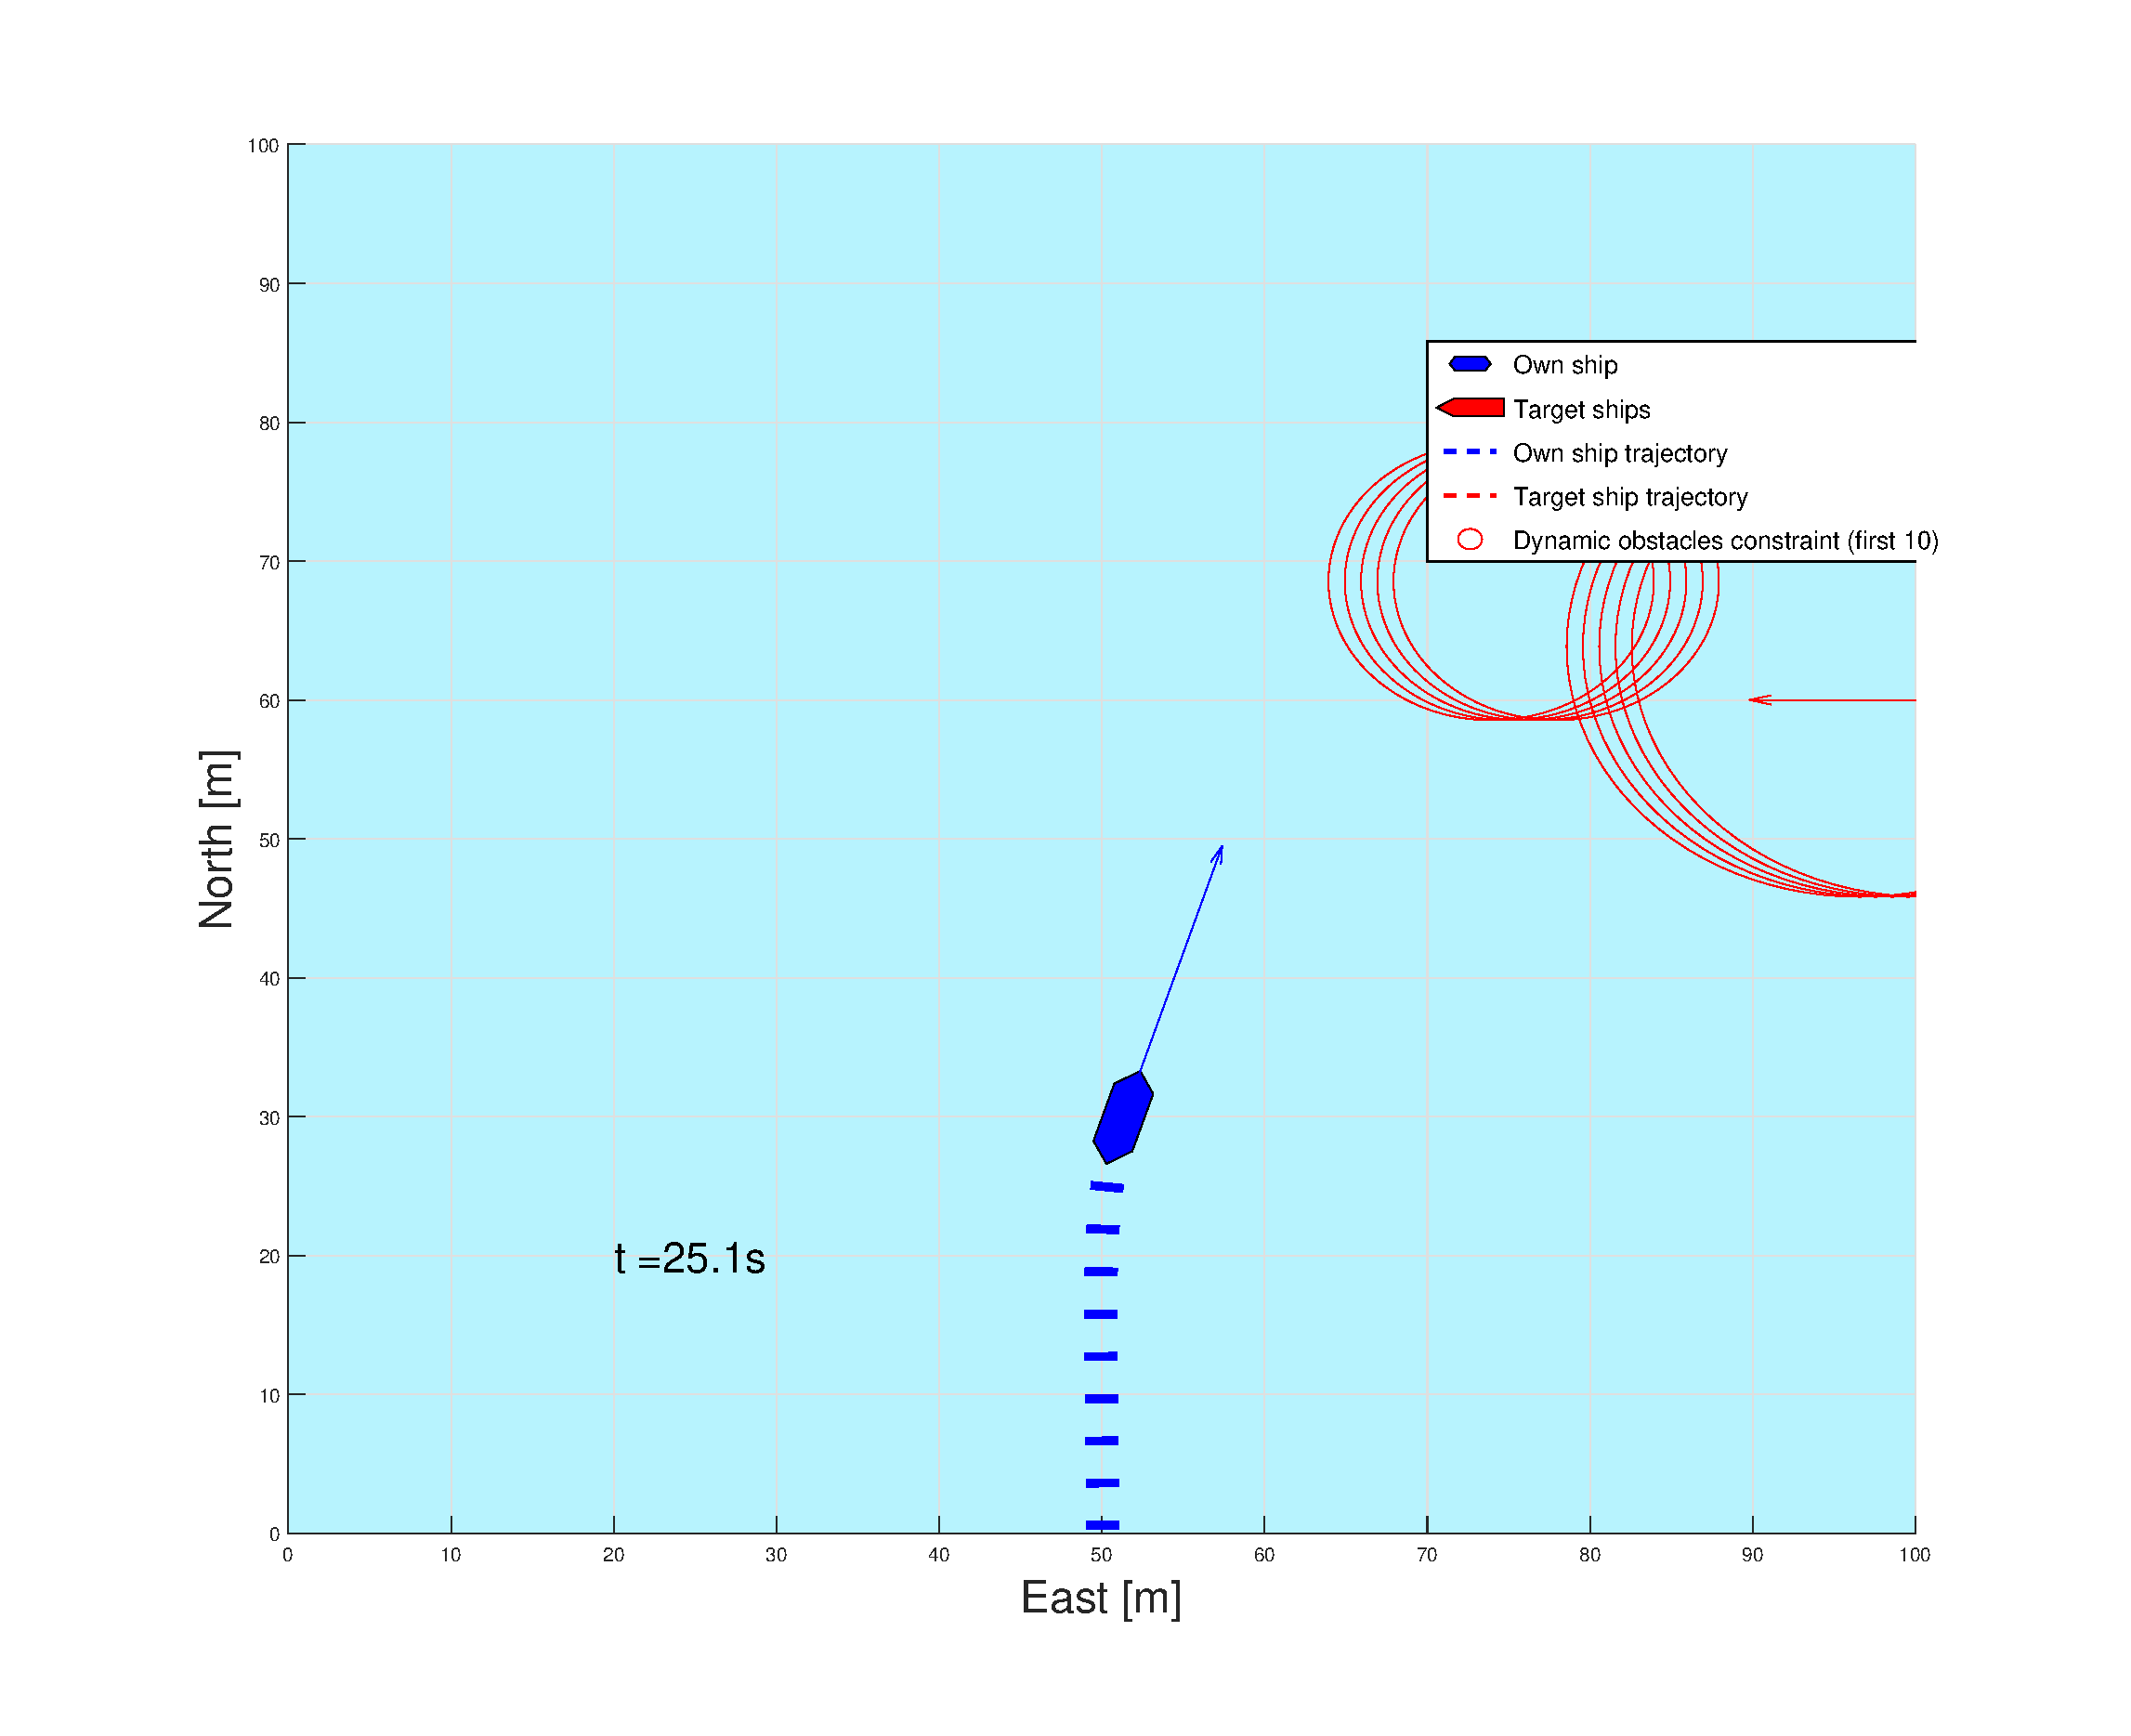
\includegraphics[width=\textwidth]{Images/Figures/enkel_GW/_Simple_1fig1_time=25}
        \subcaption{caption}
    \end{subfigure}
    \hfill
    \begin{subfigure}[b]{0.499\textwidth}
        \centering
        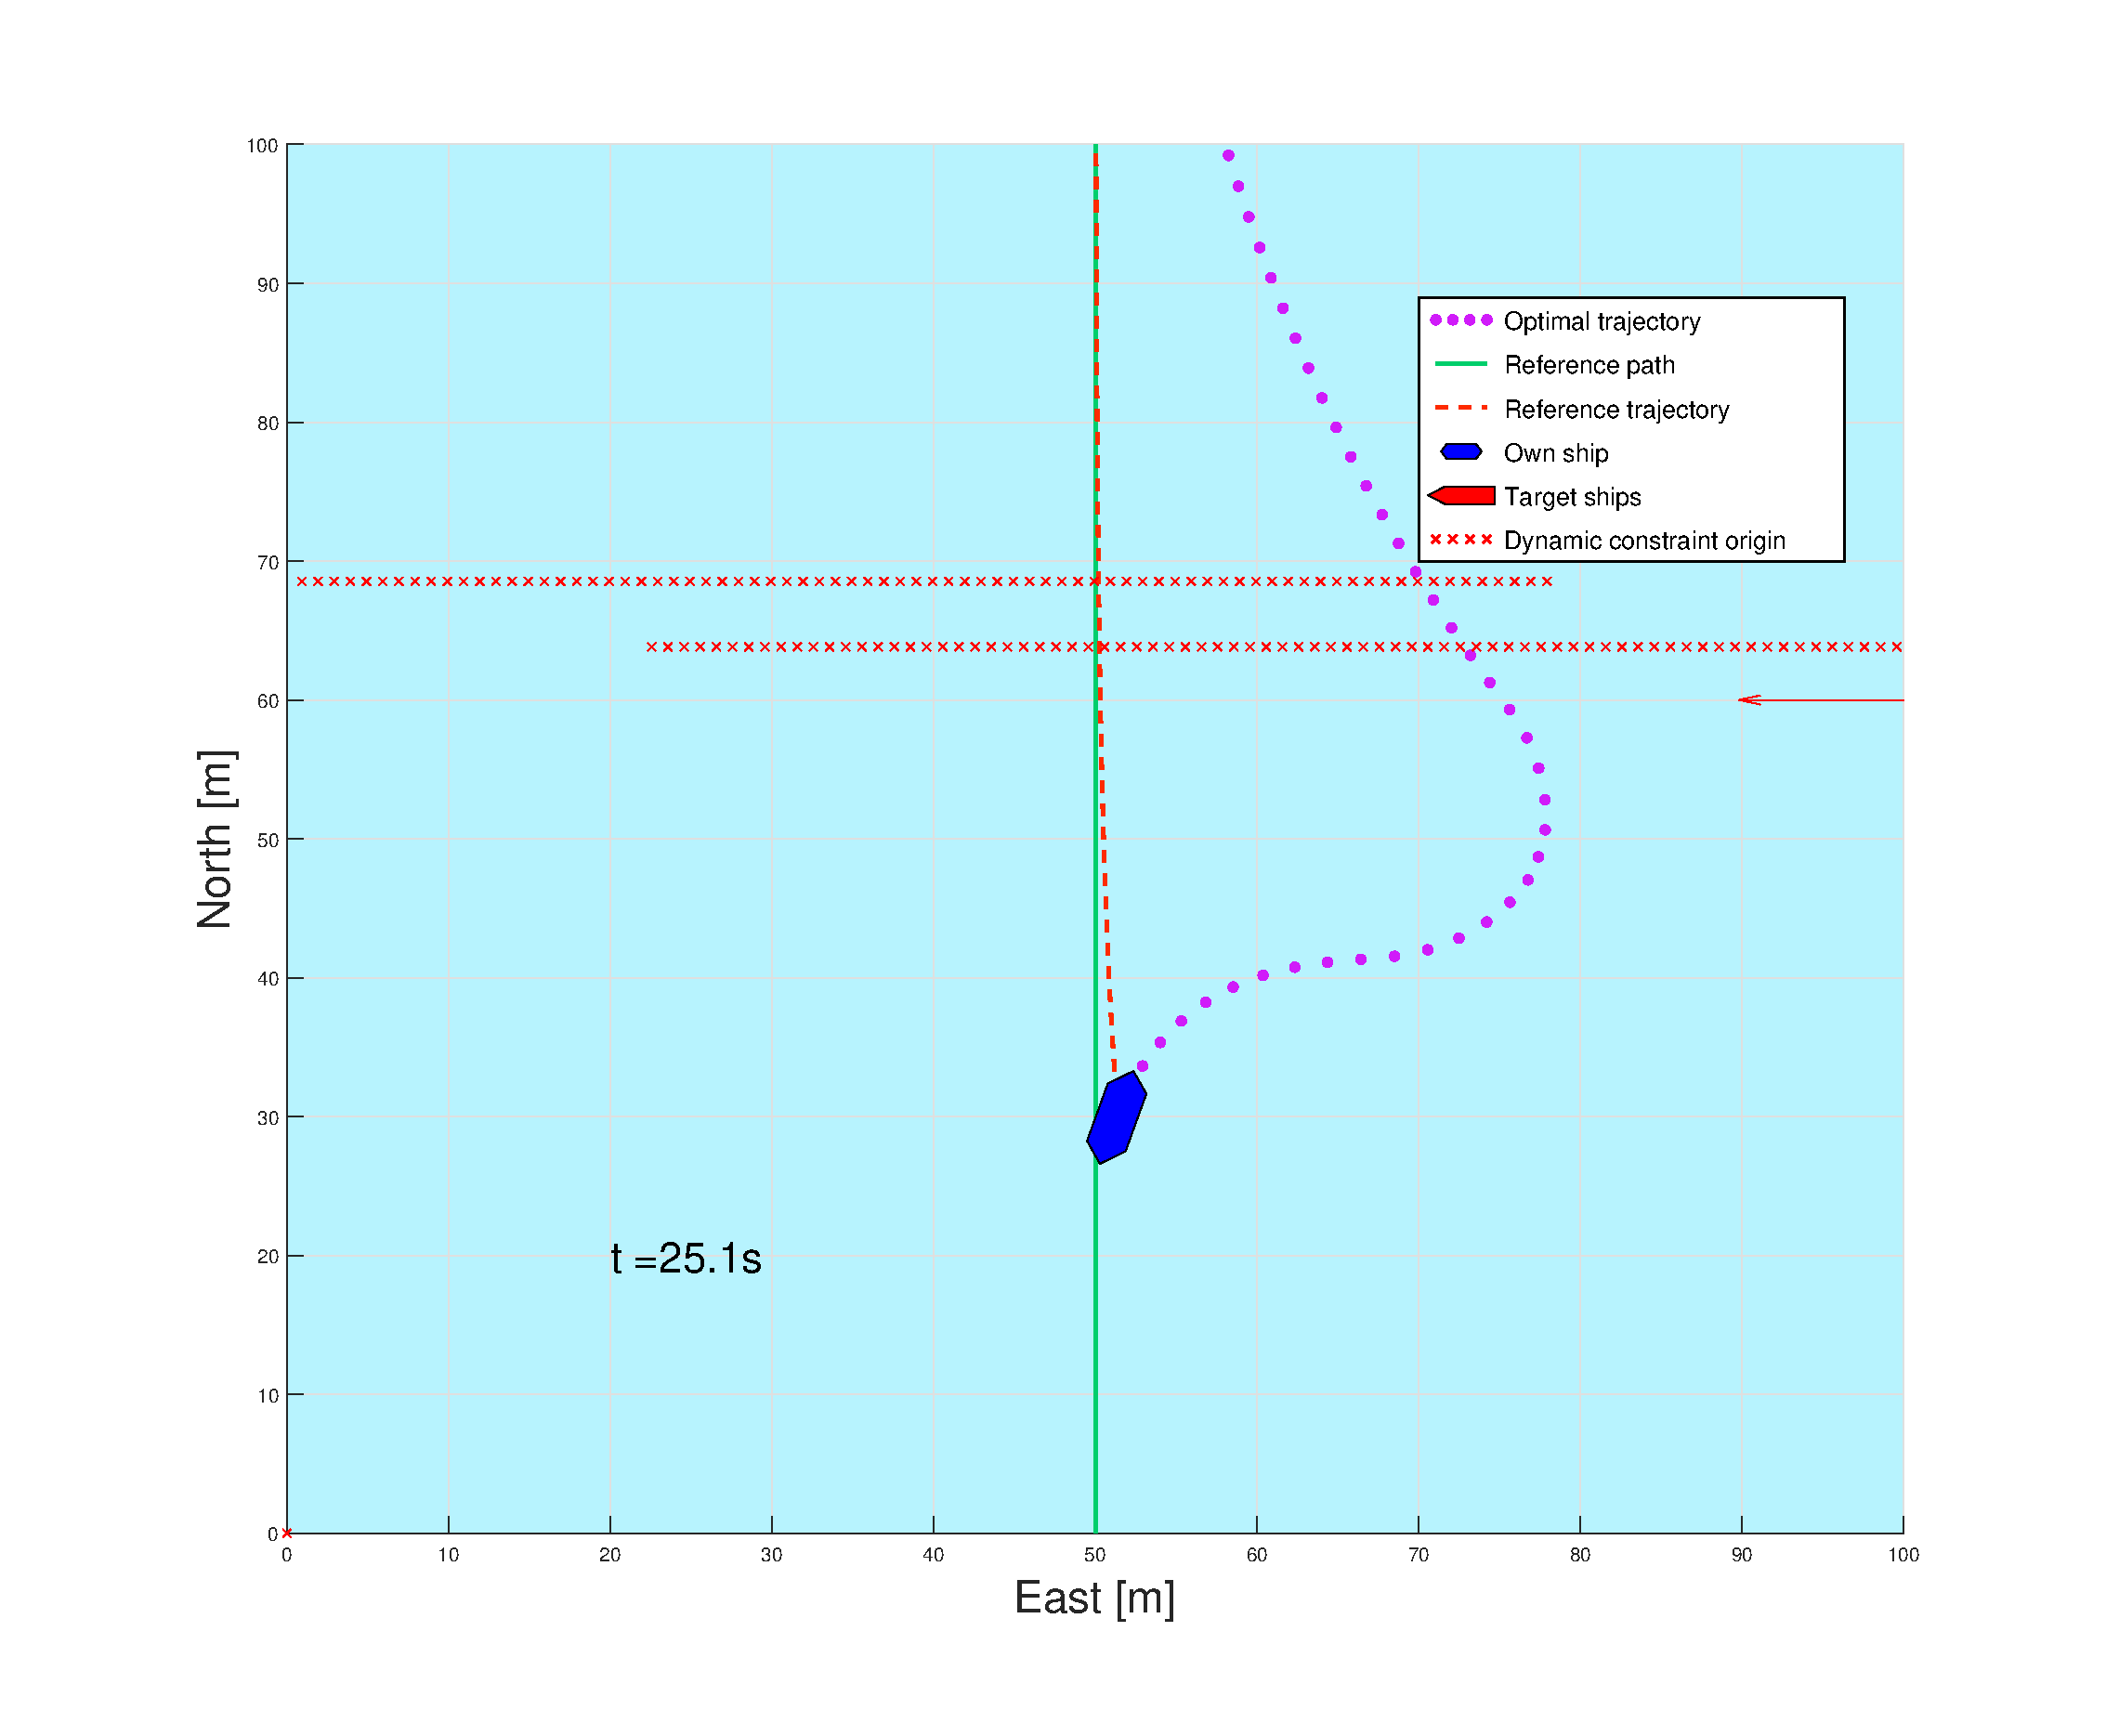
\includegraphics[width=\textwidth]{Images/Figures/enkel_GW/_Simple_1fig999_time=25}
        \subcaption{mhm}
    \end{subfigure}
    \hfill
\end{figure}%
\begin{figure}[ht]\ContinuedFloat
    \begin{subfigure}[b]{0.49\textwidth}
        \centering
        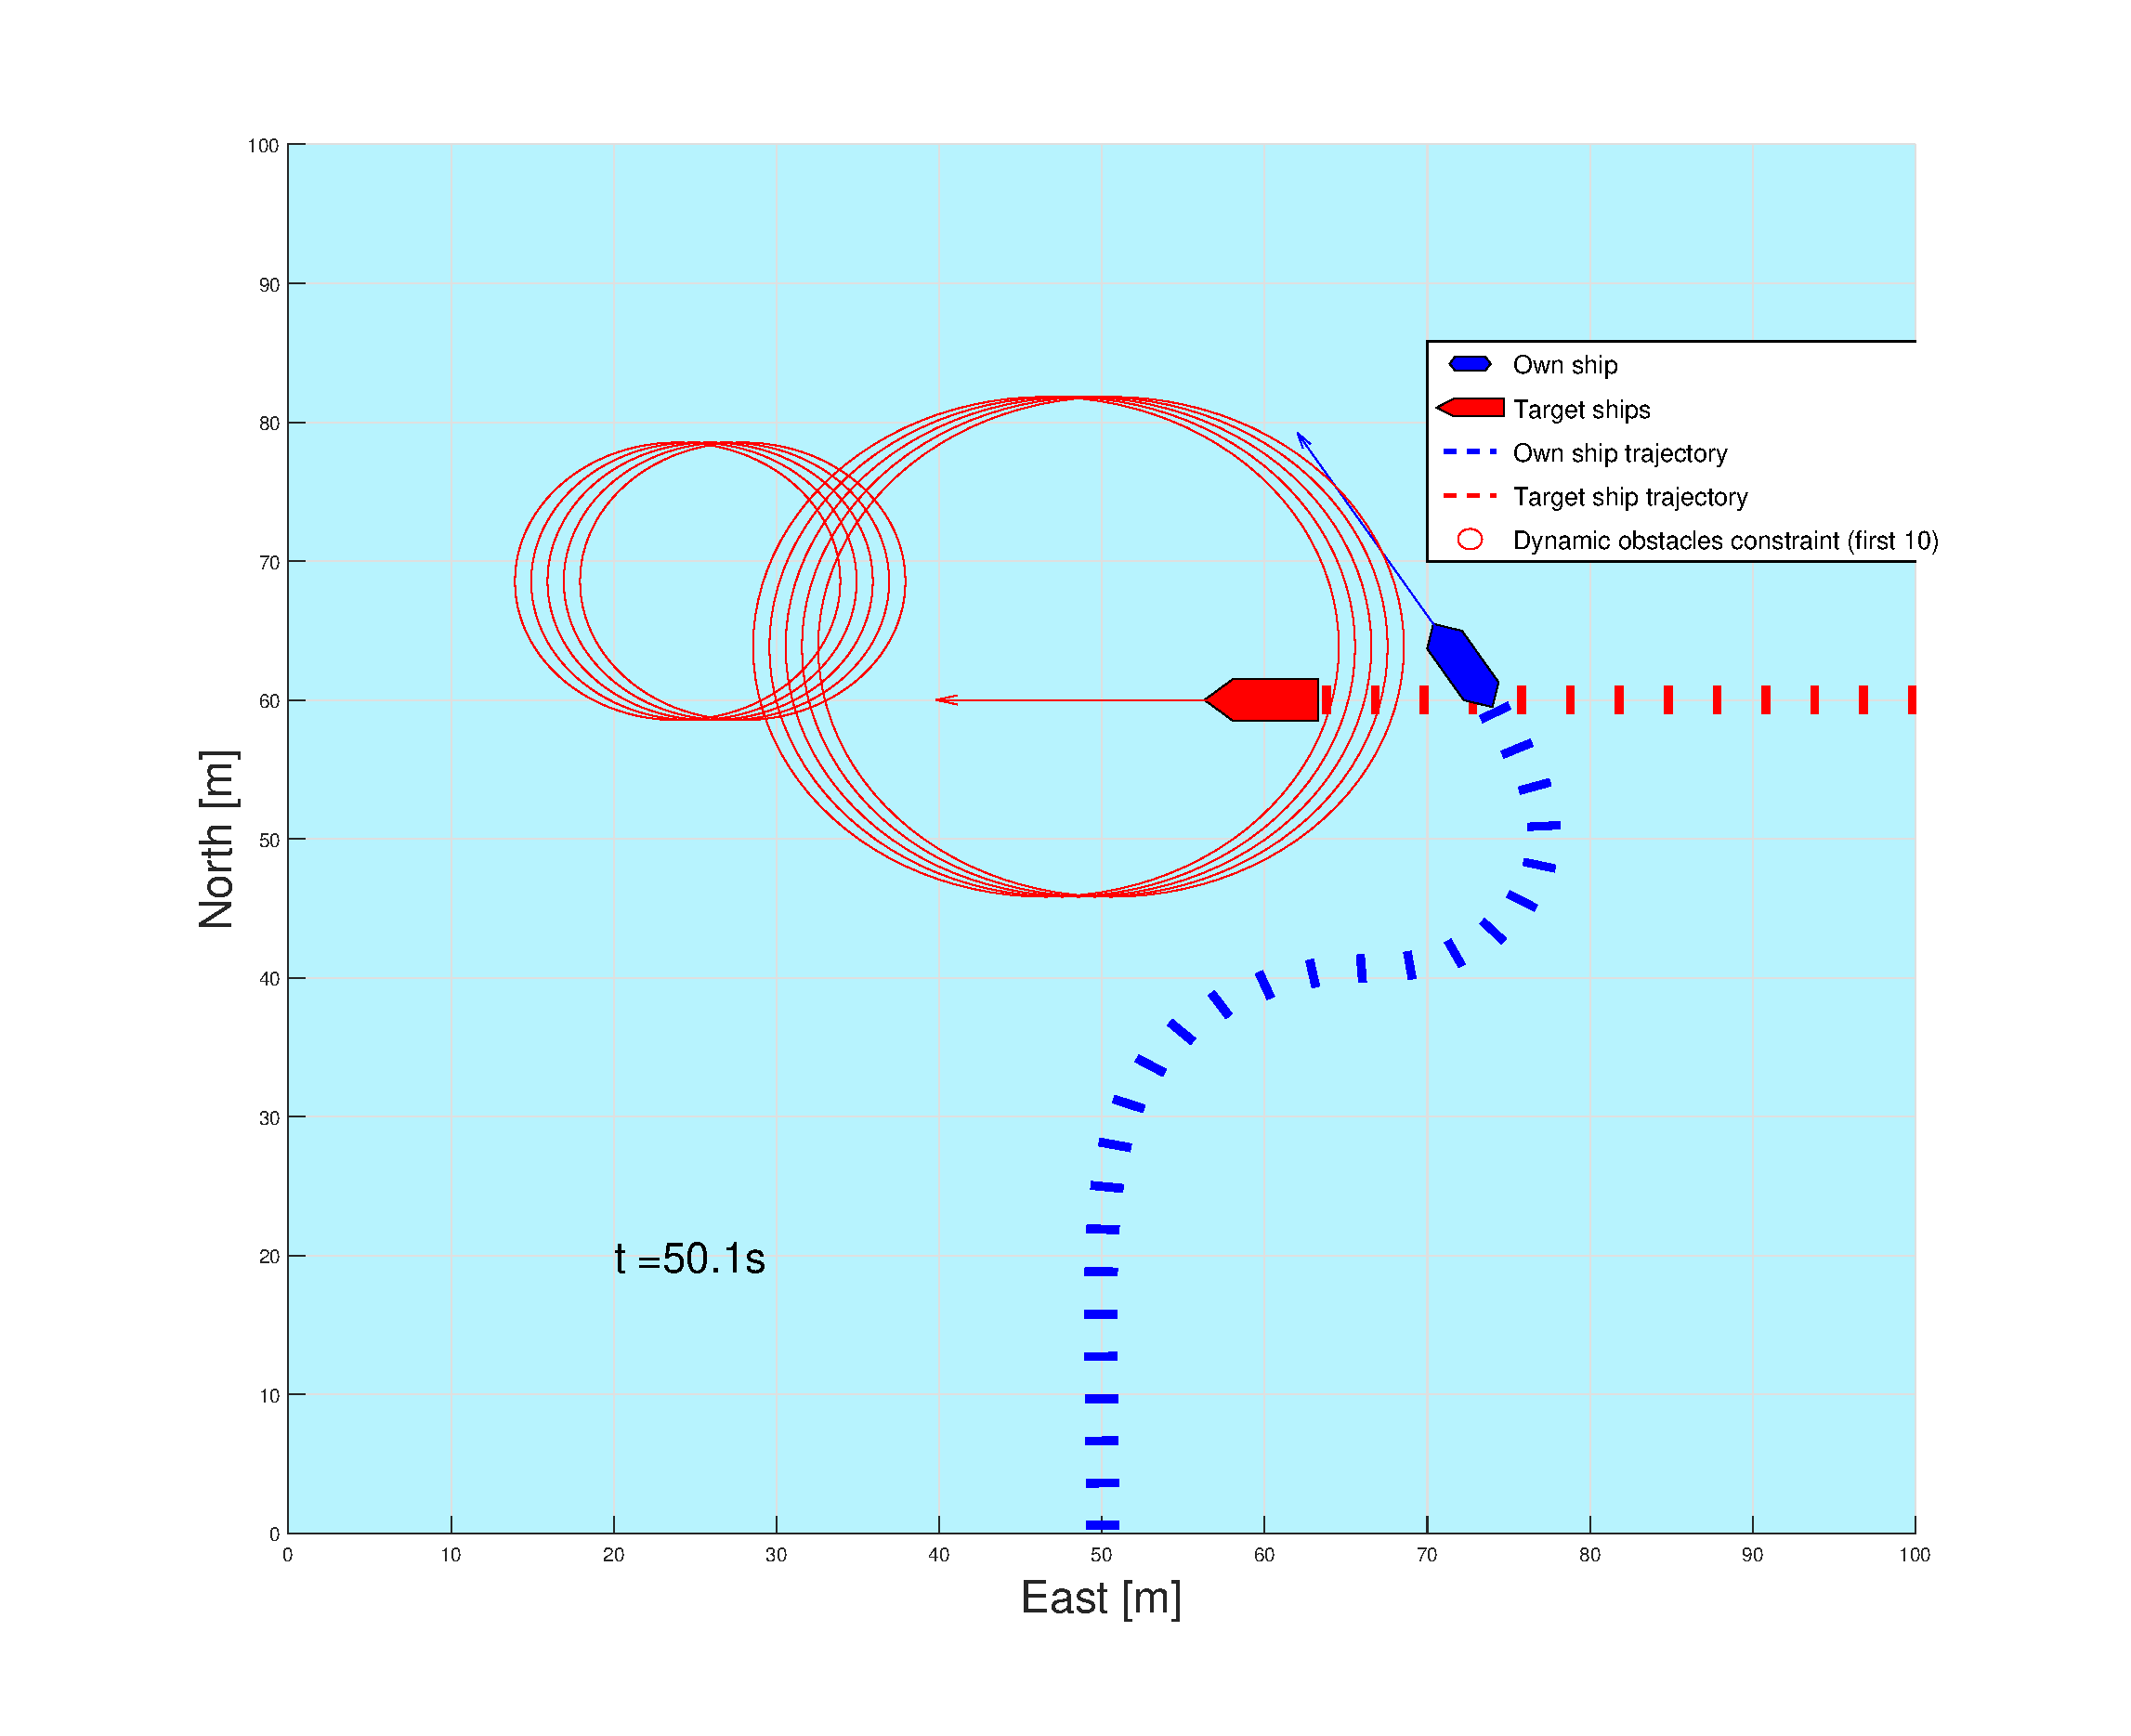
\includegraphics[width=\textwidth]{Images/Figures/enkel_GW/_Simple_1fig1_time=50}
        \subcaption{caption}
    \end{subfigure}
    \hfill
    \begin{subfigure}[b]{0.499\textwidth}
        \centering
        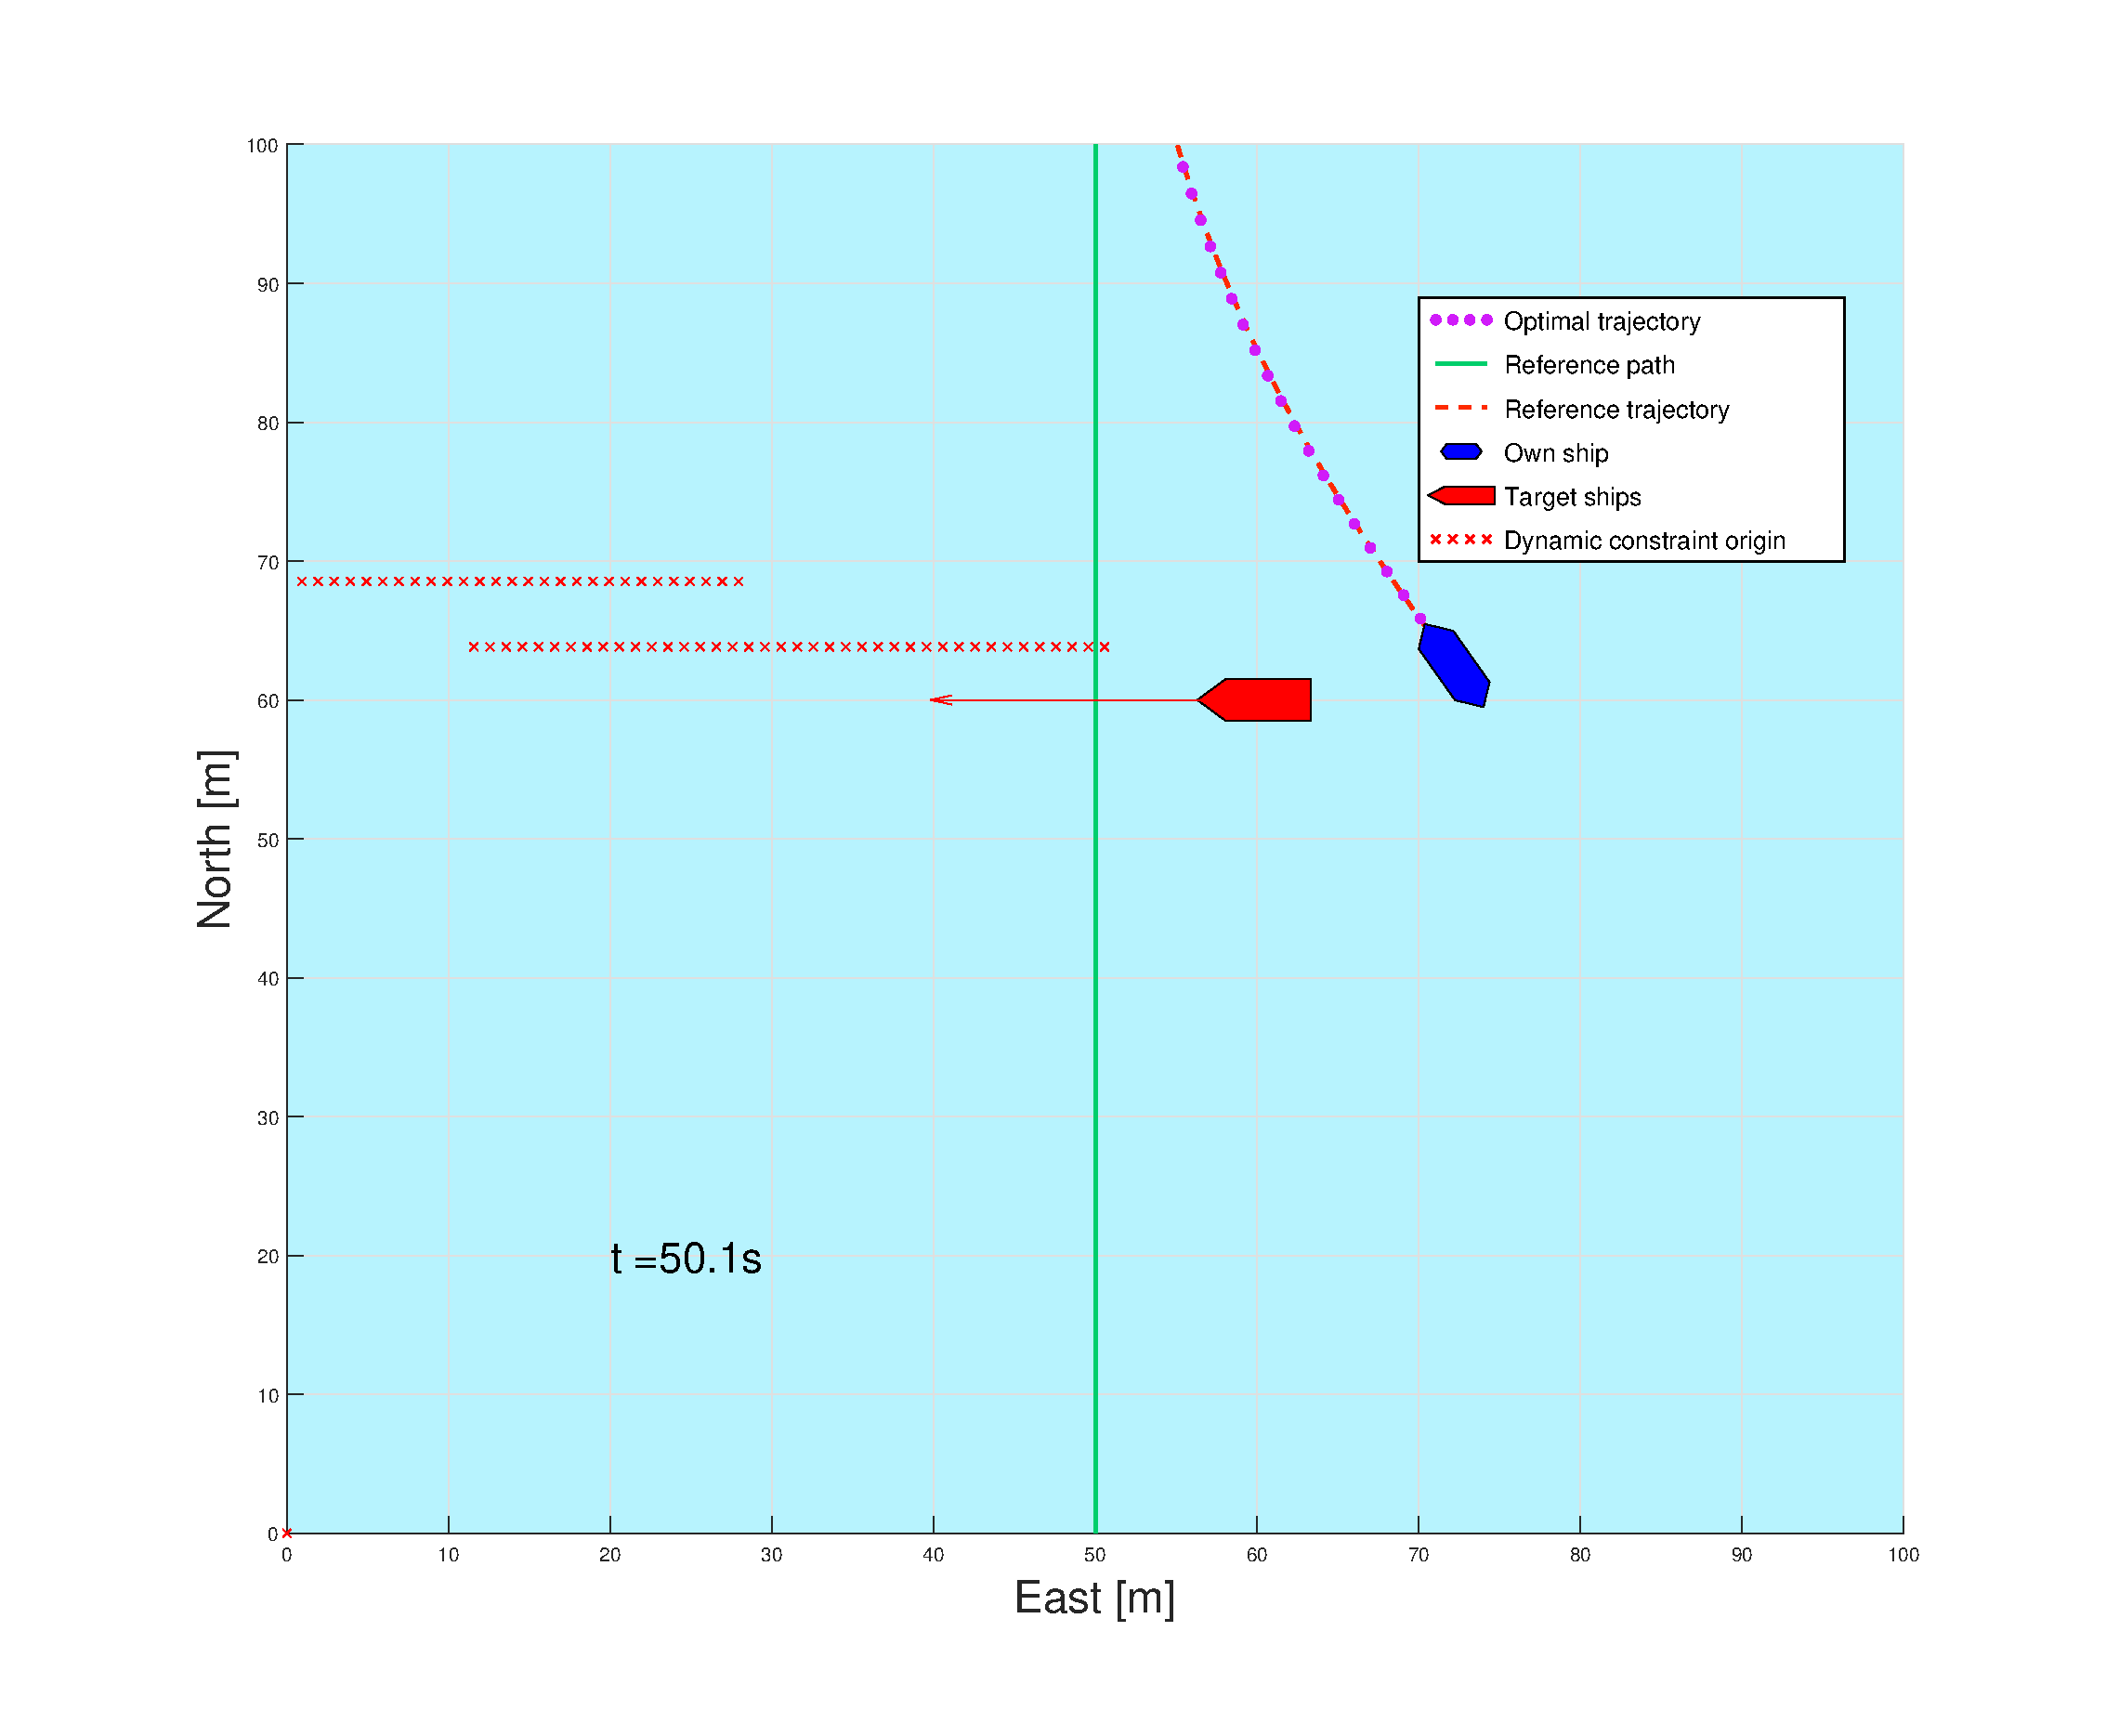
\includegraphics[width=\textwidth]{Images/Figures/enkel_GW/_Simple_1fig999_time=50}
        \subcaption{mhm}
    \end{subfigure}
    \hfill
    \\
    \begin{subfigure}[b]{0.49\textwidth}
        \centering
        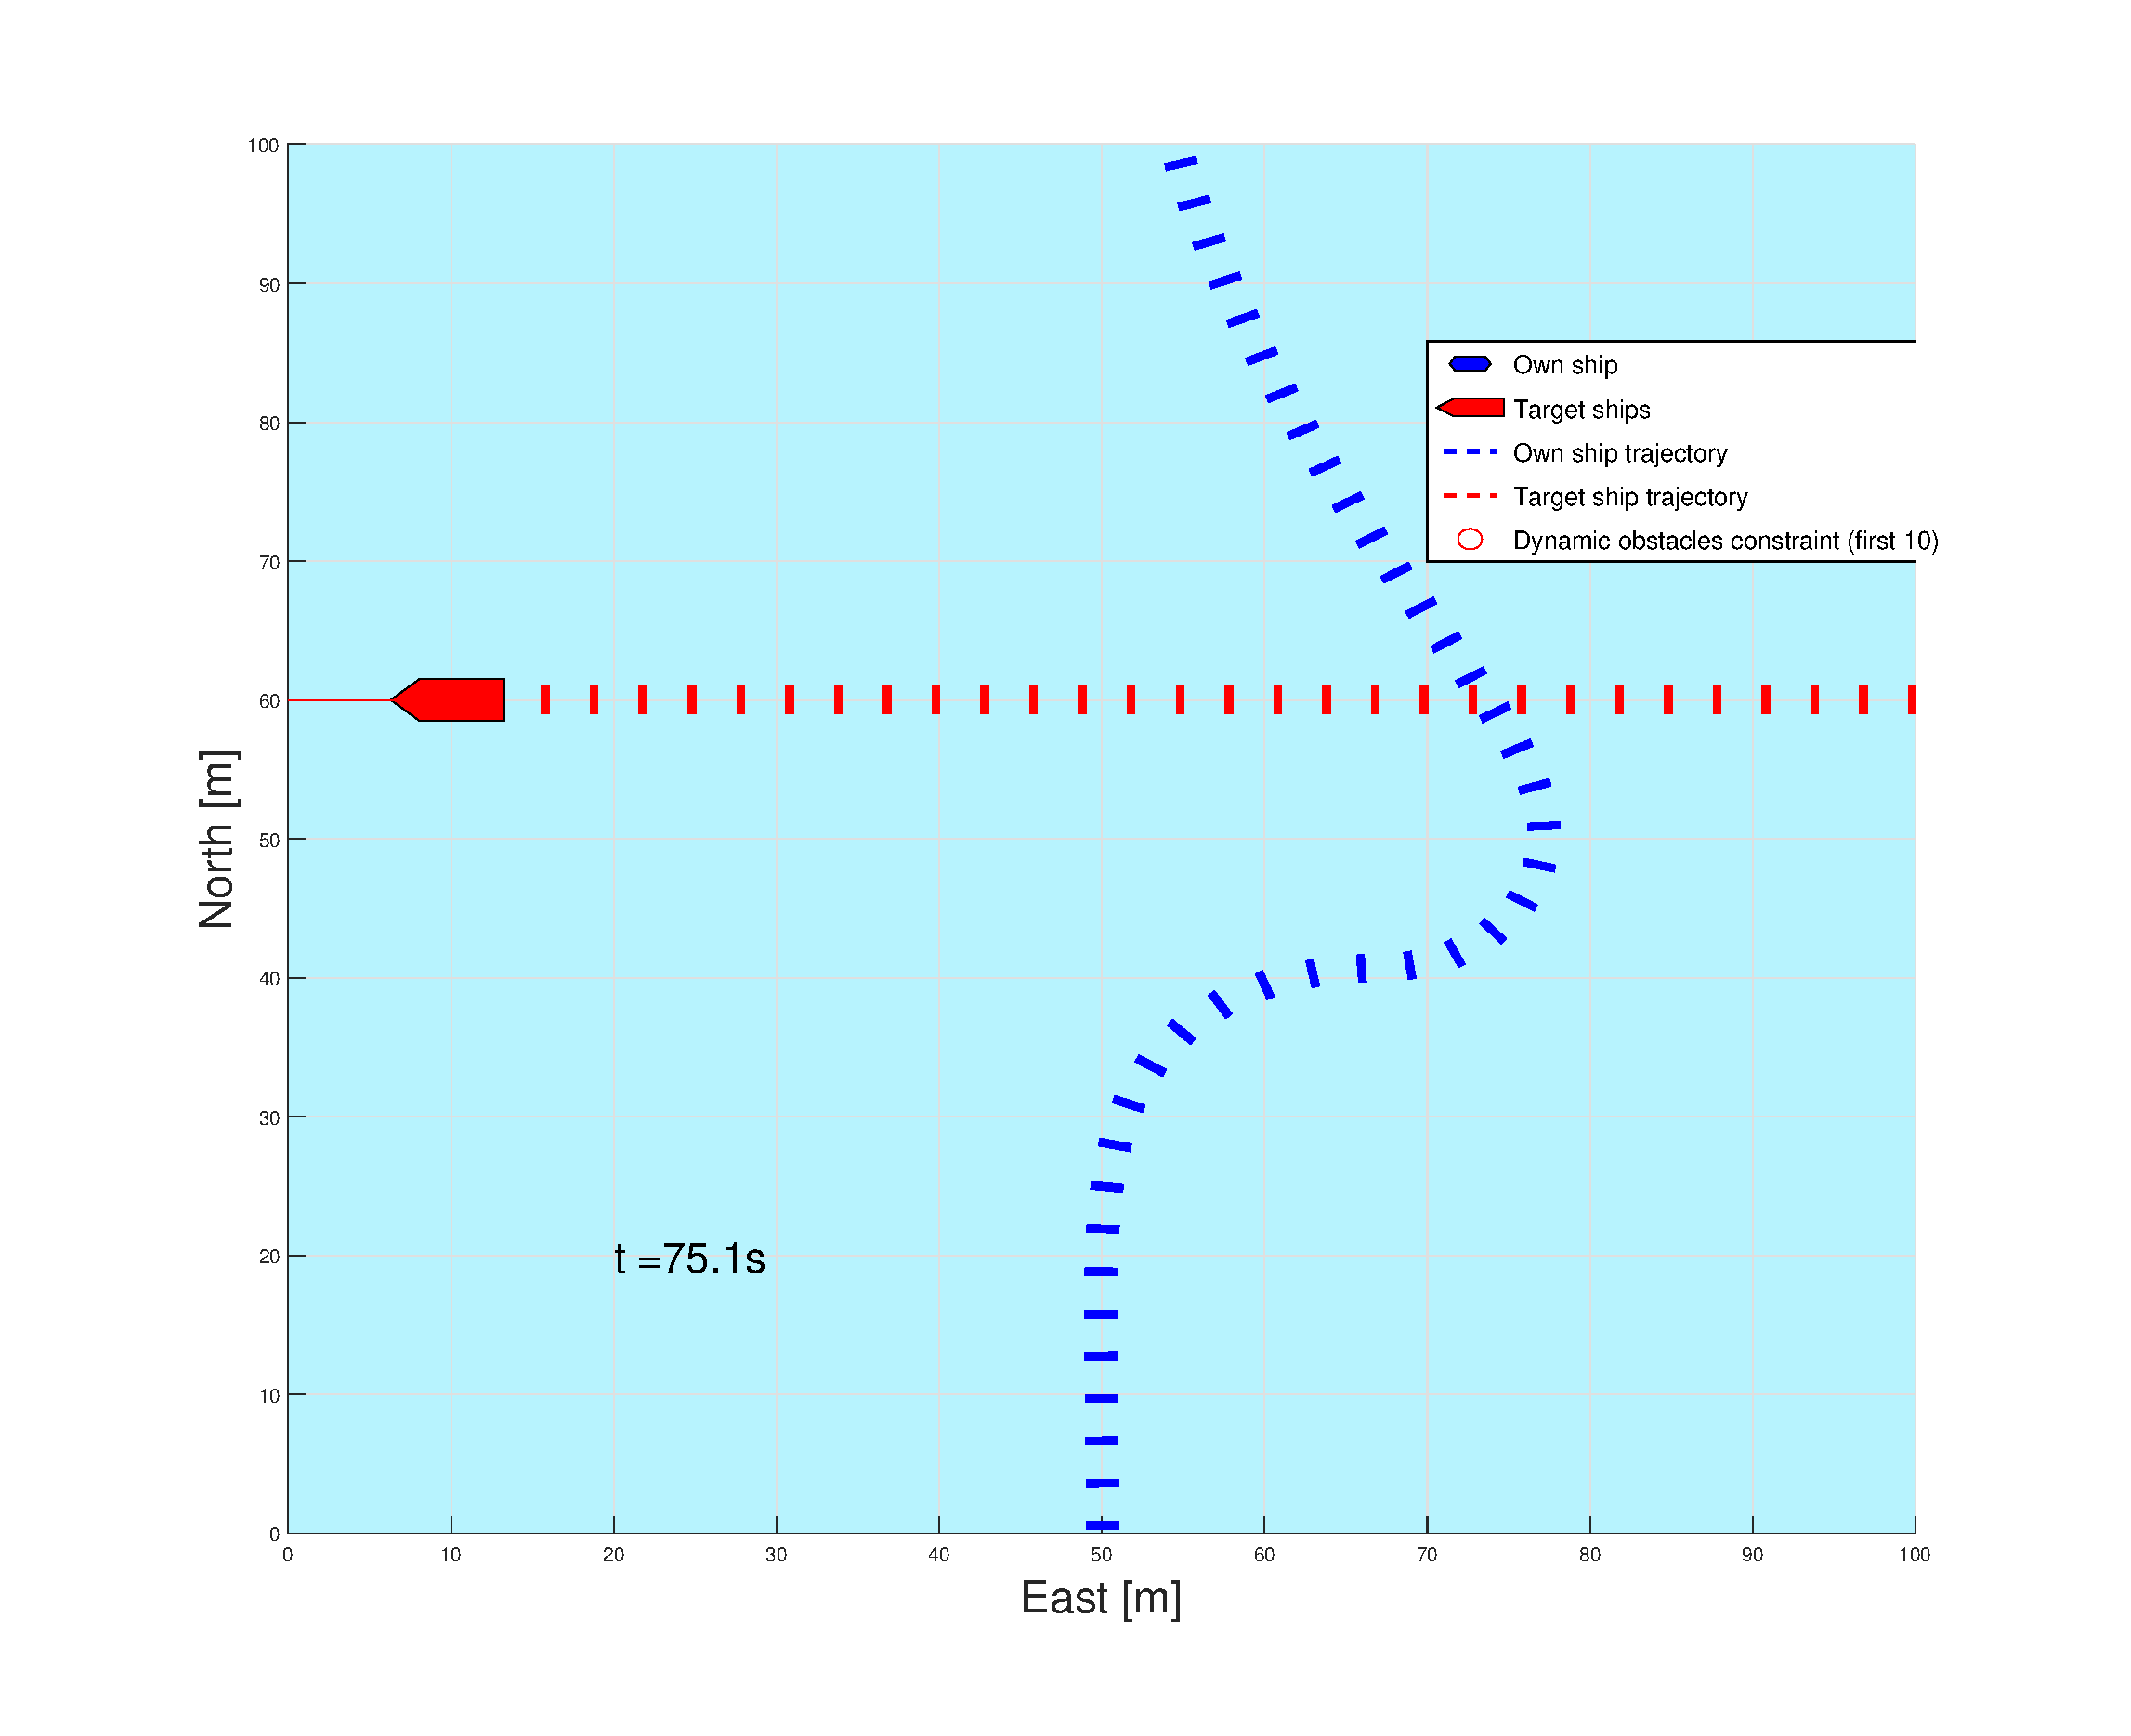
\includegraphics[width=\textwidth]{Images/Figures/enkel_GW/_Simple_1fig1_time=75}
        \subcaption{caption}
    \end{subfigure}
    \hfill
    \begin{subfigure}[b]{0.499\textwidth}
        \centering
        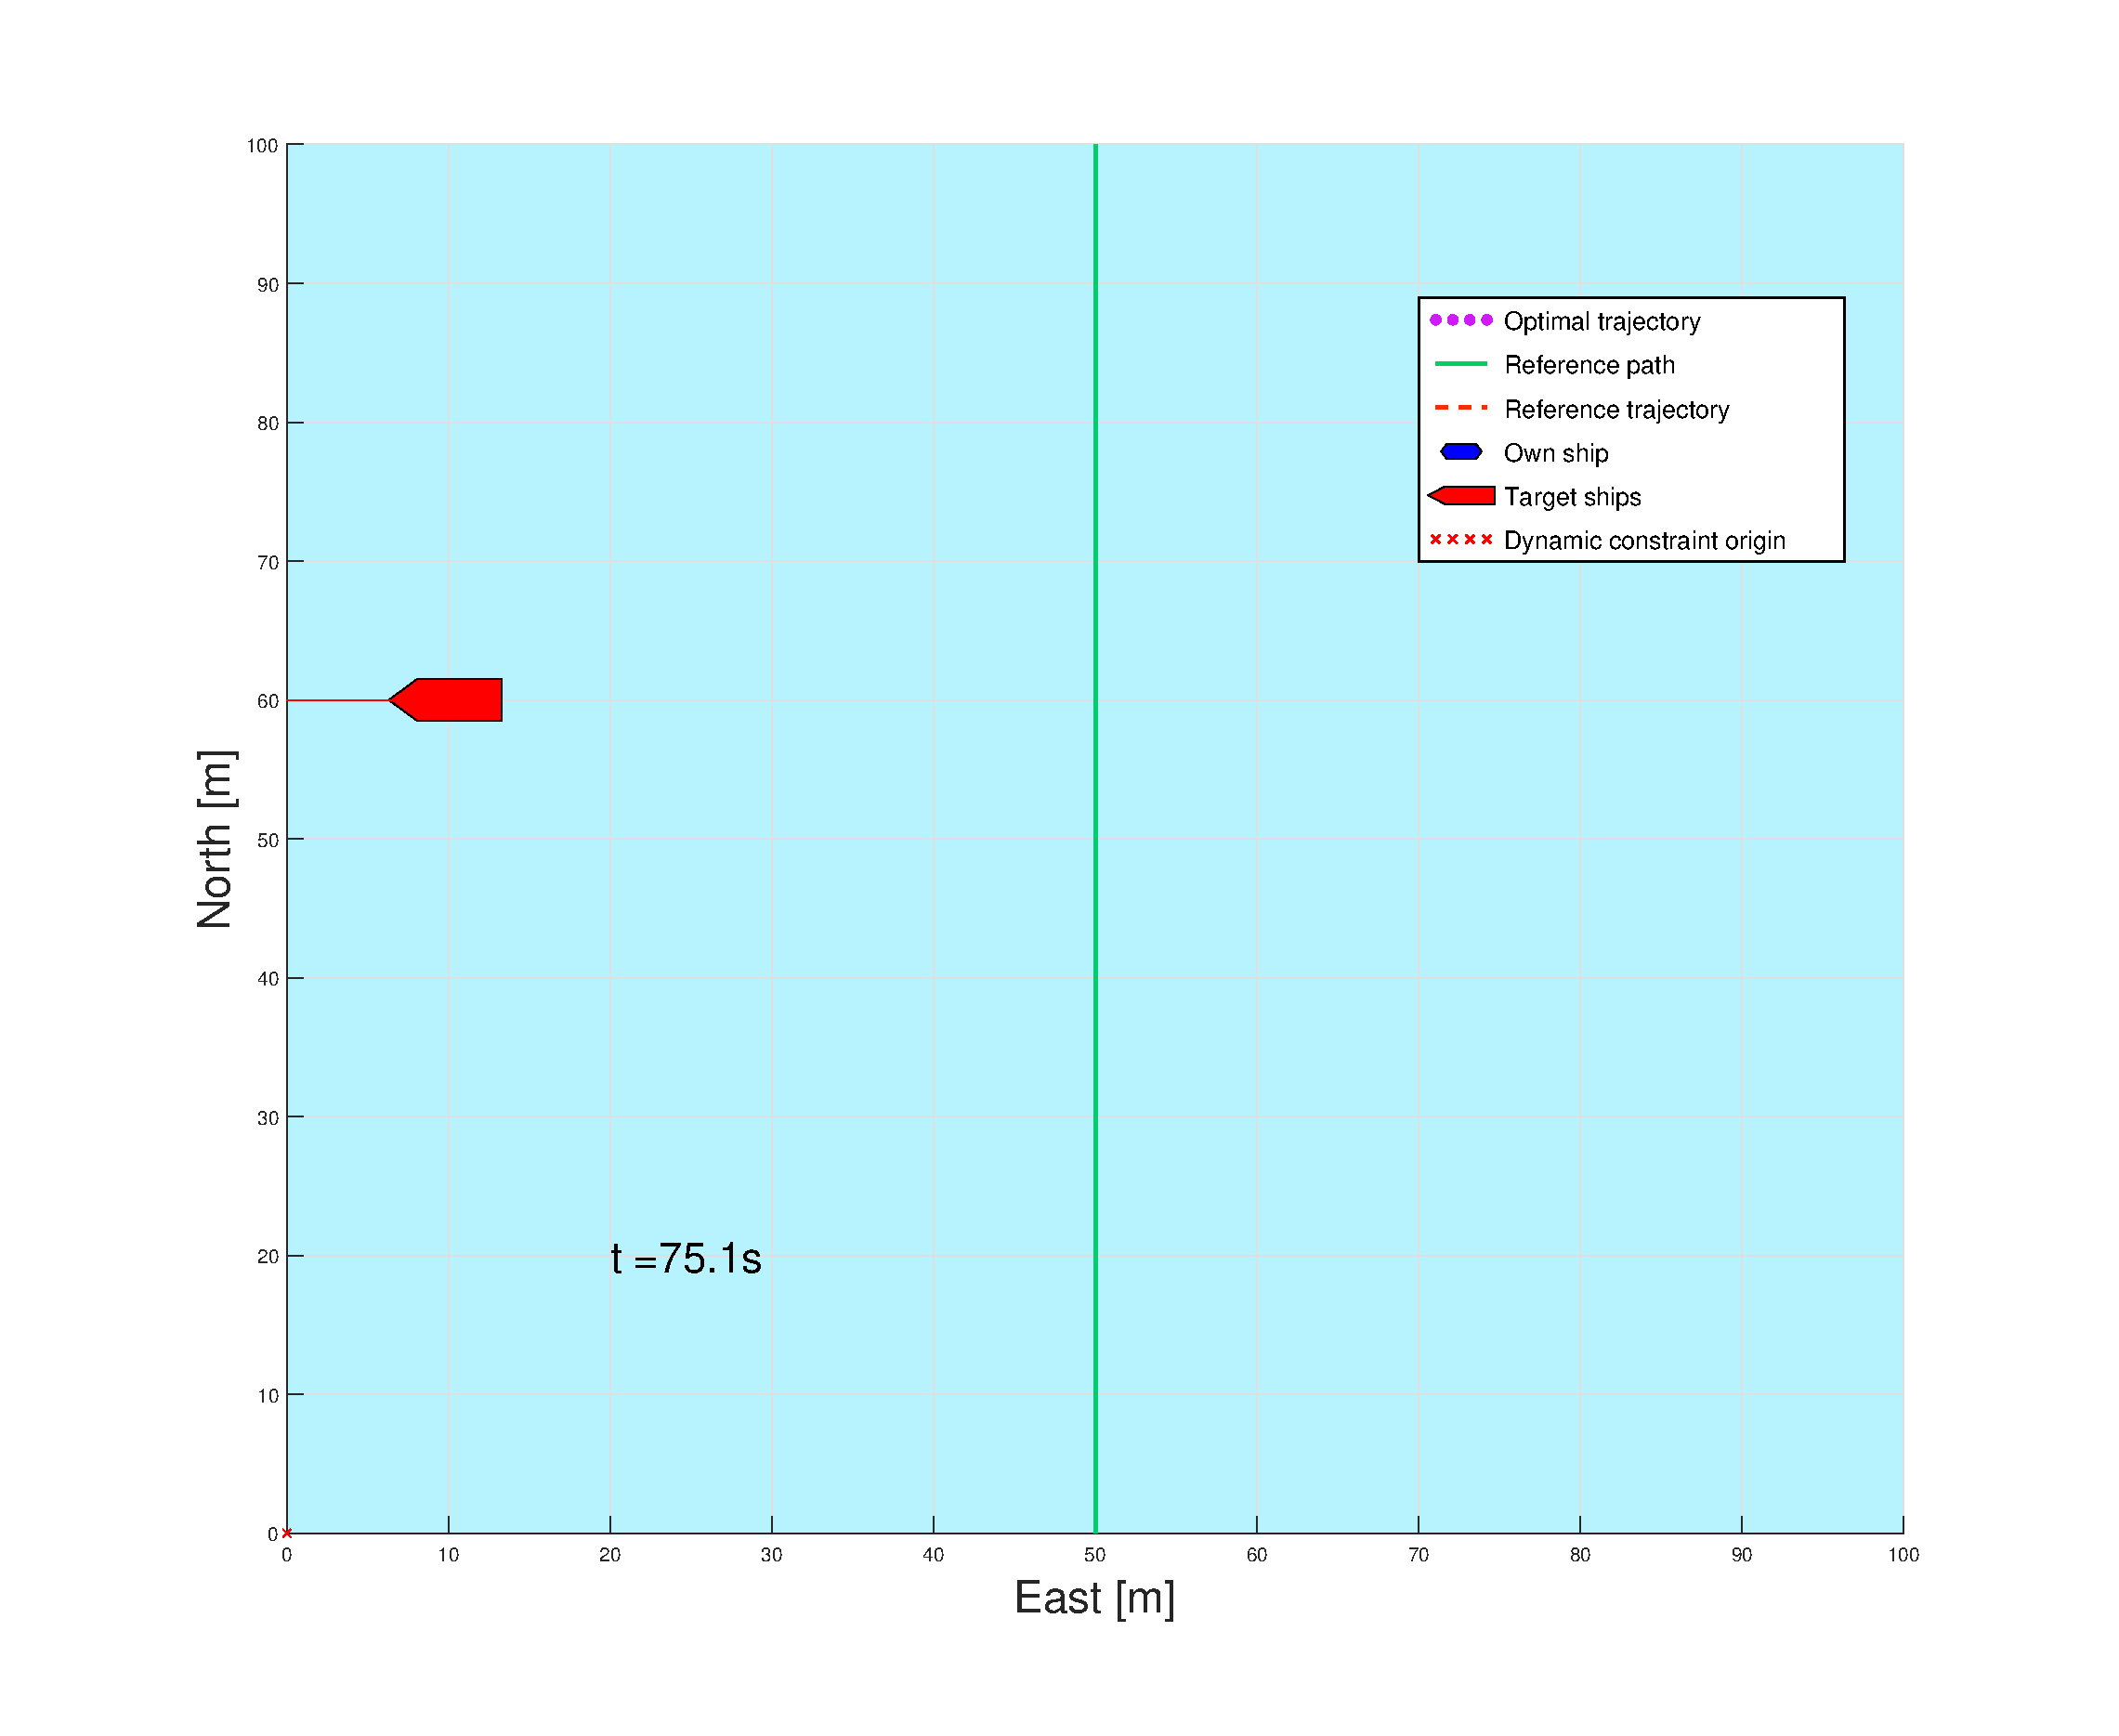
\includegraphics[width=\textwidth]{Images/Figures/enkel_GW/_Simple_1fig999_time=75}
        \subcaption{mhm}
    \end{subfigure}
    \hfill
    \caption{Simple Give Way Without Prediction}
\end{figure}



\subsubsection{Simple Stand On}
\begin{itemize}
    \item This scenario assumes that the \gls{Ts} plays nice and attempts to follow the \gls{COLREGs} rules.
    \item When using simple prediction the optimal path is pushed towads port side behind the \gls{Ts}, and as the \gls{Ts} begins to turn the \gls{OS} is dragged along by the movement of the constraints.
    \item This is actually quite unrealistic, there is no reason to assume the \gls{Ts} would continue to yield after observing the \gls{OS} change course like this. It's also a bad result for simple prediction because the behaviour can cause confusion\\
    for other navigator.
    \item The author realized late that the way prediction is done of the \gls{Ts} is not entirely consistent with the way prediction is handled internally in the algorithm. In the algorithm waypoints are used to predict \gls{Ts}s trajectories, which is not neccessary\\
    the exact same trajectory as the \gls{Ts} ends up following. 
    \item In order to get the \gls{Ts} to comply with expected \gls{COLREGs} behaviour a waypoint was placed some meters south of the \gls{OS} position at the would be \gls{tCPA}. This waypoint would obviously not exist in a normal transit situation and so\\
    this scenario is actually a bit of a cheat in regards to how prediction is argued for in prior chapters.
    \item The result is still interesting, for this scenario only we can exchange the advanced prediction result with a fully accurate prediction, and the result for simple prediction would hold for the current algorithm in all cases.
\end{itemize}

\clearpage
\begin{figure}[!b]
    \begin{subfigure}[b]{0.49\textwidth}
        \centering
        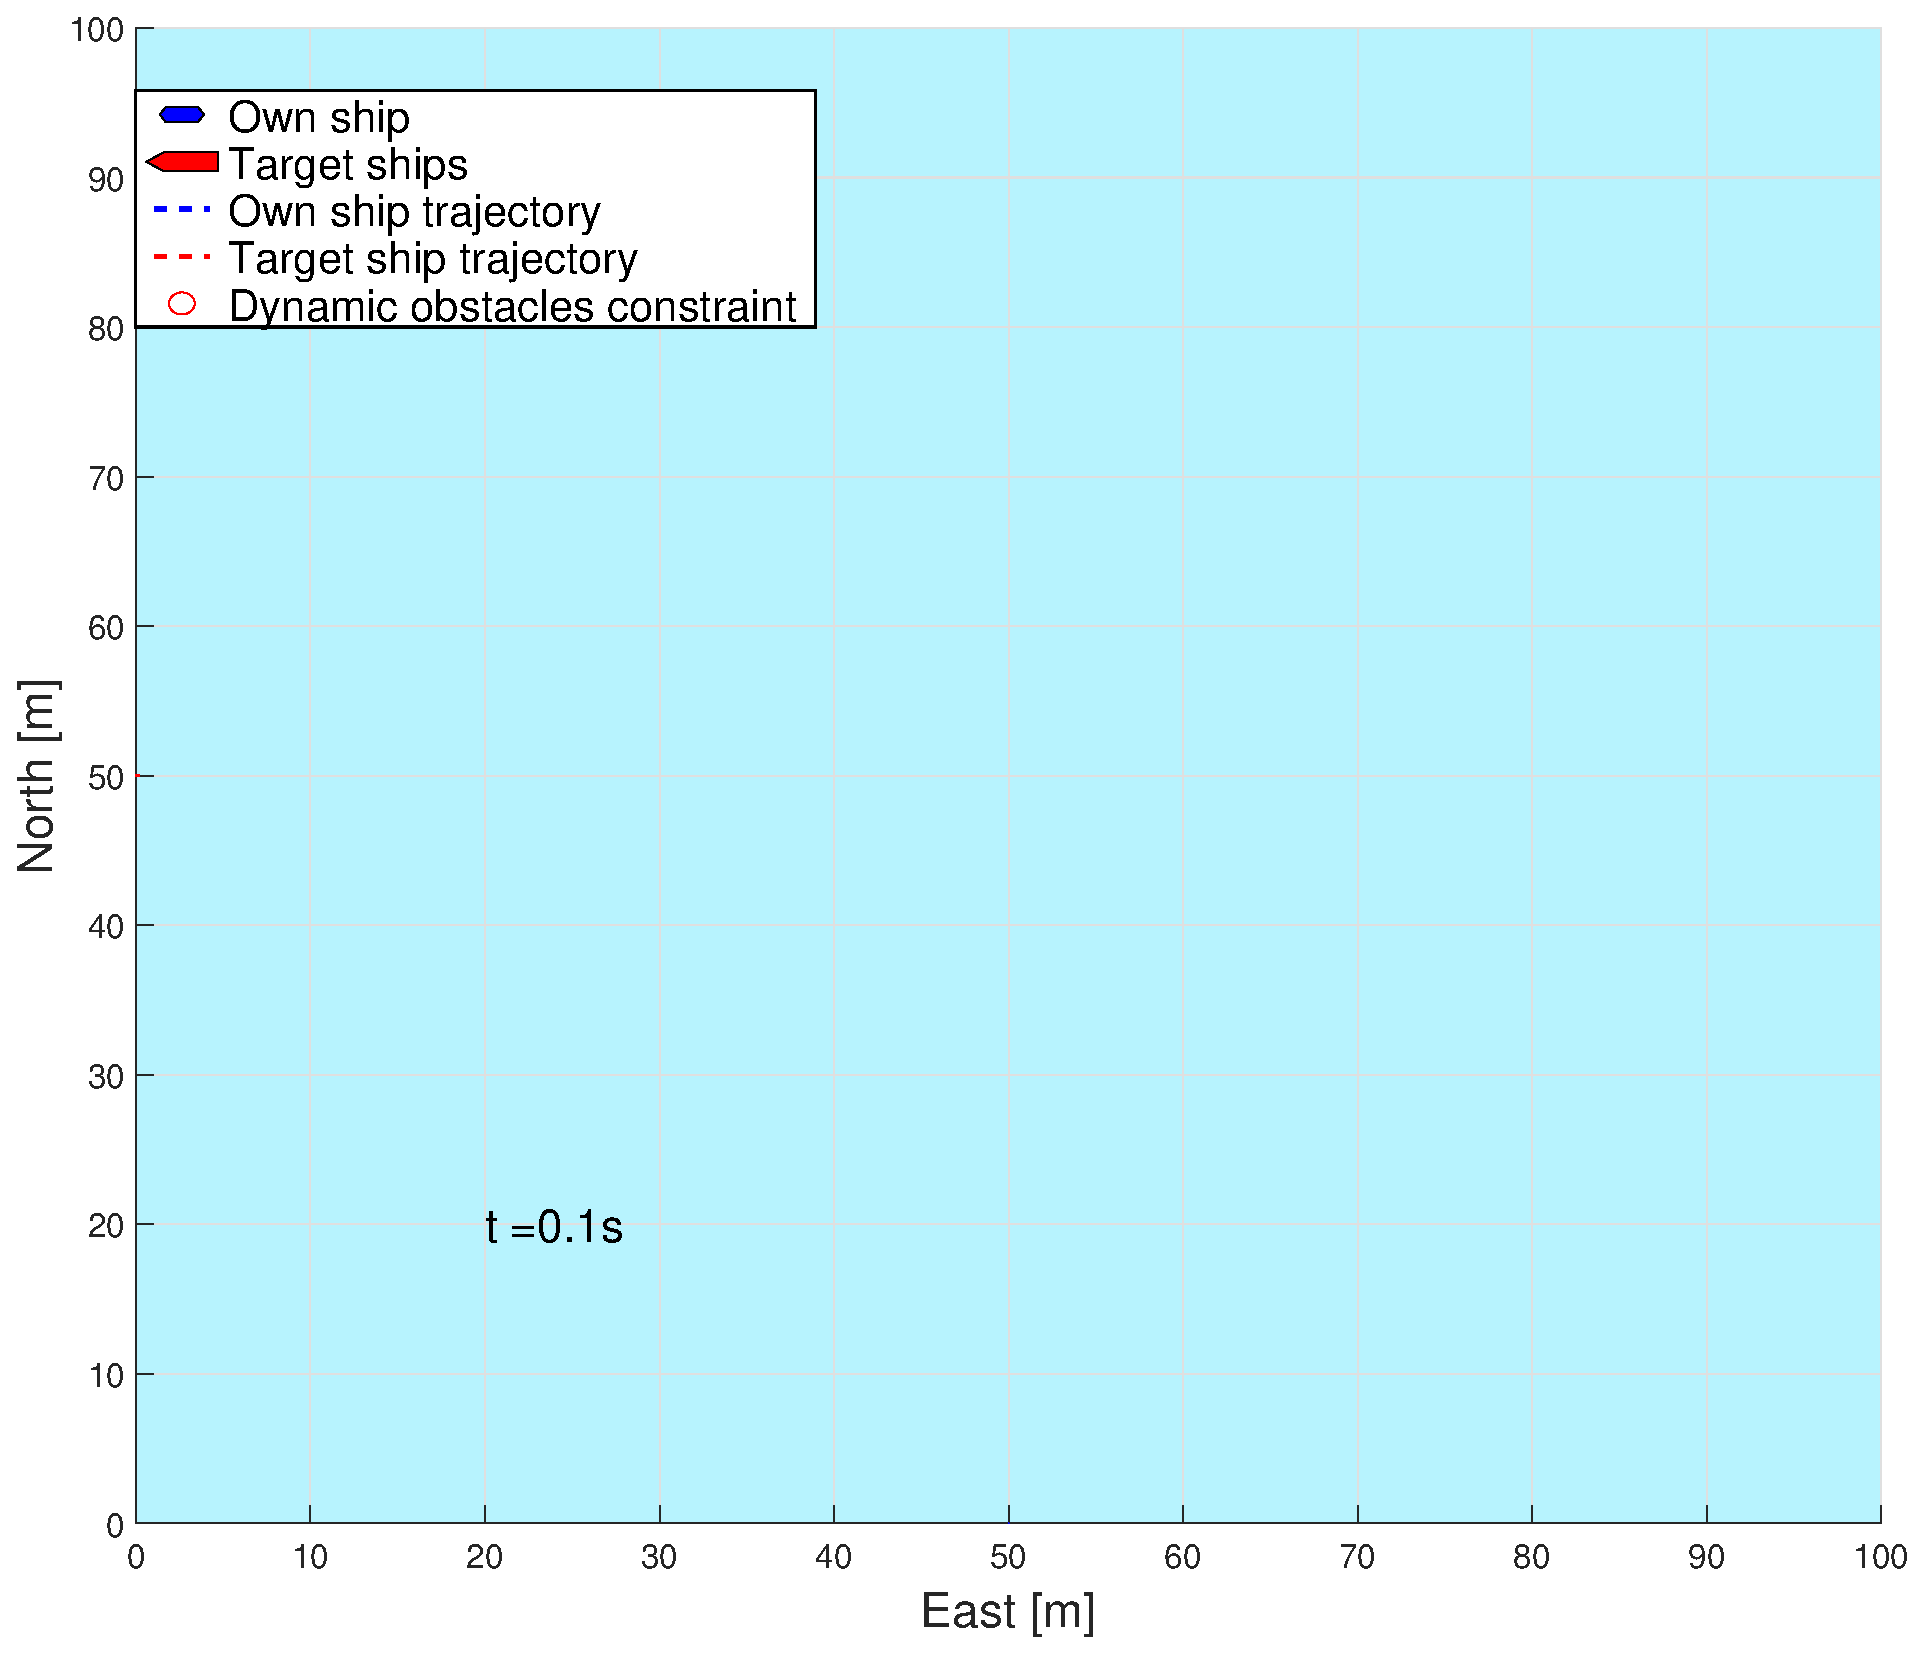
\includegraphics[width=\textwidth]{Images/Figures/enkel_SO/_Simple_0fig1_time=0}
        \subcaption{caption}
    \end{subfigure}
    \hfill
    \begin{subfigure}[b]{0.499\textwidth}
        \centering
        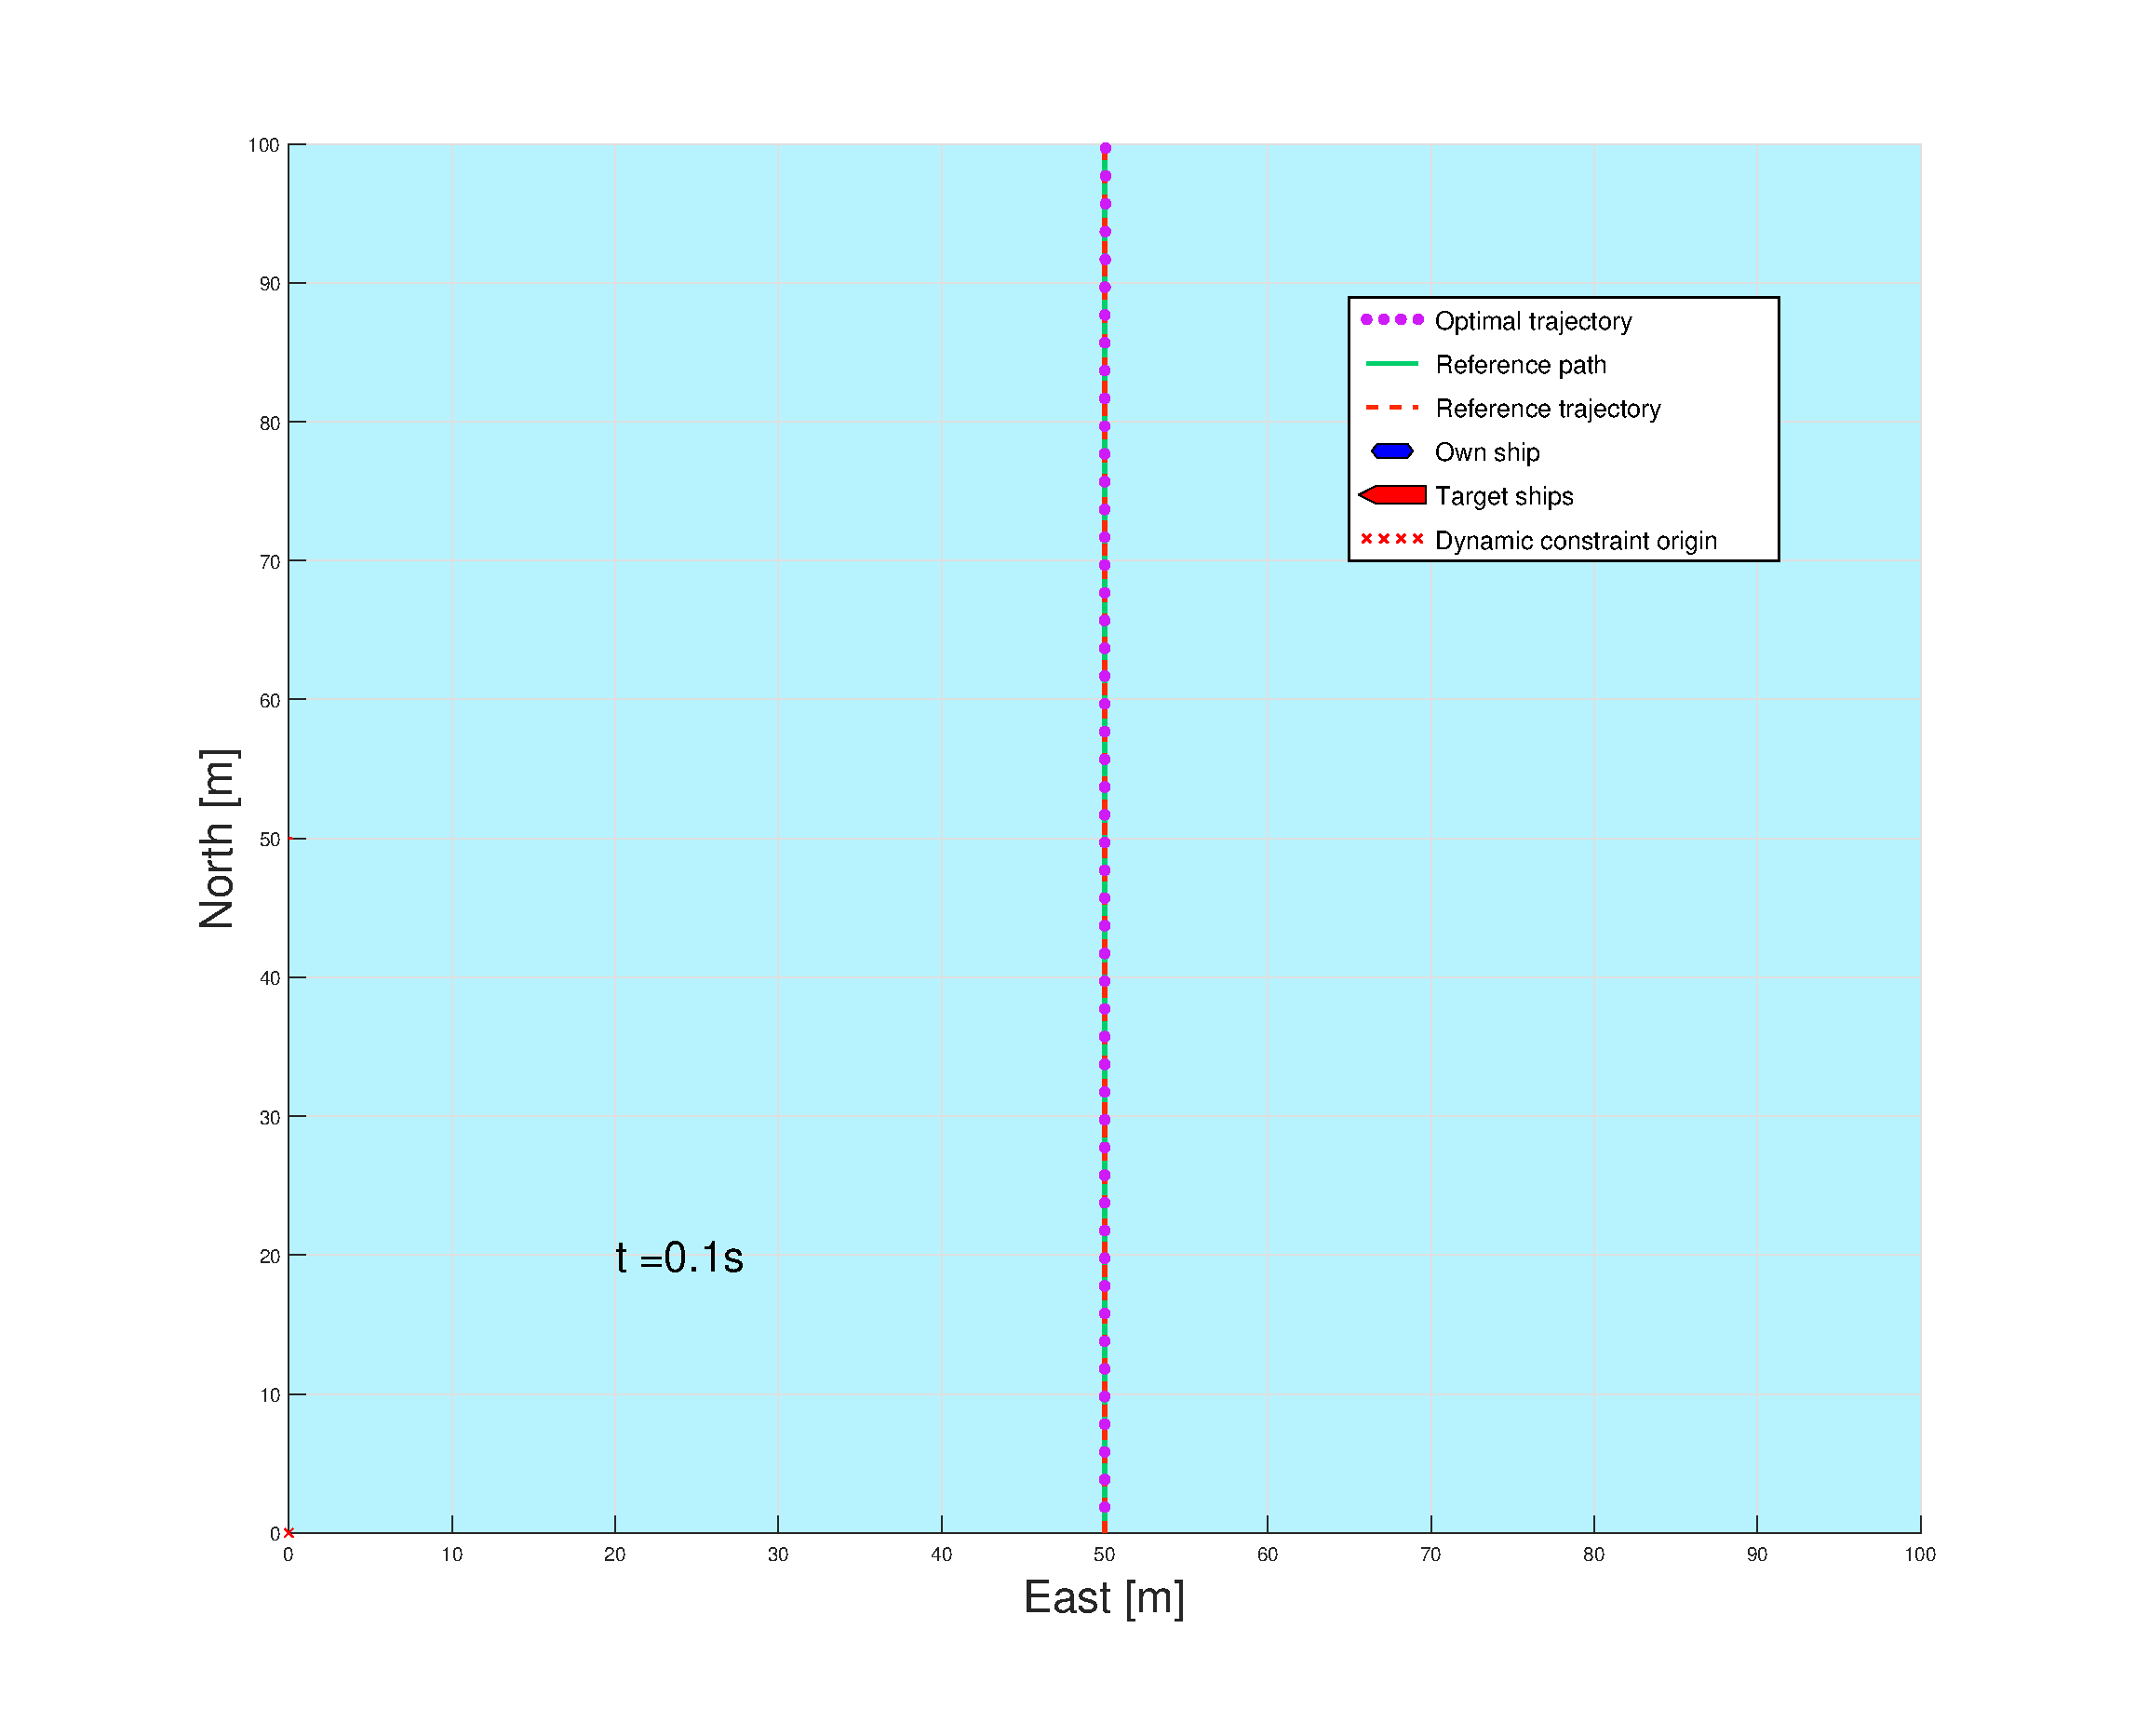
\includegraphics[width=\textwidth]{Images/Figures/enkel_SO/_Simple_0fig999_time=0}
        \subcaption{mhm}
    \end{subfigure}
    \hfill
    \\
    \begin{subfigure}[b]{0.49\textwidth}
        \centering
        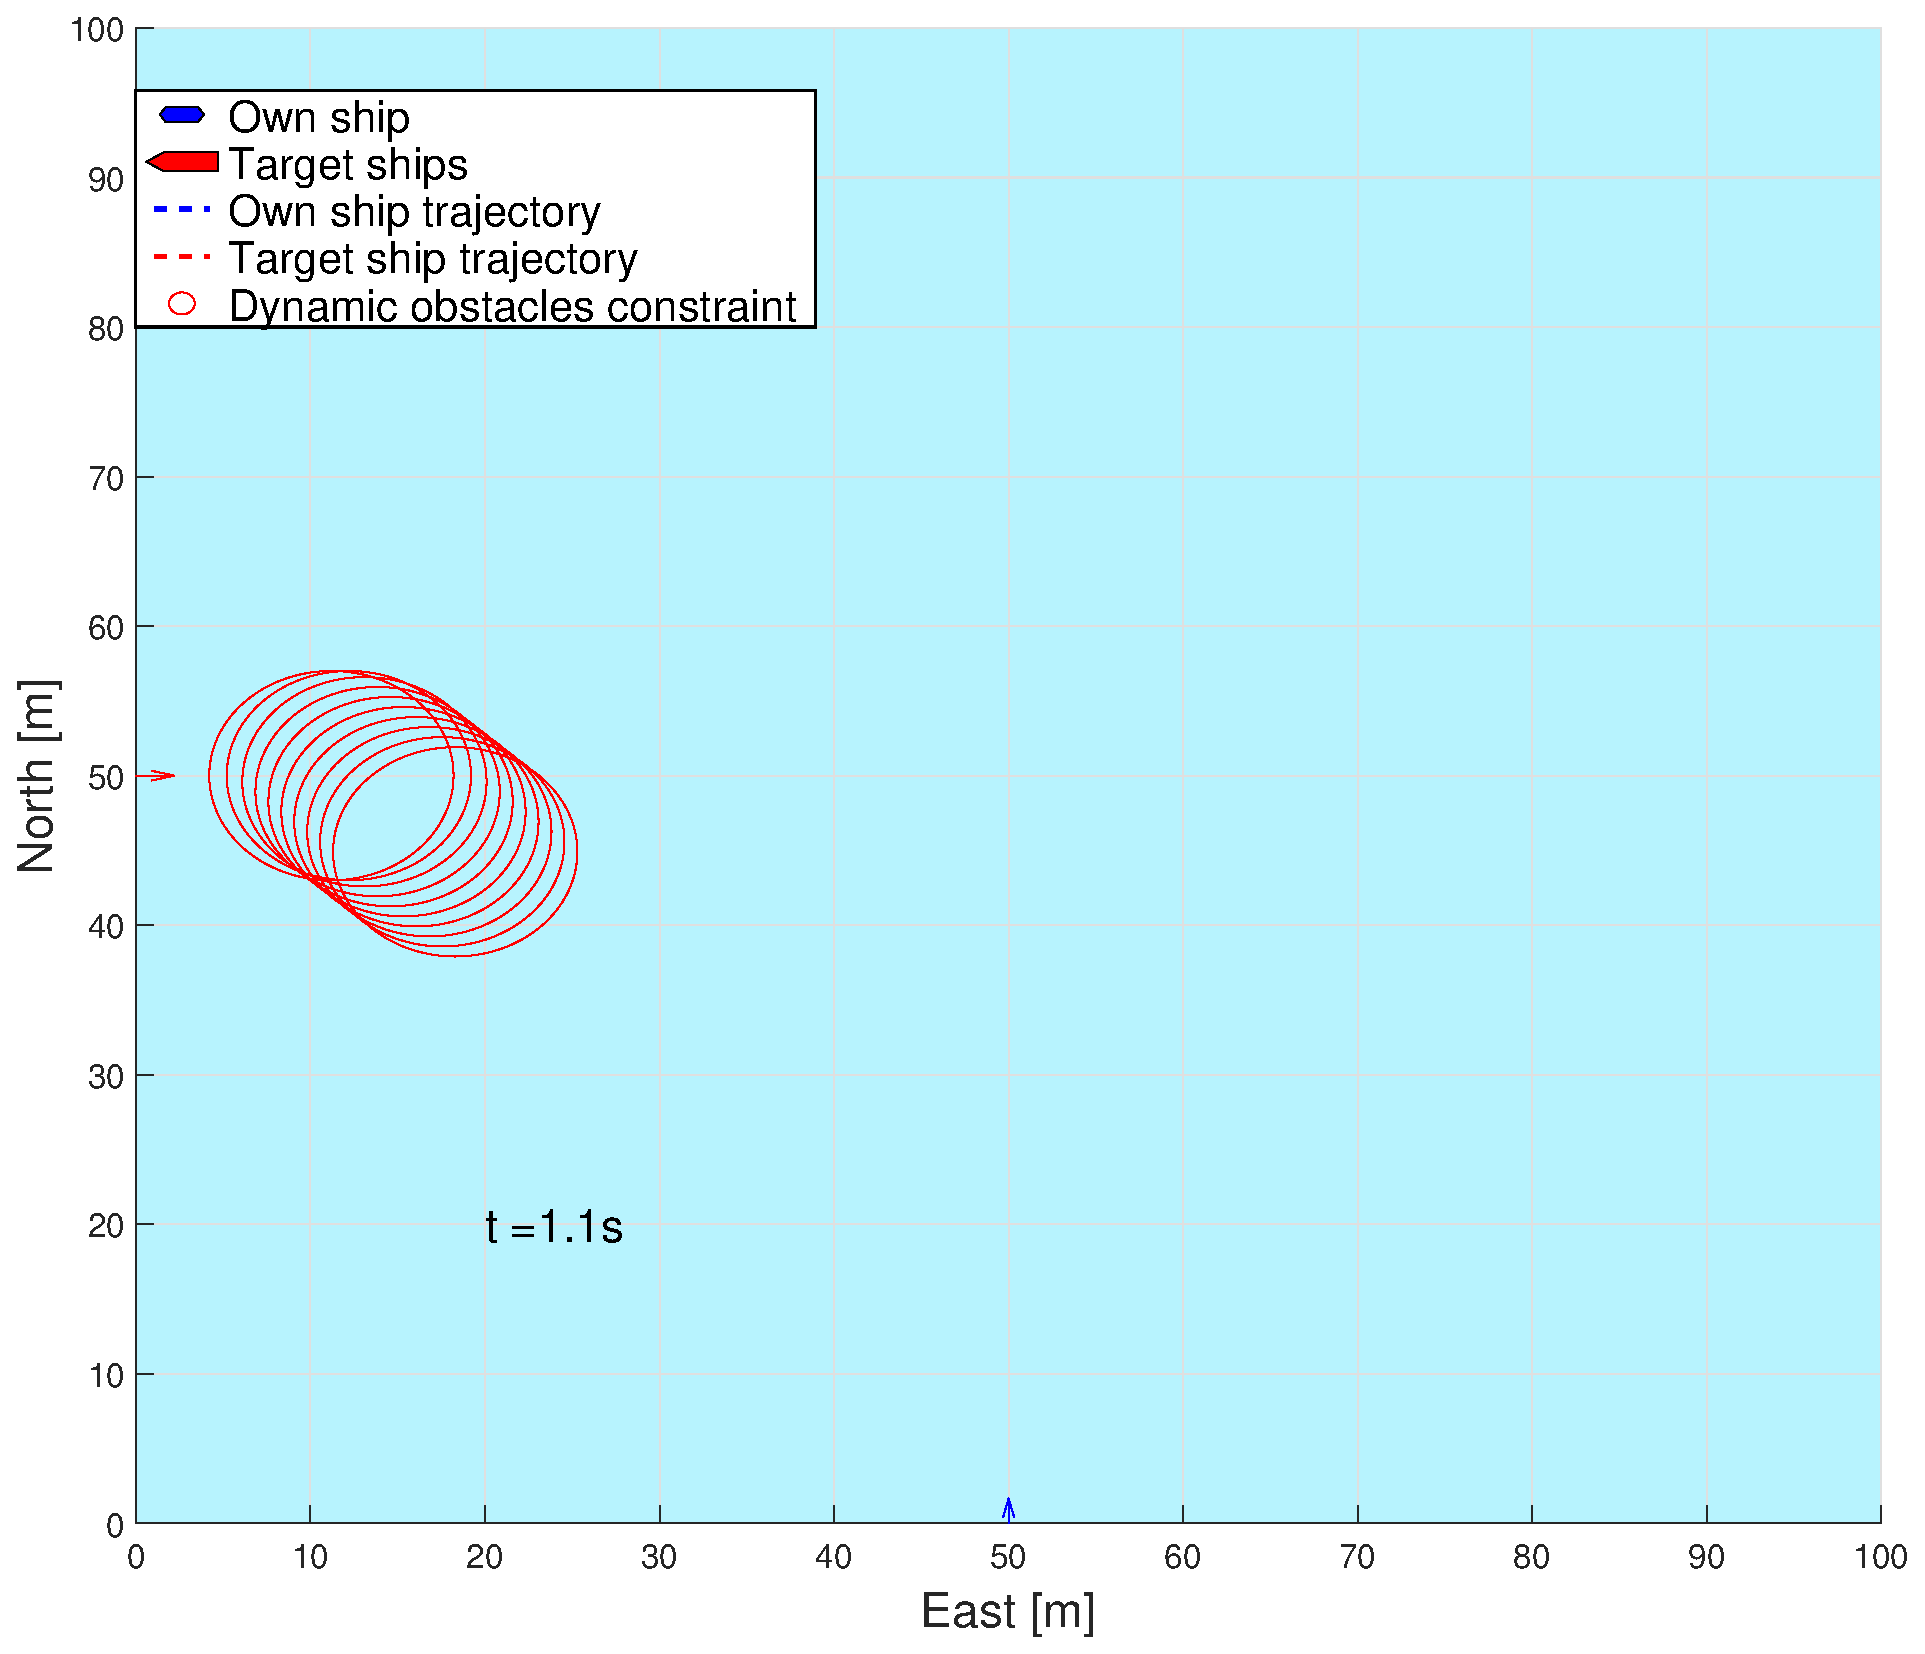
\includegraphics[width=\textwidth]{Images/Figures/enkel_SO/_Simple_0fig1_time=1}
        \subcaption{caption}
    \end{subfigure}
    \hfill
    \begin{subfigure}[b]{0.499\textwidth}
        \centering
        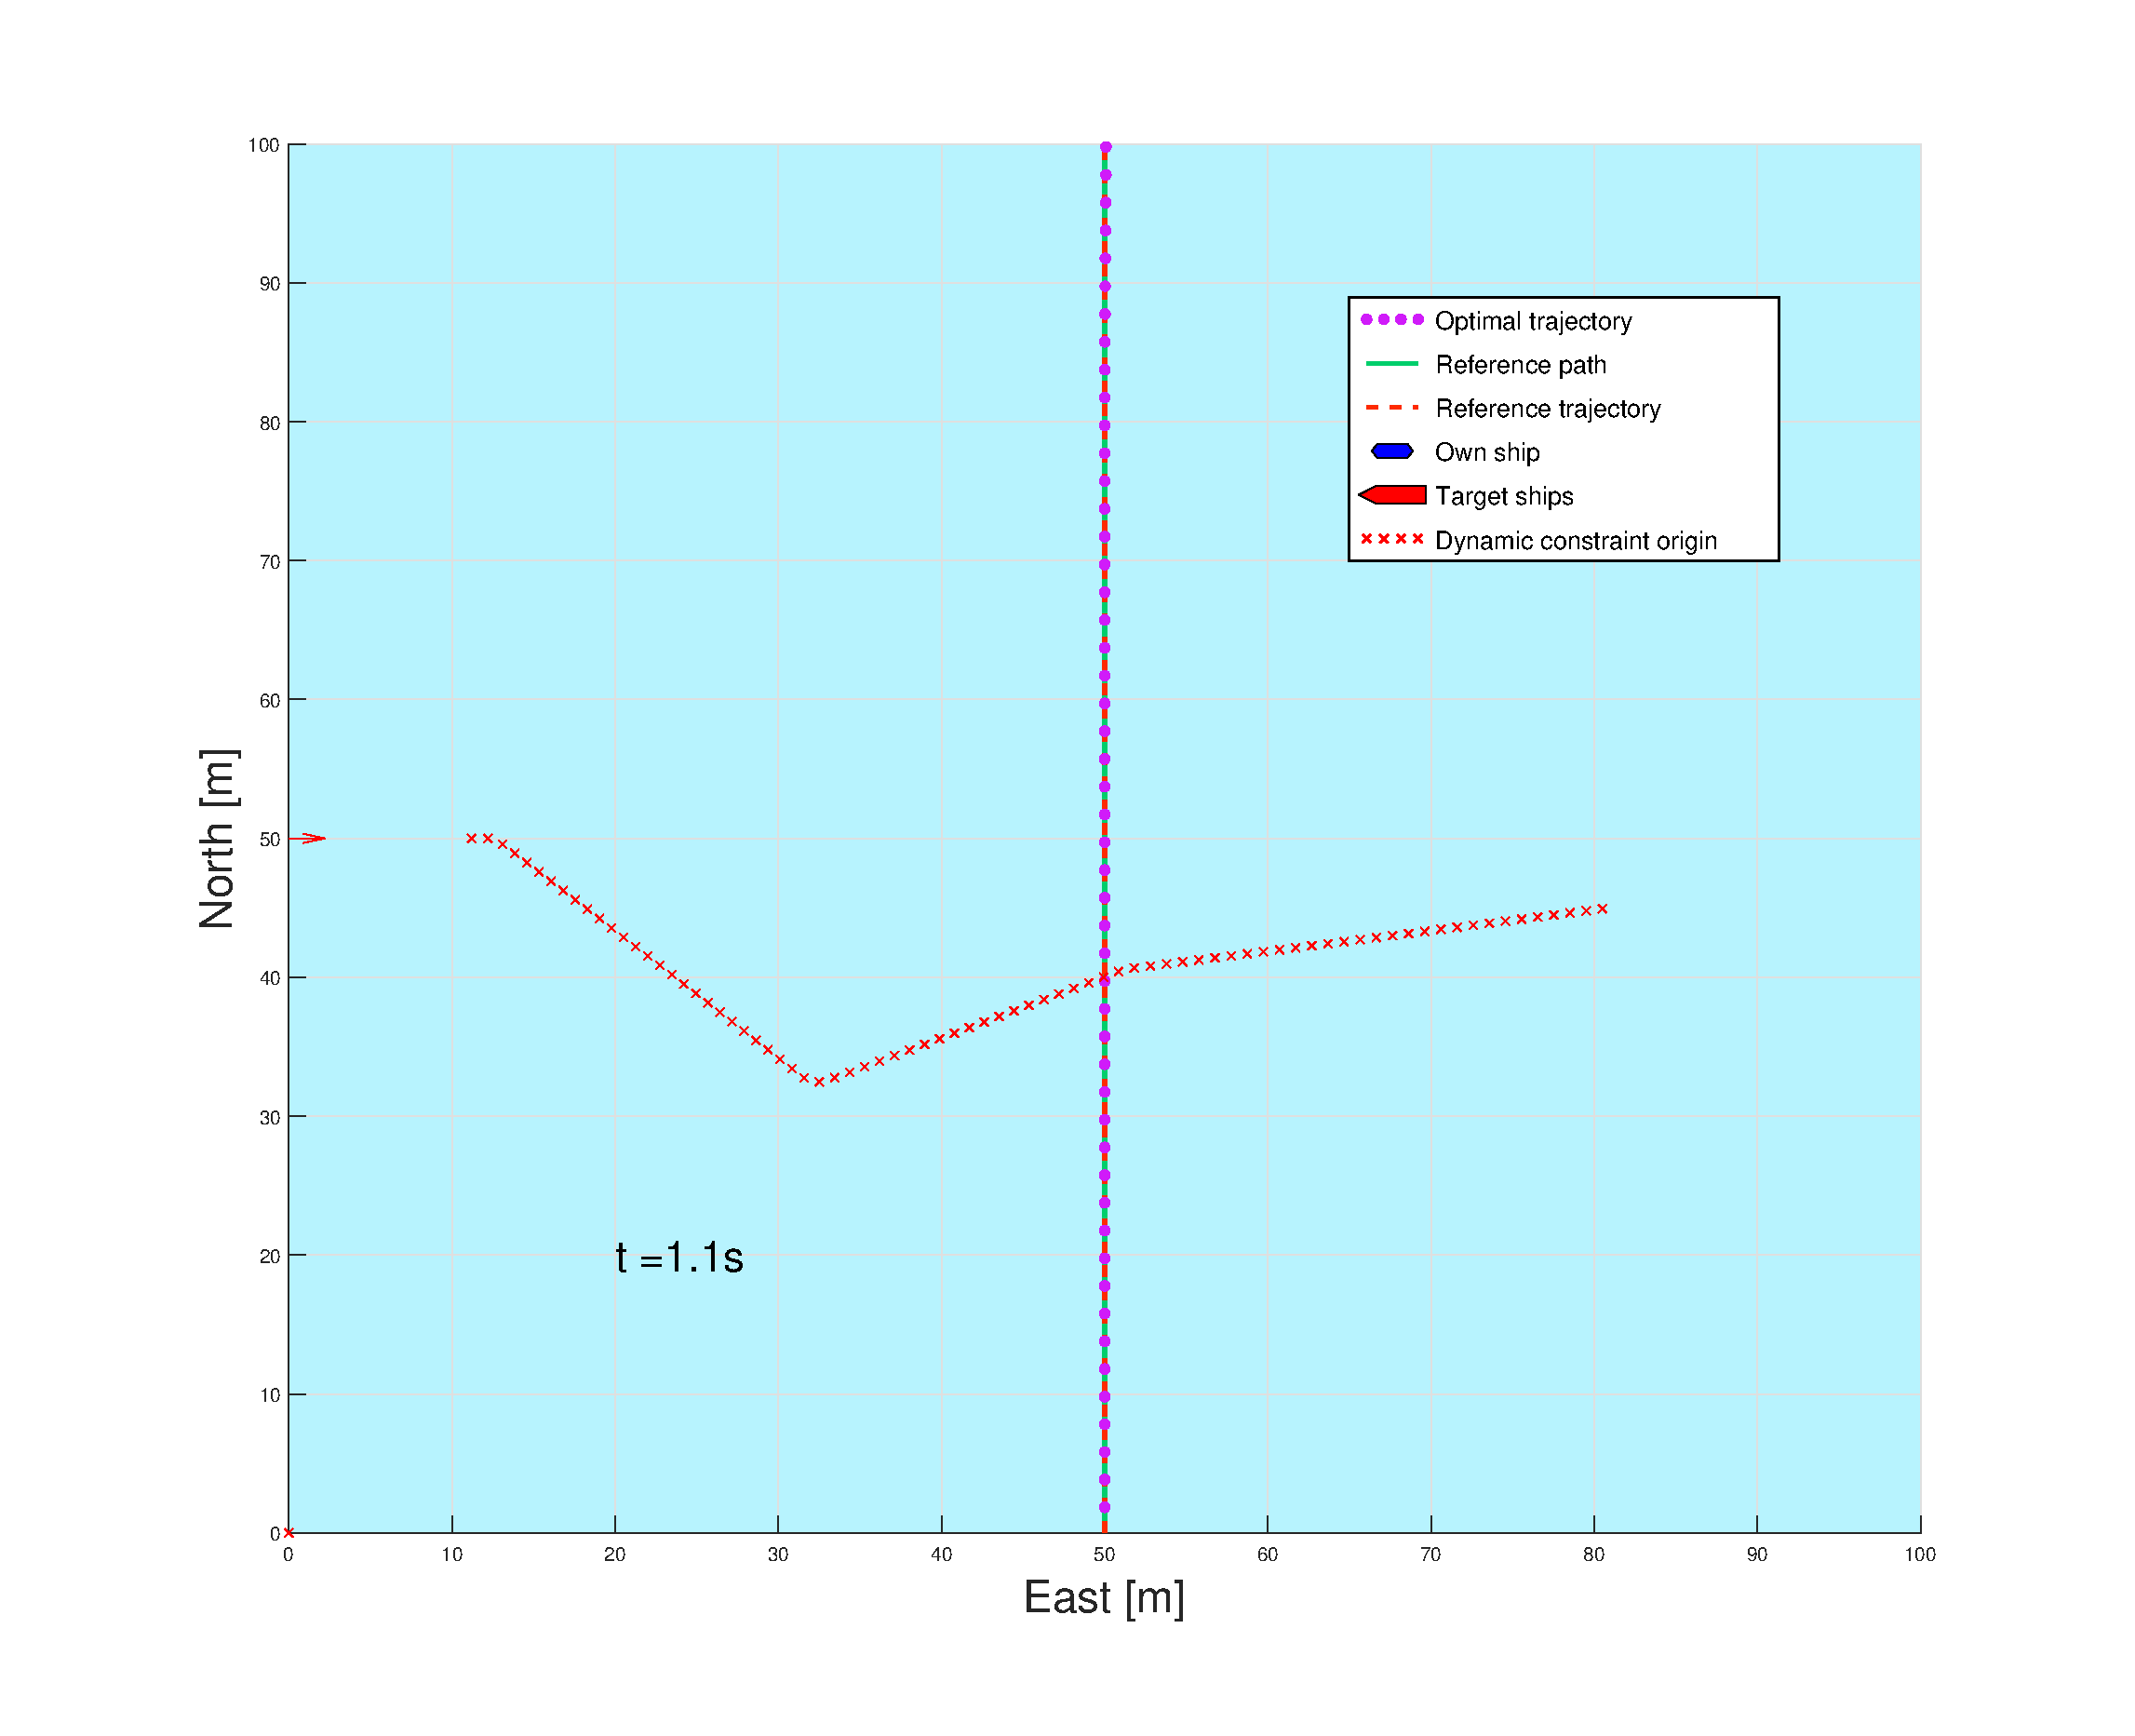
\includegraphics[width=\textwidth]{Images/Figures/enkel_SO/_Simple_0fig999_time=1}
        \subcaption{mhm}
    \end{subfigure}
    \hfill
    \\
    \begin{subfigure}[b]{0.49\textwidth}
        \centering
        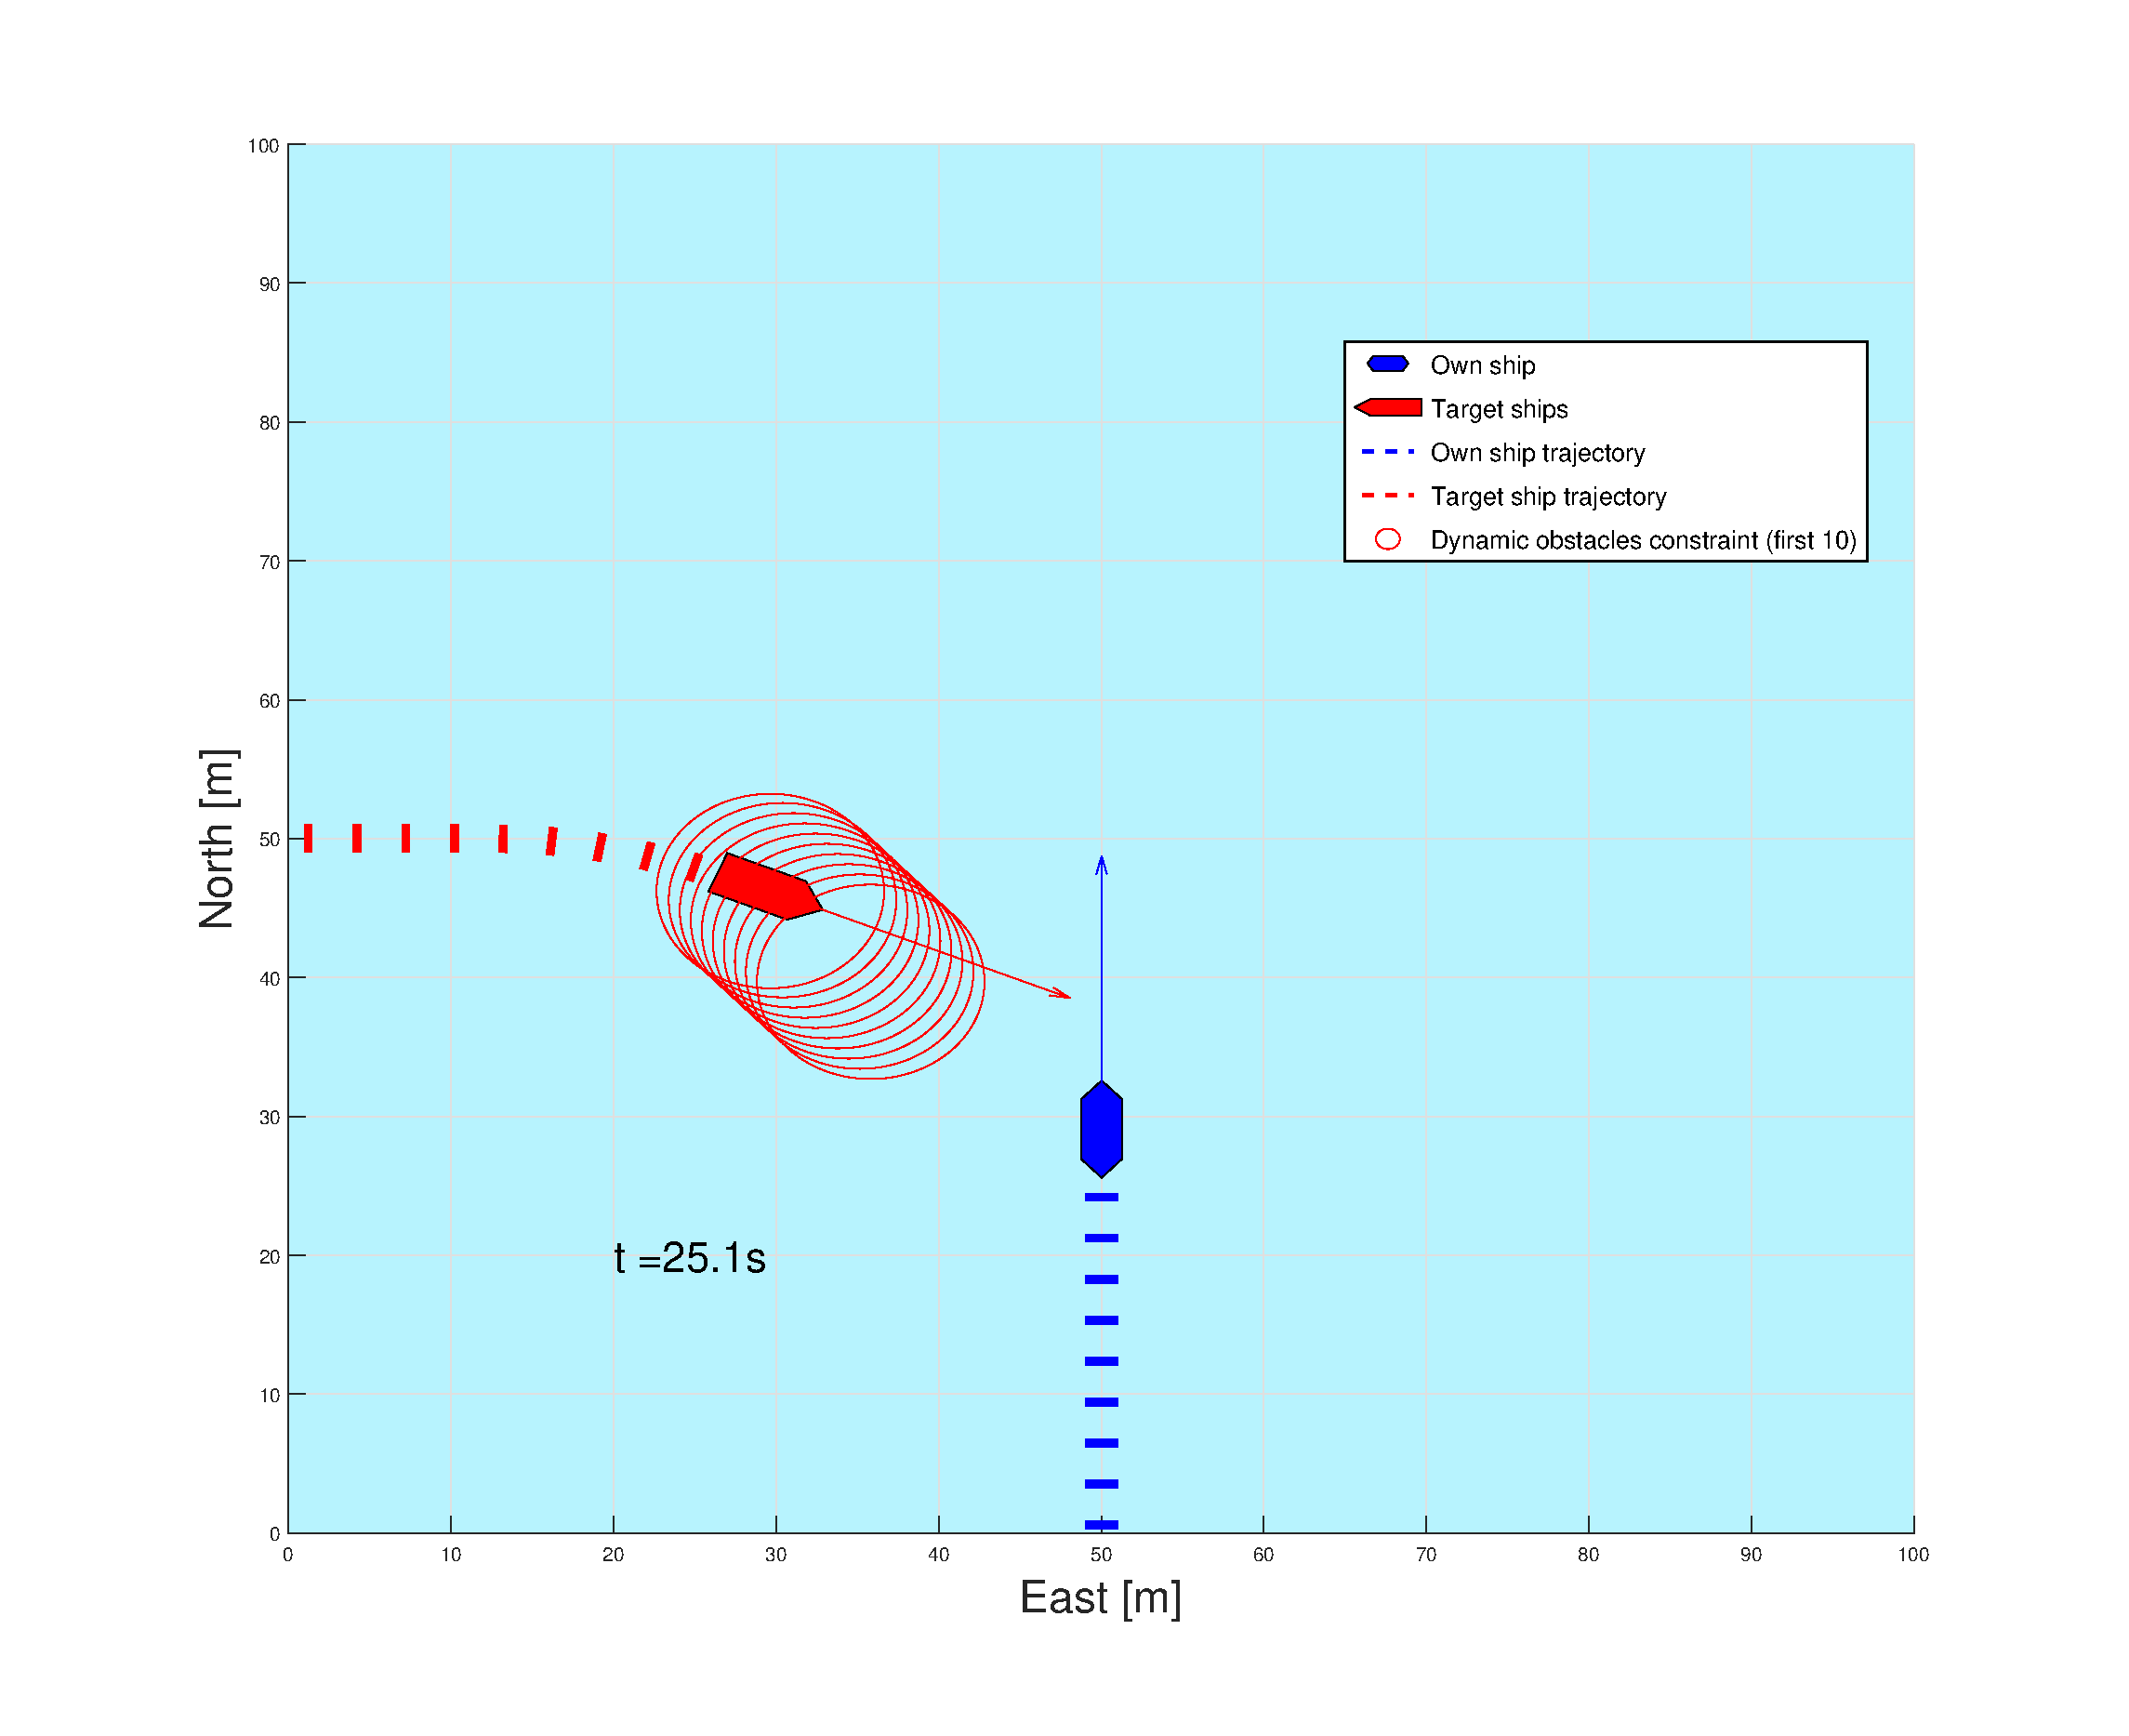
\includegraphics[width=\textwidth]{Images/Figures/enkel_SO/_Simple_0fig1_time=25}
        \subcaption{caption}
    \end{subfigure}
    \hfill
    \begin{subfigure}[b]{0.499\textwidth}
        \centering
        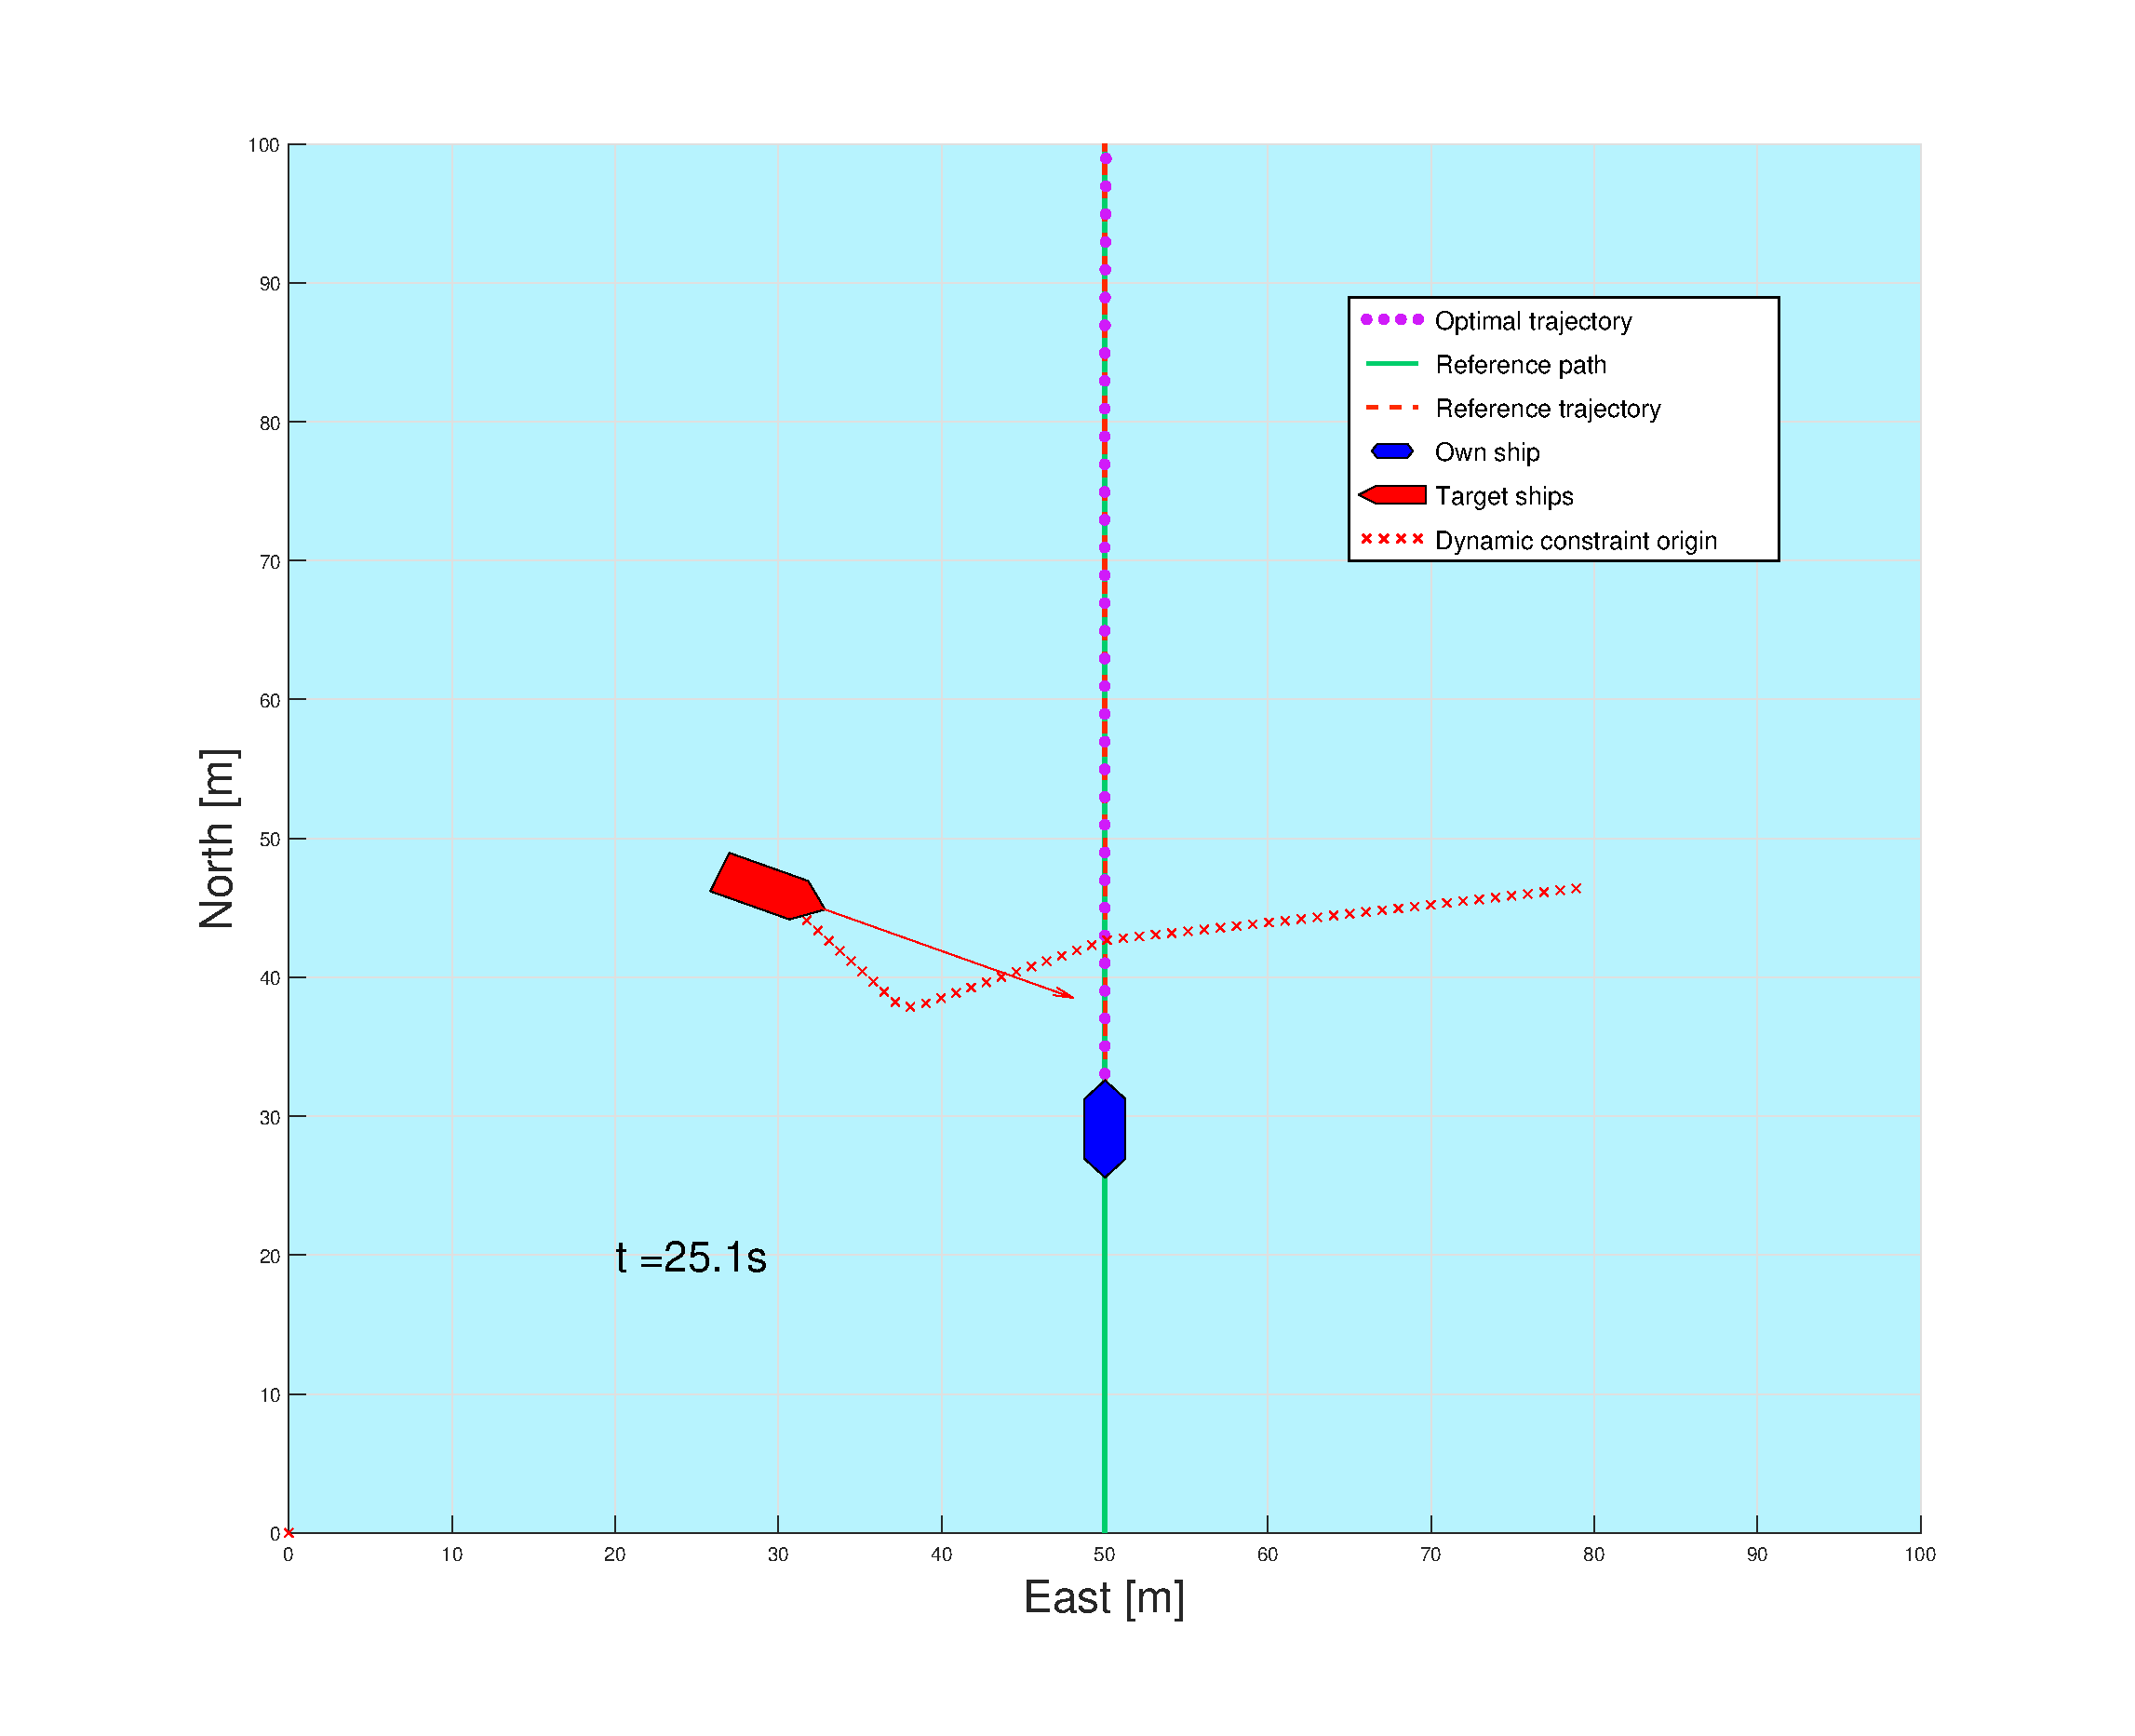
\includegraphics[width=\textwidth]{Images/Figures/enkel_SO/_Simple_0fig999_time=25}
        \subcaption{mhm}
    \end{subfigure}
    \hfill
\end{figure}%
\begin{figure}[ht]\ContinuedFloat
    \begin{subfigure}[b]{0.49\textwidth}
        \centering
        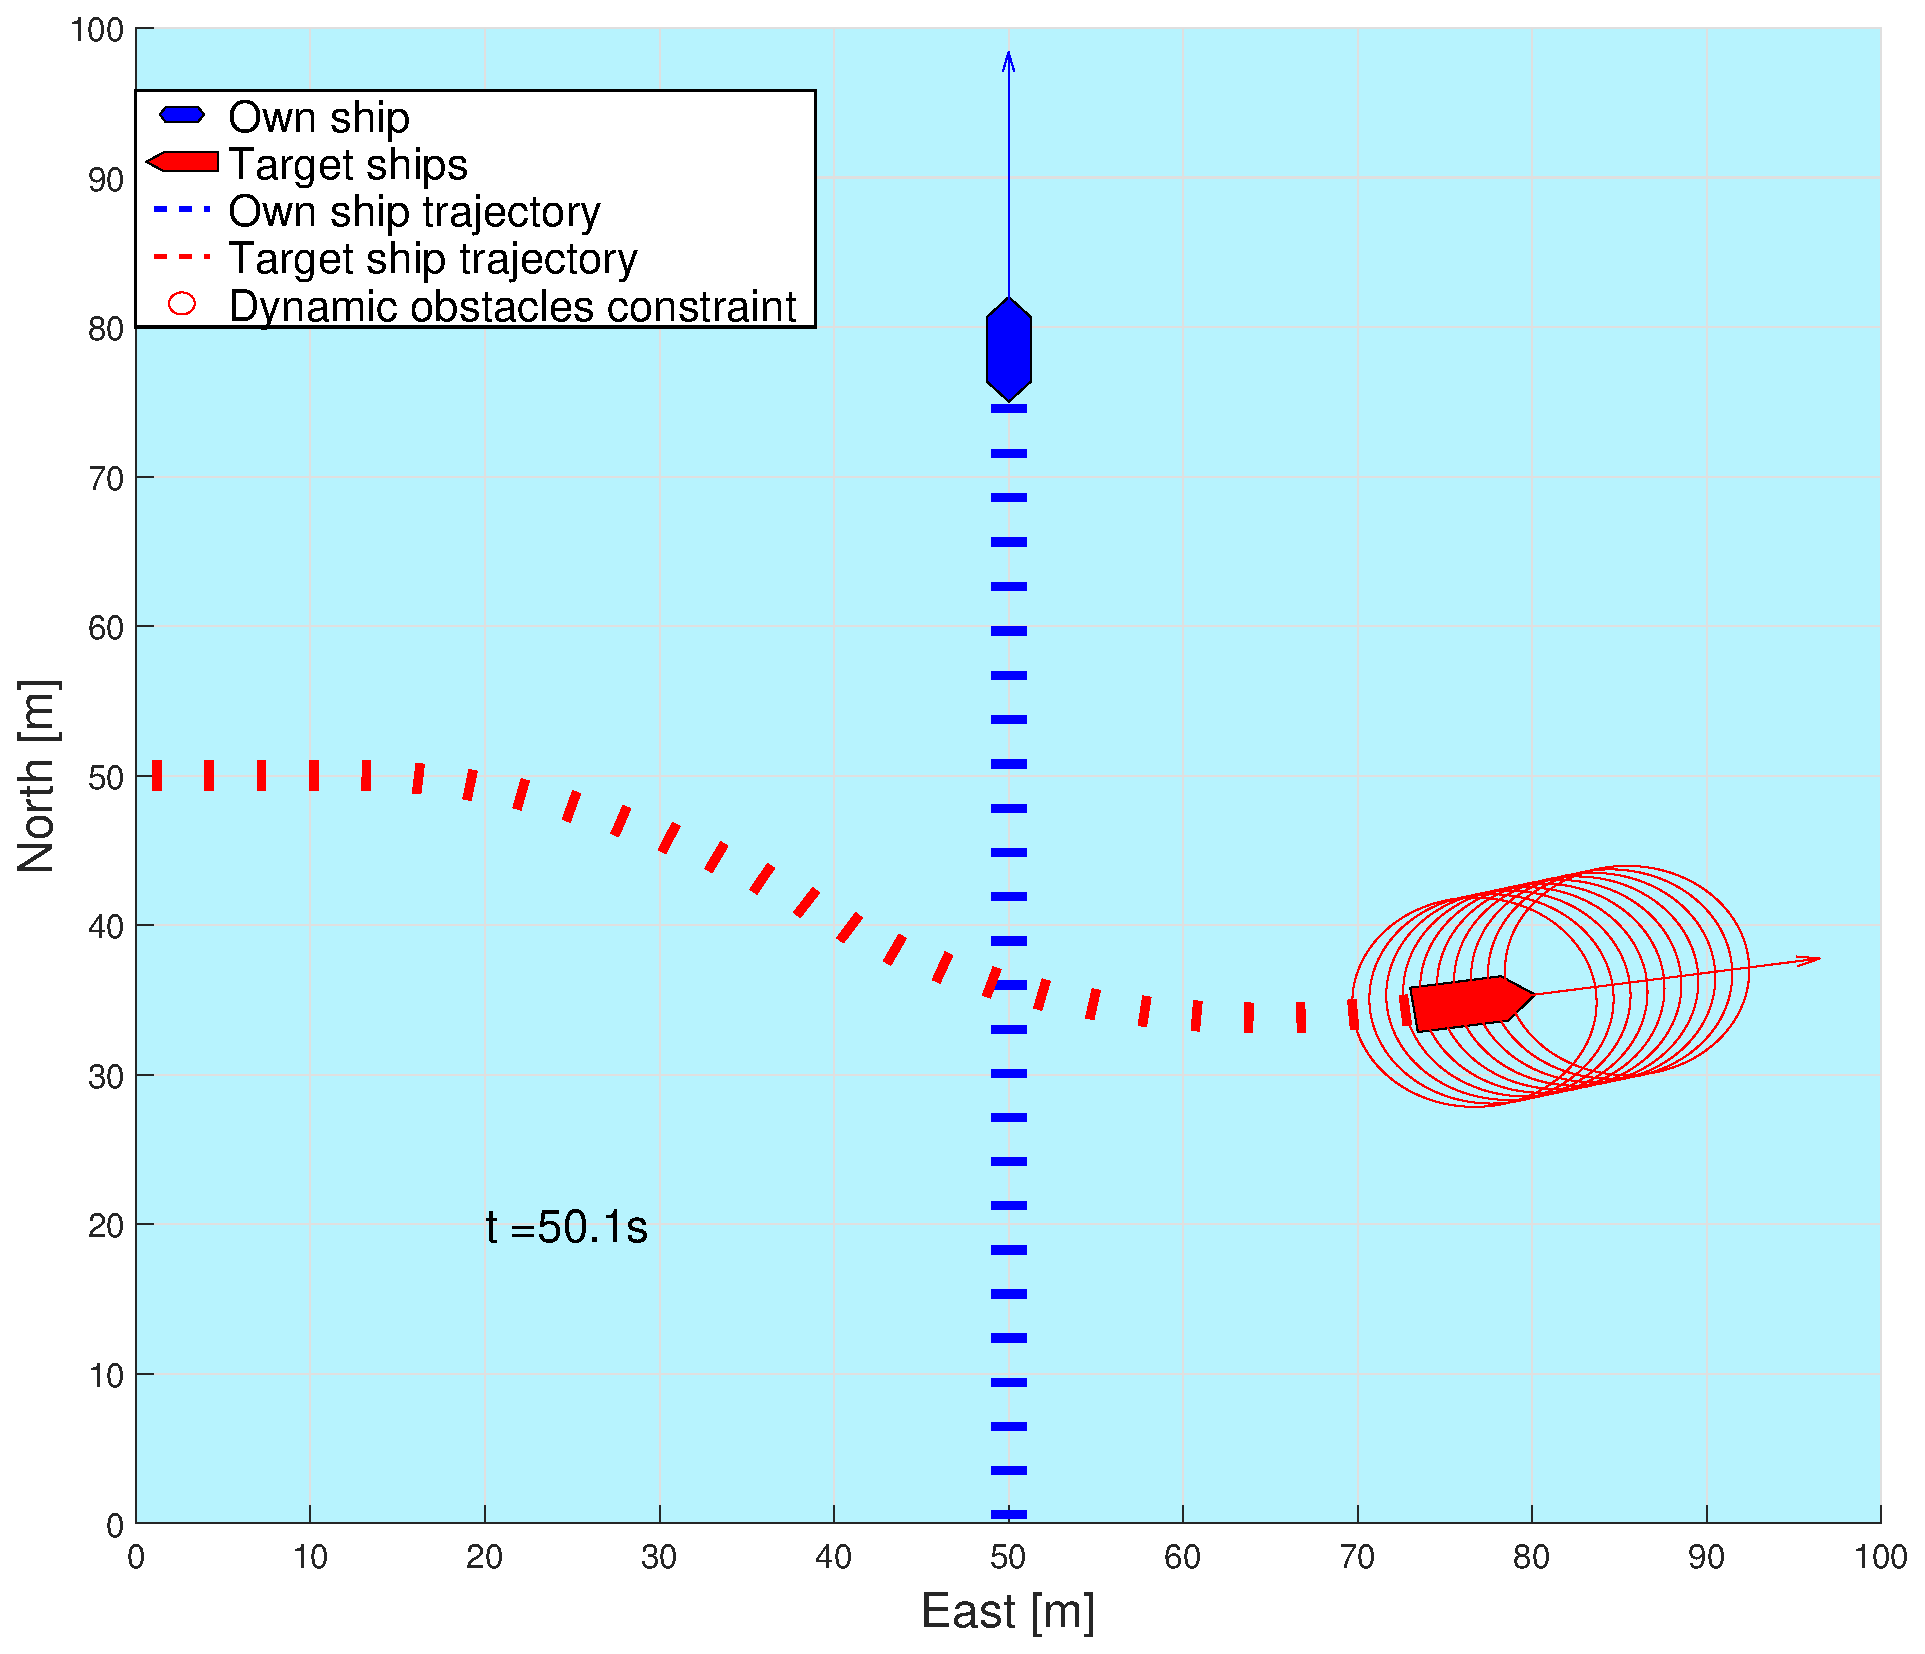
\includegraphics[width=\textwidth]{Images/Figures/enkel_SO/_Simple_0fig1_time=50}
        \subcaption{caption}
    \end{subfigure}
    \hfill
    \begin{subfigure}[b]{0.499\textwidth}
        \centering
        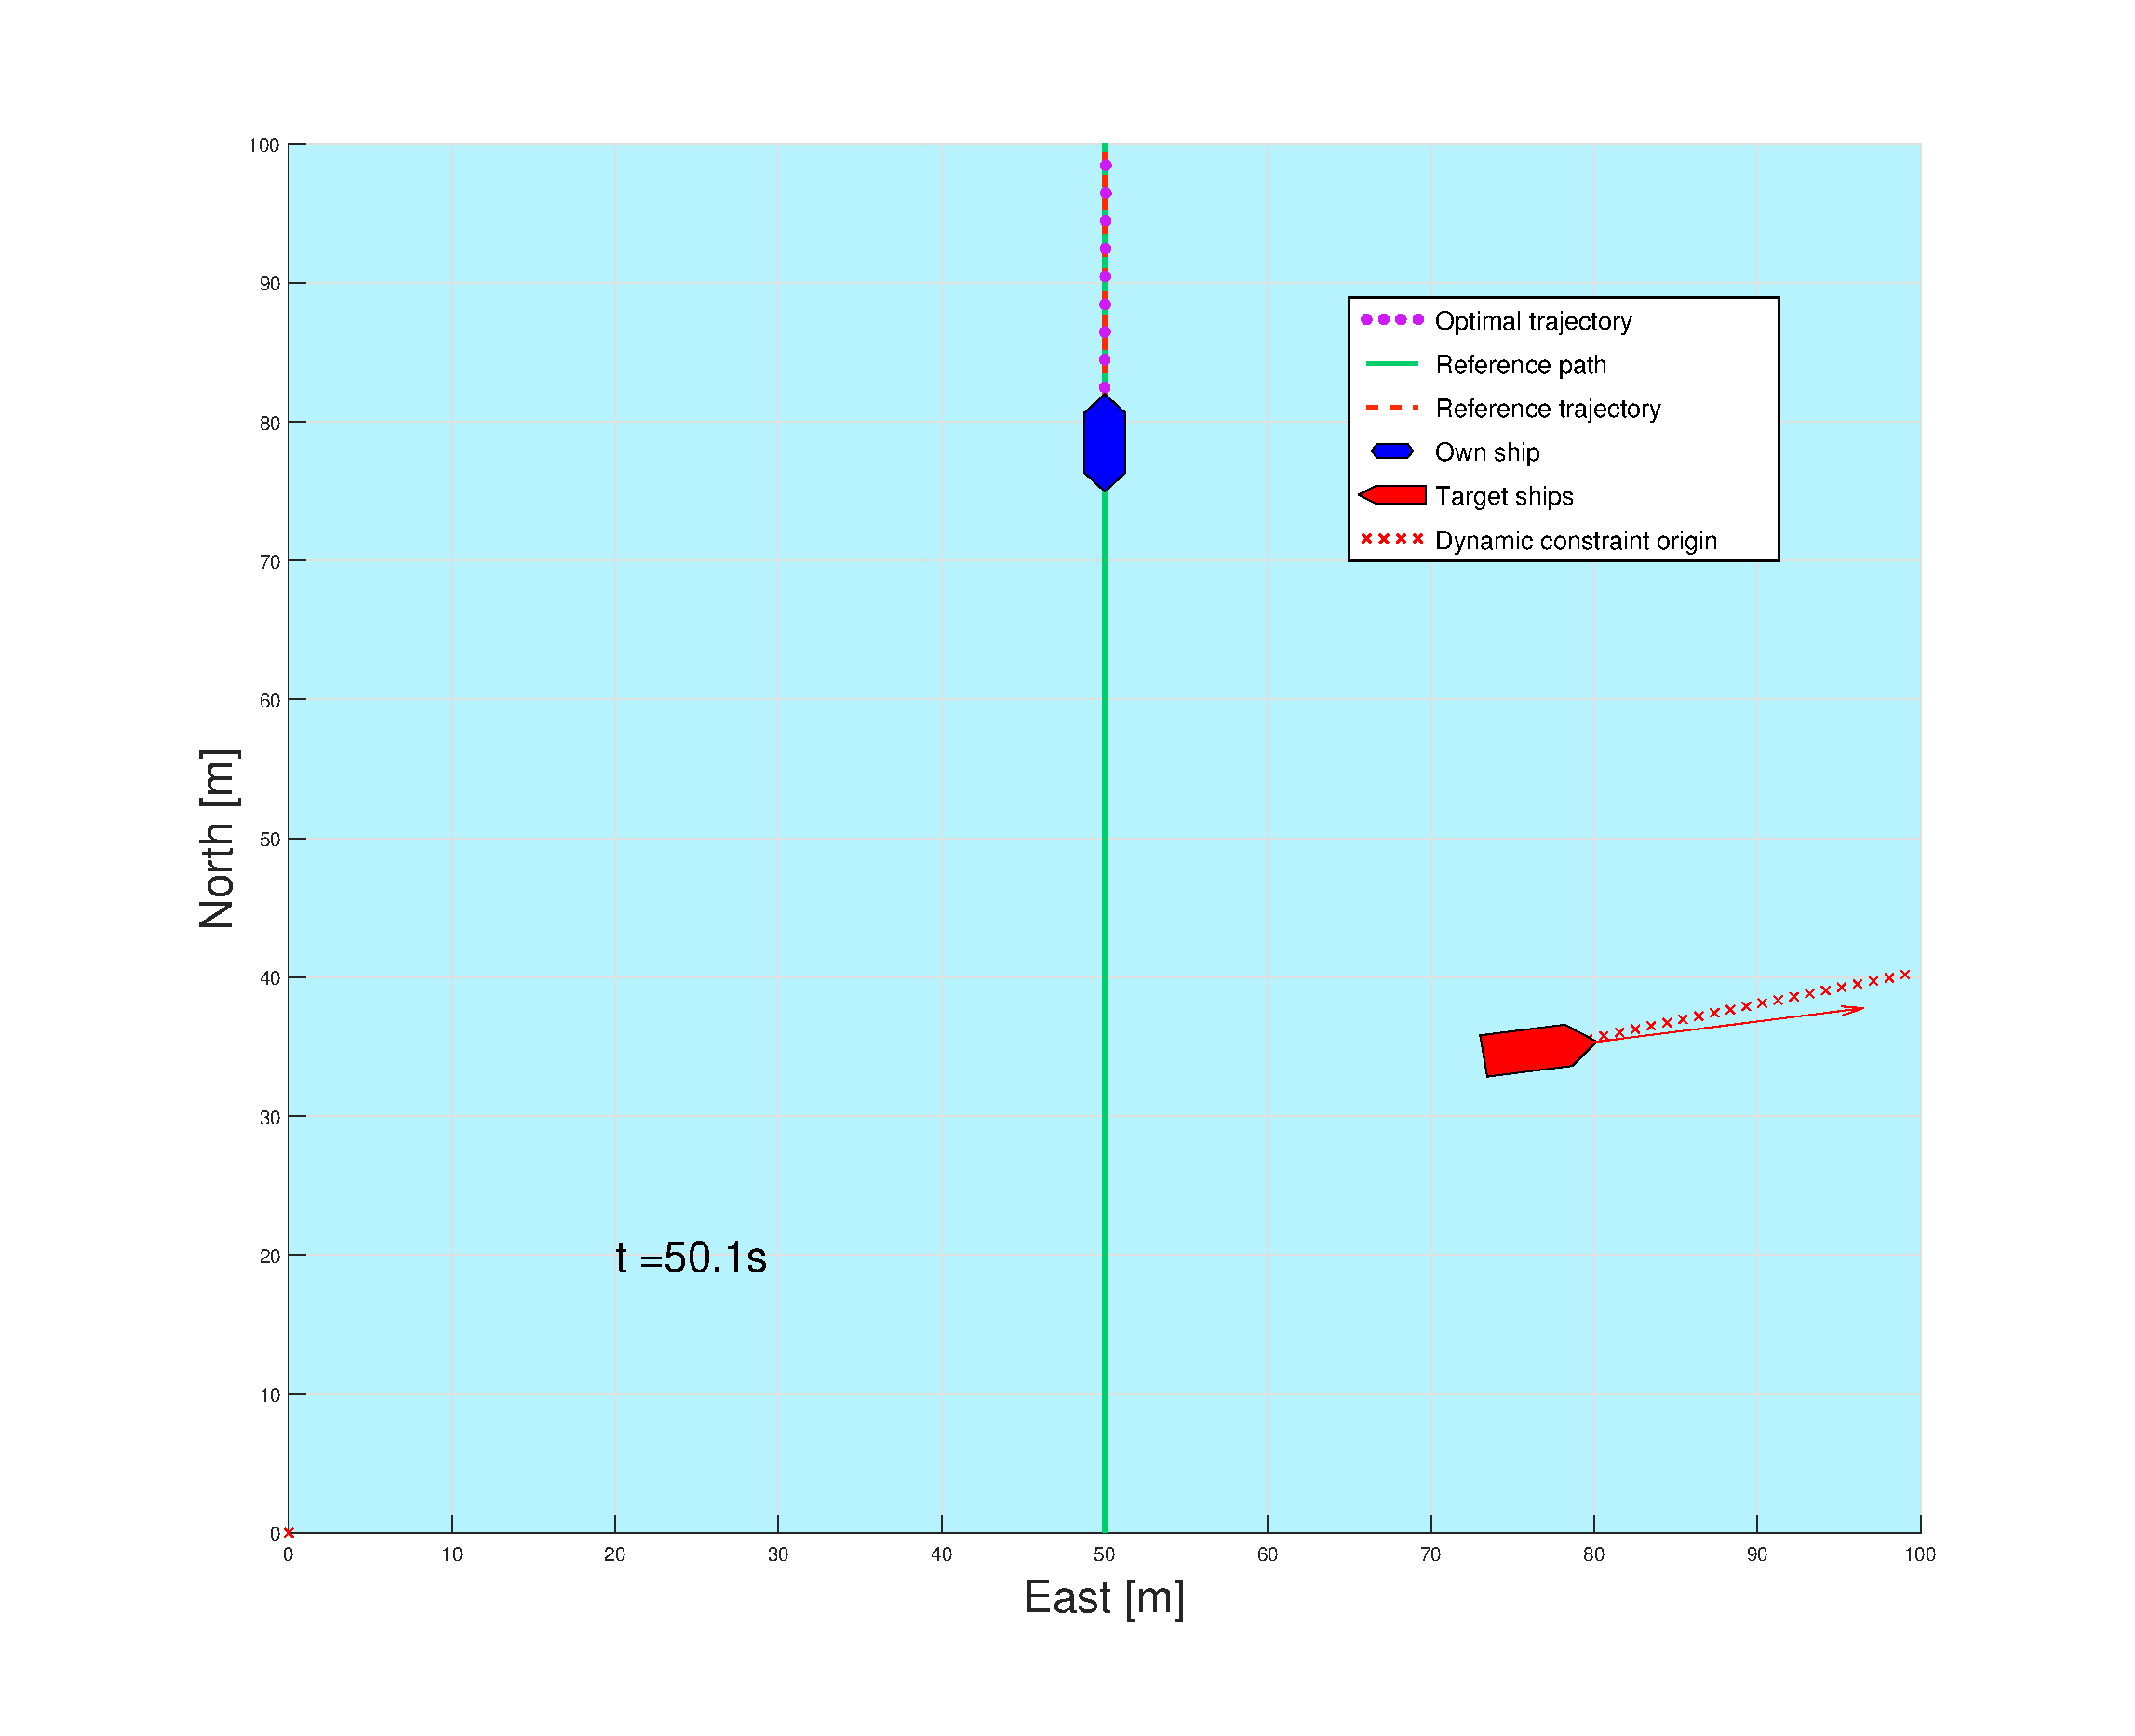
\includegraphics[width=\textwidth]{Images/Figures/enkel_SO/_Simple_0fig999_time=50}
        \subcaption{mhm}
    \end{subfigure}
    \hfill
    \\
    \begin{subfigure}[b]{0.49\textwidth}
        \centering
        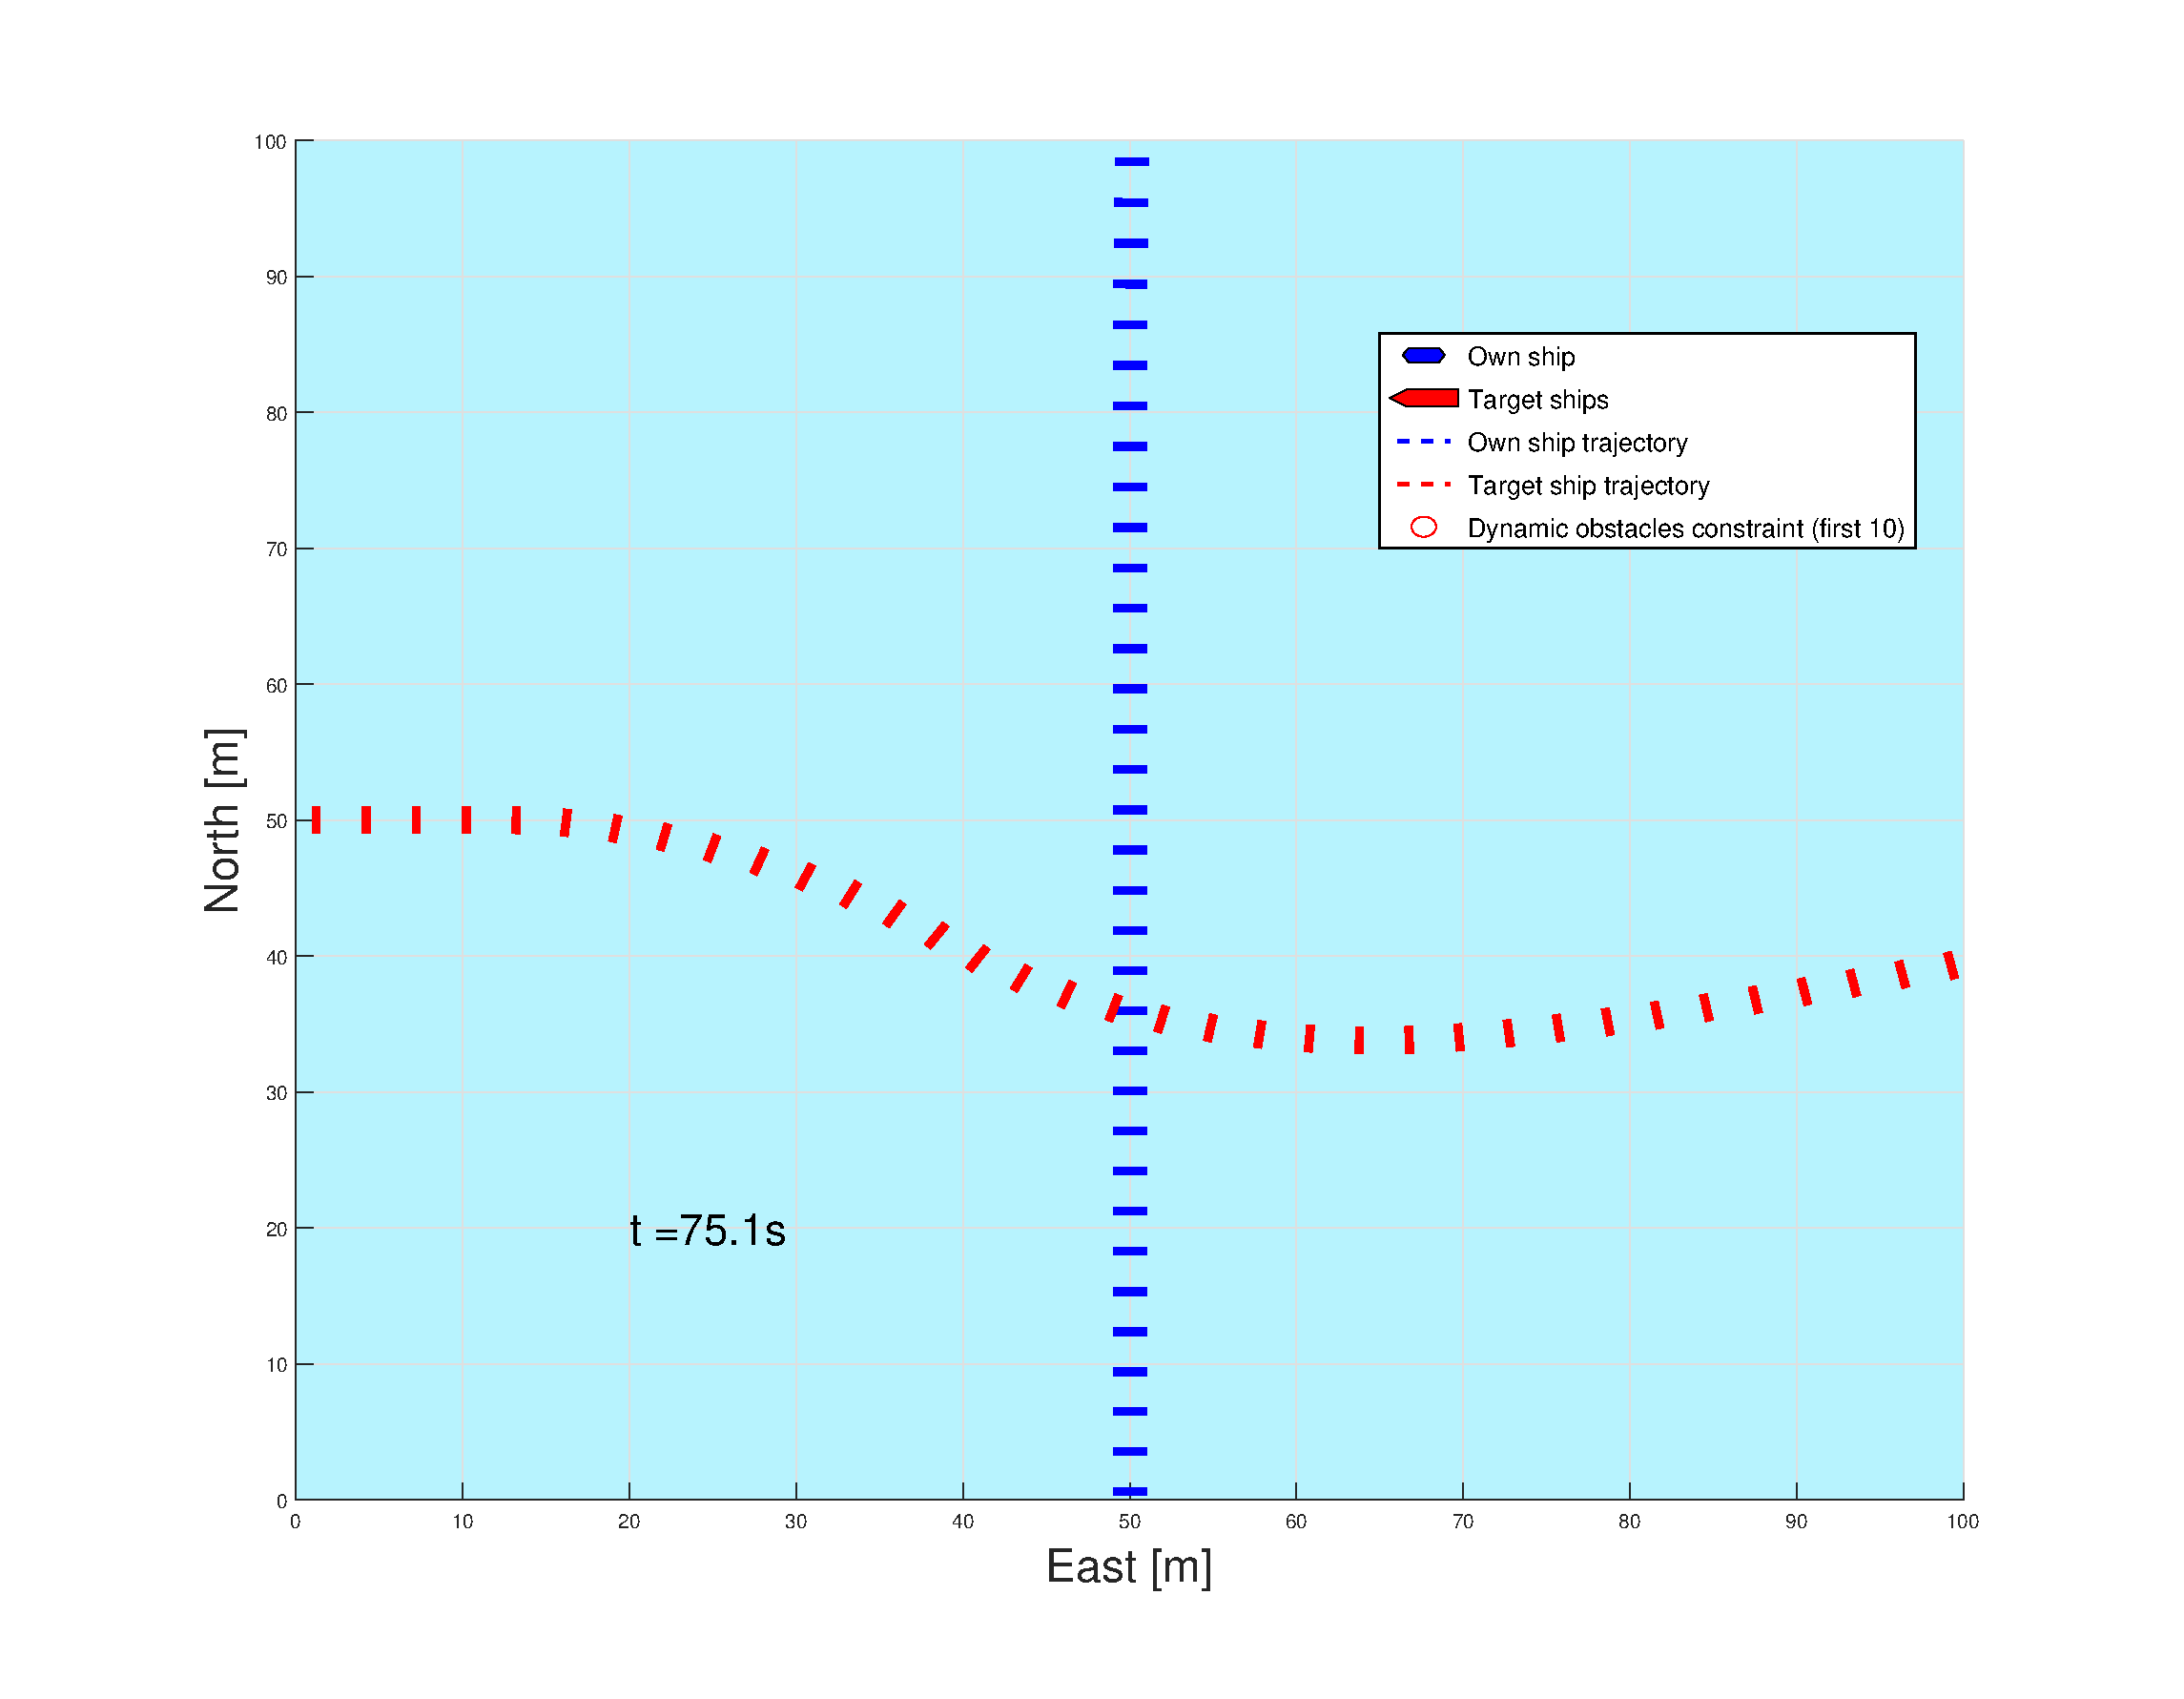
\includegraphics[width=\textwidth]{Images/Figures/enkel_SO/_Simple_0fig1_time=75}
        \subcaption{caption}
    \end{subfigure}
    \hfill
    \begin{subfigure}[b]{0.499\textwidth}
        \centering
        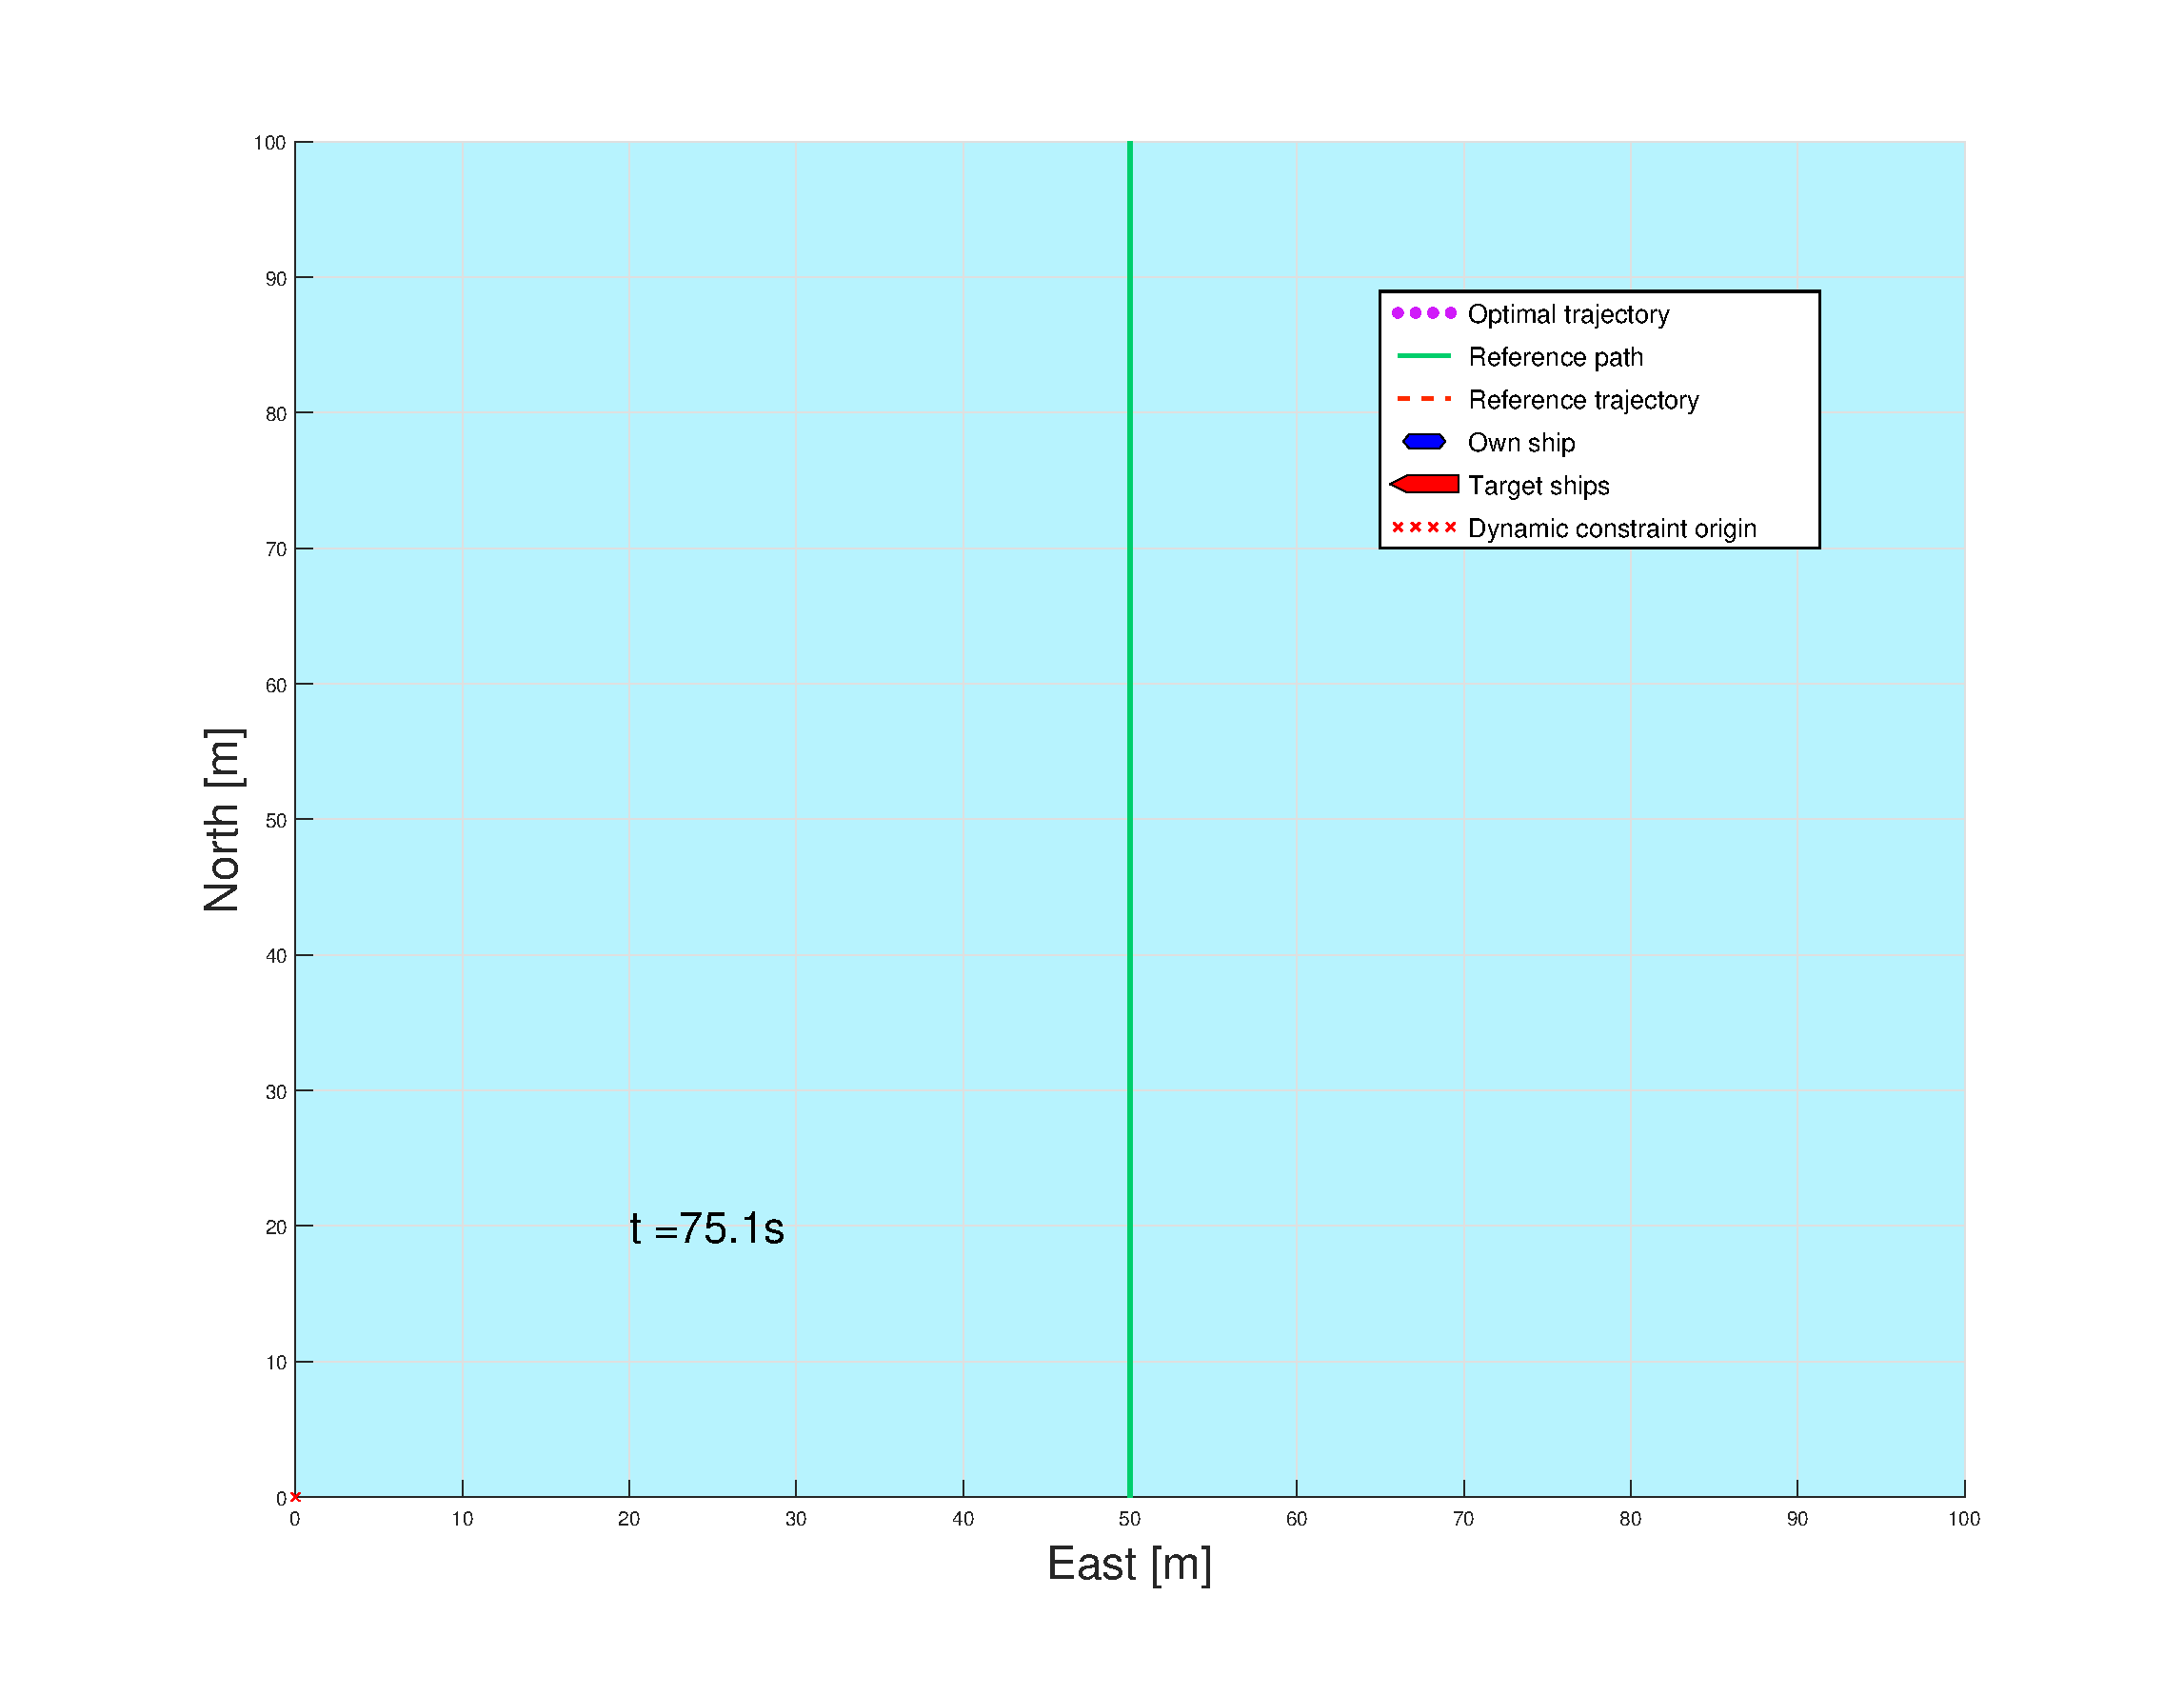
\includegraphics[width=\textwidth]{Images/Figures/enkel_SO/_Simple_0fig999_time=75}
        \subcaption{mhm}
    \end{subfigure}
    \hfill
    \caption{Simple Stand On With Prediction}
\end{figure}

\begin{figure}[!b] %Canals simulation, shown with and without constraints
    \begin{subfigure}[b]{0.49\textwidth}
        \centering
        \includegraphics[width=\textwidth]{Images/Figures/enkel_SO/_Simple_1fig1_time=0}
        \subcaption{caption}
    \end{subfigure}
    \hfill
    \begin{subfigure}[b]{0.499\textwidth}
        \centering
        \includegraphics[width=\textwidth]{Images/Figures/enkel_SO/_Simple_1fig999_time=0}
        \subcaption{mhm}
    \end{subfigure}
    \hfill
    \\
    \begin{subfigure}[b]{0.49\textwidth}
        \centering
        \includegraphics[width=\textwidth]{Images/Figures/enkel_SO/_Simple_1fig1_time=1}
        \subcaption{caption}
    \end{subfigure}
    \hfill
    \begin{subfigure}[b]{0.499\textwidth}
        \centering
        \includegraphics[width=\textwidth]{Images/Figures/enkel_SO/_Simple_1fig999_time=1}
        \subcaption{mhm}
    \end{subfigure}
    \hfill
    \\
    \begin{subfigure}[b]{0.49\textwidth}
        \centering
        \includegraphics[width=\textwidth]{Images/Figures/enkel_SO/_Simple_1fig1_time=25}
        \subcaption{caption}
    \end{subfigure}
    \hfill
    \begin{subfigure}[b]{0.499\textwidth}
        \centering
        \includegraphics[width=\textwidth]{Images/Figures/enkel_SO/_Simple_1fig999_time=25}
        \subcaption{mhm}
    \end{subfigure}
    \hfill
\end{figure}%
\begin{figure}[ht]\ContinuedFloat
    \begin{subfigure}[b]{0.49\textwidth}
        \centering
        \includegraphics[width=\textwidth]{Images/Figures/enkel_SO/_Simple_1fig1_time=50}
        \subcaption{caption}
    \end{subfigure}
    \hfill
    \begin{subfigure}[b]{0.499\textwidth}
        \centering
        \includegraphics[width=\textwidth]{Images/Figures/enkel_SO/_Simple_1fig999_time=50}
        \subcaption{mhm}
    \end{subfigure}
    \hfill
    \\
    \begin{subfigure}[b]{0.49\textwidth}
        \centering
        \includegraphics[width=\textwidth]{Images/Figures/enkel_SO/_Simple_1fig1_time=75}
        \subcaption{caption}
    \end{subfigure}
    \hfill
    \begin{subfigure}[b]{0.499\textwidth}
        \centering
        \includegraphics[width=\textwidth]{Images/Figures/enkel_SO/_Simple_1fig999_time=75}
        \subcaption{mhm}
    \end{subfigure}
    \hfill
    \caption{Simple Stand On Without Prediction}
\end{figure}

\subsubsection{Turn Head On}
\begin{itemize}
    \item THIS SCENARIO SHOULD BE MIRRORED HORIZONTALLY TO INCREASE THE CHANCES OF AN OBSERVABLE DIFFERENCE BETWEEN PREDICTIONS.
    \item otherwise business as usual, turns aren't predicted quite right.
\end{itemize}
\clearpage
\begin{figure}[!b] % TURN HEAD ON WITH PREDICTION
    \begin{subfigure}[b]{0.49\textwidth}
        \centering
        \includegraphics[width=\textwidth]{Images/Figures/sving_HO/_Simple_0fig1_time=1}
        \subcaption{caption}
    \end{subfigure}
    \hfill
    \begin{subfigure}[b]{0.499\textwidth}
        \centering
        \includegraphics[width=\textwidth]{Images/Figures/sving_HO/_Simple_0fig999_time=1}
        \subcaption{mhm}
    \end{subfigure}
    \hfill
    \\
    \begin{subfigure}[b]{0.49\textwidth}
        \centering
        \includegraphics[width=\textwidth]{Images/Figures/sving_HO/_Simple_0fig1_time=25}
        \subcaption{caption}
    \end{subfigure}
    \hfill
    \begin{subfigure}[b]{0.499\textwidth}
        \centering
        \includegraphics[width=\textwidth]{Images/Figures/sving_HO/_Simple_0fig999_time=25}
        \subcaption{mhm}
    \end{subfigure}
    \hfill
    \\
    \begin{subfigure}[b]{0.49\textwidth}
        \centering
        \includegraphics[width=\textwidth]{Images/Figures/sving_HO/_Simple_0fig1_time=50}
        \subcaption{caption}
    \end{subfigure}
    \hfill
    \begin{subfigure}[b]{0.499\textwidth}
        \centering
        \includegraphics[width=\textwidth]{Images/Figures/sving_HO/_Simple_0fig999_time=50}
        \subcaption{mhm}
    \end{subfigure}
    \hfill
\end{figure}%
\begin{figure}[ht]\ContinuedFloat
    \begin{subfigure}[b]{0.49\textwidth}
        \centering
        \includegraphics[width=\textwidth]{Images/Figures/sving_HO/_Simple_0fig1_time=75}
        \subcaption{caption}
    \end{subfigure}
    \hfill
    \begin{subfigure}[b]{0.499\textwidth}
        \centering
        \includegraphics[width=\textwidth]{Images/Figures/sving_HO/_Simple_0fig999_time=75}
        \subcaption{mhm}
    \end{subfigure}
    \hfill
    \\
    \begin{subfigure}[b]{0.49\textwidth}
        \centering
        \includegraphics[width=\textwidth]{Images/Figures/sving_HO/_Simple_0fig1_time=101}
        \subcaption{caption}
    \end{subfigure}
    \hfill
    \begin{subfigure}[b]{0.499\textwidth}
        \centering
        \includegraphics[width=\textwidth]{Images/Figures/sving_HO/_Simple_0fig999_time=101}
        \subcaption{mhm}
    \end{subfigure}
    \hfill
    \caption{Turn Head On With Prediction}
\end{figure}

\begin{figure}[!b] % TURN HEAD ON WITHOUT PREDICTION
    \begin{subfigure}[b]{0.49\textwidth}
        \centering
        \includegraphics[width=\textwidth]{Images/Figures/sving_HO/_Simple_1fig1_time=1}
        \subcaption{caption}
    \end{subfigure}
    \hfill
    \begin{subfigure}[b]{0.499\textwidth}
        \centering
        \includegraphics[width=\textwidth]{Images/Figures/sving_HO/_Simple_1fig999_time=1}
        \subcaption{mhm}
    \end{subfigure}
    \hfill
    \\
    \begin{subfigure}[b]{0.49\textwidth}
        \centering
        \includegraphics[width=\textwidth]{Images/Figures/sving_HO/_Simple_1fig1_time=25}
        \subcaption{caption}
    \end{subfigure}
    \hfill
    \begin{subfigure}[b]{0.499\textwidth}
        \centering
        \includegraphics[width=\textwidth]{Images/Figures/sving_HO/_Simple_1fig999_time=25}
        \subcaption{mhm}
    \end{subfigure}
    \hfill
    \\
    \begin{subfigure}[b]{0.49\textwidth}
        \centering
        \includegraphics[width=\textwidth]{Images/Figures/sving_HO/_Simple_1fig1_time=50}
        \subcaption{caption}
    \end{subfigure}
    \hfill
    \begin{subfigure}[b]{0.499\textwidth}
        \centering
        \includegraphics[width=\textwidth]{Images/Figures/sving_HO/_Simple_1fig999_time=50}
        \subcaption{mhm}
    \end{subfigure}
    \hfill
\end{figure}%
\begin{figure}[ht]\ContinuedFloat
    \begin{subfigure}[b]{0.49\textwidth}
        \centering
        \includegraphics[width=\textwidth]{Images/Figures/sving_HO/_Simple_1fig1_time=75}
        \subcaption{caption}
    \end{subfigure}
    \hfill
    \begin{subfigure}[b]{0.499\textwidth}
        \centering
        \includegraphics[width=\textwidth]{Images/Figures/sving_HO/_Simple_1fig999_time=75}
        \subcaption{mhm}
    \end{subfigure}
    \hfill
    \\
    \begin{subfigure}[b]{0.49\textwidth}
        \centering
        \includegraphics[width=\textwidth]{Images/Figures/sving_HO/_Simple_1fig1_time=101}
        \subcaption{caption}
    \end{subfigure}
    \hfill
    \begin{subfigure}[b]{0.499\textwidth}
        \centering
        \includegraphics[width=\textwidth]{Images/Figures/sving_HO/_Simple_1fig999_time=101}
        \subcaption{mhm}
    \end{subfigure}
    \hfill
    \caption{Turn Head On WithOUT Prediction}
\end{figure}

\subsubsection{Turn Give Way}
\begin{itemize}
    \item Here we finally observe a big differene between full and simple prediction.
    \item due to how the situation plays out the \gls{OS} is dragged along by the constraints of the \gls{Ts}.
    \item being dragged by constraints is not unique to this situation, and is one of the problems that can occur
    with this method of collision avoidance.
\end{itemize}

\clearpage
\begin{figure}[!b] % TURN GIVE WAY WITH PREDICTION
    \begin{subfigure}[b]{0.49\textwidth}
        \centering
        \includegraphics[width=\textwidth]{Images/Figures/sving_GW/_Simple_0fig1_time=1}
        \subcaption{caption}
    \end{subfigure}
    \hfill
    \begin{subfigure}[b]{0.499\textwidth}
        \centering
        \includegraphics[width=\textwidth]{Images/Figures/sving_GW/_Simple_0fig999_time=1}
        \subcaption{mhm}
    \end{subfigure}
    \hfill
    \\
    \begin{subfigure}[b]{0.49\textwidth}
        \centering
        \includegraphics[width=\textwidth]{Images/Figures/sving_GW/_Simple_0fig1_time=25}
        \subcaption{caption}
    \end{subfigure}
    \hfill
    \begin{subfigure}[b]{0.499\textwidth}
        \centering
        \includegraphics[width=\textwidth]{Images/Figures/sving_GW/_Simple_0fig999_time=25}
        \subcaption{mhm}
    \end{subfigure}
    \hfill
    \\
    \begin{subfigure}[b]{0.49\textwidth}
        \centering
        \includegraphics[width=\textwidth]{Images/Figures/sving_GW/_Simple_0fig1_time=50}
        \subcaption{caption}
    \end{subfigure}
    \hfill
    \begin{subfigure}[b]{0.499\textwidth}
        \centering
        \includegraphics[width=\textwidth]{Images/Figures/sving_GW/_Simple_0fig999_time=50}
        \subcaption{mhm}
    \end{subfigure}
    \hfill
\end{figure}%
\begin{figure}[ht]\ContinuedFloat
    \begin{subfigure}[b]{0.49\textwidth}
        \centering
        \includegraphics[width=\textwidth]{Images/Figures/sving_GW/_Simple_0fig1_time=75}
        \subcaption{caption}
    \end{subfigure}
    \hfill
    \begin{subfigure}[b]{0.499\textwidth}
        \centering
        \includegraphics[width=\textwidth]{Images/Figures/sving_GW/_Simple_0fig999_time=75}
        \subcaption{mhm}
    \end{subfigure}
    \hfill
    \\
    \begin{subfigure}[b]{0.49\textwidth}
        \centering
        \includegraphics[width=\textwidth]{Images/Figures/sving_GW/_Simple_0fig1_time=101}
        \subcaption{caption}
    \end{subfigure}
    \hfill
    \begin{subfigure}[b]{0.499\textwidth}
        \centering
        \includegraphics[width=\textwidth]{Images/Figures/sving_GW/_Simple_0fig999_time=101}
        \subcaption{mhm}
    \end{subfigure}
    \hfill
    \caption{Turn GIVE WAY With Prediction}
\end{figure}

\begin{figure}[!b] % TURN GIVE WAY ON WITHOUT PREDICTION
    \begin{subfigure}[b]{0.49\textwidth}
        \centering
        \includegraphics[width=\textwidth]{Images/Figures/sving_GW/_Simple_1fig1_time=1}
        \subcaption{caption}
    \end{subfigure}
    \hfill
    \begin{subfigure}[b]{0.499\textwidth}
        \centering
        \includegraphics[width=\textwidth]{Images/Figures/sving_GW/_Simple_1fig999_time=1}
        \subcaption{mhm}
    \end{subfigure}
    \hfill
    \\
    \begin{subfigure}[b]{0.49\textwidth}
        \centering
        \includegraphics[width=\textwidth]{Images/Figures/sving_GW/_Simple_1fig1_time=25}
        \subcaption{caption}
    \end{subfigure}
    \hfill
    \begin{subfigure}[b]{0.499\textwidth}
        \centering
        \includegraphics[width=\textwidth]{Images/Figures/sving_GW/_Simple_1fig999_time=25}
        \subcaption{mhm}
    \end{subfigure}
    \hfill
    \\
    \begin{subfigure}[b]{0.49\textwidth}
        \centering
        \includegraphics[width=\textwidth]{Images/Figures/sving_GW/_Simple_1fig1_time=50}
        \subcaption{caption}
    \end{subfigure}
    \hfill
    \begin{subfigure}[b]{0.499\textwidth}
        \centering
        \includegraphics[width=\textwidth]{Images/Figures/sving_GW/_Simple_1fig999_time=50}
        \subcaption{mhm}
    \end{subfigure}
    \hfill
\end{figure}%
\begin{figure}[ht]\ContinuedFloat
    \begin{subfigure}[b]{0.49\textwidth}
        \centering
        \includegraphics[width=\textwidth]{Images/Figures/sving_GW/_Simple_1fig1_time=75}
        \subcaption{caption}
    \end{subfigure}
    \hfill
    \begin{subfigure}[b]{0.499\textwidth}
        \centering
        \includegraphics[width=\textwidth]{Images/Figures/sving_GW/_Simple_1fig999_time=75}
        \subcaption{mhm}
    \end{subfigure}
    \hfill
    \\
    \begin{subfigure}[b]{0.49\textwidth}
        \centering
        \includegraphics[width=\textwidth]{Images/Figures/sving_GW/_Simple_1fig1_time=101}
        \subcaption{caption}
    \end{subfigure}
    \hfill
    \begin{subfigure}[b]{0.499\textwidth}
        \centering
        \includegraphics[width=\textwidth]{Images/Figures/sving_GW/_Simple_1fig999_time=101}
        \subcaption{mhm}
    \end{subfigure}
    \hfill
    \caption{Turn GIVE WAY WithOUT Prediction}
\end{figure}

\subsubsection{Turn Stand On}
\begin{itemize}
    \item Absolutely nothing happens here. move on.
\end{itemize}

\clearpage
\begin{figure}[!b] % TURN STAND ON WITH PREDICTION
    \begin{subfigure}[b]{0.49\textwidth}
        \centering
        \includegraphics[width=\textwidth]{Images/Figures/sving_SO/_Simple_0fig1_time=1}
        \subcaption{caption}
    \end{subfigure}
    \hfill
    \begin{subfigure}[b]{0.499\textwidth}
        \centering
        \includegraphics[width=\textwidth]{Images/Figures/sving_SO/_Simple_0fig999_time=1}
        \subcaption{mhm}
    \end{subfigure}
    \hfill
    \\
    \begin{subfigure}[b]{0.49\textwidth}
        \centering
        \includegraphics[width=\textwidth]{Images/Figures/sving_SO/_Simple_0fig1_time=25}
        \subcaption{caption}
    \end{subfigure}
    \hfill
    \begin{subfigure}[b]{0.499\textwidth}
        \centering
        \includegraphics[width=\textwidth]{Images/Figures/sving_SO/_Simple_0fig999_time=25}
        \subcaption{mhm}
    \end{subfigure}
    \hfill
    \\
    \begin{subfigure}[b]{0.49\textwidth}
        \centering
        \includegraphics[width=\textwidth]{Images/Figures/sving_SO/_Simple_0fig1_time=50}
        \subcaption{caption}
    \end{subfigure}
    \hfill
    \begin{subfigure}[b]{0.499\textwidth}
        \centering
        \includegraphics[width=\textwidth]{Images/Figures/sving_SO/_Simple_0fig999_time=50}
        \subcaption{mhm}
    \end{subfigure}
    \hfill
\end{figure}%
\begin{figure}[ht]\ContinuedFloat
    \begin{subfigure}[b]{0.49\textwidth}
        \centering
        \includegraphics[width=\textwidth]{Images/Figures/sving_SO/_Simple_0fig1_time=75}
        \subcaption{caption}
    \end{subfigure}
    \hfill
    \begin{subfigure}[b]{0.499\textwidth}
        \centering
        \includegraphics[width=\textwidth]{Images/Figures/sving_SO/_Simple_0fig999_time=75}
        \subcaption{mhm}
    \end{subfigure}
    \hfill
    \\
    \begin{subfigure}[b]{0.49\textwidth}
        \centering
        \includegraphics[width=\textwidth]{Images/Figures/sving_SO/_Simple_0fig1_time=101}
        \subcaption{caption}
    \end{subfigure}
    \hfill
    \begin{subfigure}[b]{0.499\textwidth}
        \centering
        \includegraphics[width=\textwidth]{Images/Figures/sving_SO/_Simple_0fig999_time=101}
        \subcaption{mhm}
    \end{subfigure}
    \hfill
    \caption{Turn Stand On With Prediction}
\end{figure}

\begin{figure}[!b] % TURN STAND ON WITHOUT PREDICTION
    \begin{subfigure}[b]{0.49\textwidth}
        \centering
        \includegraphics[width=\textwidth]{Images/Figures/sving_SO/_Simple_1fig1_time=1}
        \subcaption{caption}
    \end{subfigure}
    \hfill
    \begin{subfigure}[b]{0.499\textwidth}
        \centering
        \includegraphics[width=\textwidth]{Images/Figures/sving_SO/_Simple_1fig999_time=1}
        \subcaption{mhm}
    \end{subfigure}
    \hfill
    \\
    \begin{subfigure}[b]{0.49\textwidth}
        \centering
        \includegraphics[width=\textwidth]{Images/Figures/sving_SO/_Simple_1fig1_time=25}
        \subcaption{caption}
    \end{subfigure}
    \hfill
    \begin{subfigure}[b]{0.499\textwidth}
        \centering
        \includegraphics[width=\textwidth]{Images/Figures/sving_SO/_Simple_1fig999_time=25}
        \subcaption{mhm}
    \end{subfigure}
    \hfill
    \\
    \begin{subfigure}[b]{0.49\textwidth}
        \centering
        \includegraphics[width=\textwidth]{Images/Figures/sving_SO/_Simple_1fig1_time=50}
        \subcaption{caption}
    \end{subfigure}
    \hfill
    \begin{subfigure}[b]{0.499\textwidth}
        \centering
        \includegraphics[width=\textwidth]{Images/Figures/sving_SO/_Simple_1fig999_time=50}
        \subcaption{mhm}
    \end{subfigure}
    \hfill
\end{figure}%
\begin{figure}[ht]\ContinuedFloat
    \begin{subfigure}[b]{0.49\textwidth}
        \centering
        \includegraphics[width=\textwidth]{Images/Figures/sving_SO/_Simple_1fig1_time=75}
        \subcaption{caption}
    \end{subfigure}
    \hfill
    \begin{subfigure}[b]{0.499\textwidth}
        \centering
        \includegraphics[width=\textwidth]{Images/Figures/sving_SO/_Simple_1fig999_time=75}
        \subcaption{mhm}
    \end{subfigure}
    \hfill
    \\
    \begin{subfigure}[b]{0.49\textwidth}
        \centering
        \includegraphics[width=\textwidth]{Images/Figures/sving_SO/_Simple_1fig1_time=101}
        \subcaption{caption}
    \end{subfigure}
    \hfill
    \begin{subfigure}[b]{0.499\textwidth}
        \centering
        \includegraphics[width=\textwidth]{Images/Figures/sving_SO/_Simple_1fig999_time=101}
        \subcaption{mhm}
    \end{subfigure}
    \hfill
    \caption{Turn Stand On WithOUT Prediction}
\end{figure}

\subsubsection{Canals}
\begin{itemize}
    \item blocked path
    \item feasibility check
    \item forskjell mellom prediction metoder
    % \item not entirely clear to me which behaviour is the most 'COLREGs compliant'
    \item When the path is blocked it takes a very very very long time to solve the NLP, users beware.
    \item Get to see static obstacles in effect.
\end{itemize}

\clearpage
\begin{figure}[!b] %Canals simulation, shown with and without constraints
    \begin{subfigure}[b]{0.49\textwidth}
        \centering
        \includegraphics[width=\textwidth]{Images/Figures/Havn1/_Simple_0fig1_time=0}
        \subcaption{caption}
    \end{subfigure}
    \hfill
    \begin{subfigure}[b]{0.499\textwidth}
        \centering
        \includegraphics[width=\textwidth]{Images/Figures/Havn1/_Simple_0fig999_time=0}
        \subcaption{mhm}
    \end{subfigure}
    \hfill
    \\
    \begin{subfigure}[b]{0.49\textwidth}
        \centering
        \includegraphics[width=\textwidth]{Images/Figures/Havn1/_Simple_0fig1_time=1}
        \subcaption{caption}
    \end{subfigure}
    \hfill
    \begin{subfigure}[b]{0.499\textwidth}
        \centering
        \includegraphics[width=\textwidth]{Images/Figures/Havn1/_Simple_0fig999_time=1}
        \subcaption{mhm}
    \end{subfigure}
    \hfill
    \\
    \begin{subfigure}[b]{0.49\textwidth}
        \centering
        \includegraphics[width=\textwidth]{Images/Figures/Havn1/_Simple_0fig1_time=25}
        \subcaption{caption}
    \end{subfigure}
    \hfill
    \begin{subfigure}[b]{0.499\textwidth}
        \centering
        \includegraphics[width=\textwidth]{Images/Figures/Havn1/_Simple_0fig999_time=25}
        \subcaption{mhm}
    \end{subfigure}
    \hfill
\end{figure}%
\begin{figure}[ht]\ContinuedFloat
    \begin{subfigure}[b]{0.49\textwidth}
        \centering
        \includegraphics[width=\textwidth]{Images/Figures/Havn1/_Simple_0fig1_time=50}
        \subcaption{caption}
    \end{subfigure}
    \hfill
    \begin{subfigure}[b]{0.499\textwidth}
        \centering
        \includegraphics[width=\textwidth]{Images/Figures/Havn1/_Simple_0fig999_time=50}
        \subcaption{mhm}
    \end{subfigure}
    \hfill
    \\
    \begin{subfigure}[b]{0.49\textwidth}
        \centering
        \includegraphics[width=\textwidth]{Images/Figures/Havn1/_Simple_0fig1_time=75}
        \subcaption{caption}
    \end{subfigure}
    \hfill
    \begin{subfigure}[b]{0.499\textwidth}
        \centering
        \includegraphics[width=\textwidth]{Images/Figures/Havn1/_Simple_0fig999_time=75}
        \subcaption{mhm}
    \end{subfigure}
    \hfill
    \\ 
    \begin{subfigure}[b]{0.49\textwidth}
        \centering
        \includegraphics[width=\textwidth]{Images/Figures/Havn1/_Simple_0fig1_time=101}
        \subcaption{caption}
    \end{subfigure}
    \hfill
    \begin{subfigure}[b]{0.499\textwidth}
        \centering
        \includegraphics[width=\textwidth]{Images/Figures/Havn1/_Simple_0fig999_time=101}
        \subcaption{mhm}
    \end{subfigure}
    \hfill
\end{figure}
\begin{figure}[ht]\ContinuedFloat
    \begin{subfigure}[b]{0.49\textwidth}
        \centering
        \includegraphics[width=\textwidth]{Images/Figures/Havn1/_Simple_0fig1_time=126}
        \subcaption{caption}
    \end{subfigure}
    \hfill
    \begin{subfigure}[b]{0.499\textwidth}
        \centering
        \includegraphics[width=\textwidth]{Images/Figures/Havn1/_Simple_0fig999_time=126}
        \subcaption{mhm}
    \end{subfigure}
    \hfill
    \caption{Canals simulation. On the left shown with current active dynamic and static constraints. On the right seen with projected future trajectory}
\end{figure}

\clearpage
\begin{figure}[!b] %Canals simulation without prediction, shown with and without constraints
    \begin{subfigure}[b]{0.49\textwidth}
        \centering
        \includegraphics[width=\textwidth]{Images/Figures/Havn1/_Simple_1fig1_time=0}
        \caption{caption}
    \end{subfigure}
    \hfill
    \begin{subfigure}[b]{0.499\textwidth}
        \centering
        \includegraphics[width=\textwidth]{Images/Figures/Havn1/_Simple_1fig999_time=0}
        \caption{mhm}
    \end{subfigure}
    \hfill
    \\
    \begin{subfigure}[b]{0.49\textwidth}
        \centering
        \includegraphics[width=\textwidth]{Images/Figures/Havn1/_Simple_1fig1_time=1}
        \caption{caption}
    \end{subfigure}
    \hfill
    \begin{subfigure}[b]{0.499\textwidth}
        \centering
        \includegraphics[width=\textwidth]{Images/Figures/Havn1/_Simple_1fig999_time=1}
        \caption{mhm}
    \end{subfigure}
    \hfill
    \\
    \begin{subfigure}[b]{0.49\textwidth}
        \centering
        \includegraphics[width=\textwidth]{Images/Figures/Havn1/_Simple_1fig1_time=25}
        \caption{caption}
    \end{subfigure}
    \hfill
    \begin{subfigure}[b]{0.499\textwidth}
        \centering
        \includegraphics[width=\textwidth]{Images/Figures/Havn1/_Simple_1fig999_time=25}
        \caption{mhm}
    \end{subfigure}
    \hfill
\end{figure}%
\begin{figure}[ht]\ContinuedFloat
    \begin{subfigure}[b]{0.49\textwidth}
        \centering
        \includegraphics[width=\textwidth]{Images/Figures/Havn1/_Simple_1fig1_time=50}
        \subcaption{dsadada}
    \end{subfigure}
    \hfill
    \begin{subfigure}[b]{0.499\textwidth}
        \centering
        \includegraphics[width=\textwidth]{Images/Figures/Havn1/_Simple_1fig999_time=50}
        \subcaption{mhm}
    \end{subfigure}
    \hfill
    \\
    \begin{subfigure}[b]{0.49\textwidth}
        \centering
        \includegraphics[width=\textwidth]{Images/Figures/Havn1/_Simple_1fig1_time=75}
        \subcaption{caption}
    \end{subfigure}
    \hfill
    \begin{subfigure}[b]{0.499\textwidth}
        \centering
        \includegraphics[width=\textwidth]{Images/Figures/Havn1/_Simple_1fig999_time=75}
        \subcaption{mhm}
    \end{subfigure}
    \hfill
    \\
    \begin{subfigure}[b]{0.49\textwidth}
        \centering
        \includegraphics[width=\textwidth]{Images/Figures/Havn1/_Simple_1fig1_time=101}
        \subcaption{caption}
    \end{subfigure}
    \hfill
    \begin{subfigure}[b]{0.499\textwidth}
        \centering
        \includegraphics[width=\textwidth]{Images/Figures/Havn1/_Simple_1fig999_time=101}
        \subcaption{mhm}
    \end{subfigure}
    \hfill
    \caption{Canals simulation without prediction, shown with and without constraints}
\end{figure}
\begin{figure}[ht]\ContinuedFloat
    \begin{subfigure}[b]{0.49\textwidth}
        \centering
        \includegraphics[width=\textwidth]{Images/Figures/Havn1/_Simple_1fig1_time=126}
        \subcaption{caption}
    \end{subfigure}
    \hfill
    \begin{subfigure}[b]{0.499\textwidth}
        \centering
        \includegraphics[width=\textwidth]{Images/Figures/Havn1/_Simple_1fig999_time=126}
        \subcaption{mhm}
    \end{subfigure}
    \hfill
    \caption{TODO: skriv. Havn1 w\_opt without prediction}
\end{figure}

\iffalse
Scenario der det er en statisk hindring midt i referanse banen.
Scenario der vi mer tydelig blir 'dyttet' inn mot statisk hindring av annen båt.
Scenario der det er overlap mellom forskjellige COLREGs situasjoner
Scenario med flere båter i samme COLREGs situasion, kan kombineres med scenario over.
Skjaergård MÅ inkludere en bane gjennom masse små skjær, ikke fordi det er vanlig men fordi det må testes.
\fi


\subsubsection{Trondheimsfjord}
\begin{itemize}
    \item COLREGs stress test
    \item Full prediction behaves much 'calmer', which is better in the author's opinion.
    \item Full prediction is also much more computationally efficient, for reasons that will be discussed later.
\end{itemize}
\clearpage
\begin{figure}[!b] %TRONDHEIMFJORD, WITH PREDICTION
    \begin{subfigure}[b]{0.49\textwidth}
        \centering
        \includegraphics[width=\textwidth]{Images/Figures/Trheimfjord/_Simple_0fig1_time=101}
        \subcaption{caption}
    \end{subfigure}
    \hfill
    \begin{subfigure}[b]{0.499\textwidth}
        \centering
        \includegraphics[width=\textwidth]{Images/Figures/Trheimfjord/_Simple_0fig999_time=101}
        \subcaption{mhm}
    \end{subfigure}
    \hfill
    \\
    \begin{subfigure}[b]{0.49\textwidth}
        \centering
        \includegraphics[width=\textwidth]{Images/Figures/Trheimfjord/_Simple_0fig1_time=126}
        \subcaption{caption}
    \end{subfigure}
    \hfill
    \begin{subfigure}[b]{0.499\textwidth}
        \centering
        \includegraphics[width=\textwidth]{Images/Figures/Trheimfjord/_Simple_0fig999_time=126}
        \subcaption{mhm}
    \end{subfigure}
    \hfill
    \\
    \begin{subfigure}[b]{0.49\textwidth}
        \centering
        \includegraphics[width=\textwidth]{Images/Figures/Trheimfjord/_Simple_0fig1_time=151}
        \subcaption{caption}
    \end{subfigure}
    \hfill
    \begin{subfigure}[b]{0.499\textwidth}
        \centering
        \includegraphics[width=\textwidth]{Images/Figures/Trheimfjord/_Simple_0fig999_time=151}
        \subcaption{mhm}
    \end{subfigure}
    \hfill
\end{figure}%
\begin{figure}[ht]\ContinuedFloat
    \begin{subfigure}[b]{0.49\textwidth}
        \centering
        \includegraphics[width=\textwidth]{Images/Figures/Trheimfjord/_Simple_0fig1_time=226}
        \subcaption{caption}
    \end{subfigure}
    \hfill
    \begin{subfigure}[b]{0.499\textwidth}
        \centering
        \includegraphics[width=\textwidth]{Images/Figures/Trheimfjord/_Simple_0fig999_time=226}
        \subcaption{mhm}
    \end{subfigure}
    \hfill
    \\
    \begin{subfigure}[b]{0.49\textwidth}
        \centering
        \includegraphics[width=\textwidth]{Images/Figures/Trheimfjord/_Simple_0fig1_time=251}
        \subcaption{caption}
    \end{subfigure}
    \hfill
    \begin{subfigure}[b]{0.499\textwidth}
        \centering
        \includegraphics[width=\textwidth]{Images/Figures/Trheimfjord/_Simple_0fig999_time=251}
        \subcaption{mhm}
    \end{subfigure}
    \hfill
    \\ 
    \begin{subfigure}[b]{0.49\textwidth}
        \centering
        \includegraphics[width=\textwidth]{Images/Figures/Trheimfjord/_Simple_0fig1_time=276}
        \subcaption{caption}
    \end{subfigure}
    \hfill
    \begin{subfigure}[b]{0.499\textwidth}
        \centering
        \includegraphics[width=\textwidth]{Images/Figures/Trheimfjord/_Simple_0fig999_time=276}
        \subcaption{mhm}
    \end{subfigure}
    \hfill
\end{figure}
\begin{figure}[ht]\ContinuedFloat
    \begin{subfigure}[b]{0.49\textwidth}
        \centering
        \includegraphics[width=\textwidth]{Images/Figures/Trheimfjord/_Simple_0fig1_time=301}
        \subcaption{caption}
    \end{subfigure}
    \hfill
    \begin{subfigure}[b]{0.499\textwidth}
        \centering
        \includegraphics[width=\textwidth]{Images/Figures/Trheimfjord/_Simple_0fig999_time=301}
        \subcaption{mhm}
    \end{subfigure}
    \hfill
    \\
    \begin{subfigure}[b]{0.49\textwidth}
        \centering
        \includegraphics[width=\textwidth]{Images/Figures/Trheimfjord/_Simple_0fig1_time=325}
        \subcaption{caption}
    \end{subfigure}
    \hfill
    \begin{subfigure}[b]{0.499\textwidth}
        \centering
        \includegraphics[width=\textwidth]{Images/Figures/Trheimfjord/_Simple_0fig999_time=325}
        \subcaption{mhm}
    \end{subfigure}
    \hfill
    \\
    \begin{subfigure}[b]{0.49\textwidth}
        \centering
        \includegraphics[width=\textwidth]{Images/Figures/Trheimfjord/_Simple_0fig1_time=350}
        \subcaption{caption}
    \end{subfigure}
    \hfill
    \begin{subfigure}[b]{0.499\textwidth}
        \centering
        \includegraphics[width=\textwidth]{Images/Figures/Trheimfjord/_Simple_0fig999_time=350}
        \subcaption{mhm}
    \end{subfigure}
    \hfill
    \caption{Trondheimfjord simulation. On the left shown with current active dynamic and static constraints. On the right seen with projected future trajectory}
\end{figure}


\clearpage
\begin{figure}[!b] %TRONDHEIMFJORD, WITHOUT PREDICTION
    \begin{subfigure}[b]{0.49\textwidth}
        \centering
        \includegraphics[width=\textwidth]{Images/Figures/Trheimfjord/_Simple_1fig1_time=101}
        \subcaption{caption}
    \end{subfigure}
    \hfill
    \begin{subfigure}[b]{0.499\textwidth}
        \centering
        \includegraphics[width=\textwidth]{Images/Figures/Trheimfjord/_Simple_1fig999_time=101}
        \subcaption{mhm}
    \end{subfigure}
    \hfill
    \\
    \begin{subfigure}[b]{0.49\textwidth}
        \centering
        \includegraphics[width=\textwidth]{Images/Figures/Trheimfjord/_Simple_1fig1_time=126}
        \subcaption{caption}
    \end{subfigure}
    \hfill
    \begin{subfigure}[b]{0.499\textwidth}
        \centering
        \includegraphics[width=\textwidth]{Images/Figures/Trheimfjord/_Simple_1fig999_time=126}
        \subcaption{mhm}
    \end{subfigure}
    \hfill
    \\
    \begin{subfigure}[b]{0.49\textwidth}
        \centering
        \includegraphics[width=\textwidth]{Images/Figures/Trheimfjord/_Simple_1fig1_time=151}
        \subcaption{caption}
    \end{subfigure}
    \hfill
    \begin{subfigure}[b]{0.499\textwidth}
        \centering
        \includegraphics[width=\textwidth]{Images/Figures/Trheimfjord/_Simple_1fig999_time=151}
        \subcaption{mhm}
    \end{subfigure}
    \hfill
\end{figure}%
\begin{figure}[ht]\ContinuedFloat
    \begin{subfigure}[b]{0.49\textwidth}
        \centering
        \includegraphics[width=\textwidth]{Images/Figures/Trheimfjord/_Simple_1fig1_time=226}
        \subcaption{caption}
    \end{subfigure}
    \hfill
    \begin{subfigure}[b]{0.499\textwidth}
        \centering
        \includegraphics[width=\textwidth]{Images/Figures/Trheimfjord/_Simple_1fig999_time=226}
        \subcaption{mhm}
    \end{subfigure}
    \hfill
    \\
    \begin{subfigure}[b]{0.49\textwidth}
        \centering
        \includegraphics[width=\textwidth]{Images/Figures/Trheimfjord/_Simple_1fig1_time=251}
        \subcaption{caption}
    \end{subfigure}
    \hfill
    \begin{subfigure}[b]{0.499\textwidth}
        \centering
        \includegraphics[width=\textwidth]{Images/Figures/Trheimfjord/_Simple_1fig999_time=251}
        \subcaption{mhm}
    \end{subfigure}
    \hfill
    \\ 
    \begin{subfigure}[b]{0.49\textwidth}
        \centering
        \includegraphics[width=\textwidth]{Images/Figures/Trheimfjord/_Simple_1fig1_time=276}
        \subcaption{caption}
    \end{subfigure}
    \hfill
    \begin{subfigure}[b]{0.499\textwidth}
        \centering
        \includegraphics[width=\textwidth]{Images/Figures/Trheimfjord/_Simple_1fig999_time=276}
        \subcaption{mhm}
    \end{subfigure}
    \hfill
\end{figure}
\begin{figure}[ht]\ContinuedFloat
    \begin{subfigure}[b]{0.49\textwidth}
        \centering
        \includegraphics[width=\textwidth]{Images/Figures/Trheimfjord/_Simple_1fig1_time=301}
        \subcaption{caption}
    \end{subfigure}
    \hfill
    \begin{subfigure}[b]{0.499\textwidth}
        \centering
        \includegraphics[width=\textwidth]{Images/Figures/Trheimfjord/_Simple_1fig999_time=301}
        \subcaption{mhm}
    \end{subfigure}
    \hfill
    \\
    \begin{subfigure}[b]{0.49\textwidth}
        \centering
        \includegraphics[width=\textwidth]{Images/Figures/Trheimfjord/_Simple_1fig1_time=325}
        \subcaption{caption}
    \end{subfigure}
    \hfill
    \begin{subfigure}[b]{0.499\textwidth}
        \centering
        \includegraphics[width=\textwidth]{Images/Figures/Trheimfjord/_Simple_1fig999_time=325}
        \subcaption{mhm}
    \end{subfigure}
    \hfill
    \\
    \begin{subfigure}[b]{0.49\textwidth}
        \centering
        \includegraphics[width=\textwidth]{Images/Figures/Trheimfjord/_Simple_1fig1_time=350}
        \subcaption{caption}
    \end{subfigure}
    \hfill
    \begin{subfigure}[b]{0.499\textwidth}
        \centering
        \includegraphics[width=\textwidth]{Images/Figures/Trheimfjord/_Simple_1fig999_time=350}
        \subcaption{mhm}
    \end{subfigure}
    \hfill
    \caption{Trondheimfjord simulation. On the left shown with current active dynamic and static constraints. On the right seen with projected future trajectory}
\end{figure}




\subsubsection{Helløya}
\begin{itemize}
    \item Both simple and full prediction actually navigate the 'invisible' turn quite well
    \item even in the reverse direction it's not really a problem, though simple prediction cuts the turn, which could be considered bad.
    \item when being overtaken the full prediction exhibits much better behaviour.
    \item This is one of the scenarios where the scale is very exaggerated.
\end{itemize}
(TODO: Skriv og figurer)
\clearpage
\begin{figure}[!b] %HELLOYA NORMAL, WITH PREDICTION
    \begin{subfigure}[b]{0.49\textwidth}
        \centering
        \includegraphics[width=\textwidth]{Images/Figures/Helloya/_Simple_0fig1_time=1}
        \subcaption{caption}
    \end{subfigure}
    \hfill
    \begin{subfigure}[b]{0.499\textwidth}
        \centering
        \includegraphics[width=\textwidth]{Images/Figures/Helloya/_Simple_0fig999_time=1}
        \subcaption{mhm}
    \end{subfigure}
    \hfill
    \\
    \begin{subfigure}[b]{0.49\textwidth}
        \centering
        \includegraphics[width=\textwidth]{Images/Figures/Helloya/_Simple_0fig1_time=25}
        \subcaption{caption}
    \end{subfigure}
    \hfill
    \begin{subfigure}[b]{0.499\textwidth}
        \centering
        \includegraphics[width=\textwidth]{Images/Figures/Helloya/_Simple_0fig999_time=25}
        \subcaption{mhm}
    \end{subfigure}
    \hfill
    \\
    \begin{subfigure}[b]{0.49\textwidth}
        \centering
        \includegraphics[width=\textwidth]{Images/Figures/Helloya/_Simple_0fig1_time=75}
        \subcaption{caption}
    \end{subfigure}
    \hfill
    \begin{subfigure}[b]{0.499\textwidth}
        \centering
        \includegraphics[width=\textwidth]{Images/Figures/Helloya/_Simple_0fig999_time=75}
        \subcaption{mhm}
    \end{subfigure}
    \hfill
\end{figure}%
\begin{figure}[ht]\ContinuedFloat
    \begin{subfigure}[b]{0.49\textwidth}
        \centering
        \includegraphics[width=\textwidth]{Images/Figures/Helloya/_Simple_0fig1_time=101}
        \subcaption{caption}
    \end{subfigure}
    \hfill
    \begin{subfigure}[b]{0.499\textwidth}
        \centering
        \includegraphics[width=\textwidth]{Images/Figures/Helloya/_Simple_0fig999_time=101}
        \subcaption{mhm}
    \end{subfigure}
    \hfill
    \\
    \begin{subfigure}[b]{0.49\textwidth}
        \centering
        \includegraphics[width=\textwidth]{Images/Figures/Helloya/_Simple_0fig1_time=126}
        \subcaption{caption}
    \end{subfigure}
    \hfill
    \begin{subfigure}[b]{0.499\textwidth}
        \centering
        \includegraphics[width=\textwidth]{Images/Figures/Helloya/_Simple_0fig999_time=126}
        \subcaption{mhm}
    \end{subfigure}
    \hfill
    \\ 
    \begin{subfigure}[b]{0.49\textwidth}
        \centering
        \includegraphics[width=\textwidth]{Images/Figures/Helloya/_Simple_0fig1_time=151}
        \subcaption{caption}
    \end{subfigure}
    \hfill
    \begin{subfigure}[b]{0.499\textwidth}
        \centering
        \includegraphics[width=\textwidth]{Images/Figures/Helloya/_Simple_0fig999_time=151}
        \subcaption{mhm}
    \end{subfigure}
    \hfill
\end{figure}
\begin{figure}[ht]\ContinuedFloat
    \begin{subfigure}[b]{0.49\textwidth}
        \centering
        \includegraphics[width=\textwidth]{Images/Figures/Helloya/_Simple_0fig1_time=176}
        \subcaption{caption}
    \end{subfigure}
    \hfill
    \begin{subfigure}[b]{0.499\textwidth}
        \centering
        \includegraphics[width=\textwidth]{Images/Figures/Helloya/_Simple_0fig999_time=176}
        \subcaption{mhm}
    \end{subfigure}
    \hfill
    \\
    \begin{subfigure}[b]{0.49\textwidth}
        \centering
        \includegraphics[width=\textwidth]{Images/Figures/Helloya/_Simple_0fig1_time=201}
        \subcaption{caption}
    \end{subfigure}
    \hfill
    \begin{subfigure}[b]{0.499\textwidth}
        \centering
        \includegraphics[width=\textwidth]{Images/Figures/Helloya/_Simple_0fig999_time=201}
        \subcaption{mhm}
    \end{subfigure}
    \hfill
    \\
    \begin{subfigure}[b]{0.49\textwidth}
        \centering
        \includegraphics[width=\textwidth]{Images/Figures/Helloya/_Simple_0fig1_time=226}
        \subcaption{caption}
    \end{subfigure}
    \hfill
    \begin{subfigure}[b]{0.499\textwidth}
        \centering
        \includegraphics[width=\textwidth]{Images/Figures/Helloya/_Simple_0fig999_time=226}
        \subcaption{mhm}
    \end{subfigure}
    \hfill
    \caption{Helloya simulation. On the left shown with current active dynamic and static constraints. On the right seen with projected future trajectory}
\end{figure}

\clearpage
\begin{figure}[!b] %HELLOYA NORMAL, WITHOUT PREDICTION
    \begin{subfigure}[b]{0.49\textwidth}
        \centering
        \includegraphics[width=\textwidth]{Images/Figures/Helloya/_Simple_1fig1_time=1}
        \subcaption{caption}
    \end{subfigure}
    \hfill
    \begin{subfigure}[b]{0.499\textwidth}
        \centering
        \includegraphics[width=\textwidth]{Images/Figures/Helloya/_Simple_1fig999_time=1}
        \subcaption{mhm}
    \end{subfigure}
    \hfill
    \\
    \begin{subfigure}[b]{0.49\textwidth}
        \centering
        \includegraphics[width=\textwidth]{Images/Figures/Helloya/_Simple_1fig1_time=25}
        \subcaption{caption}
    \end{subfigure}
    \hfill
    \begin{subfigure}[b]{0.499\textwidth}
        \centering
        \includegraphics[width=\textwidth]{Images/Figures/Helloya/_Simple_1fig999_time=25}
        \subcaption{mhm}
    \end{subfigure}
    \hfill
    \\
    \begin{subfigure}[b]{0.49\textwidth}
        \centering
        \includegraphics[width=\textwidth]{Images/Figures/Helloya/_Simple_1fig1_time=75}
        \subcaption{caption}
    \end{subfigure}
    \hfill
    \begin{subfigure}[b]{0.499\textwidth}
        \centering
        \includegraphics[width=\textwidth]{Images/Figures/Helloya/_Simple_1fig999_time=75}
        \subcaption{mhm}
    \end{subfigure}
    \hfill
\end{figure}%
\begin{figure}[ht]\ContinuedFloat
    \begin{subfigure}[b]{0.49\textwidth}
        \centering
        \includegraphics[width=\textwidth]{Images/Figures/Helloya/_Simple_1fig1_time=101}
        \subcaption{caption}
    \end{subfigure}
    \hfill
    \begin{subfigure}[b]{0.499\textwidth}
        \centering
        \includegraphics[width=\textwidth]{Images/Figures/Helloya/_Simple_1fig999_time=101}
        \subcaption{mhm}
    \end{subfigure}
    \hfill
    \\
    \begin{subfigure}[b]{0.49\textwidth}
        \centering
        \includegraphics[width=\textwidth]{Images/Figures/Helloya/_Simple_1fig1_time=126}
        \subcaption{caption}
    \end{subfigure}
    \hfill
    \begin{subfigure}[b]{0.499\textwidth}
        \centering
        \includegraphics[width=\textwidth]{Images/Figures/Helloya/_Simple_1fig999_time=126}
        \subcaption{mhm}
    \end{subfigure}
    \hfill
    \\ 
    \begin{subfigure}[b]{0.49\textwidth}
        \centering
        \includegraphics[width=\textwidth]{Images/Figures/Helloya/_Simple_1fig1_time=151}
        \subcaption{caption}
    \end{subfigure}
    \hfill
    \begin{subfigure}[b]{0.499\textwidth}
        \centering
        \includegraphics[width=\textwidth]{Images/Figures/Helloya/_Simple_1fig999_time=151}
        \subcaption{mhm}
    \end{subfigure}
    \hfill
\end{figure}
\begin{figure}[ht]\ContinuedFloat
    \begin{subfigure}[b]{0.49\textwidth}
        \centering
        \includegraphics[width=\textwidth]{Images/Figures/Helloya/_Simple_1fig1_time=176}
        \subcaption{caption}
    \end{subfigure}
    \hfill
    \begin{subfigure}[b]{0.499\textwidth}
        \centering
        \includegraphics[width=\textwidth]{Images/Figures/Helloya/_Simple_1fig999_time=176}
        \subcaption{mhm}
    \end{subfigure}
    \hfill
    \\
    \begin{subfigure}[b]{0.49\textwidth}
        \centering
        \includegraphics[width=\textwidth]{Images/Figures/Helloya/_Simple_1fig1_time=201}
        \subcaption{caption}
    \end{subfigure}
    \hfill
    \begin{subfigure}[b]{0.499\textwidth}
        \centering
        \includegraphics[width=\textwidth]{Images/Figures/Helloya/_Simple_1fig999_time=201}
        \subcaption{mhm}
    \end{subfigure}
    \hfill
    \\
    \begin{subfigure}[b]{0.49\textwidth}
        \centering
        \includegraphics[width=\textwidth]{Images/Figures/Helloya/_Simple_1fig1_time=226}
        \subcaption{caption}
    \end{subfigure}
    \hfill
    \begin{subfigure}[b]{0.499\textwidth}
        \centering
        \includegraphics[width=\textwidth]{Images/Figures/Helloya/_Simple_1fig999_time=226}
        \subcaption{mhm}
    \end{subfigure}
    \hfill
    \caption{Helloya simulation. On the left shown with current active dynamic and static constraints. On the right seen with projected future trajectory}
\end{figure}

\subsubsection{Helløya Reversed}
\clearpage
\begin{figure}[!b] %HELLOYA REVERSE, WITH PREDICTION
    \begin{subfigure}[b]{0.49\textwidth}
        \centering
        \includegraphics[width=\textwidth]{Images/Figures/Helloya_Rev/_Simple_0fig1_time=1}
        \subcaption{caption}
    \end{subfigure}
    \hfill
    \begin{subfigure}[b]{0.499\textwidth}
        \centering
        \includegraphics[width=\textwidth]{Images/Figures/Helloya_Rev/_Simple_0fig999_time=1}
        \subcaption{mhm}
    \end{subfigure}
    \hfill
    \\
    \begin{subfigure}[b]{0.49\textwidth}
        \centering
        \includegraphics[width=\textwidth]{Images/Figures/Helloya_Rev/_Simple_0fig1_time=25}
        \subcaption{caption}
    \end{subfigure}
    \hfill
    \begin{subfigure}[b]{0.499\textwidth}
        \centering
        \includegraphics[width=\textwidth]{Images/Figures/Helloya_Rev/_Simple_0fig999_time=25}
        \subcaption{mhm}
    \end{subfigure}
    \hfill
    \\
    \begin{subfigure}[b]{0.49\textwidth}
        \centering
        \includegraphics[width=\textwidth]{Images/Figures/Helloya_Rev/_Simple_0fig1_time=75}
        \subcaption{caption}
    \end{subfigure}
    \hfill
    \begin{subfigure}[b]{0.499\textwidth}
        \centering
        \includegraphics[width=\textwidth]{Images/Figures/Helloya_Rev/_Simple_0fig999_time=75}
        \subcaption{mhm}
    \end{subfigure}
    \hfill
\end{figure}%
\begin{figure}[ht]\ContinuedFloat
    \begin{subfigure}[b]{0.49\textwidth}
        \centering
        \includegraphics[width=\textwidth]{Images/Figures/Helloya_Rev/_Simple_0fig1_time=101}
        \subcaption{caption}
    \end{subfigure}
    \hfill
    \begin{subfigure}[b]{0.499\textwidth}
        \centering
        \includegraphics[width=\textwidth]{Images/Figures/Helloya_Rev/_Simple_0fig999_time=101}
        \subcaption{mhm}
    \end{subfigure}
    \hfill
    \\
    \begin{subfigure}[b]{0.49\textwidth}
        \centering
        \includegraphics[width=\textwidth]{Images/Figures/Helloya_Rev/_Simple_0fig1_time=126}
        \subcaption{caption}
    \end{subfigure}
    \hfill
    \begin{subfigure}[b]{0.499\textwidth}
        \centering
        \includegraphics[width=\textwidth]{Images/Figures/Helloya_Rev/_Simple_0fig999_time=126}
        \subcaption{mhm}
    \end{subfigure}
    \hfill
    \\ 
    \begin{subfigure}[b]{0.49\textwidth}
        \centering
        \includegraphics[width=\textwidth]{Images/Figures/Helloya_Rev/_Simple_0fig1_time=151}
        \subcaption{caption}
    \end{subfigure}
    \hfill
    \begin{subfigure}[b]{0.499\textwidth}
        \centering
        \includegraphics[width=\textwidth]{Images/Figures/Helloya_Rev/_Simple_0fig999_time=151}
        \subcaption{mhm}
    \end{subfigure}
    \hfill
\end{figure}
\begin{figure}[ht]\ContinuedFloat
    \begin{subfigure}[b]{0.49\textwidth}
        \centering
        \includegraphics[width=\textwidth]{Images/Figures/Helloya_Rev/_Simple_0fig1_time=201}
        \subcaption{caption}
    \end{subfigure}
    \hfill
    \begin{subfigure}[b]{0.499\textwidth}
        \centering
        \includegraphics[width=\textwidth]{Images/Figures/Helloya_Rev/_Simple_0fig999_time=201}
        \subcaption{mhm}
    \end{subfigure}
    \hfill
    \\
    \begin{subfigure}[b]{0.49\textwidth}
        \centering
        \includegraphics[width=\textwidth]{Images/Figures/Helloya_Rev/_Simple_0fig1_time=226}
        \subcaption{caption}
    \end{subfigure}
    \hfill
    \begin{subfigure}[b]{0.499\textwidth}
        \centering
        \includegraphics[width=\textwidth]{Images/Figures/Helloya_Rev/_Simple_0fig999_time=226}
        \subcaption{mhm}
    \end{subfigure}
    \hfill
    \\
    \begin{subfigure}[b]{0.49\textwidth}
        \centering
        \includegraphics[width=\textwidth]{Images/Figures/Helloya_Rev/_Simple_0fig1_time=251}
        \subcaption{caption}
    \end{subfigure}
    \hfill
    \begin{subfigure}[b]{0.499\textwidth}
        \centering
        \includegraphics[width=\textwidth]{Images/Figures/Helloya_Rev/_Simple_0fig999_time=251}
        \subcaption{mhm}
    \end{subfigure}
    \hfill
    \caption{Helloya Reverse simulation. On the left shown with current active dynamic and static constraints. On the right seen with projected future trajectory}
\end{figure}

\clearpage
\begin{figure}[!b] %HELLOYA REVERSE, WITHOUT PREDICTION
    \begin{subfigure}[b]{0.49\textwidth}
        \centering
        \includegraphics[width=\textwidth]{Images/Figures/Helloya_Rev/_Simple_1fig1_time=1}
        \subcaption{caption}
    \end{subfigure}
    \hfill
    \begin{subfigure}[b]{0.499\textwidth}
        \centering
        \includegraphics[width=\textwidth]{Images/Figures/Helloya_Rev/_Simple_1fig999_time=1}
        \subcaption{mhm}
    \end{subfigure}
    \hfill
    \\
    \begin{subfigure}[b]{0.49\textwidth}
        \centering
        \includegraphics[width=\textwidth]{Images/Figures/Helloya_Rev/_Simple_1fig1_time=25}
        \subcaption{caption}
    \end{subfigure}
    \hfill
    \begin{subfigure}[b]{0.499\textwidth}
        \centering
        \includegraphics[width=\textwidth]{Images/Figures/Helloya_Rev/_Simple_1fig999_time=25}
        \subcaption{mhm}
    \end{subfigure}
    \hfill
    \\
    \begin{subfigure}[b]{0.49\textwidth}
        \centering
        \includegraphics[width=\textwidth]{Images/Figures/Helloya_Rev/_Simple_1fig1_time=75}
        \subcaption{caption}
    \end{subfigure}
    \hfill
    \begin{subfigure}[b]{0.499\textwidth}
        \centering
        \includegraphics[width=\textwidth]{Images/Figures/Helloya_Rev/_Simple_1fig999_time=75}
        \subcaption{mhm}
    \end{subfigure}
    \hfill
\end{figure}%
\begin{figure}[ht]\ContinuedFloat
    \begin{subfigure}[b]{0.49\textwidth}
        \centering
        \includegraphics[width=\textwidth]{Images/Figures/Helloya_Rev/_Simple_1fig1_time=101}
        \subcaption{caption}
    \end{subfigure}
    \hfill
    \begin{subfigure}[b]{0.499\textwidth}
        \centering
        \includegraphics[width=\textwidth]{Images/Figures/Helloya_Rev/_Simple_1fig999_time=101}
        \subcaption{mhm}
    \end{subfigure}
    \hfill
    \\
    \begin{subfigure}[b]{0.49\textwidth}
        \centering
        \includegraphics[width=\textwidth]{Images/Figures/Helloya_Rev/_Simple_1fig1_time=126}
        \subcaption{caption}
    \end{subfigure}
    \hfill
    \begin{subfigure}[b]{0.499\textwidth}
        \centering
        \includegraphics[width=\textwidth]{Images/Figures/Helloya_Rev/_Simple_1fig999_time=126}
        \subcaption{mhm}
    \end{subfigure}
    \hfill
    \\ 
    \begin{subfigure}[b]{0.49\textwidth}
        \centering
        \includegraphics[width=\textwidth]{Images/Figures/Helloya_Rev/_Simple_1fig1_time=151}
        \subcaption{caption}
    \end{subfigure}
    \hfill
    \begin{subfigure}[b]{0.499\textwidth}
        \centering
        \includegraphics[width=\textwidth]{Images/Figures/Helloya_Rev/_Simple_1fig999_time=151}
        \subcaption{mhm}
    \end{subfigure}
    \hfill
\end{figure}
\begin{figure}[ht]\ContinuedFloat
    \begin{subfigure}[b]{0.49\textwidth}
        \centering
        \includegraphics[width=\textwidth]{Images/Figures/Helloya_Rev/_Simple_1fig1_time=201}
        \subcaption{caption}
    \end{subfigure}
    \hfill
    \begin{subfigure}[b]{0.499\textwidth}
        \centering
        \includegraphics[width=\textwidth]{Images/Figures/Helloya_Rev/_Simple_1fig999_time=201}
        \subcaption{mhm}
    \end{subfigure}
    \hfill
    \\
    \begin{subfigure}[b]{0.49\textwidth}
        \centering
        \includegraphics[width=\textwidth]{Images/Figures/Helloya_Rev/_Simple_1fig1_time=226}
        \subcaption{caption}
    \end{subfigure}
    \hfill
    \begin{subfigure}[b]{0.499\textwidth}
        \centering
        \includegraphics[width=\textwidth]{Images/Figures/Helloya_Rev/_Simple_1fig999_time=226}
        \subcaption{mhm}
    \end{subfigure}
    \hfill
    \\
    \begin{subfigure}[b]{0.49\textwidth}
        \centering
        \includegraphics[width=\textwidth]{Images/Figures/Helloya_Rev/_Simple_1fig1_time=251}
        \subcaption{caption}
    \end{subfigure}
    \hfill
    \begin{subfigure}[b]{0.499\textwidth}
        \centering
        \includegraphics[width=\textwidth]{Images/Figures/Helloya_Rev/_Simple_1fig999_time=251}
        \subcaption{mhm}
    \end{subfigure}
    \hfill
    \caption{Helloya Reverse simulation. On the left shown with current active dynamic and static constraints. On the right seen with projected future trajectory}
\end{figure}



\subsubsection{Skjærgård with traffic}
\begin{itemize}
    \iffalse
    \item Har lyst å endre denne.
    \item Skjaergård bør inkludere en bane gjennom masse små skjær, ikke fordi det er vanlig men fordi det må testes.
    \item kan gjerne gjøres kortere, det er allerede bevist at path following fungerer.... dette har jeg skrevet et annet sted også.
    \item Kanskje ta med et skjær som står midt i referansebanen.
    \fi
    \item Both prediction levels successfully navigate this scenario
    \item with simple prediction the algorithm has an absolute nightmare trying to get past the third \gls{Ts}, this sim took hours to run.
    \item an interesting problem with 'islands' is that the optimal trajectory could get stuck inside one.
    \item Tried experimenting with placing bigger and bigger islands on top of the reference path, did not go too well.
\end{itemize}

\clearpage
\begin{figure}[!b] %SKJÆRGÅRD WITH TRAFFIC WITHOUT PREDICTION
    \begin{subfigure}[b]{0.49\textwidth}
        \centering
        \includegraphics[width=\textwidth]{Images/Figures/skjergard_m_trafikk_NEW/_Simple_0fig1_time=25}
        \subcaption{caption}
    \end{subfigure}
    \hfill
    \begin{subfigure}[b]{0.499\textwidth}
        \centering
        \includegraphics[width=\textwidth]{Images/Figures/skjergard_m_trafikk_NEW/_Simple_0fig999_time=25}
        \subcaption{mhm}
    \end{subfigure}
    \hfill
    \\
    \begin{subfigure}[b]{0.49\textwidth}
        \centering
        \includegraphics[width=\textwidth]{Images/Figures/skjergard_m_trafikk_NEW/_Simple_0fig1_time=50}
        \subcaption{caption}
    \end{subfigure}
    \hfill
    \begin{subfigure}[b]{0.499\textwidth}
        \centering
        \includegraphics[width=\textwidth]{Images/Figures/skjergard_m_trafikk_NEW/_Simple_0fig999_time=50}
        \subcaption{mhm}
    \end{subfigure}
    \hfill
    \\
    \begin{subfigure}[b]{0.49\textwidth}
        \centering
        \includegraphics[width=\textwidth]{Images/Figures/skjergard_m_trafikk_NEW/_Simple_0fig1_time=75}
        \subcaption{caption}
    \end{subfigure}
    \hfill
    \begin{subfigure}[b]{0.499\textwidth}
        \centering
        \includegraphics[width=\textwidth]{Images/Figures/skjergard_m_trafikk_NEW/_Simple_0fig999_time=75}
        \subcaption{mhm}
    \end{subfigure}
    \hfill
\end{figure}%
\begin{figure}[ht]\ContinuedFloat
    \begin{subfigure}[b]{0.49\textwidth}
        \centering
        \includegraphics[width=\textwidth]{Images/Figures/skjergard_m_trafikk_NEW/_Simple_0fig1_time=101}
        \subcaption{caption}
    \end{subfigure}
    \hfill
    \begin{subfigure}[b]{0.499\textwidth}
        \centering
        \includegraphics[width=\textwidth]{Images/Figures/skjergard_m_trafikk_NEW/_Simple_0fig999_time=101}
        \subcaption{mhm}
    \end{subfigure}
    \hfill
    \\
    \begin{subfigure}[b]{0.49\textwidth}
        \centering
        \includegraphics[width=\textwidth]{Images/Figures/skjergard_m_trafikk_NEW/_Simple_0fig1_time=126}
        \subcaption{caption}
    \end{subfigure}
    \hfill
    \begin{subfigure}[b]{0.499\textwidth}
        \centering
        \includegraphics[width=\textwidth]{Images/Figures/skjergard_m_trafikk_NEW/_Simple_0fig999_time=126}
        \subcaption{mhm}
    \end{subfigure}
    \hfill
    \\ 
    \begin{subfigure}[b]{0.49\textwidth}
        \centering
        \includegraphics[width=\textwidth]{Images/Figures/skjergard_m_trafikk_NEW/_Simple_0fig1_time=151}
        \subcaption{caption}
    \end{subfigure}
    \hfill
    \begin{subfigure}[b]{0.499\textwidth}
        \centering
        \includegraphics[width=\textwidth]{Images/Figures/skjergard_m_trafikk_NEW/_Simple_0fig999_time=151}
        \subcaption{mhm}
    \end{subfigure}
    \hfill
\end{figure}
\begin{figure}[ht]\ContinuedFloat
    \begin{subfigure}[b]{0.49\textwidth}
        \centering
        \includegraphics[width=\textwidth]{Images/Figures/skjergard_m_trafikk_NEW/_Simple_0fig1_time=176}
        \subcaption{caption}
    \end{subfigure}
    \hfill
    \begin{subfigure}[b]{0.499\textwidth}
        \centering
        \includegraphics[width=\textwidth]{Images/Figures/skjergard_m_trafikk_NEW/_Simple_0fig999_time=176}
        \subcaption{mhm}
    \end{subfigure}
    \hfill
    \\
    \begin{subfigure}[b]{0.49\textwidth}
        \centering
        \includegraphics[width=\textwidth]{Images/Figures/skjergard_m_trafikk_NEW/_Simple_0fig1_time=201}
        \subcaption{caption}
    \end{subfigure}
    \hfill
    \begin{subfigure}[b]{0.499\textwidth}
        \centering
        \includegraphics[width=\textwidth]{Images/Figures/skjergard_m_trafikk_NEW/_Simple_0fig999_time=201}
        \subcaption{mhm}
    \end{subfigure}
    \hfill
    \\
    \begin{subfigure}[b]{0.49\textwidth}
        \centering
        \includegraphics[width=\textwidth]{Images/Figures/skjergard_m_trafikk_NEW/_Simple_0fig1_time=301}
        \subcaption{caption}
    \end{subfigure}
    \hfill
    \begin{subfigure}[b]{0.499\textwidth}
        \centering
        \includegraphics[width=\textwidth]{Images/Figures/skjergard_m_trafikk_NEW/_Simple_0fig999_time=301}
        \subcaption{mhm}
    \end{subfigure}
    \hfill
    \caption{SKJÆRGÅRD WITH TRAFFIC. On the left shown with current active dynamic and static constraints. On the right seen with projected future trajectory}
\end{figure}


\clearpage
\begin{figure}[!b] %SKJÆRGÅRD WITH TRAFFIC WITHOUT PREDICTION
    \begin{subfigure}[b]{0.49\textwidth}
        \centering
        \includegraphics[width=\textwidth]{Images/Figures/skjergard_m_trafikk_NEW/_Simple_1fig1_time=25}
        \subcaption{caption}
    \end{subfigure}
    \hfill
    \begin{subfigure}[b]{0.499\textwidth}
        \centering
        \includegraphics[width=\textwidth]{Images/Figures/skjergard_m_trafikk_NEW/_Simple_1fig999_time=25}
        \subcaption{mhm}
    \end{subfigure}
    \hfill
    \\
    \begin{subfigure}[b]{0.49\textwidth}
        \centering
        \includegraphics[width=\textwidth]{Images/Figures/skjergard_m_trafikk_NEW/_Simple_1fig1_time=50}
        \subcaption{caption}
    \end{subfigure}
    \hfill
    \begin{subfigure}[b]{0.499\textwidth}
        \centering
        \includegraphics[width=\textwidth]{Images/Figures/skjergard_m_trafikk_NEW/_Simple_1fig999_time=50}
        \subcaption{mhm}
    \end{subfigure}
    \hfill
    \\
    \begin{subfigure}[b]{0.49\textwidth}
        \centering
        \includegraphics[width=\textwidth]{Images/Figures/skjergard_m_trafikk_NEW/_Simple_1fig1_time=75}
        \subcaption{caption}
    \end{subfigure}
    \hfill
    \begin{subfigure}[b]{0.499\textwidth}
        \centering
        \includegraphics[width=\textwidth]{Images/Figures/skjergard_m_trafikk_NEW/_Simple_1fig999_time=75}
        \subcaption{mhm}
    \end{subfigure}
    \hfill
\end{figure}%
\begin{figure}[ht]\ContinuedFloat
    \begin{subfigure}[b]{0.49\textwidth}
        \centering
        \includegraphics[width=\textwidth]{Images/Figures/skjergard_m_trafikk_NEW/_Simple_1fig1_time=101}
        \subcaption{caption}
    \end{subfigure}
    \hfill
    \begin{subfigure}[b]{0.499\textwidth}
        \centering
        \includegraphics[width=\textwidth]{Images/Figures/skjergard_m_trafikk_NEW/_Simple_1fig999_time=101}
        \subcaption{mhm}
    \end{subfigure}
    \hfill
    \\
    \begin{subfigure}[b]{0.49\textwidth}
        \centering
        \includegraphics[width=\textwidth]{Images/Figures/skjergard_m_trafikk_NEW/_Simple_1fig1_time=126}
        \subcaption{caption}
    \end{subfigure}
    \hfill
    \begin{subfigure}[b]{0.499\textwidth}
        \centering
        \includegraphics[width=\textwidth]{Images/Figures/skjergard_m_trafikk_NEW/_Simple_1fig999_time=126}
        \subcaption{mhm}
    \end{subfigure}
    \hfill
    \\ 
    \begin{subfigure}[b]{0.49\textwidth}
        \centering
        \includegraphics[width=\textwidth]{Images/Figures/skjergard_m_trafikk_NEW/_Simple_1fig1_time=151}
        \subcaption{caption}
    \end{subfigure}
    \hfill
    \begin{subfigure}[b]{0.499\textwidth}
        \centering
        \includegraphics[width=\textwidth]{Images/Figures/skjergard_m_trafikk_NEW/_Simple_1fig999_time=151}
        \subcaption{mhm}
    \end{subfigure}
    \hfill
\end{figure}
\begin{figure}[ht]\ContinuedFloat
    \begin{subfigure}[b]{0.49\textwidth}
        \centering
        \includegraphics[width=\textwidth]{Images/Figures/skjergard_m_trafikk_NEW/_Simple_1fig1_time=176}
        \subcaption{caption}
    \end{subfigure}
    \hfill
    \begin{subfigure}[b]{0.499\textwidth}
        \centering
        \includegraphics[width=\textwidth]{Images/Figures/skjergard_m_trafikk_NEW/_Simple_1fig999_time=176}
        \subcaption{mhm}
    \end{subfigure}
    \hfill
    \\
    \begin{subfigure}[b]{0.49\textwidth}
        \centering
        \includegraphics[width=\textwidth]{Images/Figures/skjergard_m_trafikk_NEW/_Simple_1fig1_time=201}
        \subcaption{caption}
    \end{subfigure}
    \hfill
    \begin{subfigure}[b]{0.499\textwidth}
        \centering
        \includegraphics[width=\textwidth]{Images/Figures/skjergard_m_trafikk_NEW/_Simple_1fig999_time=201}
        \subcaption{mhm}
    \end{subfigure}
    \hfill
    \\
    \begin{subfigure}[b]{0.49\textwidth}
        \centering
        \includegraphics[width=\textwidth]{Images/Figures/skjergard_m_trafikk_NEW/_Simple_1fig1_time=301}
        \subcaption{caption}
    \end{subfigure}
    \hfill
    \begin{subfigure}[b]{0.499\textwidth}
        \centering
        \includegraphics[width=\textwidth]{Images/Figures/skjergard_m_trafikk_NEW/_Simple_1fig999_time=301}
        \subcaption{mhm}
    \end{subfigure}
    \hfill
    \caption{SKJÆRGÅRD WITH TRAFFIC. On the left shown with current active dynamic and static constraints. On the right seen with projected future trajectory}
\end{figure}



\subsubsection{skjærgård without traffic}
\begin{itemize}
    \item Good path tracking.
    \item this is where I discovered a heading reference problem.
    \item able to dodge islands that are in the way.
    \item computationally not too difficult either, algorithm exhibit reasonable execution times.
\end{itemize}

\clearpage
\begin{figure}[!b] %SKJÆRGÅRD WITHOUT TRAFFIC
    \begin{subfigure}[b]{0.49\textwidth}
        \centering
        \includegraphics[width=\textwidth]{Images/Figures/skjergard_u_trafikk/_Simple_1fig1_time=1}
        \subcaption{caption}
    \end{subfigure}
    \hfill
    \begin{subfigure}[b]{0.499\textwidth}
        \centering
        \includegraphics[width=\textwidth]{Images/Figures/skjergard_u_trafikk/_Simple_1fig999_time=1}
        \subcaption{mhm}
    \end{subfigure}
    \hfill
    \\
    \begin{subfigure}[b]{0.49\textwidth}
        \centering
        \includegraphics[width=\textwidth]{Images/Figures/skjergard_u_trafikk/_Simple_1fig1_time=50}
        \subcaption{caption}
    \end{subfigure}
    \hfill
    \begin{subfigure}[b]{0.499\textwidth}
        \centering
        \includegraphics[width=\textwidth]{Images/Figures/skjergard_u_trafikk/_Simple_1fig999_time=50}
        \subcaption{mhm}
    \end{subfigure}
    \hfill
    \\
    \begin{subfigure}[b]{0.49\textwidth}
        \centering
        \includegraphics[width=\textwidth]{Images/Figures/skjergard_u_trafikk/_Simple_1fig1_time=101}
        \subcaption{caption}
    \end{subfigure}
    \hfill
    \begin{subfigure}[b]{0.499\textwidth}
        \centering
        \includegraphics[width=\textwidth]{Images/Figures/skjergard_u_trafikk/_Simple_1fig999_time=101}
        \subcaption{mhm}
    \end{subfigure}
    \hfill
\end{figure}%
\begin{figure}[ht]\ContinuedFloat
    \begin{subfigure}[b]{0.49\textwidth}
        \centering
        \includegraphics[width=\textwidth]{Images/Figures/skjergard_u_trafikk/_Simple_1fig1_time=151}
        \subcaption{caption}
    \end{subfigure}
    \hfill
    \begin{subfigure}[b]{0.499\textwidth}
        \centering
        \includegraphics[width=\textwidth]{Images/Figures/skjergard_u_trafikk/_Simple_1fig999_time=151}
        \subcaption{mhm}
    \end{subfigure}
    \hfill
    \\
    \begin{subfigure}[b]{0.49\textwidth}
        \centering
        \includegraphics[width=\textwidth]{Images/Figures/skjergard_u_trafikk/_Simple_1fig1_time=201}
        \subcaption{caption}
    \end{subfigure}
    \hfill
    \begin{subfigure}[b]{0.499\textwidth}
        \centering
        \includegraphics[width=\textwidth]{Images/Figures/skjergard_u_trafikk/_Simple_1fig999_time=201}
        \subcaption{mhm}
    \end{subfigure}
    \hfill
    \\ 
    \begin{subfigure}[b]{0.49\textwidth}
        \centering
        \includegraphics[width=\textwidth]{Images/Figures/skjergard_u_trafikk/_Simple_1fig1_time=251}
        \subcaption{caption}
    \end{subfigure}
    \hfill
    \begin{subfigure}[b]{0.499\textwidth}
        \centering
        \includegraphics[width=\textwidth]{Images/Figures/skjergard_u_trafikk/_Simple_1fig999_time=251}
        \subcaption{mhm}
    \end{subfigure}
    \hfill
\end{figure}
\begin{figure}[ht]\ContinuedFloat
    \begin{subfigure}[b]{0.49\textwidth}
        \centering
        \includegraphics[width=\textwidth]{Images/Figures/skjergard_u_trafikk/_Simple_1fig1_time=301}
        \subcaption{caption}
    \end{subfigure}
    \hfill
    \begin{subfigure}[b]{0.499\textwidth}
        \centering
        \includegraphics[width=\textwidth]{Images/Figures/skjergard_u_trafikk/_Simple_1fig999_time=301}
        \subcaption{mhm}
    \end{subfigure}
    \hfill
    \\
    \begin{subfigure}[b]{0.49\textwidth}
        \centering
        \includegraphics[width=\textwidth]{Images/Figures/skjergard_u_trafikk/_Simple_1fig1_time=350}
        \subcaption{caption}
    \end{subfigure}
    \hfill
    \begin{subfigure}[b]{0.499\textwidth}
        \centering
        \includegraphics[width=\textwidth]{Images/Figures/skjergard_u_trafikk/_Simple_1fig999_time=350}
        \subcaption{mhm}
    \end{subfigure}
    \hfill
    \\
    \begin{subfigure}[b]{0.49\textwidth}
        \centering
        \includegraphics[width=\textwidth]{Images/Figures/skjergard_u_trafikk/_Simple_1fig1_time=400}
        \subcaption{caption}
    \end{subfigure}
    \hfill
    \begin{subfigure}[b]{0.499\textwidth}
        \centering
        \includegraphics[width=\textwidth]{Images/Figures/skjergard_u_trafikk/_Simple_1fig999_time=400}
        \subcaption{mhm}
    \end{subfigure}
    \hfill
    \caption{SKJÆRGÅRD WITH TRAFFIC. On the left shown with current active dynamic and static constraints. On the right seen with projected future trajectory}
\end{figure}



\subsubsection{Miscellaneous}
\begin{itemize}
    \item Bad Prediction, what happens when the target ship does not follow the predicted path
    \item Blocked Path, a closer look at what happens when the path we intend to take is fully blocked.
    \item Wrong turn, observe that the optimal trajectory is often to turn the wrong direction slightly when changing course.
    \item WrapTo2Pi problems, how to explain to an algorithm how course works.
    \item 'Dragged' along by Target Ships. When does it happen.
    \item When overtaking or being overtaken the constraints can really mess with the \gls{IPOPT} solver.
    \item the optimal solution could get trapped inside static obstacles with the way the constraints are active 'both ways'. please provide picture.
\end{itemize}

\begin{figure}[b] %TODO: Skriv om bad prediction
    \centering
    \begin{subfigure}[b]{0.95\textwidth}
        \centering
        \includegraphics[width=\textwidth]{Images/BadPrediction_Caught_in_constraints.pdf}
        \subcaption{When prediction goes wrong, the \gls{OS} can get caught by moving constraints. (Old style figure)}
    \end{subfigure}
    \hfill 
    \\
    \begin{subfigure}[b]{0.95\textwidth}
        \centering
        \includegraphics[width=\textwidth]{images/BadPrediction_w_opt.pdf}
        \subcaption{When caught inside an active constraint, the solver is unable to find a feasible solution. (Old style figure)}
    \end{subfigure}
    \caption{This is what can happen when the prediction does not match the actual trajectory of \gls{Ts}s}
\end{figure}

\begin{figure}[b] %% Blocked Path event
    \begin{subfigure}{0.49\textwidth}
        \centering
        \includegraphics[width=\textwidth]{Images/Figures/Extra_Stuff/BlockedPath_Pos_t=1}
        \caption{Start of simulation, no active obstacles}
    \end{subfigure}
    \begin{subfigure}{0.499\textwidth}
        \centering
        \includegraphics[width=\textwidth]{Images/Figures/Extra_Stuff/BlockedPath_Wopt_t=1}
        \caption{Start of simulation, no active obstacles}
    \end{subfigure}
    \hfill
    \\
    \begin{subfigure}{0.49\textwidth}
        \centering
        \includegraphics[width=\textwidth]{Images/Figures/Extra_Stuff/BlockedPath_Pos_t=2}
        \caption{Obstacles activate, breaking the optimal trajectory}
    \end{subfigure}
    \begin{subfigure}{0.499\textwidth}
        \centering
        \includegraphics[width=\textwidth]{Images/Figures/Extra_Stuff/BlockedPath_Wopt_t=2}
        \caption{Obstacles activate, breaking the optimal trajectory}
    \end{subfigure}
    \hfill
    \\
    \begin{subfigure}{0.49\textwidth}
        \centering
        \includegraphics[width=\textwidth]{Images/Figures/Extra_Stuff/BlockedPath_Pos_t=3}
        \caption{Speed is reduced, resulting in a shorter optimal trajectory}
    \end{subfigure}
    \begin{subfigure}{0.499\textwidth}
        \centering
        \includegraphics[width=\textwidth]{Images/Figures/Extra_Stuff/BlockedPath_Wopt_t=3}
        \caption{Speed is reduced, resulting in a shorter optimal trajectory}
    \end{subfigure}
    \hfill
    \caption{How optimal path is calculated with lower speed when infeasibility is detected.}
\end{figure}

\begin{figure}[b] %% WRAPTO2PI PROBLEMS
    \centering
    \begin{subfigure}{0.90\textwidth}
        \includegraphics[width=\textwidth]{Images/Figures/Extra_Stuff/WrapTo2Pi_problem_Ref}
        \caption{ref}
    \end{subfigure}
    \hfill
    \\
    \begin{subfigure}{0.90\textwidth}
        \includegraphics[width=\textwidth]{Images/Figures/Extra_Stuff/WrapTo2Pi_problem_Wopt}
        \caption{wopt}
    \end{subfigure}
    \caption{this is a problem for sure.}
\end{figure}

\begin{figure}[b] %% WOPT STUCK IN STATIC OBS
    \centering
    \includegraphics[width=\textwidth]{Images/Figures/Extra_Stuff/w_optstuck}
    \caption{Stuck inside a static obstacle}
    % \label{FIG: wopt stuck in static obstacle}
\end{figure}

\begin{figure}[b] %% WRONG TURN
    \centering
    \begin{subfigure}{0.90\textwidth}
        \centering
        \includegraphics[width=\textwidth]{Images/Figures/Extra_Stuff/Wrongturn_Pos}
        \caption{By zooming in it is observed that the \gls{OS} turns slightly to port side.}
    \end{subfigure}
    \hfill
    \\
    \begin{subfigure}{0.90\textwidth}
        \centering
        \includegraphics[width=\textwidth]{Images/Figures/Extra_Stuff/WrongTurn_Wopt}
        \caption{Meanwhile the optimal trajectory clearly is clearly a turn to starboard.}
    \end{subfigure}
    \hfill
    \caption{A quirk of numerical optimization, sometimes turning to the wrong side leads to a 'smoother' curve.}
\end{figure}




%\subsection{Fullscale Testing}
%\begin{itemize}
%    \item Hvorfor fullskalatester.
%    \item Hva Skal testes.
%    \item Hva er det jeg håper fullskalatest vil vise oss.
%    \item Hvis jeg ikke skriver om hvordan jeg implementerer kode og gjennomfører testene i metode kapittelet så må det beskrives her.
%    \item Kriterier som skal testes?
%\end{itemize}

%\subsection{Fullscale Test Results}
%\begin{itemize}
%    \item Skriv om hvordan det gikk.
%\end{itemize}

\subsection{Discussion}
\begin{itemize}
    \item Hvorfor er viktigere en hva
    \item ikke overanalyser resultat, ikke dra ville konklusjoner.
    \item Hvis et resultat er mye værre enn forventet kan det godt være det er bugs.
    \item i tillegg til det resultatene viser kan jeg også skrive om det jeg kan se med debugging.
    \item WrapTo2Pi problems (shortest signed angle stuff)
    \item Turning the wrong way to get a more even turn, Optimization leads to this problem. 
    \item if(\~isempty(previous\_w\_opt)) \&\& feasibility == \\
     previous\_feasibility \&\& feasibility     skaper problemer 
    \item We really don't want to put a cost on heading reference more than neccessary, heading will often not be correct due to disturbances.
    heading is also just plain wrong any time we deviate from the reference trajecotry.
    \item With 'full' prediction solving the NLP is often computationally more efficient due to a better previous\_w\_opt.
\end{itemize}

\subsection{Improvements over previous version}
\begin{itemize}
    \item Definite improvements in terms of computational efficiency. This greatly increases the likelyhood of finding an optimal solution 
    \item Because of the better efficiency the algorithm is also able to handle more control intervals, This means it is better at handling both greater time horizon and shorter control interval steps.
    \item The new method for handling static obstacles is much less prone to misplaced or inefficnet constraints. (her ta gjerne med figuren som viser problemer med sirkel constraints for statiske hindringer).
    \item The new way of handling dynamic constraints should in theory make the algorithm better suited for more complex situations with more agents, however the placement of dynamic constraints remains largely unchanged.
    Dynamic Constraint placement is bigger 'bottleneck' than agent culling for how complex situations are handled. 
    \item More robust when an encounter leads to an infeasible solution.
    \item Improved COLREGs assessment
    \item But does it behave \textit{noticeably} better? Yes.
\end{itemize}

\newpage